\documentclass[12pt,letterpaper]{book}
%%%%%%%%%%%%%%%%%%%%%%%%%%%%%%
%Force pdflatex processing even with "$ latex" (required by arXiv)
\pdfoutput=1
%%%%%%%%%%%%%%%%%%%%%%%%%%%%%
\usepackage[utf8]{inputenc}
\usepackage{amsmath}
\usepackage{amssymb}
\usepackage{amsthm}
\usepackage[colorlinks=true]{hyperref}
\usepackage{graphicx}
\usepackage{cancel}
\usepackage[svgnames]{xcolor}
\usepackage[english]{babel}
\usepackage{bm}
\usepackage{simplewick}
\usepackage[toc,page]{appendix}
\graphicspath{{figures/}}
\usepackage{listings}
\usepackage{pdfpages}
\usepackage[displaymath,textmath,sections,graphics,floats]{preview}
%%%%%%%%%
%\renewcommand{\times}{\times}
%\newcommand{\pm}{\pm}
%\newcommand{\mp}{\mp}
\usepackage{comment}
\includecomment{inprogress}
\specialcomment{inprogress}
{\begingroup\itshape \textbf{Begin Draft:}}{\textbf{End Draft.} \medskip \endgroup}
\excludecomment{inprogress}

\includecomment{borrar}
\specialcomment{borrar}
{\begingroup\itshape \textbf{Begin Draft:}}{\textbf{End Draft.} \medskip \endgroup}
\excludecomment{borrar}

\includecomment{details}
\specialcomment{details}
{\begingroup}{\endgroup}
%\excludecomment{details}
\PreviewEnvironment{details}
%%%%%%%%%%%%%%%%%%%%%%%%%%%%%%
%%Beamer compability layer
%to compile beamer use beyond.beamer.tex
\includecomment{frame}
\specialcomment{frame}
{\begingroup}{\endgroup}
%\excludecomment{frame}
%%%%%%%%%%%%%%%%%%%%%%%%%%%%%
%check release

%\usepackage{bbold}
\setlength{\textwidth}{180mm}
\setlength{\oddsidemargin}{-1cm}
\setlength{\evensidemargin}{-1cm}
%\setlength{\topmargin}{-40pt}
\def\lt{<} % compatibility with instiki
\def\gt{>} % compatibility with instiki
\newtheoremstyle{example}{\topsep}{\topsep}%
     {}%         Body font
     {}%         Indent amount (empty = no indent, \parindent = para indent)
     {\bfseries}% Thm head font
     {}%        Punctuation after thm head
     {\newline}%     Space after thm head (\newline = linebreak)
     {\thmname{#1}\thmnumber{ #2}\thmnote{ #3}}%         Thm head spec

   \theoremstyle{example}
   \newtheorem{example}{Example}[subsection]
%%comment the aproppiate line
\newcommand{\tofc}[1]{#1} % if full
%\renewcommand{\tofc}[1]{} %if  \includeonly{chapter1}
%\includeonly{feynman}

 \lstset{language=python
%,inputencoding=utf8
%,showspaces=false
%{\small Hola} {\footnotesize Hola} {\scriptsize Hola} {\tiny Hola}
,basicstyle=\small\ttfamily
%,basicstyle=\small\sffamily,
,keywordstyle=\color{blue}
,commentstyle=\normalfont\ttfamily\color{red}
,stringstyle=\color{Green}
%,numbers=left
%,numberstyle=\tiny
,frame=b
,inputencoding=utf8
,extendedchars=true
,columns=fullflexible
,showstringspaces=false
%,backgroundcolor=\color{lightgray}
,texcl=true
}
%%%%%%%%%%%%%%%%%%%
%\includeonly{sndquantization}
%\includeonly{renormalization}
\begin{document}
\renewcommand{\thepage}{\roman{page}}
\begin{titlepage}
  \begin{center}

    
\textbf{\huge    Detailed lecture notes in Quantum Field Theory}

    

\vspace{4cm}
 Diego Restrepo\\
Instituto de Física\\
Universidad de Antioquia\\
2016
    
  \end{center}
\end{titlepage}

\include{license}



\tofc{
\renewcommand{\thepage}{\roman{page}}
\tableofcontents{}

\newpage{}
}

\renewcommand{\thepage}{\arabic{page}}
\setcounter{page}{1}

%$x^2$
\include{introduction}
\include{cft}
\include{numerical}
\include{particlesltns}
%instiki:category: QuantumFieldTheory
\chapter{Second quantization}
\label{cha:second-quantization} %noinstiki
%instiki:
%instiki:***
%instiki:
%instiki:[[Beyond|Contents]]
%instiki:
%instiki:***
%instiki:
%instiki:* [Fock space for real scalar fields](#fock-space-real)
%instiki:
%instiki:* [Quantization of Fermions](#quant-ferm)
%instiki:


Two key ingredients to formulate the Quantum Field Theory (QFT) are the quantization of systems in which the particles can be created and destroyed (quamtum theory of radiation) and the behavior of relativistic systems. When both ingredients are present the particles can be understood as the excited modes of certain field. When the particles in a system are not relativistic, the formalism of creation and annihilation operators is just an alternative method to describe the Hamiltonian of the Schr\"odinger equation. In relativistic systems however, the existence of negative energy states force the construction of new quantum states, the Fock states, in order to have proper defined probabilities for the states of the system. In section xx we start by building the Fock states associated to a massless not relativistic scalar field. Then we generalize the results to a massive scalar field satisfying the Klein-Gordon equation.

Some parts of the discussion were based in some topics of chapters 4-6 of \cite{Maggiore:2005qv}.


In general, the formalism of second quantization is usefull to describe the states of an undetermined number of particles and interactions which do not conserve particle number. In addition to high-energy physics where any number of particles may be created or annihilated during a collision process, in statistitical physics it becomes useful to describe a macroscopic body using the grand-canonical statistical ensemble, in which the number of particles is allowed to fluctuate. In condensed-matter states the interactions may modify also the number of various excitation quanta, such as phonons. A more general formalism to discuss this systems is developed in Appendix~\ref{cha:green-functions}.

\section{Quantization of the nonrelativistic string}
\label{sec:fock-space-real}

\subsection{The clasical string}
\label{sec:clasical-string}
\begin{frame}[fragile,allowframebreaks]
In conventional quantization the energy of one state is interpreted as the possible eigenstates of an Hamiltonian operator acting on the states of the system. 
\begin{align}
  \widehat{H}|\text{State}\rangle=E|\text{State}\rangle
\end{align}
One step further is to consider the wave function as the eigenstate  of the operator--field acting on certain \emph{Fock states}
\begin{align}
\label{eq:1}
  \widehat{\Phi}|\text{Fock State}\rangle=\Phi||\text{Fock State}\rangle\,,
\end{align}
Like that usual quantum mechanical observable, the wave function will have an uncertainty. 
The Fock states are the states under which the classical wave function can be obtained with a small uncertainty
\begin{align}
    \Phi\pm\Delta\Phi=\langle\text{Fock State}|\widehat{\Phi}|\text{Fock State}\rangle
\end{align}
This happens when the number of quanta of the Fock state is big enough. In fact, a state with a definite number of quanta has a infinity uncertainty \cite{Gross:1993}.

Eq.~\eqref{eq:1} is the basis for the calculation of cross section and decay widths in quantum field theory. Now we will study how to define a such Fock state for a scalar field.


We have already see in Chapter 1 of \cite{lsm} that a string have a collective wave motion that is described by a continuous field, which satisfies the familiar one-dimensional wave equation
\begin{align}
\label{eq:2}
  \frac{1}{v^2}\frac{\partial^2\phi}{\partial t^2}-\frac{\partial^2\phi}{\partial z^2}=0
\end{align}
This equation can be derived following two different paths. The first is to decomposing the string into individual oscillators for which the usual Lagrangian formalism can be used. The second is just by formulating certain Lagrangian density from which the equation of motion can be obtained  by using the Euler-Lagrange equation
\begin{align}
  \partial_\mu\left[\frac{\partial\mathcal{L}}{\partial(\partial_\mu\phi)}\right]-\frac{\partial\mathcal{L}}{\partial\phi}=0\,.
\end{align}
In the first approach the string is considered to be composed of $N$ oscillators coupled together  by springs with a spring constant $k$. At certain time $t$, the displacement of the oscillator $i$ at time $t$ is represented by $\phi_i(t)$. In Table~\ref{tab:1} it is displayed the corresponding macroscopic quantities. Note also that $1/v^2=\mu/T$.
\begin{table}[htp!]
  \centering
  \begin{tabular}{l|l}
    micro & macro \\\hline{}
    $l$ & $L=N l$\\
    $m$ & $\mu=m/l$ \\
    $k$ & $T=k l$\\
    $\phi_i(t)=\phi(z_i,t)$ &  $\phi(z,t)$\\
  \end{tabular}
  \caption{From micro to macro}
\label{tab:1}
\end{table}
It is worth to stress that at the Lagrangian level, which is the sum of each individual oscillator Lagrangian, it is the sum of the kinetic and potential oscillator energy. However, the Lagrangian density only have the kinetic term for the scalar field
\begin{align}
  \mathcal{L}&=\frac{1}{2}\left(\frac{1}{v^2}\partial^0\phi\partial_0\phi+\partial^3\phi\partial_3\phi\right)\nonumber\\
  &\underset{v\to c=1}{\longrightarrow}\;\tfrac{1}{2}\partial^\mu\phi\partial_\mu\phi\,.
\end{align}
Note that only in the case $v=c$ this Lagrangian can be written in a covariant form. Moreover, the scalar field $\phi(z,t)$ have nothing to do with the individual oscillators. An specific solution for $\phi(z,t)$ would represent one specific oscillation mode of the string. It turn out that  this specific frequency mode corresponds to an particle state, that does have not connection with the physical particles in the string. 

The most general discrete solution to the wave equation  \eqref{eq:2} is the Fourier decomposition
\begin{align}
  \label{eq:3}
  \phi(t,z)=\sum_{n}\frac{v}{\sqrt{2\omega_{n} L}}
  \left(a_{n} e^{-i (\omega_n t-k_nz) }+a_{n}^* e^{i (\omega_n t-k_n z) }\right)
\end{align}
where the dispersion relation is
\begin{align}
\label{eq:4}
  \omega_n^2=v^2 k_n^2
\end{align}
where $\omega_n$ is definite positive:
\begin{align}
  \omega_n=+|v|\sqrt{|k_n|}
\end{align}

To satisfy the boundary conditions we must have
\begin{align}
  \label{eq:5}
  k_n=\frac{2\pi n}{L}
\end{align}
Note that
\begin{align}
  k_{-n}=-k_n\,.
\end{align}
Therefore
\begin{align}
  \omega_{-n}=\omega_n\,.
\end{align}
In three dimensions and with $v=c=1$, the Lagrangian can be written as
\begin{align}
\mathcal{L}=  \tfrac{1}{2}\partial^\mu\phi\partial_\mu\phi
\end{align}
This Lagrangian is still covariant after the addition of a function of $\phi$. An interesting case is just the addition of the mass term
the most general solution to the Klein--Gordon equation is 
\begin{align}
\mathcal{L}=  \tfrac{1}{2}\partial^\mu\phi\partial_\mu\phi-\tfrac{1}{2}m^2\phi^2
\end{align}
which give to arise to Klein-Gordon 
\begin{align}
  \left(\partial_\mu\partial^\mu-m^2\right)\phi=0\,.
\end{align}
We now will check the origin of the normalization factor. For simplicity we work with one spatial dimension. By using eq.~\eqref{eq:3}
\begin{equation}
\label{eq:6}
   \phi(z,t)=\sum_{n=-\infty}^\infty 
    \frac{v}{\sqrt{2\omega_n}}
  \left[a_n\,\phi_n(z,t)+a_n^*\,\phi_n^*(z,t)\right],
\end{equation}
\begin{align}
  [E]=&\frac{1}{[E]^{1/2}[E]^{-1}}[a]\nonumber\\
  =&E^{1/2}[a]
\end{align}
\begin{align}
  [a]=[E]^{1/2}
\end{align}
we define
\begin{align}
  \phi_n(z,t)=\frac{1}{\sqrt{L}}e^{-i(\omega_n t-k_n z)}
\end{align}

y las funciones $\phi_n$ satisfacen las siguientes condiciones de normalizaci\'on
\begin{align}
  \int_0^Ldz\,\phi_n^*(z,t)\phi_m(z,t)=&\frac{1}{L}\int_0^Ldz\,e^{i(\omega_n t-k_n z)}e^{-i(\omega_m t-k_m z)}\nonumber\\
=&\frac{1}{L}\int_0^Ldz\,\exp\{i[(\omega_n-\omega_m) t-(k_n-k_m) z]\}\nonumber\\
=&\frac{e^{i(\omega_n-\omega_m)t}}{L}\int_0^Ldz\,e^{-i(k_n-k_m) z}\nonumber\\
\end{align}
When $n=m$
\begin{align}
    \int_0^Ldz\,\phi_n^*(z,t)\phi_m(z,t)=&\frac{1}{L}\int_0^Ldz\nonumber\\
    =&1
\end{align}
For $n\neq m$, $2(n-m)$ is an even integer and then
\begin{align}
   \int_0^Ldz\,\phi_n^*(z,t)\phi_m(z,t)  =&\frac{e^{i(\omega_n-\omega_m)t}}{L}\left.
\frac{e^{-i(k_n-k_m) z}}{-i(k_n-k_m)}\right|_0^L\nonumber\\
=&\frac{e^{i(\omega_n-\omega_m)t}}{L}\frac{1}{-i(k_n-k_m)}
\left(e^{-i2\pi(n-m) }-1\right)\nonumber\\
=&0
\end{align}
In this way
\begin{equation}
\label{eq:7}
  \int_0^Ldz\,\phi_n^*(z,t)\phi_m(z,t)=\delta_{nm}.
\end{equation}
Moreover
\begin{equation}
\label{eq:8}
  \int_0^Ldz\,\phi_n(z,t)\phi_m(z,t)=\delta_{n,-m}e^{-2i\omega_nt}.
\end{equation}

En tal caso de 
\begin{equation}
  \label{eq:9}
  H=\int_{0}^{L}\mathcal{H}\,dz\,.
\end{equation}
From the analysis of the Theorem of Noether in chapter~1 of \cite{lsm} we have, that in a similar way to the usual Lagrangian formulation, where the canonical conjugate  variable is used to define the Legendre transformation
\begin{align}
  \label{eq:10}
  H=p \dot q-L\,,
\end{align}
the Hamiltonian density can be obtained from the Lagragian density trough the Legendre transformation
\begin{align}
\mathcal{H}&=T^0_0=\frac{\partial\mathcal{L}}{\partial\dot{\phi}}\dot{\phi}
      -\mathcal{L}\\
      &=\Pi(x)\frac{\partial\phi(x)}{\partial t}-\mathcal{L}.
\end{align}
where
\begin{equation}
\label{eq:11}
  \Pi(x)=\frac{\partial\mathcal{L}}{\partial(\partial\phi(x)/\partial t)}
\end{equation}
is the canonical conjugate variable (conjugate momentum) of  the canonical variable $\phi(x)$.

We have then,
\begin{align}
\label{eq:12}
  H&=\frac{1}{2v^2}\int_0^Ldz\,\frac{\partial\phi}{\partial t}\frac{\partial\phi}{\partial t}+
  \frac{1}{2}\int_0^Ldz\,\frac{\partial\phi}{\partial z}\frac{\partial\phi}{\partial z}\nonumber\\
&=\sum_{n=-\infty}^\infty\omega_n\,a_n^*a_n
\end{align}
Demostration:
\begin{align}
  \frac{\partial\phi}{\partial t}=&\sum_{n=-\infty}^\infty \frac{v}{\sqrt{2\omega_n}}
  \left[-i\omega_n a_n\,\phi_n(z,t)+i\omega_n a_n^*\,\phi_n^*(z,t)\right],\nonumber\\
=&\sum_{n=-\infty}^\infty\frac{-i v\omega_n}{\sqrt{2\omega_n}}
  \left[a_n\,\phi_n(z,t)- a_n^*\,\phi_n^*(z,t)\right],
\end{align}
\begin{align}
\frac{1}{v^2}   \frac{\partial\phi}{\partial t} \frac{\partial\phi}{\partial t}=&
\sum_{n,m=-\infty}^\infty\frac{- \omega_n\omega_m}{2\sqrt{\omega_n\omega_m}}
  \left[a_n\,\phi_n(z,t)- a_n^*\,\phi_n^*(z,t)\right]
\left[a_m\,\phi_m(z,t)- a_m^*\,\phi_m^*(z,t)\right]\\
=  &
\sum_{n,m=-\infty}^\infty\frac{- \omega_n\omega_m}{2\sqrt{\omega_n\omega_m}}
  \left[a_n a_m \phi_n \phi_m- a_n^*a_m\phi_n^*\phi_m-a_n a_m^* \phi_n \phi_m^*+ a_n^*a_m^*\phi_n^*\phi_m^*\right]
\end{align}

\begin{align}
  \frac{\partial\phi}{\partial z}=&\sum_{n=-\infty}^\infty \frac{v}{2\sqrt{\omega_n}}
  \left[ik_n a_n\,\phi_n(z,t)-ik_n a_n^*\,\phi_n^*(z,t)\right],\nonumber\\
=&\sum_{n=-\infty}^\infty\frac{i vk_n}{2\sqrt{\omega_n}}
  \left[a_n\,\phi_n(z,t)- a_n^*\,\phi_n^*(z,t)\right],
\end{align}
\begin{align}
   \frac{\partial\phi}{\partial z} \frac{\partial\phi}{\partial z}=&
\sum_{n,m=-\infty}^\infty\frac{-v^2 k_nk_m}{2\sqrt{\omega_n\omega_m}}
  \left[a_n\,\phi_n(z,t)- a_n^*\,\phi_n^*(z,t)\right]
\left[a_m\,\phi_m(z,t)- a_m^*\,\phi_m^*(z,t)\right]\\
=  &
\sum_{n,m=-\infty}^\infty\frac{- v^2k_nk_m}{2\sqrt{\omega_n\omega_m}}
  \left[a_n a_m \phi_n \phi_m- a_n^*a_m\phi_n^*\phi_m-a_n a_m^* \phi_n \phi_m^*+ a_n^*a_m^*\phi_n^*\phi_m^*\right]
\end{align}
Using eqs.~\eqref{eq:7}, and \eqref{eq:8}
\begin{align}
  H=  &\frac12
\sum_{n,m=-\infty}^\infty\int_0^Ldz\frac{- \omega_n\omega_m}{2\sqrt{\omega_n\omega_m}} 
  \left[a_n a_m \phi_n \phi_m- a_n^*a_m\phi_n^*\phi_m-a_n a_m^* \phi_n \phi_m^*+ a_n^*a_m^*\phi_n^*\phi_m^*\right]\nonumber\\
&+\frac12\sum_{n,m=-\infty}^\infty\int_0^Ldz \frac{- v^2k_nk_m}{2\sqrt{\omega_n\omega_m}}
  \left[a_n a_m \phi_n \phi_m- a_n^*a_m\phi_n^*\phi_m-a_n a_m^* \phi_n \phi_m^*+ a_n^*a_m^*\phi_n^*\phi_m^*\right]\nonumber\\
  =  &\frac12
\sum_{n,m=-\infty}^\infty\frac{- \omega_n\omega_m}{2\sqrt{\omega_n\omega_m}} 
  \left[a_n a_m \delta_{n,-m}e^{-2i\omega_n t}- a_n^*a_m\delta_{n, m}-a_n a_m^* \delta_{n,m}+ a_n^*a_m^*\delta_{n,-m}e^{2i\omega_n t}\right] \nonumber\\
  &+\frac12
\sum_{n,m=-\infty}^\infty\frac{-v^2 k_nk_m}{2\sqrt{\omega_n\omega_m}} 
  \left[a_n a_m \delta_{n,-m}e^{-2i\omega_n t}- a_n^*a_m\delta_{n, m}-a_n a_m^* \delta_{n,m}+ a_n^*a_m^*\delta_{n,-m}e^{2i\omega_n t}\right]\nonumber\\
  =  &\frac12
\sum_{n=-\infty}^\infty 
  \left[\frac{- \omega_n\omega_{-n}}{2\sqrt{\omega_n\omega_{-n}}}a_n a_n e^{-2i\omega_n t}
+\frac{ \omega_n\omega_n}{2\sqrt{\omega_n\omega_n}}(a_n^*a_n+a_n a_n^*)- \frac{\omega_n\omega_{-n}}{2\sqrt{\omega_n\omega_{-n}}} a_n^*a_{-n}^*e^{2i\omega_n t}\right]\nonumber\\
&+\frac12
\sum_{n=-\infty}^\infty 
  \left[\frac{-v^2 k_nk_{-n}}{2\sqrt{\omega_n\omega_{-n}}}a_n a_n e^{-2i\omega_n t}
+\frac{ k_nk_n}{2\sqrt{\omega_n\omega_n}}(a_n^*a_n+a_n a_n^*)- \frac{k_nk_{-n}}{2\sqrt{\omega_n\omega_{-n}}} a_n^*a_{-n}^*e^{2i\omega_n t}\right]
\end{align}

\end{frame}
\begin{frame}[fragile,allowframebreaks]
Since $\omega_n=\omega_{-n}$ and $k_n=-k_{-n}$
\begin{align}
 H =  &\frac12
\sum_{n=-\infty}^\infty \frac{1}{2\omega_n}
  \left[(- \omega_n^2+v^2 k_n^2)a_n a_n e^{-2i\omega_n t}
+( \omega_n^2+v^2 k_n^2)(a_n^*a_n+a_n a_n^*)\right.\nonumber\\
&+\left.(- \omega_n^2+v^2 k_n^2)a_n^*a_{-n}^*e^{2i\omega_n t}\right]
\end{align}
Finally, using eq.~\eqref{eq:4}
\begin{align}
\label{eq:13}
  H=\frac{1}{2}\sum_{n=-\infty}^\infty\omega_n(a_n^*a_n+a_n a_n^*)
\end{align}
Since $a_n$ and $a_n^*$ are classical quantities that commutates, the Hamiltonian is
\begin{align}
  \label{eq:14}
  H=\sum_{n=-\infty}^\infty\omega_na_n^*a_n=\sum_{n=-\infty}^\infty\omega_n|a_n|^2
\end{align}

In this way, the factor $\sqrt{2\omega_{n}}$ in eq.~\eqref{eq:6}, is a convenient choice of normalization for the coefficients $a_n$ which guarantees the Hamiltonian.

To quantize the string, we need to promote $H$ to an operator. In canonical quantization we need to identify the proper conjugates variables. For this purpose it is convenient to write eq.~\eqref{eq:14} as the Hamiltonian of an harmonic oscillator.
\end{frame}
\subsection{Quantization of the string}
\label{sec:quantization-string}
\begin{frame}[fragile,allowframebreaks]

This Hamiltonian can be rewritten as a sum of independent  oscillators Hamiltonians. Consider an harmonic oscillator of frequency $\omega$. The equation of motion for $F=-k q$ is
\begin{align}
  \ddot{q}+\frac{k}{m}q=&0\nonumber\\
   \ddot{q}+\omega^2q=&0
\end{align}
with
\begin{align}
  \omega^2=\frac{k}{m}
\end{align}
This equation of motion can be obtained from the Lagrangian
\begin{align}
  L=T-V=\frac{1}{2}[m\dot{q}^2-k q^2]
\end{align}
And the Hamiltonian can be obtained from eq.~\eqref{eq:10}
\begin{align}
   H=&p \dot{q}-L\nonumber\\
   =&\frac{p^2}{m}-\frac{1}{2}\frac{p^2}{m}+k q^2\nonumber\\
   =&\frac{1}{2}\left(\frac{p^2}{m}+m \omega^2 q^2\right)\nonumber\\
   =&\frac{1}{2m}\left({p^2}+m^2 \omega^2 q^2\right)\nonumber\\
\end{align}
For a set of independent oscillators we have
\begin{align}
\label{eq:15}
  H=&\sum_n\frac{1}{2m}\left({p_n^2}+m^2 \omega_n^2 q_n^2\right)\nonumber\\
  H=&\sum_n{\omega_n}\left(\frac{1}{{2m}\omega_n}p_n^2+\frac{m\omega_n}{2} q_n^2\right)
\end{align}
Comparing eq.~\eqref{eq:15} with Eq.~\eqref{eq:14} we see that the complex number $a_n$ can be written as ($\hbar=1$)
\begin{align}
  a_n=& c_1q_n+i c_2p_n
\end{align}

\begin{align}
  a_n^*a_n=c_1^2 q_n^2+c_2^2 p_n^2
\end{align}
\begin{align}
c_1=&\frac{\sqrt{m\omega_n}}{\sqrt{2}}=\frac{m\omega_n}{\sqrt{2m\omega_n}}   & c_2=&\frac{1}{\sqrt{2m\omega_n}}
\end{align}
\begin{align}
  a_n=&\frac{m\omega_n q_n+i\,p_n}{\sqrt{2m\omega_n}}\nonumber\\
  a_n^*=&\frac{m\omega_n q_n-i\,p_n}{\sqrt{2m\omega_n}}\nonumber\\
\end{align}
\begin{align}
a_n+a_n^*=& 2\frac{m\omega_n}{\sqrt{2m\omega_n}}q_n=\sqrt{2m\omega_n}q_n \Rightarrow& q_n=&\frac{1}{\sqrt{2m\omega_n}}(a_n+a_n^*) \nonumber\\
a_n-a_n^*=&\frac{2i}{\sqrt{2m\omega_n}}p_n=\frac{i\sqrt{2m\omega_n}}{m\omega_n}p_n
\Rightarrow& p_n=&-\frac{im\omega_n}{\sqrt{2m\omega_n}}(a_n-a_n^*) 
\end{align}
In quantum mechanics the classical objects $q_n$ and $p_n$ are promoted to operators which satisfy the commutation relation

\begin{align}
\label{eq:16}
  [\widehat{q}_n,\widehat{p}_m]=&i\delta_{m n} &
  [\widehat{q}_n,\widehat{q\,}_m^\dagger]= [\widehat{p_n},\widehat{p\,}_m^\dagger]=&0\,. 
\end{align}
This implies that the objects $a_n$ and $a_n^*$, are also operators
\begin{align}
  [\widehat{q}_n,\widehat{p}_m]=&-\frac{i m\omega_m}{\sqrt{2m\omega_n 2m\omega_m}}\{ 
[\widehat{a}_{n},\widehat{a}_{m}]-[\widehat{a}_{n},\widehat{a}_{m}^\dagger]
+[\widehat{a}_{n}^\dagger,\widehat{a}_{m}]+[\widehat{a}_{n}^\dagger,\widehat{a}_{m}^\dagger]
\} \nonumber\\
  [\widehat{q}_n,\widehat{p}_m]=&-\frac{i m\omega_m}{2\sqrt{m\omega_n m\omega_m}}\{ 
[\widehat{a}_{n},\widehat{a}_{m}]-2[\widehat{a}_{n},\widehat{a}_{m}^\dagger]
+[\widehat{a}_{n}^\dagger,\widehat{a}_{m}^\dagger]
\} 
\end{align}
If the operators $\widehat{a}_{n}$ and $\widehat{a}_{n}^\dagger$ satisfy the commutation relations
\begin{align}
\label{eq:17}
  &\left[\widehat{a}_{n},\widehat{a}_{m}^\dagger\right]=
\delta_{{n},{m}}&
&\left[\widehat{a}_{n},\widehat{a}_{m}\right]=
\left[\widehat{a}_{n}^\dagger,\widehat{a}_{m}^\dagger\right]=0\,,
\end{align}
then we recover equations \eqref{eq:16}. The scalar field is now an operator
\begin{align}
\label{eq:18}
  \widehat{\phi}=&\sum_{n=-\infty}^\infty\frac{v}{\sqrt{2\omega_nL}}
  \left[\widehat{a}_n\,e^{-i(\omega_n t-k_n z)}+\widehat{a\,}_n^\dagger\,e^{i(\omega_n t-k_n z)}\right],
\end{align}


In terms of operators $\widehat{a}_{n}$ and $\widehat{a\,}_{n}^\dagger$ the Hamiltonian from eq.~(\ref{eq:13}) can be written as
\begin{align}
\label{eq:129}
\widehat{H}=&\frac{1}{2}\sum_{n=-\infty}^{\infty} \omega_n (\widehat{a\,}_{n}^\dagger\widehat{a}_{n} +\widehat{a}_{n} \widehat{a\,}_{n}^\dagger)
\nonumber\\
=&\frac{1}{2}\sum_{n=-\infty}^{\infty} \omega_n \left(2\widehat{a\,}_{n}^\dagger\widehat{a}_{n} 
+\left[\widehat{a}_{n}, \widehat{a\,}_{n}^\dagger\right]\right)
\nonumber\\
=&\sum_{n=-\infty}^{\infty} \omega_n \left(\widehat{a\,}_{n}^\dagger\widehat{a}_{n} +\frac{1}{2}\right)
\end{align}
Since
\begin{align}
  \sum_{n=-\infty}^{\infty}\omega_n \frac{1}{2}\to\infty\,,
\end{align}
it is convenient to renormalize the Hamiltonian as
\begin{align}
\label{eq:130}
  \colon\!\widehat{H}\colon=&\sum_{n=-\infty}^{\infty} \omega_n \left(\widehat{a\,}_{n}^\dagger\widehat{a}_{n} +\frac{1}{2}\right)-
  \sum_{n=-\infty}^{\infty} \frac{1}{2}\nonumber\\
=&\sum_{n=-\infty}^{\infty} \omega_n \widehat{a\,}_{n}^\dagger\widehat{a}_{n}
\end{align}
This procedure is consistent since the related physics quantities arise from energy differences, no from absolute energy determinations.

  
\begin{align}
  \left[\widehat{H},\widehat{a}_{m}\right]=&
  \sum_{n=-\infty}^{\infty} \omega_n
  \left[\left(\widehat{a\,}_{n}^\dagger\widehat{a}_{n} +\frac{1}{2}\right),\widehat{a}_{m}\right]\nonumber\\
  =&\sum_{n=-\infty}^{\infty} \omega_n\left[\widehat{a\,}_{n}^\dagger\widehat{a}_{n},\widehat{a}_{m}\right]
\end{align}
By using the identity
\begin{align}
  \left[A B,C\right]=\left[A,C\right]B+A\left[B,C\right]
\end{align}
we have
\begin{align}
\label{eq:19}
   \left[\widehat{H},\widehat{a}_{m}\right]=&
\sum_{n=-\infty}^{\infty} \omega_n\left(
\left[\widehat{a\,}_{n}^\dagger,\widehat{a}_{m}\right]\widehat{a}_{n}
+\widehat{a\,}_{n}^\dagger\left[\widehat{a}_{n},\widehat{a}_{m}\right]
\right)\nonumber\\
=&-\sum_{n=-\infty}^{\infty} \omega_n
\delta_{n m}\widehat{a}_{n}
\nonumber\\
=&- \omega_m\widehat{a}_{m}
\end{align}

\begin{align}
\label{eq:20}
   \left[\widehat{H},\widehat{a\,}_{m}^\dagger\right]=&
\sum_{n=-\infty}^{\infty} \omega_n\left(
\left[\widehat{a\,}_{n}^\dagger,\widehat{a\,}_{m}^\dagger\right]\widehat{a}_{n}
+\widehat{a\,}_{n}^\dagger\left[\widehat{a}_{n},\widehat{a\,}_{m}^\dagger\right]
\right)\nonumber\\
=&\sum_{n=-\infty}^{\infty} \omega_n
\widehat{a\,}_{n}^\dagger\delta_{n m}
\nonumber\\
=& \omega_m\widehat{a\,}_{n}^\dagger
\end{align}

If $|m_n\rangle$ is an eigenstate of $\widehat{H}$ with eigenvalue $E_n$
\begin{align}
  \widehat{H}|m_n\rangle=E_n|m_n\rangle
\end{align}
then
\begin{align}
  \widehat{H}\,\widehat{a}_{n}|m_n\rangle=&
\left(\widehat{a}_{n}\widehat{H}-\omega_n\widehat{a}_{n}\right)|m_n\rangle\nonumber\\
=&\left(E_n-\omega_n\right)\widehat{a}_{n}|m_n\rangle\nonumber\\
\end{align}
$\widehat{a}_{n}|m_n\rangle$ is also an eigenstate with eigenvalue $E_n-\omega_n$. Moreover,
\begin{align}
  \widehat{H}\,\widehat{a\,}_{n}^\dagger|m_n\rangle=&
\left(\widehat{a\,}_{n}^\dagger\widehat{H}+\omega_n\widehat{a\,}_{n}^\dagger\right)|m_n\rangle\nonumber\\
=&\left(E_n+\omega_n\right)\widehat{a\,}_{n}^\dagger|m_n\rangle\nonumber\\
\end{align}
$\widehat{a\,}_{n}^\dagger|m_n\rangle$ is also an eigenstate with eigenvalue $E_n+\omega_n$. 

As stablished in \cite{Lahiri:2005sm}
\begin{quote}
  In other words, the operator $\widehat{a}_{n}$ seems to annihilate a quantum of energy, of amount $\hbar\omega_n$, from the state. On the other hand, 
  $\widehat{a\,}_{n}^\dagger$ creates a quantum of energy $\hbar\omega_n$. In this sense, they are the are the annihilation and the creation operators, respectively. [...]

The ground state can be denoted by $|0\rangle=|0_n\rangle$. Since this is state of lowest energy, the annihilation operator $\widehat{a\,}_{n}^\dagger$,
acting on it, cannot produce a state of lower energy. Thus, this state must be totally annihilated by the operation of $\widehat{a}_{n}$:
\begin{align}
  \widehat{a}_{n}|0\rangle=&0\nonumber\\
\langle0|\widehat{a\,}_{n}^\dagger=&0\,,
\end{align}
\end{quote}
such that
\begin{align}
  \langle0|0\rangle=1
\end{align}
The energy if the ground state can be fixed to zero:
\begin{align}
  :\widehat{H}:|0\rangle=0\,.
\end{align}

We define the state whose energy is larger tha the energy of $|0\rangle$ by one quantum $\hbar\omega_n$ by
\begin{align}  
  |1_n\rangle\equiv&\widehat{a\,}_{n}^\dagger|0\rangle\nonumber\\ 
  \langle1_n|=&\langle0|\widehat{a}_{n}
\end{align}

$|1_n\rangle$ is an Hamiltonian eigenstate of energy $\omega_n$:
\begin{align}
  :\widehat{H}:|1_n\rangle =&\omega_n a_n^\dagger a_n |1_n\rangle \nonumber\\ 
&=\omega_n|1_n\rangle\nonumber\\
&=\omega_n\cdot 1|1_n\rangle\,,
\end{align}
where we have made explicit that we have a quantum of energy $\hbar\omega$. The normalized state is
\begin{align}
  \langle1_n|1_n\rangle=&\langle0|\widehat{a}_{n}\widehat{a\,}_{n}^\dagger|0\rangle\nonumber\\
  =&\langle0|\left[\widehat{a}_{n},\widehat{a\,}_{n}^\dagger\right]|0\rangle\nonumber\\
  =&\langle0|0\rangle\nonumber\\
  =&1\,.
\end{align}
Similarly, the state with energy $2\hbar\omega$ is
\begin{align}
\frac{1}{\sqrt{2}} \left(\widehat{a\,}_{n}^\dagger\right)^2 |0\rangle=&|2_n\rangle\nonumber\\
  \langle0|\frac{1}{\sqrt{2}}\left(\widehat{a}_{n}\right)^2=&\langle2_n|
\end{align}
with normalization
\begin{align}
  \langle2_n|2_n\rangle=&\frac{1}{2}\langle0|\widehat{a}_{n}\widehat{a}_{n}\widehat{a\,}_{n}^\dagger\widehat{a\,}_{n}^\dagger|0\rangle\nonumber\\
=&\frac{1}{2}\langle1_n|\widehat{a}_{n}\widehat{a\,}_{n}^\dagger|1_n\rangle\nonumber\\
=&\frac{1}{2}\left(\langle1_n|\left[\widehat{a}_{n},\widehat{a\,}_{n}^\dagger\right]+\widehat{a\,}_{n}^\dagger\widehat{a}_{n}|1_n\rangle\right)\nonumber\\
=&\frac{1}{2}\left(\langle1_n|1_n\rangle+\langle0|0\rangle\right)\nonumber\\
  =&1\,.
\end{align}
By induction we get
\begin{align}
\label{eq:sp}
\frac{1}{\sqrt{m!}} \left(\widehat{a\,}_{n}^\dagger\right)^m |0\rangle=&|m_n\rangle
\end{align}
From here we have 

\begin{align}
\frac{1}{\sqrt{m!}} \widehat{a\,}_{n}^\dagger\left(\widehat{a\,}_{n}^\dagger\right)^{m-1} |0\rangle=&|m_n\rangle\nonumber\\
\frac{\sqrt{(m-1)!}}{\sqrt{m!}}\frac{1}{\sqrt{(m-1)!}} \widehat{a\,}_{n}^\dagger\left(\widehat{a\,}_{n}^\dagger\right)^{m-1} |0\rangle=&|m_n\rangle\nonumber\\
\sqrt{\frac{(m-1)!}{m(m-1)!}} \widehat{a\,}_{n}^\dagger|(m-1)_n\rangle=&|m_n\rangle\nonumber\\
\sqrt{\frac{1}{m}} \widehat{a\,}_{n}^\dagger|(m-1)_n\rangle=&|m_n\rangle\nonumber\\
 \widehat{a\,}_{n}^\dagger|(m-1)_n\rangle=&\sqrt{m}|m_n\rangle\nonumber\\
 \widehat{a\,}_{n}^\dagger|m_n\rangle=&\sqrt{m+1}|(m+1)_n\rangle
\end{align}
or,
\begin{align}
  \langle m_n|\widehat{a\,}_{n}=&\sqrt{m+1}\langle(m+1)_n|
\end{align}
From this expressions we can check that number operator can be defined from:
\begin{align}
 \langle m_n|\widehat{a\,}_{n}  \widehat{a\,}_{n}^\dagger|m_n\rangle=&(m+1)\langle(m+1)_n|(m+1)_n\rangle\nonumber\\
 \langle m_n|1+\widehat{a\,}_{n}^\dagger\widehat{a\,}_{n} |m_n\rangle=&(m+1)\nonumber\\
 \langle m_n|1+\widehat{\mathcal{N}}_n |m_n\rangle=&(m+1)
\end{align}
In this way, the number operator as
\begin{align}
  \widehat{\mathcal{N}}_n=\widehat{a\,}_{n}^\dagger\widehat{a}_{n}
\end{align}


If $\widehat{\mathcal{N}}_n|m_n\rangle=c|m_n\rangle$, where $c$ must be real because $\widehat{\mathcal{N}}_n$ is Hermitian
\begin{align}
  1+c=m+1
\end{align}
and
\begin{align}
  \widehat{\mathcal{N}}_n|m_n\rangle=m_n|m_n\rangle
\end{align}
From here, we can calculate the eigenvalues of $\widehat{a}_n$. Since
\begin{align}
\widehat{\mathcal{N}}_n\widehat{a}_n=&  
\left[\widehat{\mathcal{N}}_n,\widehat{a}_n\right]+
\widehat{a}_n\widehat{\mathcal{N}}_n\nonumber\\
=&\left[\widehat{a\,}_n^\dagger,\widehat{a}_n\right]\widehat{a}_n
+\widehat{a}_n\widehat{\mathcal{N}}_n
+\widehat{a\,}_n^\dagger\left[\widehat{a}_n,\widehat{a}_n\right]\nonumber\\
=&-\widehat{a}_n+\widehat{a}_n\widehat{\mathcal{N}}_n\nonumber\\
=&\widehat{a}_n\left(\widehat{\mathcal{N}}_n-1\right)
\end{align}
\begin{align}
  \widehat{\mathcal{N}}_n\widehat{a}_n|m_n\rangle=&(m_n-1)\widehat{a}_n|m_n\rangle
\end{align}
Since the state
\begin{align}
   \widehat{\mathcal{N}}_n|m_n-1\rangle=&(m_n-1)|m_n-1\rangle
\end{align}
has the same eigenvalue, therefore
\begin{align}
  \widehat{a}_n|m\rangle=C_-|m_n-1\rangle
\end{align}
where $C_-$ is a number to be determined from the normalization condition
\begin{align}
\label{eq:131}
   \langle m_n|\widehat{a\,}_{n}^\dagger\widehat{a\,}_{n}  |m_n\rangle=&
\left|C_-\right|^2\langle m_n-1|m_n-1\rangle\nonumber\\
   \langle m_n|\widehat{\mathcal{N}}_n|m_n\rangle=&
\left|C_-\right|^2\nonumber\\
\left|C_-\right|^2=m_n
\end{align}
\begin{align}
  \widehat{a}_n|m_n\rangle=\sqrt{m_n}|m_n-1\rangle
\end{align}


%\left[\right]

such that
\begin{align}
    \langle m_n|m_n\rangle=1
\end{align}
Eq.~\eqref{eq:130} can be rewritten as
\begin{align}
  \colon\!\widehat{H}\colon=&\sum_{n=-\infty}^{\infty} \omega_n \widehat{\mathcal{N}}_n
\end{align}
Noting also that
\begin{align}
  \mathcal{N}_n|m_l\rangle=0\qquad n\ne l\,, 
\end{align}
we have that
\begin{align}
  \langle m_n|\colon\!\widehat{H}\colon|m_n\rangle=m_n \omega_n=m_n \hbar\omega_n\,.
\end{align}
Therefore, once we have proper normalized states and renormalized Hamiltonian, the energy of an state with $m$ quantum ( of frequency $\omega_n$) is just $m$ times the energy of the one quanta of energy $\hbar\omega_n$. Note that
\begin{align}
  \langle 0|\colon\!\widehat{H}\colon|0\rangle=0\,.
\end{align}
The general procedure to redefine the zero of energy such that the vacuum energy vanishes is called \emph{normal ordering}. We define a normal-ordered product  by moving all annihilation operators to the right of all creation operators. For an operator $\widehat{X}$, its normal-ordered product will be denoted as $\colon\widehat{X}\colon$. Using this algorithm on the expression of eq.~\eqref{eq:129}, we find that
\begin{align}
\label{eq:133}
  \colon\widehat{H}\colon=&\frac{1}{2}\sum_{n=-\infty}^{\infty} \omega_n \colon(\widehat{a\,}_{n}^\dagger\widehat{a}_{n} +\widehat{a}_{n} \widehat{a\,}_{n}^\dagger)\colon\nonumber\\
=&\frac{1}{2}\sum_{n=-\infty}^{\infty} \omega_n (\widehat{a\,}_{n}^\dagger\widehat{a}_{n} +\widehat{a\,}_{n}^\dagger\widehat{a}_{n} )\nonumber\\
=&\sum_{n=-\infty}^{\infty} \omega_n \widehat{a\,}_{n}^\dagger\widehat{a}_{n}
\end{align}



From \cite{McMahon:2009zz} (pag. 121):
\begin{quote}
  These idea carry over to quantum field theory, but with a different interpretation. In quantum mechanics we are talking about a single particle state $|m_n\rangle$ and energy levels $E_n=\omega(n+1/2)$. The creation and annihilation operators move the state of the particle up and down in energy from the ground.

In quantum field theory, we take the notion of ``number operator'' literally. The state $|n\rangle$ is not a state of a single particle, rather is an state of the field with $N$ particles present. The background state which is also the lowest energy state is a state of the field with 0 particles (but the field is still there). The creation operator $\widehat{a\,}_n^\dagger$ adds a single quantum (a particle) to the field, while the annihilation operator $\widehat{a}_n$ destroys a single quantum (removes a single particle) from the field. As we will see, in general there will be creation operators and annihilation operators for particles as well as for antiparticles.

These operators will be functions of momentum. The fields will become operators which will be written as sums over annihilation and creation operators.
\end{quote}

%DEBUG: further development


\end{frame}



\subsection{Generalization to three dimensions}
\label{sec:gener-three-dimens}
\begin{frame}[fragile,allowframebreaks]
Taking into account that $E_n=\hbar\omega_n=\omega_n$, when $\hbar=1$, the most general solution to the generalization to three dimensions  of the wave equation with velocity of propagation $c=1$
\begin{align}
  \partial^\mu\partial_\mu\phi=0\,,
\end{align}
obtained from the three dimension Lagrangian 

\begin{equation}
  \mathcal{L}=\tfrac{1}{2}\partial^\mu\phi\partial_\mu\phi\,,
\end{equation}
is
\begin{align}
  \label{eq:21}
  \phi(t,\mathbf{x})=&\sum_\mathbf{n}\frac{1}{\sqrt{2E_\mathbf{n} L^3}}
  \left(a_\mathbf{n} e^{-i p_\mathbf{n}\cdot x }+a_\mathbf{n}^* e^{i p_\mathbf{n}\cdot x }\right)\,,\nonumber\\
 =&\sum_{n_x,n_y,n_z}\frac{1}{\sqrt{2E_{(n_x,n_y,n_z)} L^3}}
  \left\{a_{(n_x,n_y,n_z)} \exp\{ -i [E_{(n_x,n_y,n_z)}t-p_{x}x-p_{y}y-p_{z}z] \} \right.\nonumber\\
&\hspace{2cm}\left.+a_{(n_x,n_y,n_z)}^* \exp\{ i[ E_{(n_x,n_y,n_z)}t-p_{x}x-p_{y}y-p_{z}z] \} \right\}\,,
\end{align}
where in natural units the wave number can be identified with the momentum, $\mathbf{p}=\mathbf{k}$. In eq.~\eqref{eq:21}
\begin{align}
  E_{\mathbf{n}}=&p^0_{\mathbf{n}} & p_i=&\frac{2\pi}{L}n_i
\end{align}
where $p^0=E_\mathbf{n}$, and the solution satisfies the dispersion relation 
\begin{align}
  \mathbf{p}_{\mathbf{n}}^2=p_{\mathbf{n}}^2=c^2E_{\mathbf{n}}=E_{\mathbf{n}}^2\,.
\end{align}

The Energy will always be chosen to be positive
\begin{align}
  E_{\mathbf{n}}=\frac{2\pi}{L}\sqrt{n_x^2+n_y^2+n_z^2}
\end{align}

Since the Action is dimensionless, 
\begin{align}
  S=\int d^4x\, m^2\phi^2\to& [1]=[E]^{-4}[E]^2[\phi]^2\nonumber\\
  [\phi]=&([S]/[E]^{2})^{1/2}=[E]\,,
\end{align}
this solution $\phi$  must have units of energy in natural units.
To obtain the dimensions of $a_{\mathbf{n}}$, we just check the dimensions in both sides of eq.~\eqref{eq:21}
\begin{align}
  [E]=&\frac{1}{\sqrt{[E][E]^{-3}}}[a_{\mathbf{n}}]\nonumber\\
  =&[E][a_{\mathbf{n}}]\,,
\end{align}
and therefore  $a_{\mathbf{n}}$ is dimensionless.

The canonical quantization in eqs.~\eqref{eq:17}  can be  generalized to 
\begin{align}
  &\left[\widehat{a}_\mathbf{n},\widehat{a}_\mathbf{m}^\dagger\right]=
\delta_{\mathbf{n},\mathbf{m}}&
&\left[\widehat{a}_\mathbf{n},\widehat{a}_\mathbf{m}\right]=
\left[\widehat{a}_\mathbf{n}^\dagger,\widehat{a}_\mathbf{m}^\dagger\right]=0\,,
\end{align}
\end{frame}
\section{Quantization of the Klein-Gordon field}
\label{sec:quant-klein-gord}
\begin{frame}[fragile,allowframebreaks]
It is convenient to put the system into a box of size $L$, so that the total volume is finite. According eq.~\eqref{eq:5}, in this case the frequency is discret. However particles like the photon or electron have frequencies in a continuum range. Therefore we need to establish relations that allows extrapolate the discrete results into the continuum, and also we will need to take the limit of  infinite volume. The Klein-Gordon equation for a real scalar field $\phi$ (Chapter~3.~\cite{lsm})
\begin{align}
  (\partial^\mu\partial_\mu+m^2)\phi=0\,,
\end{align}
can be obtained from the Lagrangian
\begin{align}
\label{eq:22}
  \mathcal{L}=\tfrac{1}{2}\partial^\mu\phi\partial_\mu\phi-\tfrac{1}{2}m^2\phi^2\,,
\end{align}
The solution is the same that for the case $m=0$ in eq.~\eqref{eq:21}, but 
the new dispersion relation is
\begin{align}
  E_{\mathbf{n}}^2=\mathbf{p}^2_{\mathbf{n}}+m^2\,.
\end{align}
and therefore $m$ can be interpreted as the mass of field $\phi$.

We assume that $\phi$ can have frequencies in the continuum. 
In this way the most general solution is obtained after replacing the summatory  by an integral
\begin{align}
  \int d p\to \sum_n \Delta p=\sum_n p_{n+1}-p_{n}=\frac{2\pi}{L}\sum_n n+1-n=\frac{2\pi}{L}\sum_n
\end{align}
\begin{align}
\label{eq:23}
 \sum_\mathbf{n} \to \left(\frac{L}{2\pi}\right)^3\int d^3p
\end{align}

From
\begin{align}
  \int d^3p \delta^{(3)}(\mathbf{p}-\mathbf{q})=&1
\end{align}
and taking into account that
\begin{align}
  \sum_{\mathbf{n}} \delta_{\mathbf{n}, \mathbf{m}}=\delta_{\mathbf{n}, \mathbf{m}}=&1\,,
\end{align}
where
\begin{align}
  p_i=&\frac{2\pi}{L}n_i & q_i=&\frac{2\pi}{L}m_i\,,
\end{align}
we have
\begin{align}
  \int d^3p \delta^{(3)}(\mathbf{p}-\mathbf{q})=&\sum_{\mathbf{n}} \delta_{\mathbf{n}\mathbf{m}}\nonumber\\
 \sum_{\mathbf{n}} \left(\frac{2\pi}{L}\right)^3\delta^{(3)}(\mathbf{p}-\mathbf{q})=&\sum_{\mathbf{n}} \delta_{\mathbf{n}, \mathbf{m}}\nonumber\\
  \left(\frac{2\pi}{L}\right)^3\delta^{(3)}(\mathbf{p}-\mathbf{q})=& \delta_{\mathbf{n}, \mathbf{m}}\,.
\end{align}
In this way
\begin{align}
  \delta^{(3)}(\mathbf{p}-\mathbf{q})=\left(\frac{L}{2\pi}\right)^3\delta_{\mathbf{n},\mathbf{m}}\,,
\end{align}
and we get that in the continuum limit
\begin{align}
  \label{eq:24}
\left(\frac{L}{2\pi}\right)^3\delta_{\mathbf{n},\mathbf{m}}\to  \delta^{(3)}(\mathbf{p}-\mathbf{q})
\end{align}
In particular, this implies that
\begin{align}
  \label{eq:25}
  (2\pi)^3\delta^{(3)}(\mathbf{p}=0)\to L^3=V
\end{align}
\begin{align}
\label{eq:26f}
  \delta^3(\mathbf{0})=\frac{V}{(2\pi)^3}\,.
\end{align}
This expression can be also obtained from the definition
\begin{align}
  \delta^3(\mathbf{p})=\lim_{V\to\infty}\left(\frac{1}{(2\pi)^3}\int_V d^3x\, e^{-i\mathbf{p}\cdot\mathbf{x} }\right)\,,
\end{align}
before taking the limit to infinity.



Therefore, in the continuum the solution in eq.~\eqref{eq:21} can be written as
\begin{align}
\label{eq:27}
  \phi(t,\mathbf{x})=&\left(\frac{L}{2\pi}\right)^3\int d^3p \frac{1}{\sqrt{2E_\mathbf{p} L^3}}
  \left(a_\mathbf{p} e^{-i p\cdot x }+a_\mathbf{p}^* e^{i p\cdot x }\right)\nonumber\\
=&\int d^3p \frac{\sqrt{L^3}}{(2\pi)^3\sqrt{2E_\mathbf{p} }}
  \left(a_\mathbf{p} e^{-i p\cdot x }+a_\mathbf{p}^* e^{i p\cdot x }\right)
\end{align}
Using eq.~\eqref{eq:24}, we can write the commutation relations~\eqref{eq:17} in the continuum as
\begin{align}
\label{eq:28}
  &\left[\widehat{a}_\mathbf{p},\widehat{a}_\mathbf{q}^\dagger\right]=
\left(\frac{2\pi}{L}\right)^3\delta^{(3)}(\mathbf{p}-\mathbf{q})
&\left[\widehat{a}_\mathbf{p},\widehat{a}_\mathbf{q}\right]=&
\left[\widehat{a}_\mathbf{p}^\dagger,\widehat{a}_\mathbf{q}^\dagger\right]=0\,.
\end{align}
Note that again $a_{\mathbf{p}}$ is dimensionless. It is customary to write the general solution \eqref{eq:27} with
\begin{align}
  a_{\mathbf{p}}'=\sqrt{L^3}a_{\mathbf{p}}\,.
\end{align}
Then
\begin{align}
  \phi(t,\mathbf{x})=&\int d^3p \frac{1}{(2\pi)^3\sqrt{2E_\mathbf{p} }}
  \left(a_\mathbf{p}' e^{-i p\cdot x }+{a_\mathbf{p}'}^* e^{i p\cdot x }\right)\,.
\end{align}
and the commutation relations in eq.~\eqref{eq:28} can be written as

\begin{align}
\label{eq:29}
  &\left[\widehat{a}_{\mathbf{p}}',{\widehat{a}_{\mathbf{q}}}^{\prime \dagger}\right]=
\left(2\pi\right)^3\delta^{(3)}(\mathbf{p}-\mathbf{q})
&\left[\widehat{a}_{\mathbf{p}}',\widehat{a}_{\mathbf{q}}'\right]=&
\left[\widehat{a}_\mathbf{p}^{\prime\dagger},\widehat{a}_\mathbf{q}^{\prime\dagger}\right]=0\,.
\end{align}
In what follows we will drop out the prime in $\widehat{a}_{\mathbf{p}}'$.


The basic principle of canonical quantization is to promote the field $\phi$ and its conjugate momentum to operators, and to impose the equal time commutation relation
\begin{align}
  \label{eq:30}
  &\left[\widehat{\phi}(t,\mathbf{x}),\widehat{\Pi}(t,\mathbf{y})\right]=
  i\delta^{(3)}(\mathbf{x}-\mathbf{y})\nonumber\\
  &\left[\widehat{\phi}(t,\mathbf{x}),\widehat{\phi}(t,\mathbf{y})\right]=
  \left[\widehat{\Pi}(t,\mathbf{x}),\widehat{\Pi}(t,\mathbf{y})\right]=
  0\,.
\end{align}
We will now check that the commutation relations in eq.~\eqref{eq:29} will just generate the equal time commutation relations in eq.~\eqref{eq:30}.

Promoting the real field
$\phi$ to a hermitian operator means to promote $a_\mathbf{p}$ to an operator; thus
\begin{align}
  \label{eq:31}
  \widehat{\phi}(t,\mathbf{x})=\int d^3p \frac{1}{(2\pi)^3\sqrt{2E_\mathbf{p} }}
  \left(\widehat{a}_\mathbf{p} e^{-i p\cdot x }+\widehat{a\,}_\mathbf{p}^\dagger e^{i p\cdot x }\right)
\end{align}
with
\begin{align}
\label{eq:32f}
  &\left[\widehat{a}_{\mathbf{p}},{\widehat{a\,}_{\mathbf{q}}}^{ \dagger}\right]=
\left(2\pi\right)^3\delta^{(3)}(\mathbf{p}-\mathbf{q})
&\left[\widehat{a}_{\mathbf{p}},\widehat{a}_{\mathbf{q}}\right]=&
\left[\widehat{a\,}_\mathbf{p}^{\dagger},\widehat{a\,}_\mathbf{q}^{\dagger}\right]=0\,.
\end{align}

The conjugate momentum can be obtained from the Klein-Gordon Lagrangian in eq.~\eqref{eq:22}, 
by using eq.~\eqref{eq:11}
\begin{align}
  \widehat{\Pi}(x)=&\frac{\partial}{\partial(\partial_0\widehat{\phi})}\left[\tfrac{1}{2}(\partial_0\widehat{\phi})^2\right]\nonumber\\
  =&\partial_0\widehat{\phi}\nonumber\\
  =&\int d^3p \frac{1}{(2\pi)^3\sqrt{2E_{\mathbf{p}} }}
  \left(-i E_{\mathbf{p}}\widehat{a}_{\mathbf{p}} e^{-i p\cdot x }+iE_{\mathbf{p}}\widehat{a}_{\mathbf{p}}^\dagger e^{i p\cdot x }\right)\nonumber\\
  =&\int d^3p\,\frac{i}{(2\pi)^3}\sqrt{\frac{E_\mathbf{p}}{2}}
  \left(-\widehat{a}_{\mathbf{p}} e^{-i p\cdot x }+\widehat{a}_{\mathbf{p}}^\dagger e^{i p\cdot x }\right)\nonumber\\
\end{align}
Using the expressions for $\widehat{\phi}$, and $\widehat{\Pi}$, in terms of $\widehat{a}_\mathbf{p}$, $\widehat{a}_\mathbf{p}^\dagger$, the commutation relation (\ref{eq:30}) reads 
\begin{align}
\left[\widehat{\phi}(t,\mathbf{x}),\widehat{\Pi}(t,\mathbf{y})\right]=&
\int d^3p\int d^3p'\,\frac{i}{2(2\pi)^6}\sqrt{\frac{E_{\mathbf{p}'}}{E_{\mathbf{p}}}}
\left[\widehat{a}_\mathbf{p} e^{-i p\cdot x }+\widehat{a}_\mathbf{p}^\dagger e^{i p\cdot x },
-\widehat{a}_{\mathbf{p}'} e^{-i p'\cdot y }+\widehat{a}_{\mathbf{p}'}^\dagger e^{i p'\cdot y }\right]\nonumber\\
=&
\int d^3p\int d^3p'\,\frac{i}{2(2\pi)^6}\sqrt{\frac{E_{\mathbf{p}'}}{E_{\mathbf{p}}}}\times\nonumber\\
&\left\{ \left[\widehat{a}_\mathbf{p} e^{-i p\cdot x }+\widehat{a}_\mathbf{p}^\dagger e^{i p\cdot x },-\widehat{a}_{\mathbf{p}'} e^{-i p'\cdot y }\right]
+\left[\widehat{a}_\mathbf{p} e^{-i p\cdot x }+\widehat{a}_\mathbf{p}^\dagger e^{i p\cdot x },\widehat{a}_{\mathbf{p}'}^\dagger e^{i p'\cdot y }\right]\right\}\nonumber\\
=&
\int d^3p\int d^3p'\,\frac{i}{2(2\pi)^6}\sqrt{\frac{E_{\mathbf{p}'}}{E_{\mathbf{p}}}}\times\left\{ 
\left[\widehat{a}_\mathbf{p} e^{-i p\cdot x },-\widehat{a}_{\mathbf{p}'} e^{-i p'\cdot y }\right]\right.\nonumber\\
&\left.
+\left[\widehat{a}_\mathbf{p}^\dagger e^{i p\cdot x },-\widehat{a}_{\mathbf{p}'} e^{-i p'\cdot y }\right]
+\left[\widehat{a}_\mathbf{p} e^{-i p\cdot x },\widehat{a}_{\mathbf{p}'}^\dagger e^{i p'\cdot y }\right]
+\left[\widehat{a}_\mathbf{p}^\dagger e^{i p\cdot x },\widehat{a}_{\mathbf{p}'}^\dagger e^{i p'\cdot y }\right]
\right\}\nonumber\\
=&
\int d^3p\int d^3p'\,\frac{i}{2(2\pi)^6}\sqrt{\frac{E_{\mathbf{p}'}}{E_{\mathbf{p}}}}\times\left\{ 
-e^{-i (p\cdot x+p'\cdot y) }\left[\widehat{a}_\mathbf{p} ,\widehat{a}_{\mathbf{p}'} \right]\right.\nonumber\\
&\left.
-e^{i (p\cdot x- p'\cdot y) }\left[\widehat{a}_\mathbf{p}^\dagger ,\widehat{a}_{\mathbf{p}'} \right]
+e^{-i (p\cdot x- p'\cdot y) }\left[\widehat{a}_\mathbf{p} ,\widehat{a}_{\mathbf{p}'}^\dagger \right]
+e^{i (p\cdot x+ p'\cdot y) }\left[\widehat{a}_\mathbf{p}^\dagger ,\widehat{a}_{\mathbf{p}'}^\dagger \right]
\right\}\,.
\end{align}
Taking into account the eqs.~\eqref{eq:32f}, then
\begin{align}
  \left[\widehat{\phi}(t,\mathbf{x}),\widehat{\Pi}(t,\mathbf{y})\right]=&
\int d^3p\int d^3p'\,\frac{i}{2(2\pi)^6}\sqrt{\frac{E_{\mathbf{p}'}}{E_{\mathbf{p}}}}\left\{ 
e^{-i (p\cdot x- p'\cdot y) }\left[\widehat{a}_\mathbf{p} ,\widehat{a}_{\mathbf{p}'}^\dagger \right]
-e^{i (p\cdot x- p'\cdot y) }\left[\widehat{a}_\mathbf{p}^\dagger ,\widehat{a}_{\mathbf{p}'} \right]
\right\}\nonumber\\
=&
\int d^3p\int d^3p'\,\frac{i}{2(2\pi)^3}\sqrt{\frac{E_{\mathbf{p}'}}{E_{\mathbf{p}}}}\times\left[
e^{-i (p\cdot x- p'\cdot y) }\delta^{(3)}(\mathbf{p}-\mathbf{p}')
+e^{i (p\cdot x- p'\cdot y) }\delta^{(3)}(\mathbf{p}'-\mathbf{p}) 
\right]\nonumber\\
=&
\int d^3p\int d^3p'\,\frac{i}{2(2\pi)^3}\sqrt{\frac{E_{\mathbf{p}'}}{E_{\mathbf{p}}}}\delta^{(3)}(\mathbf{p}-\mathbf{p}')\left[
e^{-i (p\cdot x- p'\cdot y) }
+e^{i (p\cdot x- p'\cdot y) }
\right]\,.
\end{align}
$\delta^{(3)}(\mathbf{p}-\mathbf{p}')$ forces $\mathbf{p}=\mathbf{p}'$, which also means $E_{\mathbf{p}}=E_{\mathbf{p}'}$, and since $x^0=y^0=t$, we have
\begin{align}
  \left[\widehat{\phi}(t,\mathbf{x}),\widehat{\Pi}(t,\mathbf{y})\right]=&
\int d^3p\int d^3p'\,\frac{i}{2(2\pi)^3}\sqrt{\frac{E_{\mathbf{p}'}}{E_{\mathbf{p}}}}\delta^{(3)}(\mathbf{p}-\mathbf{p}')
\times\nonumber\\
&\left[
e^{-i [t(E_{\mathbf{p}}-E_{\mathbf{p}'})-\mathbf{p}\cdot \mathbf{x}+ \mathbf{p}'\cdot \mathbf{y} ] }
+e^{i[ t(E_{\mathbf{p}}-E_{\mathbf{p}'})-\mathbf{p}\cdot \mathbf{x}+ \mathbf{p}'\cdot \mathbf{y}] }
\right]\nonumber\\
=&\int d^3p\,\frac{i}{2(2\pi)^3}
\left[
e^{-i (-\mathbf{p}\cdot \mathbf{x}+ \mathbf{p}\cdot \mathbf{y} ) }
+e^{i(-\mathbf{p}\cdot \mathbf{x}+ \mathbf{p}\cdot \mathbf{y}) }
\right]\nonumber\\
=&\int d^3p\,\frac{i}{2(2\pi)^3}
\left[
e^{i \mathbf{p}\cdot( \mathbf{x}- \mathbf{y} ) }
+e^{-i\mathbf{p}\cdot( \mathbf{x}-  \mathbf{y}) }
\right]\,.
\end{align}
Since
\begin{align}
 & \delta^{(3)}(\mathbf{x}-\mathbf{y})=\int\frac{d^3p}{(2\pi)^3}e^{-i\mathbf{p}\cdot(\mathbf{x}-\mathbf{y})}\nonumber\\
=&\delta^{(3)}(-\mathbf{x}+\mathbf{y})=\int\frac{d^3p}{(2\pi)^3}e^{-i\mathbf{p}\cdot(-\mathbf{x}+\mathbf{y})}=
\int\frac{d^3p}{(2\pi)^3}e^{i\mathbf{p}\cdot(\mathbf{x}-\mathbf{y})}\,,
\end{align}
then
\begin{align}
\label{eq:132}
    \left[\widehat{\phi}(t,\mathbf{x}),\widehat{\Pi}(t,\mathbf{y})\right]=i\delta^{(3)}(\mathbf{x}-\mathbf{y})\,.
\end{align}
The same expression is obtained for the original field operator in eq.~\eqref{eq:27} if the commutation relations \eqref{eq:28} are used. Moreover eq.~\eqref{eq:132} is covariant~\cite{Lahiri:2005sm}.

Note that the commutation relations for the real scalar field in (\ref{eq:32f}) are equivalent to that of a collection of independent harmonic oscillators, with one oscillator for each value of the momentum $\mathbf{p}$.

Previous equations for the Hamiltonian still holds. 
\begin{align}
  \widehat{H}=\frac{1}{2}\int d^3p\,E_{\mathbf{p}}\left(\widehat{a\,}_{\mathbf{p}}^\dagger\widehat{a}_{\mathbf{p}}
+\widehat{a}_{\mathbf{p}}\widehat{a\,}_{\mathbf{p}}^\dagger\right)
\end{align}
\begin{align}
  \left[\widehat{H},\widehat{a}_{\mathbf{p}}\right]&=-E_{\mathbf{p}}\widehat{a}_{\mathbf{p}}\nonumber\\
  \left[\widehat{H},\widehat{a\,}_{\mathbf{p}}^\dagger \right]&=+E_{\mathbf{p}}\widehat{a\,}_{\mathbf{p}}^\dagger
\end{align}
%\left[\right]
The analogy between the simple harmonic oscillator and the field is now complete. Therefore $\widehat{a\,}_{\mathbf{p}}^\dagger$ creates the quanta of momentum $p$ of the field $\widehat{\phi}$, while $\widehat{a}_{\mathbf{p}}$ is the annihilation operator for a field quantum with momentum $p$. From \cite{Lahiri:2005sm}:
\begin{quote}
  What was the positive energy component of the classical field now annihilates the quantum, and the negative energy component now creates the quantum. This quantum is what we call particle of positive energy.
\end{quote}
\end{frame}

\section{Fock space}

\begin{frame}[fragile,allowframebreaks]
Given the Hilbert space of single-particles $\mathcal{H}$, to construct the space of states of variable particle number, consider the collection of all possible spaces of $n$ identical particles for either bosons ($\nu=1$ or fermions $\nu=-1$, $\mathcal{H}^n_{\nu}$. In particular the one-dimensional $\mathcal{H}^0$ space is defined by
\begin{align}
  \mathcal{H}^0=\left\{ \lambda|0\rangle;\lambda\in \mathbb{C} \right\}
\end{align}
where   $|0\rangle$ is called the \emph{vacuum state}.
%details in Martin
A state in which the number of particles is not fixed, e.g $n\to\infty$, is given by the sequences ($|0\rangle=|\Phi(0)\rangle$)
\begin{align}
\label{eq:fffs}
  |\Phi\rangle=&\left\{ |\Phi(n)\rangle \right\}_n\,,&  |\Psi\rangle=&\left\{ |\Psi(n)\rangle \right\}_n\,,
\end{align}
with properties
\begin{align}
  |\Phi\rangle+|\Psi\rangle=&\left\{ |\Phi(n)\rangle+|\Psi(n)\rangle \right\}_n \nonumber\\
\lambda  |\Phi\rangle=& \left\{\lambda |\Phi(n)\rangle \right\}_n \nonumber\\
\langle\Phi|\Psi\rangle=&\sum_{n=0}^{\infty}\langle\Phi(n)|\Psi(n)\rangle\,.
\end{align}

The collection of all vector of the form \eqref{eq:fffs} which are of finite norm
\begin{align}
  \langle\Phi|\Phi\rangle=&\sum_{n=0}^{\infty}\langle\Phi(n)|\Phi(n)\rangle<\infty\,,
\end{align}
forms a Hilbert space $\mathcal{F}_{\nu}(\mathcal{H})$ called Fock space.

The operator  $\widehat{A}$ acting on Fock space is defined by
\begin{align}
\label{eq:Afi}
  \widehat{A}|\Phi\rangle=\sum_{n=0}^{\infty} \widehat{A}(n)|\Phi(n)\rangle\,.
\end{align}

%from https://physics.stackexchange.com/questions/296391/meaning-of-fock-space/296429
Suppose you have a system described by a Hilbert space $H$, for example a single particle. The Hilbert space of two non-interacting particles associated to the same field $\phi$ as that described by $H$ is simply the tensor (aka direct) product
\begin{align}
  H^2 = H \otimes H
\end{align}

More generally, for a system of $m$ particles as above, the Hilbert space for the $m$-excitations of the field $\psi$ is
\begin{align}
  H^m := \underbrace{H\otimes\cdots\otimes H}_{m\text{ times}}
\end{align}

In QFT there are operators that intertwine the different $H^m$, that is, create and annihilate particles. Typical examples are the creation and annihilation operators. Instead of defining them in terms of their action on each pair of $H^n$ and $H^m$, one is allowed to give a comprehensive definition on the larger Hilbert space
\begin{align}
  \Gamma(H):=C\oplus H\oplus H^2\oplus\cdots\oplus H^N\oplus\cdots
\end{align}
known as the Fock Hilbert space of $H$.

From a physical point of view, the general definition above of Fock space is immaterial. Identical particles are known to observe a definite (para)statistics that will reduce the actual Hilbert space (by symmetrisation/antisymmetrisation for the bosonic/fermionic case etc...).


In eq.~\eqref{eq:sp} we write out the $i^{\text{th}}$ bosonic state occupied by $m_{i}$ particles. Written as a Focj state we have
\begin{align}
\frac{1}{\sqrt{m!}} \left(\widehat{a\,}_{i}^\dagger\right)^m |\ldots,0_i,\ldots\rangle
=&|\ldots,m_i,\ldots\rangle\,.
\end{align}
The complete Fock space for a system
\begin{align}
  |m_1,\ldots,m_i,\ldots,m_k \rangle =\prod_{j=1}^k \frac{1}{\sqrt{m_j}!}\left( \hat{a}_j^{m_j} \right)
|0,\ldots,0_k \rangle
\end{align}


As an example,  

Further: %http://hitoshi.berkeley.edu/221b/QFT.pdf
%http://www.arthurjaffe.com/Assets/pdf/IntroQFT.pdf

\section{Fock space for the harmonic oscillator}
We can now construct the Fock space following the standard procedure
for the harmonic oscillator: we interpret $\widehat{a}_\mathbf{p}$ as destruction operators and $\widehat{a}_\mathbf{p}^\dagger$
as creation operators, and we define a vacuum state $|0\rangle$ as the state
annihilated by all destruction operators, so for all $\mathbf{p}$
\begin{align}
  \widehat{a}_\mathbf{p}|0\rangle=0\,.
\end{align}
We normalize the vacuum with $\langle0|0\rangle=1$. The vacuum is the state which contains no particles and no antiparticles either,

The normal ordered Hamiltonian is
\begin{align}
   \colon\!\widehat{H}\colon=\int d^3p\,E_{\mathbf{p}}\widehat{a\,}_{\mathbf{p}}^\dagger\widehat{a}_{\mathbf{p}}
\end{align}
such that, as in discrete case
\begin{align}
  \langle0|\colon\!\widehat{H}\colon|0\rangle=0\,.
\end{align}
A possible normalization factor for the Fock one-particle state is ($|\mathbf{p}\rangle\equiv|1_{\mathbf{p}}\rangle$)
\begin{align}
\label{eq:38f}
  |\mathbf{p}\rangle=&\frac{1}{\sqrt{V}}\, \widehat{a}^\dagger_{\mathbf{p}}|0\rangle\nonumber\\
  \langle \mathbf{p}|=&\langle0|\widehat{a}_{\mathbf{p}}\, \frac{1}{\sqrt{V}}
\end{align}
This state contains one quantum of the field $\widehat{\phi}$ with momenta $p^\mu=(E_{\mathbf{p}},\mathbf{p})$. Such states have positive norm, since
\begin{align}
    \langle \mathbf{p}|\mathbf{p}'\rangle=&\frac{1}{V} \langle0|\widehat{a}_{\mathbf{p}}\widehat{a}^\dagger_{\mathbf{p}'}|0\rangle\nonumber\\
=&\frac{1}{V} \langle0|\widehat{a}_{\mathbf{p}}\widehat{a}^\dagger_{\mathbf{p}'}-\widehat{a}^\dagger_{\mathbf{p}'}\widehat{a}_{\mathbf{p}}|0\rangle\nonumber\\
=&\frac{1}{V} \langle0|[\widehat{a}_{\mathbf{p}},\widehat{a}^\dagger_{\mathbf{p}'}]|0\rangle\nonumber\\
=&\frac{(2\pi)^3}{V} \delta^{(3)}(\mathbf{p}-\mathbf{p}')\nonumber\\=&\left(\frac{2\pi}{L}\right)^3 \delta^{(3)}(\mathbf{p}-\mathbf{p}')
\end{align}
With this normalization, the limit to discrete case is straightforward:
\begin{align}
  \langle1_{\mathbf{n}}|1_{\mathbf{m}}\rangle=\delta_{\mathbf{n},\mathbf{m}}
\end{align}


The results are summarized in Table \ref{tab:666}.
\renewcommand{\arraystretch}{1.4}
\begin{table}[htpb!]
  \centering
  \begin{tabular}{l|l|l}
%    $$&$$&$$\\
    Discret&Continuum& Continuum $\widehat{a\,}_{\textbf{p}}'$\\\hline
    $\sum_n$&$\left(\frac{L}{2\pi}\right)^3\int d^3p$&$\left(\frac{L}{2\pi}\right)^3\int d^3p$\\
    $\delta_{\textbf{n},\textbf{m}}$&$\left(\frac{2\pi}{L}\right)^3\delta^{(3)}(\mathbf{p}-\mathbf{q})$&
    $\left(\frac{2\pi}{L}\right)^3\delta^{(3)}(\mathbf{p}-\mathbf{q})$\\
    $\left[\widehat{\phi}(x),\widehat{\Pi}(y)\right]=i\delta^{(3)}(\mathbf{x}-\mathbf{y})$&
    $\left[\widehat{\phi}(x),\widehat{\Pi}(y)\right]=i\delta^{(3)}(\mathbf{x}-\mathbf{y})$&
    $\left[\widehat{\phi}(x),\widehat{\Pi}(y)\right]=i\delta^{(3)}(\mathbf{x}-\mathbf{y})$\\
    $[\widehat{a}_{\textbf{n}},\widehat{a\,}_{\textbf{m}}^\dagger]=\delta_{\textbf{n},\textbf{m}}$&
    $[\widehat{a}_{\textbf{p}},\widehat{a\,}_{\textbf{q}}^\dagger]=\left(\frac{2\pi}{L}\right)^3\delta^{(3)}(\mathbf{p}-\mathbf{q})$&
$[\widehat{a}_{\textbf{p}},\widehat{a\,}_{\textbf{q}}^\dagger]=(2\pi)^3\delta^{(3)}(\mathbf{p}-\mathbf{q})$\\
    $|1_{\textbf{n}}\rangle= \widehat{a\,}_{\textbf{n}}^\dagger |0\rangle$&$|\textbf{p}\rangle=\widehat{a}^\dagger_{\mathbf{p}}|0\rangle$&
$|\textbf{p}\rangle=\frac{1}{\sqrt{V}}\widehat{a}^\dagger_{\mathbf{p}}|0\rangle$\\
    $\langle1_{\textbf{n}}|1_{\textbf{m}}\rangle= \delta_{\textbf{n},\textbf{m}}$&$\langle\mathbf{p}|\mathbf{q}\rangle=\left(\frac{2\pi}{L}\right)^3 \delta^{(3)}(\mathbf{p}-\mathbf{q})$&
    $\langle\textbf{p}|\textbf{q}\rangle=\left(\frac{2\pi}{L}\right)^3 \delta^{(3)}(\mathbf{p}-\mathbf{q})$\\
  \end{tabular}
  \caption{From discret to continuos, where $p_i={2\pi}n_i/L$, and $q_i={2\pi}m_i/L\,,$}
  \label{tab:666}
\end{table}
\renewcommand{\arraystretch}{1}

Similarly we can define many particle states. If a state has $N$ particles with all different momenta $p_1,p_2,\ldots,p_N$, it is defined by
\begin{align}
  \label{eq:134}
  |\mathbf{p}_1,\ldots,\mathbf{p}_N\rangle=&\frac{1}{V^{N/2}}\widehat{a\,}_{\mathbf{p}_1}^\dagger\cdots
\widehat{a\,}_{\mathbf{p}_N}^\dagger|0_{\mathbf{p}_1},\ldots,0_{\mathbf{p}_N}\rangle\nonumber\\
\equiv&\frac{1}{V^{N/2}}\widehat{a\,}_{\mathbf{p}_1}^\dagger\cdots
\widehat{a\,}_{\mathbf{p}_N}^\dagger|0\rangle\nonumber\\
\end{align}
On the other hand, if we want to construct a state with $m$ particles of momentum $p$, we must have a Fock state similar to~\eqref{eq:128}
\begin{align}
\label{eq:135}
  |m_{\mathbf{p}}\rangle=\frac{1}{V^{m/2}}\frac{1}{\sqrt{m!}}\left(\widehat{a\,}_{\mathbf{p}}^\dagger\right)^{m}|0\rangle\,
\end{align}
From\cite{Lahiri:2005sm}
\begin{quote}
  The vacuum, together with single particles states \eqref{eq:38f} and all multi--particle states \eqref{eq:134}, \eqref{eq:135}, constitute a vector space which is calles the \emph{Fock space}. The creation and annihilation operators act on this space.
\end{quote}



It is convinient to define: 
\begin{align}
\label{eq:36}
  \widehat{\phi}(x)=\widehat{\phi}_+(x)+\widehat{\phi}_-(x)
\end{align}
where
\begin{align}
\label{eq:37f}
  \widehat{\phi}_+(x)=&\int d^3p \frac{1}{(2\pi)^3\sqrt{2E_\mathbf{p} }}
  \widehat{a}_\mathbf{p} e^{-i p\cdot x }\nonumber\\
  \widehat{\phi}_-(x)=&\int d^3p \frac{1}{(2\pi)^3\sqrt{2E_\mathbf{p} }}\widehat{a}_\mathbf{p}^\dagger e^{i p\cdot x }\,.
\end{align}

The effect of the operator field, $\widehat{\phi}_\pm(x)$, on the one particle state $|\mathbf{p}\rangle$
\begin{align}
  \phi_\pm(x)|\mathbf{p}\rangle
\end{align}
will be important for the evaluation of $S$--matrix elements in Chapter~\ref{chap:fr}. In fact,
as established in Sec.~\ref{sec:fock-space-real}, it is convenient to work in the discrete limit where \eqref{eq:26f}
\begin{align}
   \delta^3(\mathbf{0})=\frac{V}{(2\pi)^3}\,.
\end{align}

Now we can write down the action of various field operators on different one particles states. 
Using the Fourier decomposition  of the scalar field in eq.~\eqref{eq:37f}, and taking into account that 
$a_{\mathbf{p}}|0\rangle=0$, we have
\begin{align}
   \phi_+(x)|H(\mathbf{k})\rangle=&\int d^3p \frac{1}{(2\pi)^3\sqrt{2\omega_{p} }}
\widehat{a}_{p} e^{-i p\cdot x }
|H(\mathbf{k})\rangle\nonumber\\
=&\int d^3p \frac{1}{(2\pi)^3\sqrt{2\omega_{p}}}
\widehat{a}_\mathbf{p} e^{-i p\cdot x }
\frac{1}{\sqrt{V}}\, \widehat{a}^\dagger_{\mathbf{k}}|0\rangle\nonumber\\
  =&\int d^3p \frac{1}{(2\pi)^3\sqrt{2\omega_{p}V}} e^{-i p\cdot x }
\, [\widehat{a}_{\mathbf{p}},\widehat{a}^\dagger_{\mathbf{k}}]|0\rangle\,.
\end{align}
%check normalization!
By using the commutation relations in eq.~\eqref{eq:32f} we have

\begin{align}
\phi_+(x)|H(\mathbf{k})\rangle  
=&\int d^3p \frac{\delta^{(3)}(\mathbf{p}-\mathbf{k})}{\sqrt{2\omega_{p}V}}
 e^{-i p\cdot x }|0\rangle
\end{align}
\begin{align}
\phi_+(x)|H(\mathbf{k})\rangle  
=&\frac{1}{\sqrt{2\omega_{k}V}}e^{-i k\cdot x }|0\rangle
\end{align}
Similarly, we have  \emph{initial one-particles states} on left and \emph{initial one-particles states} on right
\begin{align}
  \label{eq:99f}
  \phi_+(x)|H(\mathbf{k})\rangle=&\frac{1}{\sqrt{2 \omega_k V}}e^{-i k\cdot x}|0\rangle,&
 \langle H(\mathbf{k})|\phi_-(x)=&\langle0|\frac{1}{\sqrt{2 \omega_k V}}e^{i k\cdot x} \,.
\end{align}




Another choice of normalization is the Lorentz invariant one, to be used later. In this case, the Fock state of $N$ particles with all different momenta $p_1,p_2,\ldots,p_N$, is obtained acting on the vacuum with the creation operators,
\begin{align}
  \left|\mathbf{p}_1,\ldots,\mathbf{p}_n\right\rangle\equiv
  \left(2E_\mathbf{p_1}\right)^{1/2}\ldots\left(2E_\mathbf{p_n}\right)^{1/2}
  \widehat{a}_{\mathbf{p}_1}^\dagger\ldots\widehat{a}_{\mathbf{p}_n}^\dagger|0\rangle\,.
\end{align}
The factors $\left(2E_\mathbf{p_1}\right)^{1/2}$ are a convenient choice of normalization. In particular,
the one-particle states are
\begin{align}
  \label{eq:33}
   \left|\mathbf{p}\right\rangle=
  \left(2E_\mathbf{p}\right)^{1/2}
  \widehat{a}_{\mathbf{p}}^\dagger|0\rangle\,.
\end{align}
From the commutations relations and eq.~(\ref{eq:32f}) we find that
\begin{align}
\label{eq:34}
\langle\mathbf{p} |\mathbf{q}\rangle=&
  \left(2E_{\mathbf{p}}\right)^{1/2}\left(2E_{\mathbf{q}}\right)^{1/2}
 \langle0|\widehat{a}_{\mathbf{p}} \widehat{a}_{\mathbf{q}}^\dagger|0\rangle\nonumber\\
=&\left(2E_{\mathbf{p}}\right)^{1/2}\left(2E_{\mathbf{q}}\right)^{1/2}
 \langle0|\left[\widehat{a}_{\mathbf{p}}, 
\widehat{a}_{\mathbf{q}}^\dagger\right]|0\rangle\nonumber\\
=&\left(2E_{\mathbf{p}}\right)^{1/2}\left(2E_{\mathbf{q}}\right)^{1/2}\left({2\pi}\right)^3\delta^{(3)}(\mathbf{p}-\mathbf{q})\nonumber\\
=&2E_{\mathbf{p}}\left({2\pi}\right)^3\delta^{(3)}(\mathbf{p}-\mathbf{q})\,.
\end{align}
The factors $\left(2E_\mathbf{p}\right)^{1/2}$ in eq.~(\ref{eq:33}) have been chosen so that in the above product the combination $E_{\mathbf{p}}\delta^{(3)}(\mathbf{p}-\mathbf{q})$ appears, which is Lorentz invariant. To see this perform a boost along $z$--axis. Since the transverse components of the momentum are no affected we must consider only $E_{\mathbf{p}}\delta(p_z-k_z)$. Use the form of the Lorentz transformation of $E_{\mathbf{p}},p_z$, together with the property of the Dirac delta $\delta(f(x))=\delta(x-x_0)/f'(x_0)$ \cite{Maggiore:2005qv}.

Using (\ref{eq:24}) we have in a finite box
\begin{align}
  \label{eq:35}
   \langle\mathbf{p} |\mathbf{q}\rangle=&2E_{\mathbf{n}}L^3 
   \delta_{{\mathbf{n}},{\mathbf{m}}}\nonumber\\
=&2E_{\mathbf{n}}V
   \delta_{{\mathbf{n}},{\mathbf{m}}}\,.
\end{align}
\end{frame}


\section{Propagator}
%copy from Alvaro Notes:
With conventions
\begin{align}
  \widehat{\phi}(x)=\widehat{\phi}_+(x)+\widehat{\phi}_-(x)
\end{align}
where
\begin{align}
  \widehat{\phi}_+(x)=&\int d^3p \frac{1}{\sqrt{(2\pi)^32E_\mathbf{p} }}
  \widehat{a}_\mathbf{p} e^{-i p\cdot x }\nonumber\\
  \widehat{\phi}_-(x)=&\int d^3p \frac{1}{\sqrt{(2\pi)^32E_\mathbf{p} }}\widehat{a}_\mathbf{p}^\dagger e^{i p\cdot x }\,.
\end{align}
\begin{align*}
  \left( \partial^{\mu}\partial_{\mu}+m^2 \right)\phi(x)=J(x)
\end{align*}

\subsection{Complex scalar field}
With conventions
\begin{align}
  \widehat{\phi}(x)=\widehat{\phi}_+(x)+\widehat{\phi}_-(x)
\end{align}
where
\begin{align}
  \widehat{\phi}_+(x)=&\int d^3p \frac{1}{\sqrt{(2\pi)^32E_\mathbf{p} }}
  \widehat{a}_\mathbf{p} e^{-i p\cdot x }\nonumber\\
  \widehat{\phi}_-(x)=&\int d^3p \frac{1}{\sqrt{(2\pi)^32E_\mathbf{p} }}\widehat{b}_\mathbf{p}^\dagger e^{i p\cdot x }\,.
\end{align}



\section{Quantization of Fermions}
\label{sec:quant-ferm}
\begin{frame}[fragile,allowframebreaks]
We consider now the Dirac equation
\begin{align}
\label{eq:137}
  (i\gamma^\mu\partial_\mu-m)\psi(x)=0
\end{align}
that can be obtained from the Lagrangian
\begin{align}
  \mathcal{L}=i\overline{\psi}\gamma^\mu\partial_\mu\psi-m\overline{\psi}\psi
\end{align}
where
\begin{align}
  \overline{\psi}=\psi^\dagger\gamma^0
\end{align}
and the $\gamma$ matrices satisfy the Dirac algebra
\begin{align}
\label{eq:140}
\left\{\gamma^\mu,\gamma^\nu\right\} = 2g^{\mu\nu}\mathbf{1}
\end{align}
See \cite{lsm}.
If we assume a plane wave solution like the wave function of the Scr\"odinger equation $\psi\propto e^{-i E t}$, after sustition in eq.~\eqref{eq:137}, we have
\begin{align}
  \label{eq:139}
  i \gamma^0 (-i E)-m=&0\nonumber\\
   \gamma^0 E-m=&0
\end{align}
From the Dirac matrices properties we have
\begin{align}
  \label{eq:138}
\left(\gamma^0\right)^\dagger=&\gamma^0 & \left(\gamma^0\right)^2=&1 & \operatorname{Tr}\gamma^0=&0\,.
\end{align}
Moreover, we know that if $\gamma^\mu$ satisfy the Dirac algebra, the matrices obtained after the unitary transformation
\begin{align}
  \widetilde{\gamma}^\mu=&U^\dagger \gamma^\mu U & \text{s.t}\ U^\dagger=&U^{-1}
\end{align}
also satisfy the Dirac algebra. To check this note that
\begin{align}
  \left\{\widetilde{\gamma}^\mu,\widetilde{\gamma}^\nu\right\}=&
   \left\{U^\dagger{\gamma}^\mu U,U^\dagger{\gamma}^\nu U\right\}\nonumber\\
=&U^\dagger\left\{{\gamma}^\mu,{\gamma}^\nu\right\}U\nonumber\\
=&2g^{\mu\nu}U^\dagger U\nonumber\\
=&2g^{\mu\nu}
\end{align}
In this way we can always choose $U$ such that $\gamma^0$ be diagonal. Because the restrictions in eq.~\eqref{eq:138} this implies that in this representation we have
\begin{align}
  \gamma^0=&\begin{pmatrix}
    1 & 0 \\
    0 & -1\\
  \end{pmatrix}
\end{align}
where the $1$ and $0$ are the $2\times2$ identity and null matrix respectively. Replacing back in eq.~\eqref{eq:139} we have
\begin{align}
  \begin{pmatrix}
    E-m&0\\
    0  &-E-m
  \end{pmatrix}=&0\nonumber\\
  E=&\pm m\,.
\end{align}
so that from the four wave functions that compose the full Dirac spinor $\psi$, two of them are of positive energy and the other two of negative energy. 
The Dirac spinor has four components, in this way we expect four independent solutions. Let us represent solutions in the form
\begin{align}
\label{eq:136}
  \psi(x)\propto
  \begin{pmatrix}
    u_1(\mathbf{p})e^{-i p\cdot x}\\
    u_2(\mathbf{p})e^{-i p\cdot x}\\
    v_1(\mathbf{p})e^{i p\cdot x}\\
    v_2(\mathbf{p})e^{i p\cdot x}\\
  \end{pmatrix}
 =\psi_+(x)+\psi_-(x)\,,
\end{align}
where
\begin{align}
  \psi_+(x)\propto\,&u_s(\mathbf{p})e^{-i (E t-\mathbf{p}\cdot \mathbf{x})}&
  \psi_-(x)\propto\,&v_s(\mathbf{p})e^{i (E t-\mathbf{p}\cdot \mathbf{x})}
\end{align}
with
\begin{align}
  u_s(\mathbf{p})=&\begin{pmatrix}
    u_1(\mathbf{p})\\
    u_2(\mathbf{p})\\
    0\\
    0\\
  \end{pmatrix}&
  v_s(\mathbf{p})=& \begin{pmatrix}
    0\\
    0\\
    v_1(\mathbf{p})\\
    v_2(\mathbf{p})\\
  \end{pmatrix}
\end{align}
Checking this solutions to eq.~\eqref{eq:137} we have

\begin{align}
  \label{eq:144}
  (i\gamma^0\partial_0+i {\gamma}^i\cdot\partial_i-m)\psi_+(x)=&0\nonumber\\
  (i\gamma^0\partial_0+i \boldsymbol{\gamma}\cdot\boldsymbol{\nabla}-m)\psi_+(x)=&0\nonumber\\
  (\gamma^0E- \boldsymbol{\gamma}\cdot\mathbf{p}-m)\psi_+(x)=&0\nonumber\\
  (\gamma^\mu p_\mu-m)\psi_+(x)=&0\nonumber\\
  (\cancel{p}-m)\psi_+(x)=&0\nonumber\\
  (\cancel{p}-m)u_s(\mathbf{p})=&0
\end{align}
and
\begin{align}
  \label{eq:142}
   (\cancel{p}+m)v_s(\mathbf{p})=&0
\end{align}
This equations can also be written as
\begin{align}
   [(\cancel{p}-m)u_s(\mathbf{p})]^\dagger=&0\nonumber\\
   u_s^\dagger(\mathbf{p})(\gamma_\mu^\dagger p^\mu-m)=&0\nonumber\\
   u_s^\dagger(\mathbf{p})\gamma_\mu^\dagger\gamma^0p^\mu-m u_s^\dagger(\mathbf{p})\gamma^0=&0\nonumber\\
   u_s^\dagger(\mathbf{p})\gamma^0\gamma_\mu p^\mu-m u_s^\dagger(\mathbf{p})\gamma^0=&0\nonumber\\
   \bar{u}_s(\mathbf{p})(\cancel{p}-m)=&0
\end{align}
\begin{align}
\label{eq:143}
     \bar{v}_s(\mathbf{p})(\cancel{p}+m)=&0
\end{align}
At zero momentum, $E=m$ and
\begin{align*}
  \bar{u}_s(\mathbf{0})(\cancel{p}-m)=&0\nonumber\\
    {u}_s^\dagger(\mathbf{0}) \gamma^0(\gamma^\mathbf{0}p_0+\gamma^i{p_i}-m)=&0\nonumber\\
    {u}_s^\dagger(\mathbf{0}) \gamma^0(\gamma^0p_0-m)=&0\nonumber\\
    {u}_s^\dagger(\mathbf{0}) (E-\gamma^0 m)=&0\nonumber\\
    {u}_s^\dagger(\mathbf{0})m =&{u}_s^\dagger(0)\gamma^0 m\nonumber\\
    {u}_s^\dagger(\mathbf{0}) =&{u}_s^\dagger(0)\gamma^0\,,
\end{align*}
therefore

\begin{align}
\label{eq:141}
\gamma^0u_s(\mathbf{0})=&+u_s(\mathbf{0})&    \gamma^0v_s(\mathbf{0})=&-v_s(\mathbf{0})
\end{align}
From \cite{physics/0703214}
\begin{quote}
  Consider the matrix $\gamma_0$. It is a $4\times4$ matrix, so it has four eigenvalues and eigenvectors. It is hermitian, so the eigenvalues are real. In fact, from Eq.~\eqref{eq:140} we know that its square is the unit matrix, so that its eigenvalues can only be $\pm1$. Since $\gamma_0$ is traceless, as we have proved in \S3, there must be two eigenvectors with eigenvalue $+1$ and two with $-1$
\end{quote}
Eq.~\eqref{eq:141} shows that at zero momentum, the $u$--spinors and the $v$--spinors are simply eigenstates of $\gamma_0$ with eigenvalues $+1$ and $-1$.  Of course this guaranteses that
\begin{align}
  u_s(\mathbf{0})v_{s'}(\mathbf{0})=0
\end{align}
since the belong to differente eigenvalues. Note that the two $u_s(\mathbf{0})$ and the two $v_s(\mathbf{0})$ are degenerate. We define
\begin{align}
  \label{eq:145}
  u_s(\mathbf{0})\propto&\xi_s & v_s(\mathbf{0})\propto\eta_{-s}
\end{align}
where the munis sign in $\eta_{-s}$ is just a convention. We define the normalized eigenvectors $\xi$ and $\eta$ such that
\begin{align}
  \xi_s^\dagger\xi_{s'}=&\delta_{s s'}&&&\eta^\dagger_s\eta_{s'}=&\delta_{s s'}\nonumber\\
&&&\xi_s^\dagger\eta_{s'}=0&&
\end{align}
In this way we have
\begin{align}
  \xi_{1/2}=&\begin{pmatrix}
    1\\
    0\\
    0\\
    0\\
  \end{pmatrix}&
  \xi_{-1/2}=&\begin{pmatrix}
    0\\
    1\\
    0\\
    0\\
  \end{pmatrix} & 
\eta_{1/2}=&\begin{pmatrix}
    0\\
    0\\
    1\\
    0\\
  \end{pmatrix}&
  \eta_{-1/2}=&\begin{pmatrix}
    0\\
    0\\
    0\\
    1\\
  \end{pmatrix}
\end{align}

To obtain the spinors for any value of $\mathbf{p}$ we know that they must satisfy eqs.~\eqref{eq:144}, \eqref{eq:142}, and, reduce to eq.~\eqref{eq:145} when $\mathbf{p}\to 0$. 
The result is
\begin{align}
  u_s(\mathbf{p})=&N_{\mathbf{p}}\left(\cancel{p}+m\right)\xi_s\nonumber\\
  v_s(\mathbf{p})=&N_{\mathbf{p}}\left(-\cancel{p}+m\right)\eta_{-s}
\end{align}
Choosing
\begin{align}
  N_{\mathbf{p}}=\frac{1}{\sqrt{E+m}}
\end{align}
we obtain
\begin{align}
  u_s^\dagger(\mathbf{p})u_{s'}(\mathbf{p})=v_s^\dagger(\mathbf{p})v_{s'}(\mathbf{p})=2E \delta_{s s'}
\end{align}
\begin{align}
  u_s^\dagger(-\mathbf{p})v_{s'}(\mathbf{p})=v_s^\dagger(-\mathbf{p})u_{s'}(\mathbf{p})=0
\end{align}

In terms of the conjugate spinors
\begin{align}
  \bar{u}_s(\mathbf{p})u_{s'}(\mathbf{p})=&2m \delta_{s s'}\nonumber\\
  \bar{v}_s(\mathbf{p})v_{s'}(\mathbf{p})=&-2m \delta_{s s'}
\end{align}
\begin{align}
  \bar{u}_s(\mathbf{p})v_{s'}(\mathbf{p})=\bar{v}_s(\mathbf{p})u_{s'}(\mathbf{p})=0
\end{align}


The spinors also satisfy some completeness relations (For details see \cite{physics/0703214})
\begin{align}
  \sum_s u_s(\mathbf{p})\bar{u}_s(\mathbf{p})=\cancel{p}+m
\end{align}
\begin{align}
  \sum_s v_s(\mathbf{p})\bar{v}_s(\mathbf{p})=\cancel{p}-m
\end{align}

The solutions to the free Dirac equations are
\begin{align}
  \psi_{\text{particle}}(x)=&\frac{1}{\sqrt{2E_p V}}u_s(\mathbf{p})e^{-i p\cdot x}\nonumber\\
  \psi_{\text{antiparticle}}(x)=&\frac{1}{\sqrt{2E_p V}}v_s(\mathbf{p})e^{i p\cdot x}
\end{align}
\begin{inprogress}
  Check the normalization factor.
\end{inprogress}

We define the projection operators as
\begin{align*}
  \Lambda_{\pm}(p)=\frac{\pm \cancel{p}+m}{2m}\,,
\end{align*}
with properties
\begin{itemize}
\item 
\begin{align*}
  \left[ \Lambda_{\pm}(p) \right]^2=\Lambda_{\pm}(p)\,.
\end{align*}
\item
  \begin{align*}
    \Lambda_-\Lambda_+=\Lambda_+\Lambda_-=&0 \nonumber\\
    \Lambda_-+\Lambda_+=&1\,.
  \end{align*}
\item
  \begin{align*}
    \Lambda_+ u_s(p)=&u_s(p)\nonumber\\
    \Lambda_+ v_s(p)=&0\nonumber\\
  \end{align*}
\end{itemize}

We define
\begin{align*}
  \boldsymbol{\Sigma}=&
  \begin{pmatrix}
   \sigma^{23}&\sigma^{31}&\sigma^{12} 
  \end{pmatrix}\nonumber\\
  \Sigma_p=&\frac{\Sigma\cdot\mathbf{p}}{|\mathbf{p}|}\nonumber\\
\Pi_{\pm}(p)=&\frac{1\pm\Sigma_{p}}{2}\,,
\end{align*}
where
\begin{align*}
  \left[ \Pi_{\pm}(p) \right]^2=\Pi_{\pm}(p)\,.
\end{align*}
Moreover
\begin{align*}
  \left[ \Lambda_{\pm},\Pi_{\pm} \right]=&0\,,
\end{align*}
and
\begin{align*}
  \Sigma_p u_s(p)=&s u_s(p) \nonumber\\
   \Sigma_p v_s(p)=&-s v_s(p)\,.
\end{align*}

We define also the \emph{chiral operator}
\begin{align*}
  L_{\pm}=&\frac{1\pm {\gamma^{5}}^{2}}{2}\nonumber\\
  \left(L_{\pm}\right)^2=&L_{\pm}\nonumber\\
  L_{\pm}+L_{\mp}=&1 \nonumber\\
  L_{\pm}L_{\mp}=&0\,.
\end{align*}

To build the \emph{spin projector} is a generalization applicable to a
particle of $\mathbf{p}=0$
\begin{align*}
  n^0       =&\frac{\mathbf{p}\cdot\hat{s}}{m}\nonumber\\
  \mathbf{n}=&\hat{s}+\frac{n^0\mathbf{p}}{E+m}\,.
\end{align*}
With them we can define
\begin{align*}
  p_{\uparrow}=&\frac{1}{2} \left(1+\gamma^5\cancel{n}  \right)\nonumber\\
  p_{\downarrow}=&\frac{1}{2} \left(1+\gamma^5\cancel{n}  \right)\,.
\end{align*}



As with the scalar field, we write the Dirac field as an integral over momentum space of the plane wave solutions, with creation and annihilation operators as coefficients,
\begin{align}
  \psi(x)=\int d^3p\frac{1}{(2\pi)^3\sqrt{2 E_{\mathbf{p}}}}\sum_{s=1,2}\left[a_s(\mathbf{p})u_s(\mathbf{p})e^{-i p\cdot x}
+b_s^\dagger(\mathbf{p})v_s(\mathbf{p})e^{i p\cdot x}\right]
\end{align}
\begin{align}
  H=&\int d^3x \mathcal{H}\nonumber\\
=&\int d^3x\left(\frac{\partial \mathcal{L}}{\partial\dot\psi}\dot\psi -\mathcal{L}\right)\nonumber\\
  =&\int d^3x\left(i\overline{\psi}\gamma^0\partial_0\psi
-i\overline{\psi}\gamma^0\partial_0\psi-i\overline{\psi}\gamma^i\partial_i\psi+m\overline{\psi}\psi\right)\nonumber\\
 =&\int d^3x\left(-i\overline{\psi}\gamma^i\partial_i\psi+m\overline{\psi}\psi\right)\nonumber\\
 =&\int d^3x\overline{\psi}\left(-i\boldsymbol{\gamma}\cdot\boldsymbol{\nabla}+m\right)\psi\,.
\end{align}
Since that
\begin{align}
\label{eq:180}
  \left(-i\boldsymbol{\gamma}\cdot\boldsymbol{\nabla}+m\right)\psi=&
\int d^3p\frac{1}{(2\pi)^3\sqrt{2 E_{\mathbf{p}}}}\sum_{s=1,2}\left[a_s(\mathbf{p})\left(-i\boldsymbol{\gamma}\cdot\boldsymbol{\nabla}+m\right)u_s(\mathbf{p})e^{-i p\cdot x}\right.\nonumber\\
&\qquad\left.+b_s^\dagger(\mathbf{p})\left(-i\boldsymbol{\gamma}\cdot\boldsymbol{\nabla}+m\right)v_s(\mathbf{p})e^{i p\cdot x}\right]\nonumber\\
=c&\int d^3p\frac{1}{(2\pi)^3\sqrt{2 E_{\mathbf{p}}}}\sum_{s=1,2}\left[a_s(\mathbf{p})\left(\boldsymbol{\gamma}\cdot\mathbf{p}+m\right)u_s(\mathbf{p})e^{-i p\cdot x}\right.\nonumber\\
&\qquad\left.+b_s^\dagger(\mathbf{p})\left(-\boldsymbol{\gamma}\cdot\mathbf{p}+m\right)v_s(\mathbf{p})e^{i p\cdot x}\right].  
\end{align}
From eqs.~\eqref{eq:144}, and \eqref{eq:142} we have
\begin{align}
  \left(\gamma_0 p^0+\gamma_i p^i-m\right)u_s(\mathbf{p})=&0\nonumber\\
  \left(\gamma_0 p^0+\gamma_i p^i+m\right)v_s(\mathbf{p})=&0\,,
\end{align}
\begin{align}
  \left(\gamma_0 E_{\mathbf{p}}-\sum_i\gamma^i p^i-m\right)u_s(\mathbf{p})=&0\nonumber\\
  \left(\gamma_0 E_{\mathbf{p}}-\sum_i\gamma^i p^i+m\right)v_s(\mathbf{p})=&0\,,
\end{align}
\begin{align}
  \left(-\boldsymbol{\gamma}\cdot\boldsymbol{\nabla}-m\right)u_s(\mathbf{p})=&-\gamma_0 E_{\mathbf{p}}u_s(\mathbf{p})\nonumber\\
  \left(-\boldsymbol{\gamma}\cdot\boldsymbol{\nabla}+m\right)v_s(\mathbf{p})=&-\gamma_0 E_{\mathbf{p}}v_s(\mathbf{p})\,,
\end{align}
\begin{align}
  \left(\boldsymbol{\gamma}\cdot\boldsymbol{\nabla}+m\right)u_s(\mathbf{p})=&\gamma_0 E_{\mathbf{p}}u_s(\mathbf{p})\nonumber\\
  \left(\boldsymbol{\gamma}\cdot\boldsymbol{\nabla}-m\right)v_s(\mathbf{p})=&\gamma_0 E_{\mathbf{p}}v_s(\mathbf{p})\,.
\end{align}
Replacing back in eq.~\eqref{eq:180}, we have
\begin{align}
 \left(-i\boldsymbol{\gamma}\cdot\boldsymbol{\nabla}+m\right)\psi=&\int d^3p\frac{1}{(2\pi)^3\sqrt{2 E_{\mathbf{p}}}}\sum_{s=1,2}\left[a_s(\mathbf{p})\gamma_0 E_{\mathbf{p}}u_s(\mathbf{p})e^{-i p\cdot x}
-b_s^\dagger(\mathbf{p})\gamma_0 E_{\mathbf{p}}v_s(\mathbf{p})e^{i p\cdot x}\right]\,.
\end{align}
Therefore
\begin{align}
  H=&\int d^3x\overline{\psi}\left(-i\boldsymbol{\gamma}\cdot\boldsymbol{\nabla}+m\right)\psi\nonumber\\
=&\int d^3x\int d^3p'\frac{1}{(2\pi)^3\sqrt{2 E_{\mathbf{p}'}}}\sum_{s'=1,2}\left[a_{s'}^\dagger(\mathbf{p}')u^\dagger_{s'}(\mathbf{p}')e^{i p'\cdot x}
+b_{s'}(\mathbf{p}')v^\dagger_{s'}(\mathbf{p}')e^{-i p'\cdot x}\right]\gamma^0
\left(-i\boldsymbol{\gamma}\cdot\boldsymbol{\nabla}+m\right)\psi\nonumber\\
=&\int d^3x\int d^3p'\frac{1}{(2\pi)^3\sqrt{2 E_{\mathbf{p}'}}}\sum_{s'=1,2}\left[a_{s'}^\dagger(\mathbf{p}')u^\dagger_{s'}(\mathbf{p}')e^{i p'\cdot x}
+b_{s'}(\mathbf{p}')v^\dagger_{s'}(\mathbf{p}')e^{-i p'\cdot x}\right]\gamma^0\nonumber\\
&\times\int d^3p\frac{1}{(2\pi)^3\sqrt{2 E_{\mathbf{p}}}}\sum_{s=1,2}\left[a_s(\mathbf{p})\gamma_0 E_{\mathbf{p}}u_s(\mathbf{p})e^{-i p\cdot x}
-b_s^\dagger(\mathbf{p})\gamma_0 E_{\mathbf{p}}v_s(\mathbf{p})e^{i p\cdot x}\right]\nonumber\\
 =&\int \frac{d^3x}{2(2\pi)^6}\int d^3p'\int d^3p\sqrt{\frac{E_{\mathbf{p}}}{E_{\mathbf{p}'}}}\sum_{s,s'=1,2}\left[a_{s'}^\dagger(\mathbf{p}')u_{s'}^\dagger(\mathbf{p}')e^{i p'\cdot x}
+b_{s'}(\mathbf{p}')v_{s'}^\dagger(\mathbf{p}')e^{-i p'\cdot x}\right]\nonumber\\
&\times\left[a_s(\mathbf{p}) u_s(\mathbf{p})e^{-i p\cdot x}
-b_s^\dagger(\mathbf{p}) v_s(\mathbf{p})e^{i p\cdot x}\right]\nonumber\\
 =&\int \frac{d^3x}{2(2\pi)^6}\int d^3p'\int d^3p\sqrt{\frac{E_{\mathbf{p}}}{E_{\mathbf{p}'}}}\sum_{s,s'=1,2}\nonumber\\
&\times\left[a_{s'}^\dagger(\mathbf{p}')a_{s}(\mathbf{p})u_{s'}^\dagger(\mathbf{p}') u_s(\mathbf{p})e^{i(p'-p)\cdot x}
-b_{s'}(\mathbf{p}')b_{s}^\dagger(\mathbf{p})v_{s'}^\dagger(\mathbf{p}') v_{s}(\mathbf{p})e^{i (p-p')\cdot x}\right]\nonumber\\
 =&\int d^3p'\int \frac{d^3p}{2(2\pi)^3}\sqrt{\frac{E_{\mathbf{p}}}{E_{\mathbf{p}'}}}\sum_{s,s'=1,2}\nonumber\\
&\times\left[a_{s'}^\dagger(\mathbf{p}')a_{s}(\mathbf{p})u_{s'}^\dagger(\mathbf{p}') u_s(\mathbf{p})\int \frac{d^3x}{(2\pi)^3}e^{i(p'-p)\cdot x}
-b_{s'}(\mathbf{p}')b_{s}^\dagger(\mathbf{p})v_{s'}^\dagger(\mathbf{p}') v_{s}(\mathbf{p})\int \frac{d^3x}{(2\pi)^3}e^{i (p-p')\cdot x}\right]\nonumber\\
 =&\int d^3p'\int \frac{d^3p}{2(2\pi)^3}\sqrt{\frac{E_{\mathbf{p}}}{E_{\mathbf{p}'}}}\sum_{s,s'=1,2}\nonumber\\
&\times\left[a_{s'}^\dagger(\mathbf{p}')a_{s}(\mathbf{p})u_{s'}^\dagger(\mathbf{p}') u_s(\mathbf{p})e^{i(E_{\mathbf{p}'}-E_{\mathbf{p}})t}\delta^{(3)}(\mathbf{p}-\mathbf{p}')
-b_{s'}(\mathbf{p}')b_{s}^\dagger(\mathbf{p})v_{s'}^\dagger(\mathbf{p}') v_{s}(\mathbf{p})e^{i(E_{\mathbf{p}}-E_{\mathbf{p}'})t}\delta^{(3)}(\mathbf{p}-\mathbf{p}')\right]\nonumber\\
 =&\int \frac{d^3p}{2(2\pi)^3}\sum_{s,s'=1,2}\left[a_{s'}^\dagger(\mathbf{p})a_{s}(\mathbf{p})u_{s'}^\dagger(\mathbf{p}) u_s(\mathbf{p})
-b_{s'}(\mathbf{p})b_{s}^\dagger(\mathbf{p})v_{s'}^\dagger(\mathbf{p}) v_{s}(\mathbf{p})\right]\nonumber\\
 =&\int \frac{d^3p}E_{\mathbf{p}}{(2\pi)^3}\sum_{s=1,2}\left[a_{s'}^\dagger(\mathbf{p})a_{s}(\mathbf{p})
-b_{s'}(\mathbf{p})b_{s}^\dagger(\mathbf{p})\right]\,.
\end{align}


%\left(\right)
In order to obtain the quantization relations could see that if commutation relations are used we could get
\begin{align}
  \colon\!H\colon=\int\frac{d^3p}{(2\pi)^3}\sum_{s=1,2}E_{\mathbf{p}}\left[a^\dagger_s(\mathbf{p})a_s(\mathbf{p})-b^\dagger_s(\mathbf{p})b_s(\mathbf{p})\right]
\end{align}
The minus sign arise from the anticommutation relations, so that a real spinor field, where $b_s(\mathbf{p})=a_s(\mathbf{p})$ is automatically zero.
\begin{inprogress}
  Check the minus sign in previous equation.
\end{inprogress}
Even after normal ordering, this Hamiltonian could give to arise negative energy eigenvalues, which is a serious problem. If instead we assume that the creation and annihilation operators satisfy anticommutation relations
\begin{align}
  \left\{a_r(\mathbf{p}),a_s^\dagger(\mathbf{q})\right\}=\left\{b_r(\mathbf{p}),b_s^\dagger(\mathbf{q})\right\}=(2\pi)^3\delta_{r s}\delta^{(3)}(\mathbf{p}-\mathbf{q})
\end{align}
With this relations and taking into account
\begin{align}
  \Pi_\psi(x)=\frac{\partial\mathcal{L}}{\partial(\partial_0\psi)}=i\overline{\psi}\gamma^0=i \psi^\dagger 
\end{align}
we obtain
\begin{align}
  \left\{\psi(\mathbf{x},t),\Pi_\psi(\mathbf{y},t)\right\}=i \delta^{(3)}(\mathbf{x}-\mathbf{y}) 
\end{align}
With the anticommutators the normal--ordered Hamiltonian is
\begin{align}
    \colon\!H\colon=\int\frac{d^3p}{(2\pi)^3}\sum_{s=1,2}E_{\mathbf{p}}\left[a^\dagger_s(\mathbf{p})a_s(\mathbf{p})+b^\dagger_s(\mathbf{p})b_s(\mathbf{p})\right]
\end{align}
Moreover
\begin{align}
    \colon\!Q\colon=&q\int d^3x \colon\!\psi^\dagger\psi\colon\nonumber\\
    =&   q \int d^3p\sum_{s=1,2}\left[a^\dagger_s(\mathbf{p})a_s(\mathbf{p})-b^\dagger_s(\mathbf{p})b_s(\mathbf{p})\right]
\end{align}
With this definition $a^\dagger_s(\mathbf{p})$ creates particles of charge $q$, while $b^\dagger_s(\mathbf{p})$ creates antiparticles of charge $-q$.
In a similarly way to eq.~(\ref{eq:36}), the most general free particle solution to Dirac equation is
%dar mas detalles de esta expansion
\begin{align}
  \widehat{\psi}(x)=\widehat{\psi}_+(x)+\widehat{\psi}_-(x)
\end{align}
\begin{align}
\label{eq:83}
  \widehat{\psi}_+(x)=&\int d^3p \frac{1}{(2\pi)^3\sqrt{2E_\mathbf{p}}}\sum_{s=1,2}{a}_s(\mathbf{p})u_s(\mathbf{p})e^{-i p\cdot x} 
  \nonumber\\
  \widehat{\psi}_-(x)=&\int d^3p \frac{1}{(2\pi)^3\sqrt{2E_\mathbf{p}}}\sum_{s=1,2}{b}_s^\dagger(\mathbf{p})v_s(\mathbf{p})e^{i p\cdot x} 
\end{align}
The Fourier expansion for antiparticles is 
\begin{align}
\label{eq:78}
  \widehat{\overline{\psi}}_+(x)=&\int d^3p \frac{1}{(2\pi)^3\sqrt{2E_\mathbf{p}}}\sum_{s=1,2}{b}_s(\mathbf{p})\bar{v}_s(\mathbf{p})e^{-i p\cdot x} 
  \nonumber\\
  \widehat{\overline{\psi}}_-(x)=&\int d^3p \frac{1}{(2\pi)^3\sqrt{2E_\mathbf{p}}}\sum_{s=1,2}{a}_s^\dagger(\mathbf{p})\bar{u}_s(\mathbf{p})e^{i p\cdot x} 
\end{align}
In this way $a_s^\dagger$ and $a_s$ are the creation and annihilation operators for particles, while $b_s^\dagger$ and $b_s$ are the creation and annihilation operators for antiparticles.
  
It is clear then that the one particle state is
\begin{align}
\label{eq:79fa}
   | e^-(\mathbf{p},s)\rangle\equiv&\sqrt{\frac{1}{V}}a^\dagger_s(\mathbf{p})|0\rangle
\end{align}
while the one antiparticle state is
\begin{align}
\label{eq:79fb}
     | e^+(\mathbf{p},s)\rangle\equiv&\sqrt{\frac{1}{V}}{b}^\dagger_s(\mathbf{p})|0\rangle\,.
\end{align}

\end{frame}
%\left(\right)

%\left(\right)
%%% Local Variables: 
%%% mode: latex
%%% TeX-master: "beyond"
%%% End:
\include{emquantization}
See \url{http://bolvan.ph.utexas.edu/~vadim/Classes/2015f/propagator.pdf}
and % files/propagator_notes.pdf files/propagator_notes.tex

%instiki:category: QuantumFieldTheory
\chapter{$S$--matrix}
\label{cha:s-matrix} %noinstiki
%instiki:
%instiki:***
%instiki:
%instiki:[[Beyond|Contents]]
%instiki:
%instiki:***
%instiki:
%instiki:* [Relativistic and no relativistic normalizations](#relat-no-relat)
%instiki:
%instiki:* [Decay Rates](#decay-rates)
%instiki:
%instiki:* [Cross Section](#cross-section)
%instiki:
%instiki:* [Backup](#backup)
%instiki:


We will use the $S$--matrix formulation to obtain the decay rates and cross section formulas. 

\section{The $S$--matrix}
\label{sec:s-matrix}
The Scr\"odinger equation for the wave function of some state $a$
\begin{align}
  |a,t\rangle\equiv\psi_a(t)\,,
\end{align}
is
\begin{align}
i\frac{\partial}{\partial t}|a,t\rangle=H_S|a,t\rangle\,,
\end{align}
where $H_S$ is said to be in the Schr\"odinger picture where the time dependence is carried out by the states $|a,t\rangle$. In this way $H_S$ is independent of time. Therefore, the solution to this equation is
\begin{align}
  \label{eq:schpicw}
   |a,t\rangle=&e^{-i H_S(t-t_i)}|a,t_i\rangle\,,
\end{align}
since
\begin{align}
  i\frac{\partial}{\partial t}|a,t\rangle=&i(-i)H_S e^{H_S(t-t_i)}|a,t_i\rangle\nonumber\\
=&H_S |a,t\rangle\,.
\end{align}
Defining the time-evolution operator as
\begin{align}
 \label{eq:40f}
  U(t,t_i)=e^{-i H_S(t-t_i)}\,,
\end{align}
we have that in the Scr\"odinger picture defined by
eq.\eqref{eq:schpicw}, the state of a system evolves with time
\begin{align}
\label{eq:39fa}
  |a,t\rangle=&U(t,t_i)|a,t_i\rangle\\
  |a,t\rangle=&U(t,t_i)|a\rangle\nonumber\
\label{eq:39f}
  |a,t\rangle=&e^{-i H_S(t-t_i)}|a\rangle\,,
\end{align}
where $|a,t_i\rangle$, at an initial time $t_i$, is an eigenstate of a set of conmuting operators, and is denoted simply by $|a\rangle$. Similarly $|b\rangle=|b,t_f\rangle$ at an final time $t_f$.

We have then
\begin{align}
  \langle b,t_f|a,t_f\rangle=& \langle b|a,t_f\rangle\nonumber\\
=& \langle b|e^{-i H_S(t_f-t_i)}|a,t_i\rangle\nonumber\\
=& \langle b|e^{-i H_S(t_f-t_i)}|a\rangle\,,
\end{align}
is the amplitude for the process in which the initial state $|a\rangle$ evolves into the final state $|b\rangle$. In the limit $t_f-t_i\to\infty$, the operator  $e^{-i H_S(t_f-t_i)}$ is called the $S$--matrix. Therefore $S$ is an operator that maps an initial state to a final state
\begin{align}
  |a\rangle\to S|a\rangle\,,
\end{align}
an the scattering amplitudes are given by its matrix elements, $\langle b|S|a\rangle$. Observe that
\begin{align}
  \langle a|\to \langle a|S^\dagger\,,
\end{align}
\begin{align}
  \label{eq:40}
  \langle a|a\rangle=1\to \langle a|S^\dagger S|a\rangle=1\,,
\end{align}
so that $S S^\dagger=S^\dagger S =1$.

More rigorously, if $\langle a|a\rangle=1$, and $|n\rangle$ is a complete set of states, the probability that $|a\rangle$ evolves into $|n\rangle$, summed over all $|n\rangle$, must be 1,
\begin{align}
  \sum_n\left|\langle n|S|a\rangle\right|^2=1.
\end{align}
On the other hand we can write
\begin{align}
  \sum_n\left|\langle n|S|a\rangle\right|^2=&\sum_n\langle a|S^\dagger|n\rangle\langle n|S|a\rangle\nonumber\\
  =&\langle a|S^\dagger\left(\sum_n|n\rangle\langle n|\right)S|a\rangle\nonumber\\
  =&\langle a|S^\dagger S|a\rangle\nonumber\\
  =&1\,,
\end{align}
and we conclude that  $S S^\dagger=S^\dagger S =1$. The unitarity of the $S$--matrix express the conservation of probability. It is also convenient to define the $T$ matrix, separating the identity operator,
\begin{align}
  S=1+i T
\end{align}

Consider a generic $S$--matrix element
\begin{align}
\langle\mathbf{p}_1\ldots\mathbf{p}_n|S|\mathbf{k}_1\ldots\mathbf{k}_n\rangle
\end{align}
For notational simplicity the states are just labeled by their momenta, but all our considerations can be generalized to the case in which the spin is taken into account. We have also defined the operator $T$ from $S=1+i T$. We assume that none of the initial momenta $\mathbf{p}_j$ coincides a final momentum $\mathbf{k}_i$. This eliminates processes in which one of the particles behaves as a ``spectator'' and does not interact with the other particles. In the language of Feynman diagrams to be explained later, this means that we will consider only connected diagrams. Therefore, if we restrict to the situation in which no initial and final momenta coincide, the matrix element of the identity operator between these states vanishes, and we need  actually to compute the matrix element of $i T$
\begin{align}
\langle\mathbf{p}_1\ldots\mathbf{p}_n|i T|\mathbf{k}_1\ldots\mathbf{k}_n\rangle
\end{align}
In explicit calculations there will be an overall  Dirac delta factor imposing energy--momentum conservation. In order not to write explicitly the Dirac delta each time we compute a matrix element of $i T$, it is convenient to define a matrix element $M_{fi}$ from 
the matrix element,
\begin{align}
  \label{eq:41}
  \langle\mathbf{p}_1\ldots\mathbf{p}_n|i T|\mathbf{k}_1\ldots\mathbf{k}_n\rangle
=(2\pi)^4\delta^{(4)}\left(\sum_j p_j-\sum_j k_j\right)i {M}_{fi}\,.
\end{align}
The labels $i,f$ refer to the initial and final states. Explicitly
\begin{align}
  M_{fi}=M(\mathbf{p}_1,\ldots,\mathbf{p}_n;\mathbf{k}_1,\ldots,\mathbf{k}_n)\,.
\end{align}
More generally, the initial and final states are labeled also by the spin states of the initial and final particles.

So, instead of $S$ or $T$, the quantity to be calculated is $M_{fi}$, but this need first to be relativistically normalized, in which case it will be denoted as $\mathcal{M}_{fi}$.



%
\section{Relativistic and no relativistic normalizations}
\label{sec:relat-no-relat}
We first consider a system in a cubic box with spatial volume
$V=L^3$. At the end of the computation $V$ will be sent to infinity.
It is sometimes convenient to put the system into a box of size $L$,
so that the total volume $V = L^3$ is finite. This procedure
regularizes divergences coming from the infinite-volume limit or,
equivalently, from the small momentum region, and is an example of an
infrared cutoff. In a finite box of size $L$, imposing periodic
boundary conditions on the fields, the momenta take the discrete
values $\mathbf{p}=2\pi\mathbf{n}/L$ with $\mathbf{n}=(n_x,n_y,n_z)$ a
vector with integer components. In non-relativistic quantum mechanics
a one-particle state with momentum $\mathbf{p}$ in the coordinate
representation is given by a plane wave
\begin{align}
  \psi_\mathbf{p}(\mathbf{x})=C e^{ip\cdot x}\,,
\end{align}
and the normalization constant is fixed by the condition that there is
one particle in the volume $V$,
\begin{align}
1=\int_V d^3x\left|\psi_\mathbf{p}(\mathbf{x})\right|^2=&\int_V d^3x\,\psi_\mathbf{p}^*(\mathbf{x})
\psi_\mathbf{p}(\mathbf{x})\nonumber\\
=&|C|^2\int_Vd^3x\nonumber\\
=&|C|^2V\,,
\end{align}
and 
\begin{align}
  \psi_\mathbf{p}(\mathbf{x})=\frac{1}{\sqrt{V}} e^{i\mathbf{p}\cdot\mathbf{x}}\,.
\end{align}

Wave functions with different momenta are orthogonal, and therefore
\begin{align}
  \int_V d^3x\,\psi_{\mathbf{p}_1}^*(\mathbf{x})\psi_{\mathbf{p}_2}(\mathbf{x})
  =\delta_{\mathbf{p}_1,\mathbf{p}_2}
\end{align}
Writing $\psi_{\mathbf{p}}(\mathbf{x})=\langle\mathbf{x}|\mathbf{p}\rangle$ and using the completeness relation $\int_Vd^3x|\mathbf{x}\rangle\langle\mathbf{x}|=1$, we can write this as
\begin{align}
\label{eq:42}
  \langle\mathbf{p}_1|\mathbf{p}_2\rangle^{\text{NR}}=&
\langle\mathbf{p}_1|\int_Vd^3x|\mathbf{x}\rangle\langle\mathbf{x}|\mathbf{p}_2\rangle\nonumber\\
=&\int_Vd^3x\langle\mathbf{p}_1|\mathbf{x}\rangle\langle\mathbf{x}|\mathbf{p}_2\rangle\nonumber\\
=&\int_V d^3x\,\psi_{\mathbf{p}_1}^*(\mathbf{x})\psi_{\mathbf{p}_2}(\mathbf{x})\nonumber\\
  =&\delta_{\mathbf{p}_1,\mathbf{p}_2}\,.
\end{align}

The superscript NR reminds us that the states have been normalized
according to the conventions of non-relativistic quantum mechanics.

In relativistic QFT this normalization is not the most convenient, because
the spatial volume $V$ is not relativistically invariant, and therefore
the condition  ``one-particle per volume $V$'' is not invariant. A more convenient Lorentz invariant form was introduced in eq.~(\ref{eq:35})
\begin{align}
  \label{eq:43}
     \langle\mathbf{p}_1 |\mathbf{p}_2\rangle^{\text{R}}=
   2E_\mathbf{p_1}V\delta_{{\mathbf{p}_1},{\mathbf{p}_2}}
\end{align}
Therefore the difference between the relativistic and non-relativistic normalization
of the one-particle states is, comparing eqs.~(\ref{eq:42}) and (\ref{eq:43})
\begin{align}
|\mathbf{p}\rangle^{\text{R}}=
   \left(2E_\mathbf{p}V\right)^{1/2}|\mathbf{p}\rangle^{\text{NR}}
\end{align}
and of course for a multiparticle state
\begin{align}
  \left|\mathbf{p}_1,\ldots,\mathbf{p}_n\right\rangle^{\text{R}}=
\left[\prod_{i=1}^{n}\left(2E_\mathbf{p}V\right)^{1/2}\right]
  \left|\mathbf{p}_1,\ldots,\mathbf{p}_n\right\rangle^{\text{NR}}
\end{align}
We denote by $M_{fi}$, defined in eq.~(\ref{eq:41}), the scattering amplitude between the initial state with
momenta $\mathbf{p}_1,\ldots,\mathbf{p}_n$ and the final state with momenta $\mathbf{k}_1,\ldots,\mathbf{k}_n$, with non-relativistic normalization of the states, and by $\mathcal{M}_{fi}$ the same matrix element with relativistic normalization of the states. Then from  eq.~(\ref{eq:41})
\begin{align}
(2\pi)^4\delta^{(4)}\left(\sum_i p_i-\sum_i k_i\right)i \mathcal{M}_{fi}=&\langle\mathbf{k}_1\ldots\mathbf{k}_n|i T|\mathbf{p}_1\ldots\mathbf{p}_n\rangle^{\text{R}}\nonumber\\
=&\prod_{i=1}^{n}\left(2E_{\mathbf{p}_i}V\right)^{1/2}
\prod_{j=1}^{n}\left(2E_{\mathbf{k}_j}V\right)^{1/2}\langle\mathbf{k}_1\ldots\mathbf{k}_n|i T|\mathbf{p}_1\ldots\mathbf{p}_n\rangle^{\text{NR}}\nonumber\\
=&\prod_{i=1}^{n}\left(2E_{\mathbf{p}_i}V\right)^{1/2}
\prod_{j=1}^{n}\left(2E_{\mathbf{k}_j}V\right)^{1/2}(2\pi)^4\delta^{(4)}\left(\sum_i p_i-\sum_i k_i\right)i {M}_{fi}
\end{align}
Therefore
\begin{align}
\label{eq:44}
  M_{fi}=\prod_{i=1}^{n}\left(2E_{\mathbf{p}_i}V\right)^{-1/2}
\prod_{j=1}^{n}\left(2E_{\mathbf{k}_j}V\right)^{-1/2}\mathcal{M}_{fi}
\end{align}

the matrix element,
\begin{align}
  \label{eq:RMfi}
  \langle\mathbf{k}_1\ldots\mathbf{k}_n|i T|\mathbf{p}_1\ldots\mathbf{p}_n\rangle
=\prod_{i=1}^{n}\left(2E_{\mathbf{p}_i}V\right)^{-1/2}
\prod_{j=1}^{n}\left(2E_{\mathbf{k}_j}V\right)^{-1/2}(2\pi)^4\delta^{(4)}\left(\sum_j p_j-\sum_j k_j\right)i \mathcal{M}_{fi}\,.
\end{align}


\section{Process probability}
\label{sec:process-probability}
Consider the matrix element of $i T$ in (\ref{eq:41})
\begin{align}
  \label{eq:45}
  \langle\mathbf{k}_1\ldots\mathbf{k}_m|i T|\mathbf{p}_1\ldots\mathbf{p}_n\rangle^{\text{NR}}=(2\pi)^4\delta^{(4)}\left(\sum_i p_i-\sum_j k_j\right)i{M}_{fi}
\end{align}
Assume for the moment that all particles are indistinguishable. The rules of quantum mechanics  tell us that the probability of this process is obtained by taking the square module of the amplitude 
\begin{align}
   \left|  \langle\mathbf{k}_1\ldots\mathbf{k}_m|i T|\mathbf{p}_1\ldots\mathbf{p}_n\rangle^{\text{NR}}\right|^2=
\left|(2\pi)^4\delta^{(4)}\left(\sum_i p_i-\sum_j k_j\right)i {M}_{fi}\right|^2
\end{align}
and we are confronted with the square of the delta function. To compute it, we recall that we are working in a finite spatial volume and, from eq.~(\ref{eq:25})
\begin{align}
  (2\pi)^3\delta^{(3)}(0)=V
\end{align}
Similarly we regularize also the time interval, saying that the time runs from $-T/2$ to $T/2$ so that
\begin{align}
    (2\pi)^4\delta^{(4)}(0)=V T
\end{align}
Then
\begin{align}
\label{eq:47}
     \left|  \langle\mathbf{k}_1\ldots\mathbf{k}_m|i T|\mathbf{p}_1\ldots\mathbf{p}_n\rangle^{\text{NR}}\right|^2
     =&\left|(2\pi)^4\delta^{(4)}\left(p-\sum_j k_i\right)i {M}_{fi}\right|^2\nonumber\\
=&(2\pi)^4\delta^{(4)}\left(p-\sum_i k_j\right)V T  {M}_{fi}
\end{align}
Moreover we must sum over all final states. In the discrete limit, since we are
working in a finite volume $V$, the sum over all final states corresponds to  the sum over the possible discrete
values of the momenta of the final particles
\begin{align}
  \mathbf{k}_j=\frac{2\pi\mathbf{n}_j}{L},& &
  \begin{cases}
   n_j^x=& -\infty,\ldots,-1,0,1,\ldots\infty\\
   n_j^y=& -\infty,\ldots,-1,0,1,\ldots\infty\\
   n_j^z=& -\infty,\ldots,-1,0,1,\ldots\infty\\
  \end{cases}
\end{align}
\begin{align}
  \sum_{\mathbf{k}_j}=\sum_{n_j^x}\sum_{n_j^y}\sum_{n_j^z}
\end{align}
In the large-volume limit
for each particle we can write, using eq. (\ref{eq:23})
\begin{align}
  \sum_{\mathbf{k}_j}
\to \frac{V}{(2\pi)^3}  \int d^3k_j\,,
\end{align}
The decay probability in~(\ref{eq:47}) can be written as

\begin{align}
  \label{eq:48}
\omega=&\sum_{\mathbf{k}_1}\ldots\sum_{\mathbf{k}_m}\left|
           \langle\mathbf{k}_1\ldots\mathbf{k}_m|i T|\mathbf{p}_1\ldots\mathbf{p}_n\rangle^{\text{NR}}\right|^2\nonumber\\
  =&\sum_{\mathbf{k}_1}\ldots\sum_{\mathbf{k}_m}(2\pi)^4\delta^{(4)}\left(\sum_i p_i-\sum_i k_j\right)V T  
  \left|{M}_{fi}\right|^2\nonumber\\
  =&\int\ldots\int \frac{Vd^3k_1}{(2\pi)^3}\ldots\frac{Vd^3k_m}{(2\pi)^3} 
(2\pi)^4\delta^{(4)}\left(\sum_i p_i-\sum_i k_j\right)V T \left|{M}_{fi}\right|^2\nonumber\\
=&\int\ldots\int 
(2\pi)^4\delta^{(4)}\left(\sum_i p_i-\sum_i k_j\right)V T \left|{M}_{fi}\right|^2
 \prod_{j=1}^m\frac{Vd^3k_j}{(2\pi)^3}\,.
\end{align}


By using eq.~(\ref{eq:44}) we have
\begin{align}
  \omega=&\int\ldots\int 
(2\pi)^4\delta^{(4)}\left(\sum_i p_i-\sum_i k_j\right)V T 
\left|\mathcal{M}_{fi}\right|^2
\prod_{j=1}^m\frac{Vd^3k_j}{(2\pi)^3}
\left(\prod_{i=1}^{n}\left(2E_{\mathbf{p}_i}V\right)^{-1/2}
\prod_{j=1}^{m}\left(2E_{\mathbf{k}_j}V\right)^{-1/2}\right)^2\nonumber\\
=&\int\ldots\int 
(2\pi)^4\delta^{(4)}\left(\sum_i p_i-\sum_i k_j\right)V T 
\left|\mathcal{M}_{fi}\right|^2
\prod_{i=1}^{n}\frac{1}{2E_{\mathbf{p}_i}V}
\prod_{j=1}^m\frac{d^3k_j}{(2\pi)^32E_{\mathbf{k}_j}}
\end{align}
The probability for the process of an initial particle decaying into $n$ final particles is then
\begin{align}
\label{eq:146}
 \omega_1 =&\int\ldots\int 
(2\pi)^4\delta^{(4)}\left(p-\sum_i k_j\right)T 
\left|\mathcal{M}_{fi}\right|^2
\frac{1}{2E_{\mathbf{p}}}
\prod_{j=1}^n\frac{d^3k_j}{(2\pi)^32E_{\mathbf{k}_j}}
\end{align}
On the other hand the probability for a process with two initial particles colliding into $n$ final particles is
\begin{align}
\label{eq:w2}
 \omega_2 =&\int\ldots\int 
(2\pi)^4\delta^{(4)}\left(p_1+p_2-\sum_i k_j\right)VT 
\left|\mathcal{M}_{fi}\right|^2
\frac{1}{2E_{\mathbf{p}_1}V}\frac{1}{2E_{\mathbf{p}_2}V}
\prod_{j=1}^n\frac{d^3k_j}{(2\pi)^32E_{\mathbf{k}_j}}
\end{align}


\section{Cross Section}
\label{sec:cross-section}

\begin{figure}
  \centering
  \includegraphics{sigma}
  \caption{Cross section probability}
  \label{fig:sigma}
\end{figure}


Consider a large number point-like projectiles directed to an area $A$ that includes a solid target of area $\sigma$, as displayed in Fig. \label{fig:sigma}, such that all the points the fill the area $A$ randomly.
Assuming that an interaction will occur (with 100\% probability) if the projectile hits the solid, and not at all (0\% probability) if it misses, the total interaction probability for the single projectile will be
\begin{align}
  \label{eq:pssigma}
  P_S=\frac{\sigma}{A}\,.
\end{align}
Now suppose we have a parallel beam with density of particles $n$ and velocity $v$ towards the target. In time $t$, this beam fills a volume 
\begin{align}
  V=A v t\,.
\end{align}
Choosing $t$ such that the volume contains just one particle, we can write
\begin{align}
  n=1/V\,,
\end{align}
or
\begin{align}
  A=\frac{1}{n v t}\,.
\end{align}
replacing back in \eqref{eq:pssigma} we have
\begin{align}
\sigma=P_SA=\frac{P_s}{n v t}\,.  
\end{align}
$P_s$ is just the decay probability in eq.~\eqref{eq:w2}. Therefore
\begin{align}
  \sigma=\frac{\omega_2}{n v T}=&
\frac{1}{n v T}\int\ldots\int 
(2\pi)^4\delta^{(4)}\left(p_1+p_2-\sum_i k_j\right)VT 
\left|\mathcal{M}_{fi}\right|^2
\frac{1}{2E_{\mathbf{p}_1}V}\frac{1}{2E_{\mathbf{p}_2}V}
\prod_{j=1}^n\frac{d^3k_j}{(2\pi)^32E_{\mathbf{k}_j}}
\nonumber\\
=&\frac{1}{n v V}\int\ldots\int 
(2\pi)^4\delta^{(4)}\left(p_1+p_2-\sum_i k_j\right)
\left|\mathcal{M}_{fi}\right|^2
\frac{1}{2E_{\mathbf{p}_1}}\frac{1}{2E_{\mathbf{p}_2}}
\prod_{j=1}^n\frac{d^3k_j}{(2\pi)^32E_{\mathbf{k}_j}}\,.
\end{align}
The density of particles of the incident state is normalized to one particle  in the entire volume, so that $n=1/V$. Therefore
\begin{align}
   \sigma=&\frac{1}{v}\int\ldots\int 
(2\pi)^4\delta^{(4)}\left(p_1+p_2-\sum_i k_j\right)
\left|\mathcal{M}_{fi}\right|^2
\frac{1}{2E_{\mathbf{p}_1}}\frac{1}{2E_{\mathbf{p}_2}}
\prod_{j=1}^n\frac{d^3k_j}{(2\pi)^32E_{\mathbf{k}_j}}\,.
\end{align}
In general, as both particles may be moving we could use the relative velocity between them, $v_{\text{rel}}$,
\begin{align}
   \sigma=&\frac{1}{v_{\text{rel}}}\int\ldots\int 
(2\pi)^4\delta^{(4)}\left(p_1+p_2-\sum_i k_j\right)
\left|\mathcal{M}_{fi}\right|^2
\frac{1}{2E_{\mathbf{p}_1}}\frac{1}{2E_{\mathbf{p}_2}}
\prod_{j=1}^n\frac{d^3k_j}{(2\pi)^32E_{\mathbf{k}_j}}\,.
\end{align}

Since
\begin{align}
  \boldsymbol{p}=&\gamma m \boldsymbol{v} \,,& E=&\gamma m\,,
\end{align}
then
\begin{align}
  \boldsymbol{v}=\frac{\boldsymbol{p}}{E}\,.
\end{align}


In a frame where $\mathbf{p}_1$ and $\mathbf{p}_2$ are along the same line, this reduces to
\begin{align}
  v_{\text{rel}}=\left|
    \frac{\mathbf{p}_1}{E_1}-\frac{\mathbf{p}_2}{E_2}
  \right|\,.
\end{align}
In fact, for not relativistic particles, where $E_i=m_i$, this coincides with the usual relative velocity
\begin{align}
   v_{\text{rel}}=&\left|
    \frac{m_1\mathbf{v}_1}{E_1}-\frac{m_2\mathbf{v}_2}{E_2}
  \right|\nonumber\\
=&\left|
    \mathbf{v}_1-\mathbf{v}_2
  \right|\,.
\end{align}
The most general formula for the relative velocity is 
\begin{align}
  v_{\text{rel}}=\frac{I}{E_1E_2}
\end{align}
where
\begin{align}
  I=&\sqrt{(p_1\cdot p_2)^2-m_1^2m_2^2}  
\end{align}

In general
\begin{align}
  I=&\sqrt{(E_1 E_2-\mathbf{p}_1\cdot\mathbf{p}_2)^2-m_1^2m_2^2}\nonumber\\
  =&\sqrt{E_1^2E_2^2+(\mathbf{p}_1\cdot\mathbf{p}_2)^2-2E_1 E_2\mathbf{p}_1.\mathbf{p}_2 -m_1^2m_2^2}
\end{align}

Since
\begin{align}
  m_1^2m_2^2=&(E_1^2-\mathbf{p}_1^2)(E_2^2-\mathbf{p}_2^2)\nonumber\\
=&(E_1^2E_2^2-\mathbf{p}_1^2E_2^2-E_1^2\mathbf{p}_2^2+\mathbf{p}_1^2\mathbf{p}_2^2)
\end{align}
\begin{align}
  I=\sqrt{\mathbf{p}_1^2E_2^2-2E_1 E_2\mathbf{p}_1\cdot\mathbf{p}_2+E_1^2\mathbf{p}_2^2
+(\mathbf{p}_1\cdot\mathbf{p}_2)^2-
\mathbf{p}_1^2\mathbf{p}_2^2}
\end{align}
If
\begin{align}
  (\mathbf{p}_1\cdot\mathbf{p}_2)^2-
\mathbf{p}_1^2\mathbf{p}_2^2=0
\end{align}
that implies that $\mathbf{p}_1$ and $\mathbf{p}_2$ are colineals,
\begin{align}
  I=&\sqrt{\mathbf{p}_1^2E_2^2-2E_1 E_2\mathbf{p}_1\cdot\mathbf{p}_2+E_1^2\mathbf{p}_2^2}
  \nonumber\\
  =&\sqrt{(\mathbf{p}_1E_2-\mathbf{p}_2E_1)^2}\nonumber\\
  =&|\mathbf{p}_1E_2-\mathbf{p}_2E_1|
\end{align}
\begin{align}
\label{eq:53}
v_{\text{rel}}=  \frac{I}{E_1E_2}=\left|
    \frac{\mathbf{p}_1}{E_1}-\frac{\mathbf{p}_2}{E_2}
  \right|
\end{align}


\begin{borrar}
Consider the collission of a cloud of particles of density $n_1^0$ moving to the right with velocity $v_1^0$ toward another cloud of particles in rest of density $n_2^0$. The differential of number of collisions is
\begin{align}
  d N\propto&|\mathbf{v}_1^0| n_1^0 n_2^0 \,d V\, dt\nonumber\\
  =&\sigma|\mathbf{v}_1^0| n_1^0 n_2^0 \,d V\, dt
\end{align}
Hence,  $\sigma$ have units of area, and corresponds to the cross section. 

The Lorentz invariant expression for velocities and particle densities is
\begin{align}
  |\mathbf{v}_1|^0 n_1^0 n_2^0\to n_1 n_2 \sqrt{(\mathbf{v}_1-\mathbf{v}_2)^2-(\mathbf{v}_1\times\mathbf{v}_2)^2}
\end{align}
Therefore
\begin{align}
  d N =&\sigma\sqrt{(\mathbf{v}_1-\mathbf{v}_2)^2-(\mathbf{v}_1\times\mathbf{v}_2)^2}n_1 n_2 \,d V\, dt  \nonumber\\
  =&\sigma\sqrt{(\mathbf{v}_1-\mathbf{v}_2)^2-(\mathbf{v}_1\times\mathbf{v}_2)^2}\frac{1}{V}(n_1V)(n_2 \,d V)\, dt\nonumber\\
 =&\sigma\sqrt{(\mathbf{v}_1-\mathbf{v}_2)^2-(\mathbf{v}_1\times\mathbf{v}_2)^2}\frac{1}{V}N_1(n_2 \,d V)\, dt\,.
\end{align}
Integrate it out
\begin{align}
  N=&\sigma\sqrt{(\mathbf{v}_1-\mathbf{v}_2)^2-(\mathbf{v}_1\times\mathbf{v}_2)^2}\frac{1}{V}N_1N_2 T
\end{align}
The probability for the collision to happens is
\begin{align}
  \label{eq:52}
  \frac{N}{N_1 N_2}=\frac{\sigma T}{V}\sqrt{(\mathbf{v}_1-\mathbf{v}_2)^2-(\mathbf{v}_1\times\mathbf{v}_2)^2}
\end{align}
The collision probability is according eq.~\eqref{eq:147}
\begin{align}
   \frac{N}{N_1 N_2}
=&\int\ldots\int 
(2\pi)^4\delta^{(4)}\left(p-\sum_i k_j\right)VT 
\left|\mathcal{M}_{fi}\right|^2
\frac{1}{2E_{\mathbf{p}_1}V}\frac{1}{2E_{\mathbf{p}_2}V}
\prod_{j=1}^n\frac{d^3k_j}{(2\pi)^32E_{\mathbf{k}_j}}
\end{align}
Replacing back in eq.~\eqref{eq:52}, we have that the  cross section is
\begin{align}
  \sigma=&\frac{V}{T\sqrt{(\mathbf{v}_1-\mathbf{v}_2)^2-(\mathbf{v}_1\times\mathbf{v}_2)^2}}\nonumber\\
&\times\int\ldots\int 
(2\pi)^4\delta^{(4)}\left(p_1+p_2-\sum_i k_j\right)VT 
\left|\mathcal{M}_{fi}\right|^2
\frac{1}{2E_{\mathbf{p}_1}V}\frac{1}{2E_{\mathbf{p}_2}V}
\prod_{j=1}^n\frac{d^3k_j}{(2\pi)^32E_{\mathbf{k}_j}}
\end{align}
Defining
\begin{align}
  I=E_{\mathbf{p}_1} E_{\mathbf{p}_2} \sqrt{(\mathbf{v}_1-\mathbf{v}_2)^2-(\mathbf{v}_1\times\mathbf{v}_2)^2}
\end{align}
we have the differential cross section as
\begin{align}
  d\sigma=&\frac{V E_{\mathbf{p}_1} E_{\mathbf{p}_2} }{T I}
(2\pi)^4\delta^{(4)}\left(p_1+p_2-\sum_i k_j\right)VT 
\left|\mathcal{M}_{fi}\right|^2
\frac{1}{2E_{\mathbf{p}_1}V}\frac{1}{2E_{\mathbf{p}_2}V}
\prod_{j=1}^n\frac{d^3k_j}{(2\pi)^32E_{\mathbf{k}_j}}
\end{align}
In this way, when the initial state in the $S$--matrix contains two particles
\begin{align}
  d\sigma=(2\pi)^4\delta^{(4)}\left(\sum_{i=1,2} p_i-\sum_{j}k_j\right)
\frac{1}{4I}\left|\mathcal{M}_{fi}\right|^2
\prod_{j}\frac{d^3k_j}{(2\pi)^32E_{\mathbf{k}_j}}
\end{align}
where
\begin{align}
  I=&\sqrt{(p_1\cdot p_2)^2-m_1^2m_2^2}\nonumber\\
=&E_{\mathbf{p}_1} E_{\mathbf{p}_2} \sqrt{(\mathbf{v}_1-\mathbf{v}_2)^2-(\mathbf{v}_1\times\mathbf{v}_2)^2}
\end{align}
Defining 
\begin{align}
  v_{\text{rel}}=\frac{I}{E_1E_2}
\end{align}
In general
\begin{align}
  I=&\sqrt{(E_1 E_2-\mathbf{p}_1\cdot\mathbf{p}_2)^2-m_1^2m_2^2}\nonumber\\
  =&\sqrt{E_1^2E_2^2+(\mathbf{p}_1\cdot\mathbf{p}_2)^2-2E_1 E_2\mathbf{p}_1.\mathbf{p}_2 -m_1^2m_2^2}
\end{align}

Since
\begin{align}
  m_1^2m_2^2=&(E_1^2-\mathbf{p}_1^2)(E_2^2-\mathbf{p}_2^2)\nonumber\\
=&(E_1^2E_2^2-\mathbf{p}_1^2E_2^2-E_1^2\mathbf{p}_2^2+\mathbf{p}_1^2\mathbf{p}_2^2)
\end{align}
\begin{align}
  I=\sqrt{\mathbf{p}_1^2E_2^2-2E_1 E_2\mathbf{p}_1\cdot\mathbf{p}_2+E_1^2\mathbf{p}_2^2
+(\mathbf{p}_1\cdot\mathbf{p}_2)^2-
\mathbf{p}_1^2\mathbf{p}_2^2}
\end{align}
If
\begin{align}
  (\mathbf{p}_1\cdot\mathbf{p}_2)^2-
\mathbf{p}_1^2\mathbf{p}_2^2=0
\end{align}
that implies that $\mathbf{p}_1$ and $\mathbf{p}_2$ are colineals,
\begin{align}
  I=&\sqrt{\mathbf{p}_1^2E_2^2-2E_1 E_2\mathbf{p}_1\cdot\mathbf{p}_2+E_1^2\mathbf{p}_2^2}
  \nonumber\\
  =&\sqrt{(\mathbf{p}_1E_2-\mathbf{p}_2E_1)^2}\nonumber\\
  =&|\mathbf{p}_1E_2-\mathbf{p}_2E_1|
\end{align}
\begin{align}
\label{eq:53}
v_{\text{rel}}=  \frac{I}{E_1E_2}=\left|
    \frac{\mathbf{p}_1}{E_1}-\frac{\mathbf{p}_2}{E_2}
  \right|
\end{align}
\end{borrar}
To simplify the notation we set $E_i=E_{\mathbf{p}_i}=$, and $E_f=E_{\mathbf{p}_f}$. Moreover, the differential cross section is
\begin{align}
    d\sigma=&(2\pi)^4\delta^{(4)}\left(\sum_{i=1}^2p_i-\sum_{f} p_f\right)
\frac{1}{4v_{\text{rel}}E_1E_2}\left|\mathcal{M}_{fi}\right|^2
\prod_{f}\frac{d^3k_f}{(2\pi)^32E_{f}}\nonumber\\
&=(2\pi)^4\frac{1}{4v_{\text{rel}}E_1E_2}\left|\mathcal{M}_{fi}\right|^2
d\Phi^{n}(p_1,p_2;k_1,\ldots,k_n)
\end{align}
where
\begin{align}
  \label{eq:50}
    d \Phi^{(n)} (p_1,p_2; k_1, k_2,\dots, k_n) = \delta^{(4)}\left(p-\sum_j k_j\right)  \prod_{j=1}^n \frac{d^3 k_j}{(2\pi)^3 2 E_{\mathbf{k}_j}} \,.
\end{align}
We keep the diferential notation both for $d\sigma$, and $d\Phi$ until the last integration have been made.

\subsection{2--to--2 cross section}
\label{sec:2-2-cross}

The the 2--to--2 cross section is
\begin{align}
 \label{eq:54}
  d\sigma=&\frac{(2\pi)^4}{4v_{\text{rel}}E_1E_2}\left|\mathcal{M}_{fi}\right|^2
d\Phi^{2}(p_1,p_2;p'_1,p'_2)\nonumber\\
=&\frac{2^4\pi^4}{2^{8}\pi^64v_{\text{rel}}E_1E_2}2^{8}\pi^6\left|\mathcal{M}_{fi}\right|^2
d\Phi^{n}(p_1,p_2;k_1,\ldots,k_n)\nonumber\\
=&\frac{1}{2^{6}\pi^2v_{\text{rel}}E_1E_2}\left|\mathcal{M}_{fi}\right|^2
\left[4(2\pi)^6d\Phi^{2}(p_1,p_2;p'_1,p'_2)\right]\nonumber\\
=&\frac{1}{64\pi^2v_{\text{rel}}E_1E_2}\left|\mathcal{M}_{fi}\right|^2
\left[4(2\pi)^6d\Phi^{2}(p_1,p_2;p'_1,p'_2)\right]
\end{align}
where, as in eq.~\eqref{eq:50}
\begin{align}
  \label{eq:cs101}
4(4\pi)^6d\Phi^{(2)}(p_1,p_2;p_1',p_2')&= \frac{4(4\pi)^6}{4(2\pi)^6} \delta^{(4)}\left(p_1+p_2-p_1'-p_2'\right)
\frac{d^3p_1'}{E_{1}'}\frac{d^3p_2'}{E_{2}'}\nonumber\\
&=  \delta^{(4)}\left(p_1+p_2-p_1'-p_2'\right)4(2\pi)^6
\frac{d^3p_1'}{E_{1}'}\frac{d^3p_2'}{E_{2}'}
\end{align}
We now will find an expression for cross section in the center of mass frame (CM) 


The center of mass (CM) frame is defined by the condition
\begin{align}
  \label{eq:cm}
  \mathbf{p}_1+\mathbf{p}_2=0
\end{align}


The $\delta$--function in Eq.~\eqref{eq:cs101}
\begin{align}
\label{eq:56}
  \delta^{(4)}(p+p_2-p_1'-p_2')=\delta^{(3)}(\mathbf{p}_1+\mathbf{p}_2-\mathbf{p}_1'-\mathbf{p}_2')
\delta(E_1+E_2-E_1'-E_2')
\end{align}
In the CM frame
\begin{align}
\label{eq:148}
  \delta^{(4)}(p+p_2-p_1'-p_2')=\delta^{(3)}(\mathbf{p}_1'+\mathbf{p}_2')
\delta(E_1+E_2-E_1'-E_2')
\end{align}
$\mathcal{M}_{fi}$ in integration does not depend on $|\mathbf{p}_1'|$ or $|\mathbf{p}_2'|$ as the final momentum is fixed by the initial momentum whenever the final states have only two particles. In this way the integration on $p_2'$ can be evaluated directly for $d\Phi^{(2)}$. Replacing back in Eq.~\eqref{eq:54}
\begin{align}
\label{eq:149}
  4(2\pi)^6d\Phi^{(2)}=&\delta^{(3)}(\mathbf{p}_1'+\mathbf{p}_2')\delta(E_1+E_2-E_1'-E_2')
\frac{d^3p_1'}{E_{1}'}\frac{d^3p_2'}{E_{2}'}\nonumber\\
 =&\delta(E_1+E_2-E_1'-E_2')
\frac{d^3p_1'}{E_{1}'}\int\delta^{(3)}(\mathbf{p}_1'+\mathbf{p}_2')\frac{d^3p_2'}{E_{2}'}\nonumber\\
=&\delta(E_1+E_2-E_1'-E_2')
\frac{d^3p_1'}{E_{1}'E_{2}'}
\end{align}

\begin{align}
  4(2\pi)^6d\Phi^{(2)}=\delta(E_1+E_2-E_1'-E_2')
  \frac{{\mathbf{p}_1'}^2d|\mathbf{p}_1'|d\Omega}{E_{1}'E_{2}'}
\end{align}

As
\begin{align}
  |\mathbf{p}_1'|=\sqrt{{E_1'}^2-{m_1}^2}
\end{align}

\begin{align}
  \frac{d|\mathbf{p}_1'|}{dE_1'}=&\frac{2E_1'}{2\sqrt{{E_1'}^2-{m_1}^2}}\nonumber\\
  =&\frac{E_1'}{|\mathbf{p}_1'|}
\end{align}
In this way, we can write, in general
\begin{align}
 |\mathbf{p}|\, d|\mathbf{p}|=E\,dE
\end{align}
and
\begin{align}
\label{eq:57}
 4(2\pi)^6 d\Phi^{(2)}&=\delta(E_1+E_2-E_1'-E_2')
\frac{|\mathbf{p}_1'|E_1'dE_1'}{E_{1}'E_{2}'}d\Omega\nonumber\\
  &=\delta(E_1+E_2-E_1'-E_2')
\frac{|\mathbf{p}_1'|dE_1'}{E_{2}'}d\Omega
\end{align}
From the $\delta$--function in Eq.~\eqref{eq:56} we have that in the CM frame
\begin{align}
  \mathbf{p}_1+\mathbf{p}_2=&0\,,&\mathbf{p}_1'+\mathbf{p}_2'=&0\,. 
\end{align}

Squaring the first expression, and taking into account that
\begin{align}
  \label{eq:58}
  {\mathbf{p}'_1}= \sqrt{{E_1'}^2-{m_1'}^2}
\end{align}
we have
\begin{align}
  {\mathbf{p}'_1}^2=&{\mathbf{p}'_2}^2\nonumber\\
  {E_1'}^2-{m_1'}^2=&  {E_2'}^2-{m_2'}^2\,,
\end{align}
\begin{align}
\label{eq:59}
  E_2'=\sqrt{{E_1'}^2-{m_1'}^2+{m_2'}^2}
\end{align}
In this way we can express $E_2'$ in terms of $E_1'$ in Eq.~\eqref{eq:57}.
Moreover, we can define the center of mass energy as
\begin{align}
\label{eq:smv}
  s=&\left( p_1+p_2 \right)^2\,.
\end{align}

By using the center of mass condition \eqref{eq:cm}
\begin{align}
  \mathbf{p}_1=-\mathbf{p}_2\,,
\end{align}
then
\begin{align}
   s=& p_1^2+p_2^2+2 p_1\cdot p_2 \nonumber\\
=&  p_1^2+p_2^2+2  \left( E_1 E_2-\mathbf{p}_1\cdot\mathbf{p}_2 \right)\nonumber\\
=&E_1-\mathbf{p}_1^2+E_2-\mathbf{p}_2^2+2 E_1 E_2-2 \mathbf{p}_1\mathbf{p}_2\nonumber\\
=&E_1-\mathbf{p}_1^2+E_2-\mathbf{p}_1^2+2 E_1 E_2+2 \mathbf{p}_1^2\nonumber\\
=& E_1^2 +2E_1 E_2+ E_2^2 \nonumber\\
=& \left( E_1+E_2 \right)^2\,.
\end{align}

So that
\begin{align}
  \label{eq:60}
  \sqrt{s}=E_1+E_2
\end{align}
Using The energy part of $\delta$--function in Eq.~\eqref{eq:56} can be written as
\begin{align}
  \delta \left( E_1+E_2-E_1'-E_2' \right)=\delta\left(\sqrt{s}-E_1'-\sqrt{{E_1'}^2-{m_1'}^2+{m_2'}^2}\right).
\end{align}
As established before,  $\mathcal{M}_{fi}$ in this case in independent of $|\mathbf{p}'_1|$, and the integration on $E_1'$ can be done directly only for $d\Phi^{(2)}$.
The integral is easily performed using the identity
\begin{align}
  \delta\left(f(z)\right)=\sum_n\frac{\delta(z-z_n)}{|f'(z_n)|}
\end{align}
where $z_n$ are the zeroes of $f(z)$. In this case, this $\delta$--function is a function of the integration variable $E_1'$, with only one zero
\begin{align}
   \delta\left(f(x)\right)=\frac{\delta(x-x_0)}{|f'(x_0)|}
\end{align}
where
\begin{align}
  f(x)=\sqrt{s}-x-\sqrt{x^2-{m_1'}^2+{m_2'}^2}
\end{align}
The zero is obtained from
\begin{align}
  &\sqrt{s}-x_0-\sqrt{x_0^2-{m_1'}^2+{m_2'}^2}=0\nonumber\\
  &s-2\sqrt{s}\,x_0+x_0^2=x_0^2-{m_1'}^2+{m_2'}^2\nonumber\\
  &s-2\sqrt{s}\,x_0=-{m_1'}^2+{m_2'}^2\,,
\end{align}
with solution
\begin{align}
  \label{eq:63}
  x_0=\frac{s+{m_1'}^2-{m_2'}^2}{2\sqrt{s}}\,.
\end{align}


Therefore
\begin{align}
  \label{eq:61}
   4(2\pi)^6d\Phi^{(2)}=&d\Omega\int\frac{\delta(x-x_0)}{|f'(x_0)|}\frac{
     |\mathbf{p}_1'(x)|}{E_2'(x)}dx\nonumber\\
   =&d\Omega\frac{1}{|f'(x_0)|}\frac{
     |\mathbf{p}_1'(x_0)|}{E_2'(x_0)}\,,
\end{align}
where from Eqs.~\eqref{eq:58}, \eqref{eq:59},
\begin{align}
  \label{eq:62}
  \mathbf{p}_1'(x_0)=&\sqrt{x_0^2-{m_1'}^2}&
  E_2'(x_0)=&\sqrt{x_0^2-{m_1'}^2+{m_2'}^2}
\end{align}
As (See 
\texttt{deltaxn.nb} %noinstiki [deltax.nb](Appendix)
for additional details)
\begin{align}
  f'(x)=-\frac{x}{\sqrt{x^2-{m_1'}^2+{m_2'}^2}}-1
\end{align}
we have
\begin{align}
  \label{eq:64}
  f'(x_0)=&-\frac{{m_1'}^2-{m_2'}^2+s}{\sqrt{s}
   \sqrt{\frac{\left(-{m_1'}^2+{m_2'}^2+s\right)^2}{s}}}-1\nonumber\\
    =&\frac{-{m_1'}^2+{m_2'}^2-s}{-{m_1'}^2+{m_2'}^2+s}-1\nonumber\\
    =&\frac{-{m_1'}^2+{m_2'}^2-s+{m_1'}^2-{m_2'}^2-s}{-{m_1'}^2+{m_2'}^2+s}\nonumber\\
=&\frac{-2s}{s+{m_2'}^2-{m_1'}^2}\,,
\end{align}
and
\begin{align}
  \label{eq:65}
  \delta(f(E_1'))=\delta(E_1'-x_0)\left(\frac{s+{m_2'}^2-{m_1'}^2}{2s}\right)
\end{align}

Replacing the expression for $x_0$ in \eqref{eq:63} into Eq.~\eqref{eq:62} we have (See 
\texttt{deltaxn.nb}  %noinstiki [deltax.nb](Appendix)
for additional details)
\begin{align}
  \label{eq:66}
   |\mathbf{p}_1'(x_0)|=&\frac{\sqrt{[s-({m_1'}-{m_2'})^2][s-({m_1'}+{m_2'})^2]}}{2\sqrt{s}}\nonumber\\
E_2'(x_0)=&  \frac{s-{m_1'}^2+{m_2'}^2}{2\sqrt{s}}
\end{align}

Replacing Eqs.~\eqref{eq:64}, and \eqref{eq:66} in Eq.~\eqref{eq:61}
we have
\begin{align}
  \label{eq:67}
4(2\pi)^6d\Phi^{(2)}&=d\Omega\frac{1}{|f'(x_0)|}
\frac{\sqrt{x_0^2-{m_1'}^2}}{\sqrt{x_0^2-{m_1'}^2+{m_2'}^2}}\nonumber\\
  &=d\Omega\left(\frac{s-{m_1'}^2+{m_2'}^2}{2s}\right)
\frac{\sqrt{[s-({m_1'}-{m_2'})^2][s-({m_1'}+{m_2'})^2]}}{s-{m_1'}^2+{m_2'}^2}\nonumber\\
&=d\Omega\frac{\sqrt{[s-({m_1'}-{m_2'})^2][s-({m_1'}+{m_2'})^2]}}{2s}
\end{align}
Defining the kinematic two particle function
\begin{align}
  \label{eq:46}
  \lambda(a,b,c)\equiv(a-b+c)^2-4ac
\end{align}
and taking into account that
\begin{align}
  \left(s-{m_2'}^2+{m_1'}^2\right)^2-4s{m_1'}^2=[s-({m_1'}-{m_2'})^2][s-({m_1'}+{m_2'})^2]
\end{align}
we have
\begin{align}
\label{eq:150}
  4(2\pi)^6d\Phi^{(2)}=d\Omega\frac{\lambda^{1/2}(s,{m_2'}^2,{m_1'}^2)}{2s}
\end{align}
Moreover
\begin{align}
  \label{eq:151}
  \mathbf{p}_1'=&\frac{\lambda^{1/2}(s,{m_2'}^2,{m_1'}^2)}{2\sqrt{s}}
\end{align}
%\left(\right)

To further evaluate Eq.~(\ref{eq:54}), we need to express $v_{\text{rel}}$ and $E_1E_2$ in terms of $s$ and the masses. Concerning $v_{\text{rel}}$,
from Eq.~\eqref{eq:53}, evaluated in CM frame
\begin{align}
  \label{eq:68}
    E_1E_2 v_{\text{rel}}=&E_1E_2\left|\frac{\mathbf{p}_1}{E_1}-\frac{\mathbf{p}_2}{E_2}\right|\nonumber\\
  =&E_1E_2\left|\frac{\mathbf{p}_1}{E_1}+\frac{\mathbf{p}_1}{E_2}\right|\nonumber\\
  =&\left|\mathbf{p}_1\right|({E_1+E_2})\nonumber\\
  =&\left|\mathbf{p}_1\right|\sqrt{s}
\end{align}
Replacing back Eqs.~\eqref{eq:67}, and \eqref{eq:68} into Eq.~\eqref{eq:54}, we have
\begin{align}
  \label{eq:69}
      d\sigma=&\frac{1}{64\pi^2E_1E_2v_{\text{rel}}}\overline{\left|\mathcal{M}_{fi}\right|^2}
    \left[4(2\pi)^6d\Phi^{(2)}\right]
\end{align}
\begin{align}
  \frac{d\sigma}{d\Omega}=\frac{1}{64\pi^2E_1E_2v_{\text{rel}}}\overline{\left|\mathcal{M}_{fi}\right|^2}
\frac{\sqrt{[s-({m_1'}+{m_2'})^2][s-({m_1'}-{m_2'})^2]}}{2s}
\end{align}
By using Eq.~\eqref{eq:68}
\begin{align}
  \frac{d\sigma}{d\Omega}=\frac{1}{64\pi^2|\mathbf{p}_1|\sqrt{s}}\overline{\left|\mathcal{M}_{fi}\right|^2}
\frac{\sqrt{[s-({m_1'}+{m_2'})][s-({m_1'}^2-{m_2'}^2)]}}{2s}
\end{align}
In the CM frame
\begin{align}
\sqrt{s}=&E_1+E_2\nonumber\\
=&\sqrt{\mathbf{p}_1^2+m_1^2}+\sqrt{\mathbf{p}_2^2+m_2^2}\nonumber\\
=&\sqrt{\mathbf{p}_1^2+m_1^2}+\sqrt{\mathbf{p}_1^2+m_2^2}
\end{align}

\begin{align}
  \label{eq:70}
  s=&2\mathbf{p}_1^2+m_1^2+m_2^2+2\sqrt{\mathbf{p}_1^4+(m_1^2+m_2^2)\mathbf{p}_1^2+m_1^2m_2^2}\nonumber\\
s-(2\mathbf{p}_1^2+m_1^2+m_2^2)=&2\sqrt{\mathbf{p}_1^4+(m_1^2+m_2^2)\mathbf{p}_1^2+m_1^2m_2^2}
\end{align}
\begin{align}
  s^2-2s(2\mathbf{p}_1^2+m_1^2+m_2^2)+[2\mathbf{p}_1^2+(m_1^2+m_2^2)]^2=&4(\mathbf{p}_1^4+(m_1^2+m_2^2)\mathbf{p}_1^2+m_1^2m_2^2)\nonumber\\
  s^2-2s(2\mathbf{p}_1^2+m_1^2+m_2^2)+4\mathbf{p}_1^4+4\mathbf{p}_1^2(m_1^2+m_2^2)
+(m_1^2+m_2^2)^2=&4(\mathbf{p}_1^4+(m_1^2+m_2^2)\mathbf{p}_1^2+m_1^2m_2^2)\nonumber\\
-4s\mathbf{p}_1^2+s^2-2s(m_1^2+m_2^2)+(m_1^2+m_2^2)^2=&4m_1^2m_2^2\nonumber\\
-4s\mathbf{p}_1^2+s^2-2sm_1^2-2sm_2^2+m_1^4+m_2^4+2m_1^2m_2^2=&4m_1^2m_2^2\nonumber\\
-4s\mathbf{p}_1^2+s^2-2sm_1^2-2sm_2^2+m_1^4+m_2^4-2m_1^2m_2^2=&0
\end{align}
\begin{align}
  \mathbf{p}_1^2=\frac{\left(s-m_1^2-2 m_2 m_1-m_2^2\right)
   \left(s-m_1^2+2 m_2m_1-m_2^2\right)}
{4s}
\end{align}
\begin{align}
  \label{eq:71}
  |\mathbf{p}_1|=&\frac{\sqrt{[s-(m_1+m_2)^2][s-(m_1-m_2)^2]}}{2\sqrt{s}}\nonumber\\
=&\frac{\lambda^{1/2}(s,m_2^2,m_1^2)}{2\sqrt{s}}
\end{align}
Replacing Eq.~\eqref{eq:71} back in Eq.~\eqref{eq:68} we have
\begin{align}
  \label{eq:72}
  E_1E_2 v_{\text{rel}}=\frac{1}{2}\sqrt{[s-(m_1+m_2)^2][s-(m_1-m_2)^2]}
\end{align}
Replacing Eqs.~\eqref{eq:72}, and \eqref{eq:67} in Eq.~\eqref{eq:54}
\begin{align}
  \label{eq:73}
  d\sigma=&\frac{1}{64\pi^2}\overline{\left|\mathcal{M}_{fi}\right|^2}\frac{d\Omega}{2s}(2)
\sqrt{\frac{[s-(m_1'+m_2')^2][s-(m_1'-m_2')^2]}{[s-(m_1+m_2)^2][s-(m_1-m_2)^2]}}
\end{align}
and, finally
\begin{align}
  \frac{d\sigma}{d\Omega}=\frac{1}{64\pi^2s}\left\{
\frac{[s-(m_1'+m_2')^2][s-(m_1'-m_2')^2]}{[s-(m_1+m_2)^2][s-(m_1-m_2)^2]}\right\}^{1/2}
\overline{|\mathcal{M}|^2}
\end{align}
or, in terms of the kinematic function defined in eq.~\eqref{eq:46}
\begin{align}
  \label{eq:2bcs}
  \frac{d\sigma}{d\Omega}=\frac{1}{64\pi^2s}
\frac{\lambda^{1/2}(s,{m_2'}^2,{m_1'}^2)}{\lambda^{1/2}(s,m_2^2,m_1^2)}
\overline{|\mathcal{M}|^2}
\end{align}
%\left(\right)

\section{Decay Rates}
\label{sec:decay-rates}
Consider the matrix element of $i T$ in (\ref{eq:41})
\begin{align}
  \label{eq:45}
  \langle\mathbf{k}_1\ldots\mathbf{k}_n|i T|\mathbf{p}\rangle^{\text{NR}}=(2\pi)^4\delta^{(4)}\left(p-\sum_i k_i\right)i{M}_{fi}
\end{align}

where the initial state is a single particle of momentum $p$ and mass $M$, while the final state is given by $n$ particles of momenta $k_i$ and masses $m_i$, $i=1,\ldots,n$. 
We are therefore considering a decay process. 


By using eq.~\eqref{eq:146} we have
\begin{align}
\omega=&\int\ldots\int 
(2\pi)^4\delta^{(4)}\left(p-\sum_i k_j\right)\left(\int dt\right) 
\left|\mathcal{M}_{fi}\right|^2
\frac{1}{2E_{\mathbf{p}}}
\prod_{j=1}^n\frac{d^3k_j}{(2\pi)^32E_{\mathbf{k}_j}}
\end{align}
Therefore the differential probability is
\begin{align}
  d\omega=&
(2\pi)^4\delta^{(4)}\left(p-\sum_i k_j\right)
\frac{1}{2E_{\mathbf{p}}}\left|\mathcal{M}_{fi}\right|^2
dt\prod_{j=1}^n\frac{d^3k_j}{(2\pi)^32E_{\mathbf{k}_j}}
\end{align}
Finally we define the \textit{decay rate} $d\Gamma$ as the decay probability in which in the final state
the j--th particle has momentum between $k_j$ and $k_j+ dk_j$ per unit time
\begin{align}
\label{eq:49}
d\Gamma\equiv&\frac{d\omega}{dt}=
(2\pi)^4\delta^{(4)}\left(p-\sum_j k_j\right)
\frac{1}{2E_{\mathbf{p}}}\left|\mathcal{M}_{fi}\right|^2
\prod_{j=1}^n\frac{d^3k_j}{(2\pi)^32E_{\mathbf{k}_j}}\nonumber\\
=&\frac{(2\pi)^4}{2E_{\mathbf{p}}}\left|\mathcal{M}_{fi}\right|^2
d \Phi^{(n)} (p; k_1, k_2,\dots, k_n)
\end{align}
where
\begin{align}
  \label{eq:50}
    d \Phi^{(n)} (p; k_1, k_2,\dots, k_n) = \delta^{(4)}\left(p-\sum_j k_j\right)  \prod_{j=1}^n \frac{d^3 k_j}{(2\pi)^3 2 E_{\mathbf{k}_j}} \,.
\end{align}
and the differential decay width in the center of mass frame
\begin{align}
  \label{eq:51}
  d\Gamma=\frac{(2\pi)^4}{2E_{\mathbf{p}}}\left|\mathcal{M}_{fi}\right|^2
d \Phi^{(n)} (p; k_1, k_2,\dots, k_n)
\end{align}


\subsection{Two body decays}
We now consider the decay of particle of mass $M$ decaying into two particles of 4--momenta $p_1$, $p_2$ and masses $m_1$, $m_2$. In the CM frame the initial momentum satisfy
\begin{align}
  \mathbf{p}=&0\Rightarrow M=E_{\mathbf{p}}
\end{align}
Therefore 
\begin{align}
  \label{eq:51nn}
  d\Gamma=&\frac{(2\pi)^4}{2M[4(2\pi)^6]}\left|\mathcal{M}_{fi}\right|^2
4(2\pi)^6d \Phi^{(2)} (p; p_1, p_2)\nonumber\\
=&\frac{1}{2^3M(2\pi)^2}\left|\mathcal{M}_{fi}\right|^2
4(2\pi)^6d \Phi^{(2)} (p; p_1, p_2)\nonumber\\
=&\frac{1}{32 \pi^2M}\left|\mathcal{M}_{fi}\right|^2
\left[4(2\pi)^6d \Phi^{(2)} (p; p_1, p_2)\right]
\end{align}
where
\begin{align}
  4(2\pi)^6d \Phi^{(2)} (p; p_1, p_2)=\delta^{(4)}(p-p_1-p_2)\frac{d^3p_1}{E_{1}}\frac{d^3p_2}{E_{2}}
\end{align}
The Dirac delta in eq.~\eqref{eq:50} can be written in the CM frame as
\begin{align}
\label{eq:153}
  \delta^{(4)}(p-p_1-p_2)=&\delta^{(3)}(\mathbf{p}-\mathbf{p}_1-\mathbf{p}_2)\delta(E-E_1-E_2)\nonumber\\
=&\delta^{(3)}(\mathbf{p}_1+\mathbf{p}_2)\delta(M-E_1-E_2)
\end{align}
and,
\begin{align}
   4(2\pi)^6d \Phi^{(2)} (p; p_1, p_2)=&\delta(M-E_1-E_2)\delta^{(3)}(\mathbf{p}_1+\mathbf{p}_2)\frac{d^3p_1}{E_{1}}\frac{d^3p_2}{E_{2}}
\end{align}
We now proceed  with a calculation similat to the one leading to eq.~\eqref{eq:149} \footnote{ we see that the two quantities are the same after the replacing $\sqrt{s}\to M$, $p_1'\to p_1$ and $p_2'\to p_2$.} 
\begin{align}
\label{eq:149nn}
  4(2\pi)^6d\Phi^{(2)}=&\delta^{(3)}(\mathbf{p}_1+\mathbf{p}_2)\delta(M-E_1-E_2)
\frac{d^3p_1}{E_{1}}\frac{d^3p_2}{E_{2}}\nonumber\\
 =&\delta(M-E_1-E_2)
\frac{d^3p_1}{E_{1}}\int\delta^{(3)}(\mathbf{p}_1+\mathbf{p}_2)\frac{d^3p_2}{E_{2}}\nonumber\\
=&\delta(M-E_1-E_2)
\frac{d^3p_1}{E_{1}E_{2}}
\end{align}

\begin{align}
  4(2\pi)^6d\Phi^{(2)}=\delta(M-E_1-E_2)
  \frac{{\mathbf{p}_1}^2d|\mathbf{p}_1|d\Omega}{E_{1}E_{2}}
\end{align}

As
\begin{align}
  |\mathbf{p}_1|=\sqrt{{E_1}^2-{m_1}^2}
\end{align}

\begin{align}
  \frac{d|\mathbf{p}_1|}{dE_1}=&\frac{2E_1}{2\sqrt{{E_1}^2-{m_1}^2}}\nonumber\\
  =&\frac{E_1}{|\mathbf{p}_1|}
\end{align}
In this way, we can write, in general
\begin{align}
 |\mathbf{p}|\, d|\mathbf{p}|=E\,dE
\end{align}
and
\begin{align}
 4(2\pi)^6 d\Phi^{(2)}&=\delta(M-E_1-E_2)
\frac{|\mathbf{p}_1|E_1dE_1}{E_{1}E_{2}}d\Omega\nonumber\\
  &=\delta(M-E_1-E_2)
\frac{|\mathbf{p}_1|dE_1}{E_{2}}d\Omega
\end{align}
From the $\delta$--function in Eq.~\eqref{eq:56} we have that in the CM frame
\begin{align}
 \mathbf{p}_1-\mathbf{p}_2=0 \overset{\text{CM}}{\Rightarrow}
    \mathbf{p}_1=-\mathbf{p}_2
\end{align}

Squaring the first expression, and taking into account that
\begin{align}
  {\mathbf{p}_1}= \sqrt{{E_1}^2-{m_1}^2}
\end{align}
we have
\begin{align}
  {\mathbf{p}_1}^2=&{\mathbf{p}_2}^2\nonumber\\
  {E_1}^2-{m_1}^2=&  {E_2}^2-{m_2}^2\,,
\end{align}
\begin{align}
  E_2=\sqrt{{E_1}^2-{m_1}^2+{m_2}^2}
\end{align}
In this way we can express $E_2$ in terms of $E_1$ in Eq.~\eqref{eq:57}.

Using The energy part of $\delta$--function in Eq.~\eqref{eq:56} can be written as
\begin{align}
  \delta\left(M-E_1-\sqrt{{E_1}^2-{m_1}^2+{m_2}^2}\right)
\end{align}
As established before,  $\mathcal{M}_{fi}$ in this case in independent of $|\mathbf{p}_1|$, and the integration on $E_1$ can be done directly only for $d\Phi^{(2)}$.

The integral is easily performed using the identity
\begin{align}
   \delta\left(f(x)\right)=\frac{\delta(x-x_0)}{|f'(x_0)|}
\end{align}
where
\begin{align}
  f(x)=M-x-\sqrt{x^2-{m_1}^2+{m_2}^2}
\end{align}
and the root is given by~\eqref{eq:63}
\begin{align}
  x_0=\frac{M^2+{m_1}^2-{m_2}^2}{2M}
\end{align}

Therefore
\begin{align}
  \label{eq:61nn}
   4(2\pi)^6d\Phi^{(2)}=&d\Omega\int\frac{\delta(x-x_0)}{|f'(x_0)|}\frac{
     |\mathbf{p}_1(x)|}{E_2(x)}dx\nonumber\\
   =&d\Omega\frac{1}{|f'(x_0)|}\frac{
     |\mathbf{p}_1(x_0)|}{E_2(x_0)}\,,
\end{align}
where 
\begin{align}
  \label{eq:62nn}
  \mathbf{p}_1(x_0)=&\sqrt{x_0^2-{m_1}^2}&
  E_2(x_0)=&\sqrt{x_0^2-{m_1}^2+{m_2}^2}
\end{align}

As (See 
\texttt{deltaxn.nb} %noinstiki [deltax.nb](Appendix)
for additional details)
\begin{align}
  f'(x)=-\frac{x}{\sqrt{x^2-{m_1}^2+{m_2}^2}}-1
\end{align}
we have as in~\eqref{eq:64}
\begin{align}
  \label{eq:64nn}
  f'(x_0)=&\frac{-2M^2}{M^2+{m_2}^2-{m_1}^2}\,,
\end{align}
and
\begin{align}
  \label{eq:65nn}
  \delta(f(E_1))=\delta(E_1-x_0)\left(\frac{M^2+{m_2}^2-{m_1}^2}{2M^2}\right)
\end{align}

Replacing the expression for $x_0$ in into Eq.~\eqref{eq:62nn} we have (See 
\texttt{deltaxn.nb}  %noinstiki [deltax.nb](Appendix)
for additional details)
\begin{align}
  \label{eq:66nn}
  |\mathbf{p}_1(x_0)|=&\frac{\sqrt{[M^2-({m_1}-{m_2})^2][M^2-({m_1}+{m_2})^2]}}{2M}\nonumber\\
E_2(x_0)=&  \frac{M^2-{m_1}^2+{m_2}^2}{2M}
\end{align}

Replacing Eqs.~\eqref{eq:64nn}, and \eqref{eq:66nn} in Eq.~\eqref{eq:61nn}
we have
\begin{align}
  \label{eq:67nn}
4(2\pi)^6d\Phi^{(2)}&=d\Omega\frac{1}{|f'(x_0)|}
\frac{\sqrt{x_0^2-{m_1}^2}}{\sqrt{x_0^2-{m_1}^2+{m_2}^2}}\nonumber\\
  &=d\Omega\left(\frac{M^2-{m_1}^2+{m_2}^2}{2M^2}\right)
\frac{\sqrt{[M^2-({m_1}-{m_2})^2][M^2-({m_1}+{m_2})^2]}}{M^2-{m_1}^2+{m_2}^2}\nonumber\\
&=d\Omega\frac{\sqrt{[M^2-({m_1}-{m_2})^2][M^2-({m_1}+{m_2})^2]}}{2M^2}
\end{align}
Since
\begin{align}
&\left[ M^2-\left( m_1-m_2 \right)^2 \right]\left[ M^2-\left( m_1+m_2 \right)^2 \right] \nonumber\\
&=  M^4-M^2 \left( m_1^2+2m_1m_2+m_2^2 \right)-M^2 \left( m_1^2-2m_1m_2+m_2^2 \right) +\left[ \left( m_1-m_2 \right)\left( m_1+m_2 \right) \right]^2 \nonumber\\
&=  M^4-M^2m_1^2-2M^2m_1m_2-M^2m_2^2-M^2m_1^2+2M^2m_1m_2-M^2m_2^2+\left( m_1^2-m_2^2 \right)^2 \nonumber\\
&=  M^4-2M^2m_1^2-2M^2m_2^2+m_1^4-2m_1^2m_2^2+m_2^4 \nonumber\\
&=  M^4 -2M^2m_1^2+2M^2m_2^2+m_1^4+m_2^4-2m_1^2m_2^2 -4M^2m_2^2 \nonumber\\
&=  M^4 -2M^2 \left( m_1^2-m_2^2 \right)+\left( m_1^2-m_2^2 \right)^2 -4M^2m_2^2 \nonumber\\
&=  \left[ M^2 -\left( m_1^2-m_2^2 \right) \right]^2-4M^2m_2^2 \nonumber\\
&=  \left( M^2 -m_1^2+m_2^2 \right)^2-4M^2m_2^2\,.
\end{align}
we can define the kinematic two particle function
\begin{align}
  \label{eq:46}
 \lambda(a,b,c)\equiv( a-b+c)^2-4ac\,.
\end{align}
Then we have
\begin{align}
\label{eq:150nn}
4(2\pi)^6d\Phi^{(2)}=d\Omega\frac{\lambda^{1/2}(M^2,{m_2}^2,{m_1}^2)}{2M^2}
\end{align}


Finally  we get a similar result than in eq.~\eqref{eq:150}
\begin{align}
    4(2\pi)^6d\Phi^{(2)}=d\Omega\frac{\lambda^{1/2}(M^2,m_2^2,m_1^2)}{2M^2}
\end{align}
Replacing back in eq.~\eqref{eq:51nn}
\begin{align}
\label{eq:152}
\frac{d\Gamma}{d\Omega}=&\frac{1}{32 \pi^2M}\left|\mathcal{M}_{fi}\right|^2\frac{\lambda^{1/2}(M^2,m_2^2,m_1^2)}{2M^2}\nonumber\\
=&\frac{1}{64 \pi^2M^3}\left|\mathcal{M}_{fi}\right|^2\lambda^{1/2}(M^2,m_2^2,m_1^2) 
\end{align}
By using eq.~\eqref{eq:66nn} we can write this expression also as
\begin{align}
\frac{d\Gamma}{d\Omega}
=&\frac{1}{64 \pi^2M^3}\left|\mathcal{M}_{fi}\right|^22M|\mathbf{p}_1|\nonumber\\
=&\frac{|\mathbf{p}_1|}{32 \pi^2M^2}\left|\mathcal{M}_{fi}\right|^2
\end{align}
as usually written in several texts.

\subsection{Example}
Energy violation of the neutron decay in the rest frame. In absence of neutrino we can calculate the energy of the final estate electron. From \eqref{eq:66nn} we have

\begin{align}
 |\mathbf{p}_e(x_0)|= |\mathbf{p}_p(x_0)|=&\frac{\sqrt{[M^2-({m_p}-{m_e})^2][M^2-({m_p}+{m_e})^2]}}{2M}\nonumber\\
E_e(x_0)=&  \frac{M^2-{m_p}^2+{m_e}^2}{2M}
\end{align}
where ${p}_p$ ($p_e$) is the proton (electron) momentum. Moreover

\begin{align*}
p_e=&\gamma m_e v\\
p_e^2 =&\frac{ m_e^2 v^2}{1-v^2}\\
p_e^2(1-v^2) =&m_e^2 v^2\\
p_e^2 -p_e^2v^2 =& m_e^2 v^2
\end{align*}
Therefore
\begin{align*}
  (p_e^2+ m^2 )v^2=&p_e^2\\
  v=&\frac{p_e}{\sqrt{p_e^2+ m_e^2 }}
\end{align*}


\begin{verbatim}
import math as np

M=939.57 #MeV
mp=938.28 #MeV
me=0.511 #MeV

pe=np.sqrt( (M**2-  (mp-me)**2    )*(M**2  -   (mp+me)**2  )    )/(2.*M)
print('p_e=',pe)

Ee=(M**2-mp**2+me**2)/(2.*M)
print('E_e=',Ee)

print('m_e=',np.sqrt(Ee**2-pe**2))

ve=pe/(np.sqrt(pe**2+ me**2 ) )
print('v_e=',ve)
\end{verbatim}

\begin{verbatim}
p_e= 1.183660978265827
E_e= 1.2892533930415913
m_e= 0.5110000000000403
v_e=0.92 #c
\end{verbatim}

\begin{align}
 |\mathbf{p}_e(x_0)|=& 1.184\ \text{MeV} \nonumber\\
E_e(x_0)=& 1.289\ \text{MeV}
\end{align}
so that $m_e=0.511\ \text{MeV}$ as a crosschek. In this way, the speed of the electron is $v=0.92c$. 

What is measured is the knetic energy of the electron\footnote{The non-relativistic limit is $K\approx m(1+v^2/2)-m=mv^2/2.$}
\begin{align}
  K_e=\frac{m_e}{1-v_e^2}-m_e=0.78\ \text{MeV}\,.
\end{align}

What is observed however is that the kinetic energy of the electron from neutron decay is a distribution with a tail at $0.78\text{MeV}$ as in Fig.~\ref{fig:nd}, taken from \url{http://hyperphysics.phy-astr.gsu.edu/hbase/Particles/proton.html}. This imply that decay must involve an additional particle: the electronic-antineutrino.

\begin{figure}
  \centering
  \includegraphics[scale=0.7]{nd}
  \caption{Electron properties in neutron decay in the rest frame. From \url{http://hyperphysics.phy-astr.gsu.edu/hbase/Particles/proton.html}}
  \label{fig:nd}
\end{figure}


\section{Backup}
\label{sec:backup}

Perturbation theory is developed more easily using the Hamiltonian formalism. We therefore consider a general field theory with a Hamiltonian
\begin{align}
  \label{eq:75}
  H=H_0+H_{\text{int}}\,
\end{align}
where $H_0$ is the free Hamiltonian and $H_{\text{int}}$ is the interaction term. The interaction term will be considered small. For instance in QED
\begin{align}
  H_{\text{int}}=\int d^3x\,\mathcal{H}_{\text{int}}=-\int d^3x\,\mathcal{L}_{\text{int}}
\end{align}
with
\begin{align}
  \mathcal{L}_{\text{int}}=-e A_\mu\overline{\psi}\gamma^\mu\psi
\end{align}
The smallnes of the interaction follows from the fact that the parameter which turns out to be relevatn for the perturbation expansion is $\alpha=e^2/4\pi\approx1/137$.


\begin{align}
  S S^\dagger=&(1+i T)(1-i T^\dagger)\nonumber\\
  &=1+i(T-T^\dagger)+T T^\dagger=1\,,\nonumber\\
\end{align}
\begin{align}
  T T^\dagger=-i(T-T^\dagger)\,.
\end{align}
Inserting a complete set of states we have
\begin{align}
  \langle b|T T^\dagger|a\rangle=&-i(\langle b|T|a\rangle-\langle b|T^\dagger|a\rangle)\nonumber\\
\langle b|T\left(\sum_n|n\rangle\langle n|\right)T^\dagger|a\rangle=&-i\left[\langle b|T|a\rangle-\left(\langle a|T|b\rangle\right)^\dagger\right]\nonumber\\
\sum_n\langle b|T|n\rangle\langle a|T|n\rangle^\dagger=&-i\left(\langle b|T|a\rangle-\langle a|T|b\rangle^*\right)\nonumber\\
\sum_n T_{bn}T_{an}^*=&-i\left(T_{ba}-T_{ab}^*\right)\,.\nonumber\\
\end{align}
if $a=b$
\begin{align}
  |T_{an}|^2=-i\operatorname{Im}T_{aa} \,.
\end{align}

%\left(\right)
%%% Local Variables: 
%%% mode: latex
%%% TeX-master: "beyond"
%%% End:
\include{twobody-decays}
%\include{feynman}

\chapter{Feynman Rules}
\label{chap:fr} %noinstiki
%instiki:
%instiki:***
%instiki:
%instiki:[[Beyond|Contents]]
%instiki:
%instiki:***
%instiki:
%instiki:* [Interaction picture](#interaction-picture)
%instiki:
%instiki:* [Yukawa interaction](#feynman-diagrams)
%instiki:
%instiki:* [Scattering](#scattering)
%instiki:
In progress: The previous chapter will be rewritten in terms of Weyl spinors.

When the case of interacting fields are considered, the particles can be created, destroyed and scattered. In essence this requires solving the coupled non-linear field equations for given conditions. This is an extremely difficult problem which has only been solved in perturbation theory.

In the Heisenberg picture, which we have so far been using, this program is still very complex, and it was decisive for the successful development of the theory to work instead in the interaction picture. In section \ref{sec:interaction-picture} we write the $S$--matrix expansion derived in Chapter~\ref{cha:s-matrix}, in the interaction picture. In section \ref{sec:feynman-diagrams} we show how to use the Wick expansion to calculate $S$--matrix elements involving scalars and spinors.

The considerations which allow to write a formal series of the
evolution operator are completely general and apply just as well the
perturbative calculation of the scattering operator as to the Green
functions of the many-body problem in Appendix~\ref{cha:green-functions}.


\section{Interaction picture}
\label{sec:interaction-picture}
This part is based in \cite{Mandl:1985bg}. 

The system is decribed by a Hamiltonian $H=H_0+H_I$, where $H_{0}$ is the non-perturbated Hamiltonian and $H_I$ is the interaction Hamiltonian (which can depend on time). 

In the Schr\"odinger Picture (SP) the time dependence is carried by the states according to the Scr\"odinger equation 
\begin{align}\
\label{eq:84f}
  i\frac{\partial}{\partial t}|a,t\rangle_{\text{S}}=  i\frac{d}{dt}|a,t\rangle_{\text{S}}=  {H}|a,t\rangle_{\text{S}}
\end{align}
With the solution given in Eq.~\eqref{eq:39f}
\begin{align}
\label{eq:85f}
    |a,t\rangle_{\text{S}}=U(t,t_i)|a\rangle_{\text{S}}\,.
\end{align}
where $U$ is the unitary operator [see Eq.~\eqref{eq:40f}]
\begin{align}
 U\equiv U(t,t_i)= e^{-i H(t-t_i)}\,.
\end{align}
Given the state $|a,t\rangle_{\text{S}}$ in the SP, in the Heisenberg picture (HP) we defined the state
\begin{align}
\label{eq:86f}
  |a\rangle_H=U^\dagger|a,t\rangle_{\text{S}}=|a\rangle_{\text{S}}
\end{align}
Si $O^{\text{S}}$ in an operator in the SP, the corresponding Heisenberg operator is defined as
\begin{align}
\label{eq:87f}
  O^{\text{H}}(t)=U^\dagger O^{\text{S}}U
\end{align}
Hence, the transformation from HP to SP is unitary. At $t=t_i$, states and operators in the two pictures are the same. We see from Eq.~\eqref{eq:86f} that in the HP state vectors are constant in time, while from Eq.~\eqref{eq:87f} the Heisenberg operators evolve with time. Is convenient to keep the temporal label in the Heisenberg states
\begin{align}
  |a\rangle_H=|a,t_i\rangle_H
\end{align}
Eq.~\eqref{eq:87f} ensures the invariance of matrix elements and commutation relations:
\begin{align}
  {}_{\text{S}}\langle b,t|\,O^{\text{S}}\,|a,t\rangle_{\text{S}}=  {}_{\text{S}}\langle b,t|\,U O^{\text{H}}(t) U^\dagger\,|a,t\rangle_{\text{S}}=
{}_{\text{H}}\langle b,t_i|O^{\text{H}}(t)|a,t_i\rangle_{\text{H}}
\end{align}
\begin{align}
\left[O^{\text{S}},P^{\text{S}}\right]=c\Rightarrow\left[O^{\text{H}}(t),P^{\text{H}}(t)\right]=c
\end{align}
where $c$ is a constant.

Differentiation of Eq. \eqref{eq:87f} 
\begin{align}
  \frac{d}{dt}O^{\text{H}}(t)=&\left(\frac{d}{dt}U^\dagger\right)O^{\text{S}}U+
U^\dagger O^{\text{S}}\frac{d}{dt}U\nonumber\\
 =&i H\, U^\dagger O^{\text{S}}U+
U^\dagger O^{\text{S}}U(-i H)\nonumber\\
 =&-i ( O^{\text{H}}H-H O^{\text{H}})\,,
\end{align}
gives the Heisenberg equation of motion

\begin{align}
  i\frac{d}{dt}O^{\text{H}}(t)=\left[O^{\text{H}}(t),H\right]
\end{align}
The interaction picture (IP) arises if the Hamiltonian is split into two parts
\begin{align}
  H=H_0+H_{\text{I}}\,.
\end{align}
In quantum field theory $H_I$ will describe the interaction between two fields, themselves described by $H_0$

IP is related to the SP by the unitary transformation
\begin{align}
\label{eq:88f}
  U_i\equiv U_i(t,t_i)=e^{-i H_i(t-t_i)}\,,
\end{align}
in this way,
\begin{align}
\label{eq:89f}
  |a,t\rangle_{\text{I}}=U_0^\dagger|a,t\rangle_{\text{S}}\,,
\end{align}
and
\begin{align}
\label{eq:90f}
  O^{\text{I}}(t)=U^\dagger_0 O^{\text{S}}U_0\,.
\end{align}
Thus the relation between IP and SP is similar to that between HP and SP, but with the unitary transformation $U_0$ involving only the non--interacting Hamiltonian $H_0$. Note that both the vector states as the operators in the IP are time-dependent.

Differentiating Eq.~\eqref{eq:90f} gives the differential equation of motion operators in the IP:
\begin{align}
  i\frac{d}{dt}O^{\text{I}}(t)=\left[O^{\text{I}}(t),H_0\right]
\end{align}

Substituting Eq.~\eqref{eq:89f} into the Scr\"odinger Eq.~\eqref{eq:84f}, one obtains the equation of motion of state vectors in the IP, If the system is described by a time-dependent state vector $|\Phi(t)\rangle$
\begin{align}
  i\frac{d}{dt}|a,t\rangle_{\text{S}}=&  H^{\text{S}}|a,t\rangle_{\text{S}}\nonumber\\
  i\frac{d}{dt}\left(U_0|\Phi(t)\rangle\right)=&  H^{\text{S}}U_0|\Phi(t)\rangle\nonumber\\
  i\left(\frac{d}{dt}U_0\right)|\Phi(t)\rangle+iU_0\frac{d}{dt}|\Phi(t)\rangle=&  H^{\text{S}}U_0|\Phi(t)\rangle\nonumber\\
  U_0 H_0|\Phi(t)\rangle+iU_0\frac{d}{dt}|\Phi(t)\rangle=&  H^{\text{S}}U_0|\Phi(t)\rangle\nonumber\\
  U_0 H_0|\Phi(t)\rangle+iU_0\frac{d}{dt}|\Phi(t)\rangle=&  (H_0+H_I^{\text{S}})U_0|\Phi(t)\rangle\nonumber\\
  iU_0\frac{d}{dt}|\Phi(t)\rangle=&  H_I^{\text{S}}U_0|\Phi(t)\rangle\nonumber\\
  i\frac{d}{dt}|\Phi(t)\rangle=& U_0 H_I^{\text{S}}U_0|\Phi(t)\rangle
\end{align}
\begin{align}
\label{eq:91f}
  i\frac{d}{d t}|\Phi(t)\rangle_{\text{I}}=H^{\text{I}}_I\,|\Phi(t)\rangle_{\text{I}}\,,
\end{align}
where, as in Eq.~\eqref{eq:90f}
\begin{align}
  \label{eq:92f}
  H^{\text{I}}_I=e^{i H_0^{{\text{S}}}(t-t_i)}H^{\text{S}}_I e^{-i H_0^{{\text{S}}}(t-t_i)}
\end{align}
is the interaction Hamiltonian in the IP, with $H^{\text{S}}_I$ and $H^{\text{S}}_0$ being the interaction and free-field Hamiltonian in the SP. From now on we shall omit the labels I, used in the equations to distinguish the IP, as we shall be working exclusively in the IP in what follows.

Eq. \eqref{eq:91f} is a Scr\"odinger-like equation with the time dependent Hamiltonian $H_I(t)$. With the interaction switched off (i.e.  we put $H_I=0$), the state vector is constant in time. The interaction leads to the state $|\Phi(t)\rangle$ changing with time. Given that the system is in a state  $|i\rangle$ at an initial time $t=t_i$, i.e.
\begin{align}
\label{eq:93f}
  |\Phi(t_i)\rangle=|i\rangle\,,
\end{align}
the solution of Eq.~\eqref{eq:91f} with this initial condition gives the state $|\Phi(t)\rangle$ of the system at any other time $t$. It follows from the Hermicity of the operator $H_I(t)$ that the time development of the state $|\Phi(t)\rangle$ according to Eq.~\eqref{eq:91f} is a unitary transformation. Accordingly it preserves the normalization of states
\begin{align}
  \langle\Phi(t)|\Phi(t)\rangle=\text{const}.
\end{align}
and, more generally, the scalar product.

Clearly the formalism which we are developing here is not appropriate for the description of bound states but it is particularly suitable for scattering processes. In a collision processes the state vector $|i\rangle$ will define an initial state, long before the scattering occurs ($t_i=-\infty$), by specifying a definite number of particles, with definite properties and far apart from each other so that they do not interact. (For example $|i\rangle$ would specify a definite number of electrons, and positrons with given momenta and spins). In the scattering process, the particles will come close together, collide (i.e interact) and fly apart gain. Eq.~\eqref{eq:91f} determines the state $|\Phi(t)\rangle$ into which the initial state
\begin{align}
  |\Phi(-\infty)\rangle=|i\rangle\,,
\end{align}
evolves at $t=\infty$, long after the scattering is over and all particles are for apart again. The $S$--matrix relates $|\Phi(\infty)\rangle$ to $\Phi(-\infty)$ and is defined by
\begin{align}
  |\Phi(\infty)\rangle=S|\Phi(-\infty)\rangle=S|i\rangle\,,
\end{align}

A collision can lead to many different final states $|f\rangle$, and all these possibilities are constrained within $|\Phi(\infty)\rangle$.

The transition probability is given by
\begin{align}
  \left|\langle f|\Phi(\infty)\rangle\right|^2=  \left|\langle f|S|i\rangle\right|^2\equiv S_{f i}^2\,,
\end{align}
where $S_{f i}$ is the corresponding probability amplitude.

In order to calculate the $S$--matrix we must solve Eq.~\eqref{eq:91f} for the initial condition \eqref{eq:93f}. These equations can be combined into the integral equation
\begin{align}
 d |\Phi(t)\rangle=&-i d t\,H_I(t)|\Phi(t)\rangle\nonumber\\
\int_{|\Phi(-\infty)\rangle}^{|\Phi(t)\rangle} d |\Phi(t)\rangle=&-i \int_\infty^t d t_1\,H_I(t_1)|\Phi(t_1)\rangle\nonumber\\
|\Phi(t)\rangle-|\Phi(-\infty)\rangle=&-i \int_\infty^t d t_1\,H_I(t_1)|\Phi(t_1)\rangle\nonumber\\
\end{align}

\begin{align}
\label{eq:94f}
  |\Phi(t)\rangle=|i\rangle-i\int_{-\infty}^t d t_1\,H_I(t_1)|\Phi(t_1)\rangle\,.
\end{align}
In the limit $t\to\infty$
\begin{align}
  |\Phi(\infty)\rangle=S^{(0)}|i\rangle-i\int_{-\infty}^\infty d t_1\,H_I(t_1)|\Phi(t_1)\rangle\,.
\end{align}
where 
\begin{align}
  S^{(0)}=1\,.
\end{align}
From Eq.~\eqref{eq:94f} we can obtain $|\Phi(t_1)\rangle$ at next order:
\begin{align}
  |\Phi(t_1)\rangle=&|i\rangle-i\int_{-\infty}^{t_1} d t_2\,H_I(t_2)|\Phi(t_2)\rangle\,.
\end{align}


This equation then can  be solved iteratively. If $H_I$ is small we can solve this equation by iteration
\begin{align}
\label{eq:95f}
  |\Phi(t)\rangle=|i\rangle+(-i)\int_{-\infty}^t d t_1 H_I(t_1)|i\rangle+(-i)^2\int_{-\infty}^t d t_1\int_{-\infty}^{t_1} d t_2\,H_I(t_1)H_I(t_2)|\Phi(t_2)\rangle\,.
\end{align}
In the limit $t\to\infty$
\begin{align}
  |\Phi(t)\rangle=&\left[S^{(0)}+(-i)\int_{-\infty}^\infty d t_1 H_I(t_1)\right]|i\rangle+(-i)^2\int_{-\infty}^\infty d t_1\int_{-\infty}^{t_1} d t_2\,H_I(t_1)H_I(t_2)|\Phi(t_2)\rangle\nonumber\\
  =&\left(S^{(0)}+S^{(1)}\right)|i\rangle+(-i)^2\int_{-\infty}^\infty d t_1\int_{-\infty}^{t_1} d t_2\,H_I(t_1)H_I(t_2)|\Phi(t_2)\rangle\,,
\end{align}
where 
\begin{align}
  \label{eq:S1}
  S^{(1)}=(-i)\int_{-\infty}^\infty d t_1 H_I(t_1)\,.
\end{align}
The next order of Eq.~\eqref{eq:95f} is
\begin{align}
  |\Phi(t)\rangle=&|i\rangle+(-i)\int_{-\infty}^t d t_1 H_I(t_1)|i\rangle+(-i)^2\int_{-\infty}^t d t_1\int_{-\infty}^{t_1} d t_2\,H_I(t_1)H_I(t_2)\nonumber\\
  &\times\left[|i\rangle+(-i)\int_{-\infty}^{t_2} d t_3 H_I(t_3)|i\rangle+(-i)^2\int_{-\infty}^{t_2} d t_3\int_{-\infty}^{t_3} d t_4\,H_I(t_3)H_I(t_4)|\Phi(t_4)\rangle\right]
\end{align}
\begin{align}
  |\Phi(t)\rangle=&|i\rangle+(-i)\int_{-\infty}^t d t_1 H_1(t_1)|i\rangle+(-i)^2\int_{-\infty}^t d t_1\int_{-\infty}^{t_1} d t_2\,H_I(t_1)H_I(t_2)|i\rangle\nonumber\\
  &+(-i)^3\int_{-\infty}^t d t_1\int_{-\infty}^{t_1} d t_2\int_{-\infty}^{t_2} d t_3\,H_I(t_1)H_I(t_2) H_1(t_3)|i\rangle\nonumber\\
  &+(-i)^4\int_{-\infty}^t d t_1\int_{-\infty}^{t_1}d t_2 \int_{-\infty}^{t_2} d t_3\int_{-\infty}^{t_3}d t_4 \,H_I(t_1)H_I(t_2)\,H_I(t_3)H_I(t_4)|\Phi(t_4)\rangle
\end{align}
In the limit $t\to\infty$
\begin{align}
  |\Phi(t)\rangle=&\left(S^{(0)}+S^{(1)}+S^{(2)}+S^{(3)}\right)|i\rangle\nonumber\\
  &+(-i)^4\int_{-\infty}^\infty d t_1\int_{-\infty}^{t_1}d t_2 \int_{-\infty}^{t_2} d t_3\int_{-\infty}^{t_3}d t_4 \,H_I(t_1)H_I(t_2)\,H_I(t_3)H_I(t_4)|\Phi(t_4)\rangle
\end{align}
where
\begin{align}
  S^{(2)}=&(-i)^2\int_{-\infty}^\infty d t_1\int_{-\infty}^{t_1} d t_2\,H_I(t_1)H_I(t_2)\nonumber\\
  S^{(3)}=&(-i)^3\int_{-\infty}^\infty d t_1\int_{-\infty}^{t_1} d t_2\int_{-\infty}^{t_2} d t_3\,H_I(t_1)H_I(t_2) H_1(t_3)
\end{align}

and so on we obtain the $S$--matrix
\begin{align}
  S=&\sum_{n=0}^\infty S^{(n)}\nonumber\\
  =&1+\sum_{n=1}^\infty(-i)^n\int_{-\infty}^{\infty}d t_1\,\int_{-\infty}^{t_1} d t_2\ldots\int_{-\infty}^{t_{n-1}}d t_n\,{H}_I(t_1){H}_I(t_2)\ldots{H}_I(t_n)\,.
\end{align}

\section{Useful identities}
The following identities can be used to simplify products of $\sigma$, $\overline{\sigma}$ matrices %eq. 2.48 pag. 10
\begin{align}
  \label{eq:sos}
  \sigma^{\mu}_{\alpha\dot{\alpha}}\overline{\sigma}_{\mu}^{\dot{\beta}\beta}=&2{\delta_{\alpha}}^{\beta}{\delta^{\dot{\beta}}}_{\beta}\,,\nonumber\\
  \left( \overline{\sigma}^{\mu} \right)^{\dot{\alpha}\alpha} \left( \overline{\sigma}_{\mu} \right)^{\dot{\beta}\beta}=&\epsilon^{\alpha\beta}\epsilon^{\dot{\alpha}\dot{\beta}}
\end{align}


\begin{align} %2.55
  \label{eq:trss}
  \operatorname{Tr}\left[ \sigma^{\mu}\overline{\sigma}^{\nu} \right]=&2 g^{\mu\nu}\,, \\
  \operatorname{Tr}\left[ \sigma^{\mu}\overline{\sigma}^{\nu}\sigma^{\rho}\sigma^{\kappa} \right]=&
   2 \left(g^{\mu\nu}g^{\rho\kappa}-g^{\mu\rho}g^{\nu\kappa}+g^{\mu\kappa}g^{\nu\rho} +i\epsilon^{\mu\nu\rho\kappa} \right).
\end{align}


We use the notation
\begin{align}
  a\cdot b=a_{\mu}b^{\mu}\,.
\end{align}

\begin{frame}[fragile,allowframebreaks]
\begin{align}
\label{eq:xxd}
  \sum_s x_{\alpha}(\mathbf{p},s)x^{\dagger}_{\dot{\beta}}(\mathbf{p},s)=&p\cdot \sigma_{\alpha\dot{\beta}}\,, &    \sum_s x^{\dagger \dot{\alpha}}(\mathbf{p},s) x^{\beta}(\mathbf{p},s)=&p\cdot \overline{\sigma}^{\dot{\alpha}\beta}\nonumber\\
  % \label{eq:yyd}
  \sum_s y_{\alpha}(\mathbf{p},s)y^{\dagger}_{\dot{\beta}}(\mathbf{p},s)=&p\cdot \sigma_{\alpha\dot{\beta}}\,, &   \sum_s y^{\dagger \dot{\alpha}}(\mathbf{p},s) y^{\beta}(\mathbf{p},s)=&p\cdot \overline{\sigma}^{\dot{\alpha}\beta} 
\end{align}

\includegraphics[scale=0.45]{tmp12} 


For the demonstration of the last identity we follow the steps in ~\cite{Dreiner:2008tw}. We start from the Euler-Lagrange equation for a left-spinor:

\includegraphics[scale=0.45]{tmp01} 

The proposed solution is:

\includegraphics[scale=0.4]{tmp02} 

From which we obtains 

\begin{align}
  \includegraphics[scale=0.45]{tmp03} 
\end{align}

These results are applicable both to spin sums and helicity sums, and hold for both massive and massless spin-1/2 fermions

This results can be combined as 

\includegraphics[scale=0.45]{tmp04}

The relevant basis of two-component spinors $\chi_s$ are eigenstates of $(1/2)\boldsymbol{\sigma}\cdot \boldsymbol{s}$

\includegraphics[scale=0.45]{tmp08}  

and therefore

\includegraphics[scale=0.45]{tmp09}  


%\includegraphics[scale=0.45]{tmp05}  

In the following we need an explicit form for the internal Lorentz transformations

\includegraphics[scale=0.45]{tmp06} 

where:

\includegraphics[scale=0.45]{tmp07} 

After some calculations 

\includegraphics[scale=0.45]{tmp10} 

\includegraphics[scale=0.45]{tmp11} 


\end{frame}

One additional identity is the one relating the two-component spinor momentum space wave function to the four-component spinor wave functions

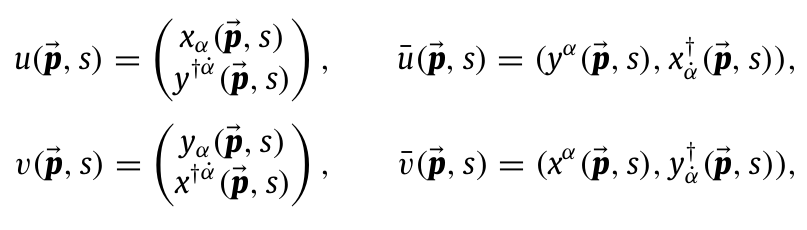
\includegraphics[scale=0.45]{uvxy}

\section{Mandelstam variables}

We can generalize the defintion of $s$ in eq.\eqref{eq:smv} to the full
Mandelstam variables \url{http://bolvan.ph.utexas.edu/~vadim/Classes/2011f/STU.pdf}, (See also \cite{Peskin})
\begin{align}
\label{eq:mvstu}
  s=&\left( p_1+p_2 \right)^2=\left( p_1'+p_2' \right)^2 \nonumber\\
  t=&\left( p_1-p_1' \right)^2=\left( p_2-p_2' \right)^2 \nonumber\\
  u=&\left( p_1-p_2' \right)^2=\left( p_1'-p_2 \right)^2 \,.
\end{align}
The explicit form for $s$ is
\begin{align}
  s=&\left( p_1+p_2 \right)^2 \nonumber\\
 =& p_1^2+p_2^2+2 p_1\cdot p_2 \nonumber\\
=& m_1^2+m_2^2+2 p_1\cdot p_2\,,
\end{align}
from which the product $p_1\cdot p_2$ can be obtained.  By following similar steps for $t$ and $u$, we have
\begin{align}
\label{eq:stucs}
  2 p_1\cdot p_2=&s- m_1^2-m_2^2 \nonumber\\
  2 p_1'\cdot p_2'=&s- {m_1'}^2-{m_2'}^2 \nonumber\\
  2 p_1\cdot p_1'=&m_1^2+{m_1'}^2 -t \nonumber\\
  2 p_2\cdot p_2'=&m_2^2+{m_2'}^2 -t \nonumber\\
  2 p_1\cdot p_2'=&m_1^2+{m_2'}^2 -u \nonumber\\
  2 p_2\cdot p_1'=&m_2^2+{m_1'}^2 -u \,.
\end{align}
Moreover,
\begin{align}
  s+t+u=m_1^2+m_2^2+{m_1'}^2+{m_2'}^2\,.
\end{align}

In the non-relativistic limit
\begin{align}
  s&=m_1^2+m_2^2   +2 p_1\cdot p_2 \approx (m_1+m_2)^2  + m_1m_2 (\mathbf{v}_1-\mathbf{v}_2)>0\,, \nonumber\\
  t&=m_1^2+{m_1'}^2-2 p_1\cdot p_1'\approx (m_1-m_1')^2 - m_1m_1' (\mathbf{v}_1-\mathbf{v}_1')>0\,,\nonumber\\
  u&=m_1^2+{m_2'}^2-2 p_1\cdot p_2'\approx (m_1-m_2')^2 - m_1m_2'  (\mathbf{v}_1-\mathbf{v}_2')>0\,.
\end{align}


\section{Yukawa interaction}
\label{sec:feynman-diagrams}
As a concrete example, we take a theory with a fermion field and scalar field, which interact via the Standard Model Yukawa interaction \cite{Lahiri:2005sm}. 
\begin{align}
\label{eq:lppp}
  \mathcal{L}_{\text{int}}=&-\frac{h}{\sqrt{2}}\phi\overline{\Psi}\Psi \nonumber\\
&=-y \phi \left[\left( \psi_R \right)^{\dagger}\psi_L+\left(\psi_L \right)^{\dagger}\psi_R  \right].
\end{align}
Let the quantum of the field $\phi$ be denoted by $H$, since the particle is a Higgs. The quanta of the fermionic field $f$ will be called electrons. The mass of $H$ is $M$, and the mass of the electron by $m$. Suppose $M\gt 2m$,  so that kinematically it is possible to have the $H$ particle decay into an electron-positron pair. The process is denoted by
\begin{align}
  H(k)\to e^-(p)+e^+(p')\,,
\end{align}
where $k$, $p$, $p'$ are the 4--momenta of the particles.

For the interaction Hamiltonian we have
\begin{align}
\label{eq:hppp}
  \mathcal{H}_I=\frac{h}{\sqrt{2}}:(\psi_R)^{\dagger}{\psi_L}\phi:
\end{align}
where the required ordered product will be explained in next section.
The term linear in the interaction Hamiltonian in the $S$--matrix.  It is
\begin{align}
  S^{(1)}=&-i \frac{h}{\sqrt{2}} \int d^4x:(\psi_R)^{\dagger}{\psi_L}\phi:\,.
\end{align}

\begin{align}
  S^{(1)}=-i \frac{h}{\sqrt{2}} \int d^4x:[(\psi_R)^{\dagger}_++(\psi_R)^{\dagger}_-]({\psi_L}_++{\psi_L}_-)(\phi_++\phi_-):\,.
\end{align}
where $+$ or $-$ denote the annihilation or creation operators respectively

\begin{align}
 \phi_{+} | n_{\phi} \rangle  \propto& |n-1_{\phi}\rangle & \langle n_{\phi}|\phi_{+} \propto& \langle n+1_{\phi}|
\end{align}

and

\begin{align}
 \phi_{-} |n_{\phi}\rangle  \propto& |n+1_{\phi}\rangle&  \langle n_{\phi}| \phi_{-} \propto& \langle n-1_{\phi}|
\end{align}

with similar expressions for fermion or vector fields.


Expanding the ordered product in the interaction Hamiltonian-densyty in eq.~\eqref{eq:hppp} in terms of the  $+$ and $-$ components of the several scalar and fermions fields, we have
\begin{align}
\label{eq:fullhppp}
 \mathcal{H}_{int}=&h:\left( (\psi_R)^{\dagger}_{+}+(\psi_R)^{\dagger}_{-}\right) \left( {\psi_L}_{+}+{\psi_L}_{-}\right) \left( \phi_{+}+\phi_{-}\right):\nonumber\\
=&h:
(\psi_R)^{\dagger}_{+}{\psi_L}_{+}\phi_{+}+ 
(\psi_R)^{\dagger}_{+}{\psi_L}_{+}\phi_{-}+ 
(\psi_R)^{\dagger}_{+}{\psi_L}_{-}\phi_{+}+ 
(\psi_R)^{\dagger}_{+}{\psi_L}_{-}\phi_{-}+ 
(\psi_R)^{\dagger}_{-}{\psi_L}_{+}\phi_{+}\nonumber\\ 
&+(\psi_R)^{\dagger}_{-}{\psi_L}_{+}\phi_{-}+ 
(\psi_R)^{\dagger}_{-}{\psi_L}_{-}\phi_{+}+ 
(\psi_R)^{\dagger}_{-}{\psi_L}_{-}\phi_{-} 
:\,.
\end{align}
The ordered product refers to the different from zero terms when the interaction Hamiltonian density is operated between the initial and final states, which for the decay processes under study correspond to
\begin{align}
  |i\rangle=&|0_{(\psi_R)^{\dagger}},0_{{\psi_L}},1_{\phi}\rangle & \text{and,} && \langle f|=&\langle 1_{(\psi_R)^{\dagger}},1_{{\psi_L}},0_\phi|
\end{align}
Evaluating the expectation values for each term in eq.~\eqref{eq:fullhppp} for these initial and final states, we have
\begin{align*}
 \langle1_{(\psi_R)^{\dagger}},1_{{\psi_L}},0_{\phi}|(\psi_R)^{\dagger}_{+}{\psi_L}_{+}\phi_{+}|0_{(\psi_R)^{\dagger}},0_{{\psi_L}},1_{\phi}\rangle  &\propto  \langle2_{(\psi_R)^{\dagger}},2_{{\psi_L}},0_{\phi}|0_{(\psi_R)^{\dagger}},0_{{\psi_L}},0_{\phi}\rangle =0\\ 
 \langle1_{(\psi_R)^{\dagger}},1_{{\psi_L}},0_{\phi}|(\psi_R)^{\dagger}_{+}{\psi_L}_{+}\phi_{-}|0_{(\psi_R)^{\dagger}},0_{{\psi_L}},1_{\phi}\rangle  &\propto  \langle2_{(\psi_R)^{\dagger}},2_{{\psi_L}},0_{\phi}|0_{(\psi_R)^{\dagger}},0_{{\psi_L}},2_{\phi}\rangle =0\\ 
 \langle1_{(\psi_R)^{\dagger}},1_{{\psi_L}},0_{\phi}|(\psi_R)^{\dagger}_{+}{\psi_L}_{-}\phi_{+}|0_{(\psi_R)^{\dagger}},0_{{\psi_L}},1_{\phi}\rangle  &\propto  \langle2_{(\psi_R)^{\dagger}},0_{{\psi_L}},0_{\phi}|0_{(\psi_R)^{\dagger}},0_{{\psi_L}},0_{\phi}\rangle =0\\ 
 \langle1_{(\psi_R)^{\dagger}},1_{{\psi_L}},0_{\phi}|(\psi_R)^{\dagger}_{+}{\psi_L}_{-}\phi_{-}|0_{(\psi_R)^{\dagger}},0_{{\psi_L}},1_{\phi}\rangle  &\propto  \langle2_{(\psi_R)^{\dagger}},0_{{\psi_L}},0_{\phi}|0_{(\psi_R)^{\dagger}},0_{{\psi_L}},2_{\phi}\rangle =0\\ 
 \langle1_{(\psi_R)^{\dagger}},1_{{\psi_L}},0_{\phi}|(\psi_R)^{\dagger}_{-}{\psi_L}_{+}\phi_{+}|0_{(\psi_R)^{\dagger}},0_{{\psi_L}},1_{\phi}\rangle  &\propto  \langle0_{(\psi_R)^{\dagger}},2_{{\psi_L}},0_{\phi}|0_{(\psi_R)^{\dagger}},0_{{\psi_L}},0_{\phi}\rangle =0\\ 
 \langle1_{(\psi_R)^{\dagger}},1_{{\psi_L}},0_{\phi}|(\psi_R)^{\dagger}_{-}{\psi_L}_{+}\phi_{-}|0_{(\psi_R)^{\dagger}},0_{{\psi_L}},1_{\phi}\rangle  &\propto  \langle0_{(\psi_R)^{\dagger}},2_{{\psi_L}},0_{\phi}|0_{(\psi_R)^{\dagger}},0_{{\psi_L}},2_{\phi}\rangle =0\\ 
 \langle1_{(\psi_R)^{\dagger}},1_{{\psi_L}},0_{\phi}|(\psi_R)^{\dagger}_{-}{\psi_L}_{-}\phi_{+}|0_{(\psi_R)^{\dagger}},0_{{\psi_L}},1_{\phi}\rangle  &\propto  \langle0_{(\psi_R)^{\dagger}},0_{{\psi_L}},0_{\phi}|0_{(\psi_R)^{\dagger}},0_{{\psi_L}},0_{\phi}\rangle \neq 0\\
 \langle1_{(\psi_R)^{\dagger}},1_{{\psi_L}},0_{\phi}|(\psi_R)^{\dagger}_{-}{\psi_L}_{-}\phi_{-}|0_{(\psi_R)^{\dagger}},0_{{\psi_L}},1_{\phi}\rangle  &\propto  \langle0_{(\psi_R)^{\dagger}},0_{{\psi_L}},0_{\phi}|0_{(\psi_R)^{\dagger}},0_{{\psi_L}},2_{\phi}\rangle =0
\end{align*}
In this way, we have

\begin{align}
:(\psi_R)^{\dagger}{\psi_L}\phi: =&(\psi_R)^{\dagger}_{-}{\psi_L}_{-}\phi_{+}\,.
\end{align}
In general, we have the following result: The ordered product of a set of operators is such that all the creation operators are on the left and destruction operators are in the right while keeping the original order consistent with the initial and final states.
\begin{align}
\langle 1,1,\cdots,0,0|  :\phi_1 \phi_2 \cdots \phi_{n-1}\phi_n:|0,0,\cdots,1,1\rangle
\propto \langle 1,1,\cdots,0,0| a_1^{\dagger} a_2^{\dagger}\cdots a_{n-1}a_n|0,0,\cdots,1,1\rangle
\end{align}


The only term that contributes to the matrix element of these process is therefore
\begin{align}
  \label{eq:97f}
  -i \frac{h}{\sqrt{2}} \int d^4x(\psi_R)^{\dagger}_-{\psi_L}_-\phi_+\,.
\end{align}

\begin{figure} %noinstiki
  \centering %noinstiki
  \includegraphics[scale=0.6]{Btoee} %noinstiki
  \caption{Feynman diagrams for $B\to e^+ e^-$} %noinstiki
  \label{fig:btoee} %noinstiki
\end{figure} %noinstiki
In the language of second quantization it is said that at the interaction point in Fig.~\ref{fig:btoee}, the scalar is destroyed by $\phi_+$ and one electron (${\psi_L}_-$) and a positron ($(\psi_R)^{\dagger}_{-}$) are created.

Let us define the one--particle states as in eq.~\eqref{eq:38f}

\begin{align}
  | H(\mathbf{p})\rangle\equiv\sqrt{\frac{1}{V}}a^\dagger_{\mathbf{p}}|0\rangle 
\end{align}
For the two Weyl spinors forming a Dirac spinor we have the solutions
\begin{align}
 e_L\to \xi_{\alpha}=&\sum_s\int \frac{\operatorname{d}^3p}{(2\pi)^3\sqrt{2E_{\mathbf{p}}}} \left[ x_{\alpha}\left(s,\mathbf{p}\right) a_s e^{-i p\cdot x}+y_{\alpha}\left(s,\mathbf{p}\right) b_s^{\dagger} e^{i p\cdot x}  \right]\nonumber\\
 \left( e_L \right)^{\dagger}\to \xi_{\dot{\alpha}}^{\dagger}=&\sum_s\int \frac{\operatorname{d}^3p}{(2\pi)^3\sqrt{2E_{\mathbf{p}}}} \left[ y_{\dot{\alpha}}^{\dagger}\left(s,\mathbf{p}\right) b_s e^{-i p\cdot x}+x_{\dot{\alpha}}^{\dagger}\left(s,\mathbf{p}\right) a_s^{\dagger} e^{i p\cdot x}  \right]\nonumber\\
 \left( e_R \right)^{\dagger}\to \eta^{\alpha}=&\sum_s\int \frac{\operatorname{d}^3p}{(2\pi)^3\sqrt{2E_{\mathbf{p}}}} \left[ x^{\alpha}\left(s,\mathbf{p}\right) b_s e^{-i p\cdot x}+y^{\alpha}\left(s,\mathbf{p}\right) a_s^{\dagger} e^{i p\cdot x}  \right] \nonumber\\
  e_R\to \eta^{\dagger\dot{\alpha}}=&\sum_s\int \frac{\operatorname{d}^3p}{(2\pi)^3\sqrt{2E_{\mathbf{p}}}} \left[ y^{\dagger\dot{\alpha}}\left(s,\mathbf{p}\right) a_s e^{-i p\cdot x}+x^{\dagger\dot{\alpha}}\left(s,\mathbf{p}\right) b_s^{\dagger} e^{i p\cdot x}  \right].
\end{align}


From here we can define the one--particle states as
\begin{align}
  \label{eq:77f}
   | e_L(\mathbf{p},s)\rangle\equiv&\sqrt{\frac{1}{V}}a^\dagger_s(\mathbf{p})|0\rangle, &    | e_R(\mathbf{p},s)\rangle\equiv&\sqrt{\frac{1}{V}}a^\dagger_s(\mathbf{p})|0\rangle\nonumber\\
   | \left( e_L \right)^{\dagger}(\mathbf{p},s)\rangle\equiv&\sqrt{\frac{1}{V}}{b}^\dagger_s(\mathbf{p})|0\rangle,&
   | \left( e_R \right)^{\dagger}(\mathbf{p},s)\rangle\equiv&\sqrt{\frac{1}{V}}{b}^\dagger_s(\mathbf{p})|0\rangle\,, 
\end{align}
Using the commutation relations, our states are then normalized as
\begin{align}
\langle H(\mathbf{p})| H(\mathbf{p}')\rangle=&\frac{(2\pi)^3}{V}\delta^3(\mathbf{p}-\mathbf{p}')\nonumber\\
\langle e_{L,R}(\mathbf{p},s)| e_{L,R}(\mathbf{p}',s')\rangle=&\frac{(2\pi)^3}{V}\delta_{s s'}\delta^3(\mathbf{p}-\mathbf{p}')\nonumber\\
\langle \left( e_{L,R} \right)^{\dagger}(\mathbf{p},s)| \left( e_{L,R} \right)^{\dagger}(\mathbf{p}',s')\rangle=&\frac{(2\pi)^3}{V}\delta_{s s'}\delta^3(\mathbf{p}-\mathbf{p}')
\end{align}
As established in Sec.~\ref{sec:fock-space-real}, it is convenient to work in the discrete limit where \eqref{eq:26f}
\begin{align}
   \delta^3(\mathbf{0})=\frac{V}{(2\pi)^3}\,.
\end{align}

Now we can write down the action of various field operators on different one particles states. 
Using the Fourier decomposition  of the scalar field in eq.~\eqref{eq:37f}, and taking into account that 
$a_{\mathbf{p}}|0\rangle=0$, we have
\begin{align}
\label{eq:98f}
   \phi_+(x)|H(\mathbf{k})\rangle=&\int d^3p \frac{1}{(2\pi)^3\sqrt{2\omega_{p} }}
\widehat{a}_{p} e^{-i p\cdot x }
|H(\mathbf{k})\rangle\nonumber\\
=&\int d^3p \frac{1}{(2\pi)^3\sqrt{2\omega_{p}}}
\widehat{a}_\mathbf{p} e^{-i p\cdot x }
\frac{1}{\sqrt{V}}\, \widehat{a}^\dagger_{\mathbf{k}}|0\rangle\nonumber\\
  =&\int d^3p \frac{1}{(2\pi)^3\sqrt{2\omega_{p}V}} e^{-i p\cdot x }
\, [\widehat{a}_{\mathbf{p}},\widehat{a}^\dagger_{\mathbf{k}}]|0\rangle\,.
\end{align}
%check normalization!
By using the commutation relations in eq.~\eqref{eq:32f} we have

\begin{align}
\phi_+(x)|H(\mathbf{k})\rangle  
=&\int d^3p \frac{\delta^{(3)}(\mathbf{p}-\mathbf{k})}{\sqrt{2\omega_{p}V}}
 e^{-i p\cdot x }|0\rangle
\end{align}
\begin{align}
\phi_+(x)|H(\mathbf{k})\rangle  
=&\frac{1}{\sqrt{2\omega_{k}V}}e^{-i k\cdot x }|0\rangle
\end{align}
Similarly, we have  \emph{initial one-particles states} on left and \emph{initial one-particles states} on right
\begin{align}
  \label{eq:99f}
  \phi_+(x)|H(\mathbf{k})\rangle=&\frac{1}{\sqrt{2 \omega_k V}}e^{-i k\cdot x}|0\rangle,&
 \langle H(\mathbf{k})|\phi_-(x)=&\langle0|\frac{1}{\sqrt{2 \omega_k V}}e^{i k\cdot x}\nonumber\\
  \xi_+(x)|e_{L}(\mathbf{p},s)\rangle=&\frac{1}{\sqrt{2 E_p V}}x(s,\mathbf{p})e^{-i p\cdot x}|0\rangle,&
  \langle e_{L}(\mathbf{p},s)|\xi_-^{\dagger}(x)=&\langle 0|\frac{1}{\sqrt{2 E_p V}}x^{\dagger}(s,\mathbf{p})e^{i p\cdot x}\nonumber\\
  \eta_+(x)|\left( e_R \right)^{\dagger}(\mathbf{p},s)\rangle=&\frac{1}{\sqrt{2 E_{p} V}}x(s,\mathbf{p})e^{-i p\cdot x}|0\rangle,&
  \langle \left( e_R \right)^{\dagger}(\mathbf{p},s)|\eta^{\dagger}_-(x)=&\langle 0|\frac{1}{\sqrt{2 E_{p} V}}x^{\dagger}(s,\mathbf{p})e^{i p\cdot x} \nonumber\\
  \xi_+^{\dagger}(x)|\left( e_{L} \right)^{\dagger}(\mathbf{p},s)\rangle=&\frac{1}{\sqrt{2 E_p V}}y^{\dagger}(s,\mathbf{p})e^{-i p\cdot x}|0\rangle,&
  \langle\left( e_{L} \right)^{\dagger}(\mathbf{p},s)|\xi_-(x)=&\langle 0| \frac{1}{\sqrt{2 E_p V}}y(s,\mathbf{p})e^{i p\cdot x}\nonumber\\
  \eta_+^{\dagger}(x)|e_R (\mathbf{p},s)\rangle=&\frac{1}{\sqrt{2 E_{p} V}}y^{\dagger}(s,\mathbf{p})e^{-i p\cdot x}|0\rangle,&
  \langle e_R(\mathbf{p},s)|\eta_-(x)=&\langle 0|\frac{1}{\sqrt{2 E_{p'} V}}y(s,\mathbf{p})e^{i p\cdot x}
 \,.
\end{align}
where $\omega_k$ and $E_p$ represent the energies of the scalar and the electron for the 3-momenta in the subscripts.

In the lowest order the only term which contributes to the matrix element is the term shown in Eq.~\eqref{eq:97f}.
The matrix element at first order in eq.~\eqref{eq:S1}, between the initial and the final state is then
\begin{align}
  S_{fi}^{(1)}=-i \frac{h}{\sqrt{2}} \sum_{s,s'} \int \operatorname{d}^4x &\left[ \left\langle 0, e_L(\boldsymbol{p}),\left( e_R \right)^{\dagger}(
\boldsymbol{p}') \left|\xi_-^{\dagger}(x)\eta_-^{\dagger}(x) \phi_{+}(x)  \right|H(\mathbf{k}),0,0 \right\rangle
   \right. +\nonumber\\
&\left.\left\langle 0,\left( e_L \right)^{\dagger}(\boldsymbol{p}), e_R (\boldsymbol{p}') \right|\xi_-(x)\eta_-(x) \phi_{+}(x)  \left|H(\mathbf{k}),0,0 \right\rangle \right] 
\end{align}
Using Eqs.~\eqref{eq:99f}  we obtain
\begin{align}
  S_{fi}^{(1)}=&(-i )\frac{h}{\sqrt{2}}  \sum_{s,s'}\left[ x^{\dagger}_{\dot{\alpha}}(s,\boldsymbol{p}){x^{\dagger}}^{\dot{\alpha}}(s',\boldsymbol{p}')+y^{\alpha}(s,\boldsymbol{p})y_{\alpha}(s',\boldsymbol{p}') \right] \nonumber\\
&\times\int d^4x\,e^{i(p+p'-k)\cdot x}\frac{1}{\sqrt{2\omega_k V}}\frac{1}{\sqrt{2E_p V}}\frac{1}{\sqrt{2E_{p'} V}}\,.
\end{align}
Since
\begin{align}
  \int d^4x\,e^{i(p+p'-k)\cdot x}=(2\pi)^4\delta^4(k-p-p')\,,
\end{align}
we obtain
\begin{align}
  S_{fi}^{(1)}=&\left[\frac{1}{\sqrt{2\omega_k V}}\frac{1}{\sqrt{2E_p V}}\frac{1}{\sqrt{2E_{p'} V}}\right]
(2\pi)^4\delta^4(k-p-p') \nonumber\\
&\times(-i )\frac{h}{\sqrt{2}}\sum_{s,s'}\left[ x^{\dagger}_{\dot{\alpha}}(s,\boldsymbol{p}){x^{\dagger}}^{\dot{\alpha}}(s',\boldsymbol{p}')+y^{\alpha}(s,\boldsymbol{p})y_{\alpha}(s',\boldsymbol{p}') \right].
\end{align}
Comparing with Eq.~\eqref{eq:RMfi} we have therefore that the relativistic \emph{amplitude} is
\begin{align}
\label{eq:calm}
  i\mathcal{M}_{fi}=-i \frac{h}{\sqrt{2}}\sum_{s,s'}\left[ x^{\dagger}_{\dot{\alpha}}(s,\boldsymbol{p}){x^{\dagger}}^{\dot{\alpha}}(s',\boldsymbol{p}')+y^{\beta}(s,\boldsymbol{p})y_{\beta}(s',\boldsymbol{p}') \right].
\end{align}
Check the specific calculation in~\ref{Dreiner:2008tw}

The equation for a two body decays, assuming that the amplitude \eqref{eq:calm} does not depends in the final momentum,  is given in eq.~\eqref{eq:152} is 
\begin{align}
\label{eq:154pdn}
\frac{d\Gamma}{d\Omega}=
&\frac{1}{64 \pi^2M^3}\left|\mathcal{M}_{fi}\right|^2\lambda^{1/2}(M^2,m_2^2,m_1^2)
\end{align}
where, from \eqref{eq:46}
\begin{align}
\label{eq:46n}
  \lambda(a,b,c)=\left[ a-(b-c) \right]^2-4ac\,.
\end{align}

For our specific problem, the final state masses of electron and positron is the same, however, we will obtain the results for the most general case of different masses. In this way, let $m$ ($m'=m$) the mass of $e_L$ ($e_R$).

The missing part is to calculate the square of the amplitude
\begin{align}
  \left| \mathcal{M} \right|^2=&\mathcal{M}^{\dagger}M= \nonumber\\
=&\frac{h^{2}}{2}\sum_{s,s'}
 \left[ x^{\dagger}_{\dot{\alpha}}(s,\boldsymbol{p}){x^{\dagger}}^{\dot{\alpha}}(s',\boldsymbol{p}')+y^{\beta}(s,\boldsymbol{p})y_{\beta}(s',\boldsymbol{p}') \right]^{\dagger}
\left[ x^{\dagger}_{\dot{\alpha}}(s,\boldsymbol{p}){x^{\dagger}}^{\dot{\alpha}}(s',\boldsymbol{p}')+y^{\beta}(s,\boldsymbol{p})y_{\beta}(s',\boldsymbol{p}') \right] \nonumber\\
  =&\frac{h^2}{2}\sum_{s,s'} \left[x^{\alpha}(s',\boldsymbol{p}') x_{\alpha}(s,\boldsymbol{p})+y^{\dagger}_{\dot{\beta}}(s',\boldsymbol{p}')y^{\dagger\dot{\beta}}(s,\boldsymbol{p}) \right]
\left[ x^{\dagger}_{\dot{\alpha}}(s,\boldsymbol{p}){x^{\dagger}}^{\dot{\alpha}}(s',\boldsymbol{p}')+y^{\beta}(s,\boldsymbol{p})y_{\beta}(s',\boldsymbol{p}') \right],
\end{align}

 which includes (using anticommuting spinors)
\begin{align}
\sum_{s,s'}x^{\alpha}(s',\boldsymbol{p}') x_{\alpha}(s,\boldsymbol{p})
x^{\dagger}_{\dot{\alpha}}(s,\boldsymbol{p}){x^{\dagger}}^{\dot{\alpha}}(s',\boldsymbol{p}') 
&= \sum_{s'}x^{\alpha}(s',\boldsymbol{p}')  \left[ 
\sum_{s} x_{\alpha}(s,\boldsymbol{p})x^{\dagger}_{\dot{\alpha}}(s,\boldsymbol{p})\right]
{x^{\dagger}}^{\dot{\alpha}}(s',\boldsymbol{p}')  \nonumber\\
&= \sum_{s'}x^{\alpha}(s',\boldsymbol{p}') \left( p\cdot \sigma_{\alpha{\dot{\alpha}}}  \right)
{x^{\dagger}}^{\dot{\alpha}}(s',\boldsymbol{p}')  \nonumber\\
&=\left( p\cdot \sigma_{\alpha{\dot{\alpha}}}  \right) \sum_{s'} {x^{\dagger}}^{\dot{\alpha}}(s',\boldsymbol{p}') x^{\alpha}(s',\boldsymbol{p}')  \nonumber\\
&=\left( p\cdot \sigma_{\alpha{\dot{\alpha}}}  \right) \left( p'\cdot \overline{\sigma}_{\dot{\alpha}\alpha} \right) \nonumber\\
&=\operatorname{Tr}\left[ \left( p\cdot \sigma \right)\left( p'\cdot \overline{\sigma} \right)  \right] \nonumber\\
&=p_{\mu}p'_{\nu}\operatorname{Tr}\left[ \sigma^{\mu} \overline{\sigma}^{\nu}  \right] \nonumber\\ 
&=2 g^{\mu\nu}p_{\mu}p'_{\nu} \nonumber\\
&=2 p\cdot p'\,.
\end{align}

\begin{align}
\sum_{s,s'}y^{\dagger}_{\dot{\beta}}(s',\boldsymbol{p}')y^{\dagger\dot{\beta}}(s,\boldsymbol{p})y^{\beta}(s,\boldsymbol{p})y_{\beta}(s',\boldsymbol{p}')
=&  \left( p\cdot \overline{\sigma}^{\dot{\beta}\beta} \right)\sum_{s,s'}y^{\dagger}_{\dot{\beta}}(s',\boldsymbol{p}')y_{\beta}(s',\boldsymbol{p}') \nonumber\\
=&  \left( p\cdot \overline{\sigma}^{\dot{\beta}\beta} \right) \sum_{s,s'}y_{\beta}(s',\boldsymbol{p}')y^{\dagger}_{\dot{\beta}}(s',\boldsymbol{p}') \nonumber\\
=&  \left( p\cdot \overline{\sigma}^{\dot{\beta}\beta} \right) \left( p'\cdot \sigma_{\beta \dot{\beta}} \right) \nonumber\\
=& 2 p \cdot p'\,.
\end{align}

\begin{align}
  \sum_{s,s'}x^{\alpha}(s',\boldsymbol{p}') x_{\alpha}(s,\boldsymbol{p})y^{\beta}(s,\boldsymbol{p})y_{\beta}(s',\boldsymbol{p}') =& 
  \sum_{s'}x^{\alpha}(s',\boldsymbol{p}') \left[ \sum_{s} x_{\alpha}(s,\boldsymbol{p})y^{\beta}(s,\boldsymbol{p}) \right]y_{\beta}(s',\boldsymbol{p}') \nonumber\\
 =& \left(m{\delta_{\alpha}}^{\beta}  \right) \sum_{s'}  y_{\beta}(s',\boldsymbol{p}')x^{\alpha}(s',\boldsymbol{p}') \nonumber\\
 =& \left(m{\delta_{\alpha}}^{\beta}  \right)  \left(- m'{{\delta_{\beta}}^{\alpha}}  \right) \nonumber\\
 =& \operatorname{Tr} \left[ -m m'  \boldsymbol{1} \boldsymbol{1} \right] \nonumber\\
 =& mm'\operatorname{Tr} \left[  \boldsymbol{1} \right] \nonumber\\
 =& -2 mm'\,.
\end{align}

\begin{align}
  \sum_{s,s'}y^{\dagger}_{\dot{\beta}}(s',\boldsymbol{p}')y^{\dagger\dot{\beta}}(s,\boldsymbol{p})x^{\dagger}_{\dot{\alpha}}(s,\boldsymbol{p}){x^{\dagger}}^{\dot{\alpha}}(s',\boldsymbol{p}')  
=&   \left( m {\delta^{\dot{\beta}}}_{\dot{\alpha}} \right) \left( -m' {\delta}^{\dot{\alpha}}_{\dot{\beta}} \right) \nonumber\\
=& -2m m'\,.
\end{align}
Therefore
\begin{align}
   \left| \mathcal{M} \right|^2=4 \frac{h^{2}}{2} \left( p\cdot p' - mm' \right)
\end{align}

From eq.~\eqref{eq:153}
\begin{align}
  M=&E+{E'}\nonumber\\
|\mathbf{p}|&=|\mathbf{p}'|
\end{align}
Therefore
\begin{align}
  E{E'}=\frac{M^2-E^2-{E'}^2}{2}
\end{align}
\begin{align*}
  p\cdot p'-m {m'}&=EE'-\mathbf{p}_{1}\cdot\mathbf{p}_{2}-m {m'}\\
&=EE'+\mathbf{p}^2-m {m'}\\
&=\frac{M^2-E^2-{E'}^2}{2}+\mathbf{p}^2-m {m'}\nonumber\\
&=\frac12\left(M^2-m^2-\mathbf{p}^2-{m'}^2-\mathbf{p}^2\right)+\mathbf{p}^2-m {m'}\\
&=\frac12\left(M^2-m^2-{m'}^2-2m{m'}\right)\\
&=\frac12\left[M^2-(m-{m'})^2\right]
\end{align*}
%\left(\right)
Therefore, the scattering  amplitude is
\begin{equation}
\sum_{s_1,s_2}|\mathcal{M}|^{2}=h^2\left[M^2-(m+{m'})^2\right]
\end{equation}
Since this does not depends explicitly on the final state tri-momentum, is was consistent to already make the tri-momentum integrals. Moreower, Replacing back in eq.~\eqref{eq:154pdn}
\begin{align}
\frac{d\Gamma}{d\Omega}=
&\frac{h^2}{64 \pi^2M^3}\lambda^{1/2}(M^2,{m'}^2,m^2)\left[M^2-(m+{m'})^2\right]
\end{align}
After the integration $\int d\Omega_{\text{CM}}=4\pi$\footnote{$\int_0^{2\pi}d\phi\int_0^\pi\sin\theta d\theta=4\pi $} we have
\begin{align}
\Gamma=&\frac{h^2}{16 \pi M^3}\lambda^{1/2}(M^2,{m'}^2,m^2)\left[M^2-(m+{m'})^2\right]
\end{align}
For $m={m'}=m_f$, and using eq.~\eqref{eq:46n}


\begin{align}
  \lambda^{1/2}(M^2,m^2_f,m_f^2)=&
  \left[ \left( M^2-m^2_f+m^2_f  \right)^2-4 M^2m_f^2  \right]^{1/2}\nonumber\\
  =&\left( M^4-4 M^2m_f^2  \right)^{1/2}\nonumber\\
  =&\left[M^4 \left( 1-4 \frac{m_f^2}{M^2} \right) \right]^{1/2}\nonumber\\
  =&M^2 \left( 1-4 \frac{m_f^2}{M^2} \right)^{1/2}\,,
\end{align}
and therefore
\begin{align}
\Gamma(H\to f\overline{f})=&\frac{h^2}{16 \pi M^3}M^2 \left( 1-4 \frac{m_f^2}{M^2} \right)^{1/2}
 \left[M^2-4m_f^2\right] \nonumber\\
=&\frac{h^2}{16 \pi M^3}M^4 \left( 1-4 \frac{m_f^2}{M^2} \right)^{1/2}
 \left[1-4 \frac{m_f^2}{M^2}\right] \nonumber\\
=&\frac{h^2}{16 \pi}M\left(1-\frac{4m_f^2}{M^2}\right)^{3/2}
\end{align}
In the case of the standard model Higgs with mass $M_H=M$ decaying to fermion pair, and using $m_f=hv/\sqrt{2}$,  $v=\left( \sqrt{2}G_F \right)^{-1/2}$

\begin{align}
\Gamma(H\to f\overline{f})=&\frac{h^2v^2}{16 v^2 \pi}M_H\left(1-\frac{4m_f^2}{M_H^2}\right)^{3/2} \nonumber\\
=&\frac{h^2v^2}{2}\frac{1}{8 v^2 \pi}M_H\left(1-\frac{4m_f^2}{M_H^2}\right)^{3/2} \nonumber\\
=&m_f^2\frac{\sqrt{2}G_F}{8\pi}M_H\left(1-\frac{4m_f^2}{M_H^2}\right)^{3/2} \nonumber\\
&=\frac{M_{H}m_{f}^{2}G_{F}}{4\pi\sqrt{2}}
\left(1-4\frac{m^2_{f}}{M^2_{H}}\right)^{3/2}, 
\end{align}

In the limit $m_{f}\ll M_{H}$ this expression reduces to 
\begin{equation}
\Gamma(H\to
f\overline{f})=\frac{M_{H}m_{f}^{2}G_{F}}{4\pi\sqrt{2}}. 
\end{equation}
For the tau\footnote{to the top quarks is kinematically forbidden, to the bottom quark a further factor $N_c=3$ must be considered}, taking into account that $1.166 \times 10^{-5}\ \text{GeV}^{-2}$, $M_H=125\ \text{GeV}$, and $m_\tau=1.777\ \text{GeV}$,
\begin{align}
  \Gamma(H\to \tau^+\tau^-)=0.26\ \text{MeV}\to \tau= \frac{\hbar}{\Gamma}=2.53\times 10^{-21}\ \text{seconds}\,.
\end{align}




% \subsection{Yukawa interaction for Weyl fermions}
% Left-handed fermion:
% \begin{align}
% %e_L -> e_L^- + (e_R^+)^{\dagger}
% e_L\to  \xi_{\alpha}=&\int \frac{d^3 p}{(2\pi)^3\sqrt{2E_{\mathbf{p}}}} \left[ x_{\alpha}(\mathbf{p},s)a(\mathbf{p},s)\operatorname{e}^{-i p\cdot x}+y_{\alpha}(\mathbf{p},s)a^{\dagger}(\mathbf{p},s)\operatorname{e}^{i p\cdot x} \right] \nonumber\\
% %(e_L)^{\dagger} -> e_R^+ + (e_L^-)^{\dagger}
% \left( e_L \right)^{\dagger}\to  \xi_{\dot{\alpha}}^{\dagger}=&\int \frac{d^3 p}{(2\pi)^3\sqrt{2E_{\mathbf{p}}}} \left[y_{\dot{\alpha}}^{\dagger}(\mathbf{p},s)a(\mathbf{p},s)\operatorname{e}^{-i p\cdot x}+ x_{\dot{\alpha}}^{\dagger}(\mathbf{p},s)a^{\dagger}(\mathbf{p},s)\operatorname{e}^{i p\cdot x}\right] .
% \end{align}

% Right-handed fermion 
% \begin{align}
% %e_R -> e_R^- + (e_L^+)^{\dagger}
% e_R\to  \eta^{\dagger\dot{\alpha}}=&\int \frac{d^3 p}{(2\pi)^3\sqrt{2E_{\mathbf{p}}}} \left[y^{\prime\dot{\alpha}\dagger}(\mathbf{p},s)b(\mathbf{p},s)\operatorname{e}^{-i p\cdot x}+ x^{\prime\dot{\alpha}\dagger}(\mathbf{p},s)b^{\dagger}(\mathbf{p},s)\operatorname{e}^{i p\cdot x} \right] .
%  \nonumber\\
% %(e_R)^{\dagger} -> e_L^+ + (e_R^-)^{\dagger}
% \left( e_R \right)^{\dagger}\to  \eta^{\alpha}=&\int \frac{d^3 p}{(2\pi)^3\sqrt{2E_{\mathbf{p}}}} \left[ x^{\prime\alpha}(\mathbf{p},s)b(\mathbf{p},s)\operatorname{e}^{-i p\cdot x}+y^{\prime\,\alpha}(\mathbf{p},s)b^{\dagger}(\mathbf{p},s)\operatorname{e}^{i p\cdot x} \right]
% \end{align}
% \begin{align}
%  \xi_{+} | e^{-}_{L}\rangle =& x a a^{\dagger} |0\rangle \nonumber\\
%  \eta_{+} | \left( e^{-}_{R} \right)^{\dagger}\rangle =& x' b b^{\dagger} |0\rangle \nonumber\\
%  \xi_{+} |  \left( e^{-}_{L} \right)^{\dagger} \rangle =& y^{\dagger} a a^{\dagger} |0\rangle \nonumber\\
%  \eta_{+} | e^{-}_{R} \rangle =& y^{\prime \dagger} b b^{\dagger} |0\rangle
% \end{align}
% After some calcultations ...

% From the cojugate relations, e.g $\langle e_L^- |\xi_-=\langle 0|x^{\dagger}...$, etc
% \begin{align}
%   \mathcal{M}_1 =& x^{\dagger} x^{\prime \dagger} &\mathcal{M}_2=& y y'
% \end{align}
\section{Wick Theorem}
\label{sec:wick-theorem}

\subsection{Basics concepts}
Return back to  the interpretation of interaction in terms of one exchanged particle, as illustrated again in Fig.~\ref{fig:qedrepulsionx1x2}
\begin{figure}
  \centering
  \includegraphics{qedrepulsionx1x2}
  \caption{Electromagnetic repulsion. The diagrams (a) and (b) are summarized in the diagram (c)}
  \label{fig:qedrepulsionx1x2}
\end{figure}


From \cite{Lahiri:2005sm}. The normal ordering procedure involved putting all the annihilation operators to the right of all creation operators so that it annihilates the vacuum. But the time ordering raises complications because in it all operators at earlier times must be further to the right. So creation operators at later times would be to the right of annihilation operators at later times, contrary to what we need for normal ordering. The advantage of normal ordered products is that their expectation values vanish in the vacuum. 

If $H_I$ contains an even number of fermion factors, we can use the time--ordered product $\operatorname{T}\{\ldots\}$ of $n$ factors to write this expression in the equivalent form. For $S^{(2)}$ we have for example
\begin{align}
 \int_{-\infty}^\infty dt_1 \int_{-\infty}^{\infty}d t_2 \operatorname{T}\{H_I(t_1)H_I(t_2)\}=&
\int_{-\infty}^\infty dt_1\int_{-\infty}^{\infty}d t_2 \theta(t_2-t_1)H_I(t_2)H_I(t_1) \nonumber\\
&+\int_{-\infty}^\infty dt_1\int_{-\infty}^{\infty}d t_2 \theta(t_1-t_2)H_I(t_1)H_I(t_2)
 \end{align}
where, for $t_2$ and $t_1$ fixed respectively
 \begin{align}
   \theta(t_2-t_1)=&
   \begin{cases}
    0\, &    t_1> t_2\\
    1\, &    t_1< t_2\\
   \end{cases},&   \theta(t_1-t_2)=&
   \begin{cases}
    0\, &    t_2> t_1\\
    1\, &    t_2< t_1\\
   \end{cases}\,.
 \end{align}
In this way.
\begin{align}
 \int_{-\infty}^\infty dt_1 \int_{-\infty}^{\infty}d t_2 \operatorname{T}\{H_I(t_1)H_I(t_2)\}=&
\int_{-\infty}^\infty dt_2\int_{-\infty}^{t_2}d t_1 \theta(t_2-t_1)H_I(t_2)H_I(t_1)\nonumber\\
&+\cancel{\int_{-\infty}^\infty dt_2\int_{t_2}^{t_1}d t_1 \theta(t_2-t_1)H_I(t_2)H_I(t_1)} \nonumber\\
&+\int_{-\infty}^\infty dt_1\int_{-\infty}^{t_{1}}d t_2 \theta(t_1-t_2)H_I(t_1)H_I(t_2) \nonumber\\
&+\cancel{\int_{-\infty}^\infty dt_1\int_{t_1}^{t_2}d t_2 \theta(t_1-t_2)H_I(t_1)H_I(t_2)}\,.
\end{align}
The integral in $dt_1$ is for $t_1>t_2$, with $t_2$ fixed, so that $\theta(t_2-t_1)=0$ for $t_1>t_2$. Similarly,
The integral in $dt_2$ is for $t_2>t_1$, with $t_1$ fixed, so that $\theta(t_1-t_2)=0$ for $t_2>t_1$. Therefore,
\begin{align}
   \int_{-\infty}^\infty dt_1 \int_{-\infty}^{\infty}d t_2 \operatorname{T}\{H_I(t_1)H_I(t_2)\}=&
\int_{-\infty}^\infty dt_2\int_{-\infty}^{t_2}d t_1 H_I(t_2)H_I(t_1)
+\int_{-\infty}^\infty dt_1\int_{-\infty}^{t_{1}}d t_2 H_I(t_1)H_I(t_2)\nonumber\\
=&
\int_{-\infty}^\infty dt_1\int_{-\infty}^{t_1}d t_2 H_I(t_1)H_I(t_2)
+\int_{-\infty}^\infty dt_1\int_{-\infty}^{t_{1}}d t_2 H_I(t_1)H_I(t_2) \nonumber\\
=&
2\int_{-\infty}^\infty dt_1\int_{-\infty}^{t_1}d t_2 H_I(t_1)H_I(t_2)\,.
\end{align}
In terms of the ordering operator all the integrals are between $-\infty$ to $\infty$:
\begin{align}
   S=&1+\sum_{n=1}^\infty\frac{(-i)^n}{n!}\int_{-\infty}^{\infty}d t_1\,\int_{-\infty}^{\infty} d t_2\ldots\int_{-\infty}^{\infty}d t_n\,\operatorname{T}\{{H}_I(t_1){H}_I(t_2)\ldots{H}_I(t_n)\}\,, 
\end{align}
In terms of the Hamiltonian density, we have
\begin{align}
  S=1+\sum_{n=1}^\infty\frac{(-i)^n}{n!}\int\cdots\int d^4x_1 d^4x_2\ldots d^4x_n\,\operatorname{T}\{\mathcal{H}_I(x_1)\mathcal{H}_I(x_2)\ldots\mathcal{H}_I(x_n)\}\,, 
\end{align}
In the above perturbation formalism the states $|i\rangle$ and $|f\rangle$ are, as usual, eigenstates of the unperturbed free-field Hamiltonian $H_0$. As such can be introduced inside the integrals
\begin{align}
  S_{f i}=&\langle f|S|i\rangle\nonumber\\
  =&1+\sum_{n=1}^\infty\frac{(-i)^n}{n!}\int\cdots\int d^4x_1 d^4x_2\ldots d^4x_n\,\langle f|\operatorname{T}\{\mathcal{H}_I(x_1)\mathcal{H}_I(x_2)\ldots\mathcal{H}_I(x_n)\}|i\rangle\,.
\end{align}


For example, at first order
\begin{align}
  \label{eq:96f}
  S_{fi}^{(1)}=&\langle f|S^{(1)}|i\rangle\nonumber\\
  =&\langle f|-i\int d^4x_1\,\operatorname{T}\{\mathcal{H}_I(x_1)\}|i\rangle\nonumber\\
  =&-i\int d^4x_1\,\langle f|:\mathcal{H}_I(x_1):|i\rangle\,.
\end{align}
In order to evaluate this integrals we need to write the time ordered product in terms of the fields. This can done by induction. We start by considering the simple no trivial case with two scalar fields
%ver cuaderno de perrito


\subsection{Scalar propagator}

%copy and paste from scanned pages below
With
\begin{align}
  \bcontraction{\,}{\phi}{(x_1)}{\phi}
\,\phi(x_1)\phi(x_2)\equiv \left\langle 0 |   T\{\phi(x_1)\phi(x_2)\} | 0 \right\rangle
\end{align}




The Wick contraction can be written as:
\begin{align}
\label{eq:77f}
  \bcontraction{\,}{\phi}{(x_1)}{\phi}
\,\phi(x_1)\phi(x_2)=&\langle0|T\{\phi(x_1)\phi(x_2)\}|0\rangle\nonumber\\
=&i\Delta_F(x_1-x_2)
\end{align}
since
\begin{align}
  \phi(x)=\phi_+(x)+\phi_-(x)\,,
\end{align}
\begin{align}
T\left[\phi(x_1),\phi(x_2)\right]=\theta(t_1-t_2)\phi(x_1)\phi(x_2)+\theta(t_2-t_1)\phi(x_2)\phi(x_1)
\end{align}
\begin{align}
    \langle0|T\left[\phi(x_1),\phi(x_2)\right]|0\rangle=&\theta(t_1-t_2)\langle0|\phi(x_1)\phi(x_2)+\theta(t_2-t_1)\langle0|\phi(x_2)\phi(x_1)|0\rangle\nonumber\\
   =&\theta(t_1-t_2)\langle0|\phi_+(x_1)\phi_-(x_2)+\theta(t_2-t_1)\langle0|\phi_+(x_2)\phi_-(x_1)|0\rangle\nonumber\\
     =&\langle0|\theta(t_1-t_2)\phi(x_1)_+\phi_-(x_2)+\theta(t_2-t_1)\langle0|\phi_+(x_2)\phi_-(x_1)|0\rangle
\end{align}

with
\begin{align}
    \phi_+(x)=&\int \operatorname{d}^3p \frac{1}{(2\pi)^3\sqrt{2\omega_{\boldsymbol{p}} }}
\widehat{a}_{\boldsymbol{p}} e^{-i p\cdot x }&
    \phi_-(x)=&\int \operatorname{d}^3p \frac{1}{(2\pi)^3\sqrt{2\omega_{\boldsymbol{p}} }}
\widehat{a}_{\boldsymbol{p}}^\dagger e^{i p\cdot x }\,,
\end{align}
we have
\begin{align}
  \langle0|T(\phi(x_1)\phi(x_2))|0\rangle
=&\langle0|\int\frac{\operatorname{d}^3p_1}{(2\pi)^3\sqrt{2E_{\boldsymbol{p}_1}}}\theta(t_1-t_2)\hat{a}_{\boldsymbol{p}_1}e^{-i p_1\cdot x_1}
\int\frac{\operatorname{d}^3p_2}{(2\pi)^3\sqrt{2E_{\boldsymbol{p}_2}}}\hat{a}_{\boldsymbol{p}_2}^\dagger e^{-i p_2\cdot x_2}|0\rangle\nonumber\\
&+\langle0|\int\frac{\operatorname{d}^3p_2}{(2\pi)^3\sqrt{2E_{\boldsymbol{p}_2}}}\theta(t_2-t_1)\hat{a}_{\boldsymbol{p}_2}e^{-i p_2\cdot x_2}
\int\frac{\operatorname{d}^3p_1}{(2\pi)^3\sqrt{2E_{\boldsymbol{p}_1}}}\hat{a}_{\boldsymbol{p}_1}^\dagger e^{-i p_1\cdot x_1}|0\rangle\nonumber\\
=&\int\int\frac{\operatorname{d}^3p_1\operatorname{d}^3p_2}{(2\pi)^6\sqrt{2E_{\boldsymbol{p}_1}}\sqrt{2E_{\boldsymbol{p}_2}}}\theta(t_1-t_2)e^{-i p_1\cdot x_1}e^{-i p_2\cdot x_2}
\langle0|\hat{a}_{\boldsymbol{p}_1}\hat{a}_{\boldsymbol{p}_2}^\dagger|0\rangle\nonumber\\
&+\int\int\frac{\operatorname{d}^3p_2\operatorname{d}^3p_1}{(2\pi)^6\sqrt{2E_{\boldsymbol{p}_2}}\sqrt{2E_{\boldsymbol{p}_1}}}\theta(t_2-t_1)e^{-i p_2\cdot x_2}e^{-i p_1\cdot x_1}
\langle0|\hat{a}_{\boldsymbol{p}_2}\hat{a}_{\boldsymbol{p}_1}^\dagger|0\rangle\,,
\end{align}
In this way
\begin{align}
 \langle0|T(\phi(x_1)\phi(x_2))|0\rangle
  =\int\int\frac{\operatorname{d}^3p_1\operatorname{d}^3p_2}{(2\pi)^6\sqrt{2E_{\boldsymbol{p}_1}2E_{\boldsymbol{p}_2}}}
&\left[\theta(t_1-t_2)e^{-i p_1\cdot x_1}e^{-i p_2\cdot x_2}
\langle0|\hat{a}_{\boldsymbol{p}_1}\hat{a}_{\boldsymbol{p}_2}^\dagger|0\rangle \right. \nonumber\\
&\left.  + \theta(t_2-t_1)e^{-i p_2\cdot x_2}e^{-i p_1\cdot x_1}
\langle0|\hat{a}_{\boldsymbol{p}_2}\hat{a}_{\boldsymbol{p}_1}^\dagger|0\rangle \right]
\end{align}




\includepdf[pages=-]{propagator.pdf}  

\subsection{Wick theorem}
\begin{align}
  T\{\phi(x_1)\phi(x_2)\}=:\phi(x_1)\phi(x_2):+\bcontraction{\,}{\phi}{(x_1)}{\phi}
\,\phi(x_1)\phi(x_2)
\end{align}
The same expression can be obtained for fermions.

\includepdf[pages=-]{wick.pdf}  


 Generalizing  the results for $n$ scalar or fermion fields, but with an even number of fermions fields, we have the Wick theorem
\begin{align}
  T\{\Phi(x_1)\Phi(x_2)\Phi(x_3)\cdots\Phi(x_n) \}
=&:\Phi(x_1)\Phi(x_2)\Phi(x_3)\cdots\Phi(x_n):+\nonumber\\
&+\bcontraction{\,}{\Phi}{(x_1)}{\Phi}\,\Phi(x_1)\Phi(x_2):\Phi(x_3)\cdots\Phi(x_n):\nonumber\\
&+:\Phi(x_1)\bcontraction{\,}{\Phi}{(x_2)}{\Phi}\,\Phi(x_2)\Phi(x_3)\cdots\Phi(x_n):+\cdots  \nonumber\\
=&:\Phi(x_1)\Phi(x_2)\Phi(x_3)\cdots\Phi(x_n):+\nonumber\\
&+\left[:\bcontraction{\,}{\Phi}{(x_1)}{\Phi}\,\Phi(x_1)\Phi(x_2)\Phi(x_3)\cdots\Phi(x_n): +\text{perm} \right]\nonumber\\
&+\left[  :\bcontraction{\,}{\Phi}{(x_1)}{\Phi}\,\Phi(x_1)\Phi(x_2) \bcontraction{\,}{\Phi}{(x_3)}{\Phi}\,\Phi(x_3)\Phi(x_4)\Phi(x_5)\cdots\Phi(x_n): +\text{perm}  \right] \nonumber\\
&+\cdots \nonumber\\
\end{align}
For details of the full result see for example \cite{Lahiri:2005sm}.


\section{Scattering}
\label{sec:scattering}
From the previous calculation we have
\begin{align}
S^{(n)}=  \frac{(-i)^n}{n!}\int\cdots\int d^4x_1 d^4x_2\ldots d^4x_n\,\operatorname{T}\{\mathcal{H}_I(x_1)\mathcal{H}_I(x_2)\ldots\mathcal{H}_I(x_n)\}\,.
\end{align}

\subsection{Higgs mediated scattering}
\label{sec:higgs-medi-scatt}

The relevant term for the scattering that we consider now is the $t$-channel
\begin{align}
  e^{-}_L(p_1)+e_L^{-}(p_2)\to   e_R^{-}(p_1')+e_R^{-}(p_2')
\end{align}
As always, we use the left-handed Weyl spinors
\begin{align}
  e_L\to &\xi_{\alpha} &   \left( e_R \right)^{\dagger}\to &\eta^{\alpha}\,,
\end{align}
with Yukawa Lagrangian
\begin{align}
  \mathcal{L}_y=& y \left(e_R\right)^{\dagger} e_L h^0 +y \left(e_L\right)^{\dagger} e_R h^0 \nonumber\\
               =& y \eta^{\alpha} \xi_{\alpha}h^0 + y \eta^{\dagger\dot{\alpha}} \xi_{\dot{\alpha}}^{\dagger}h^0\,. 
\end{align}
We will make the calculation for any Standard Model fermion, but keep the notation just for the electron with mass $m_1$. To keep the calculation in general, we left open the possibility that the second vertex involves a different fermion of mass $m_2a$. The Feynman diagrams for the electronic case is displayed in figure~\ref{fig:sct}.

is
\begin{align}
S^{(2)}=&  \frac{(-i)^2}{2!}\int\int d^4x_1 d^4x_2\,\operatorname{T}\{\mathcal{H}_I(x_1)\mathcal{H}_I(x_2)\}\nonumber\\
=&  \frac{(-iy)^2}{2!}\int\int d^4x_1 d^4x_2\,\operatorname{T}\{\left( \eta^{\alpha} \xi_{\alpha}h^0 \right)_{x_1} \left( \eta^{\alpha} \xi_{\alpha}h^0 \right)_{x_2}\}\nonumber\\
=& 
 \frac{(-iy)^2}{2!}\int\int d^4x_1 d^4x_2\,:\left( \eta^{\alpha} \xi_{\alpha}h^0 \right)_{x_1} \left( \eta^{\alpha} \xi_{\alpha}h^0 \right)_{x_2}:\nonumber\\
&+ \frac{(-iy)^2}{2!}\int\int d^4x_1 d^4x_2\,:( \eta^{\alpha} 
\bcontraction{\xi_{\alpha}}{\phi}{)_{x_1}(\eta^{\alpha} \xi_{\alpha}}{h^0}
\xi_{\alpha} h^0)_{x_1}(\eta^{\alpha} \xi_{\alpha}h^0 
)_{x_2}:+\cdots
\end{align}
The first term corresponds to two  disconnected Feynman diagrams that does not contribute to the $S$--matrix. For the process at hand, we want terms where four fermionic operators are not contracted, corresponding to the particles in the initial and final states. The second term in the previous expansion of the Wick theorem is the only satisfying this requirement. In this way
\begin{align}
  S^{(2)}(e^+ e^-\to e^+e^-)=&\frac{(-iy)^2}{2!}\int\int d^4x_1 d^4x_2
\bcontraction{\,}{\phi}{(x_1)}{\phi}
\,\phi(x_1)\phi(x_2):(\eta^{\alpha} \xi_{\alpha})_{x_1}(\eta^{\beta} \xi_{\beta})_{x_2}:
\end{align}

On the other hand 
\begin{align}
\label{eq:156f}
  :(\eta^{\alpha} \xi_{\alpha})_{x_1}(\eta^{\beta} \xi_{\beta})_{x_2}:=&
:\eta^{\alpha}(x_1) \xi_{\alpha}(x_1) \eta^{\beta}(x_2) \xi_{\beta}(x_2):\,.
\end{align}

%\left[\right]
%\left(\right)



The specific calculation by the scattering mediated by the Higgs is 
\begin{align}
  S_{fi}=&\frac{\left( -iy \right)^{2}}{2!}\sum_{\text{spins}}\int\int \operatorname{d}^4x_1 \operatorname{d}^4x_2
\bcontraction{\,}{\phi}{(x_1)}{\phi}\,\phi(x_1)\phi(x_2) \nonumber\\
&\left\langle e_R\left(\mathbf{p}'_1\right), e_R \left(\mathbf{p}'_2\right) \right|
  :\eta^{\alpha}(x_1) \eta^{\beta}(x_2)\xi_{\beta}(x_2) \xi_{\alpha}(x_1):
 \left| e_L \left(\mathbf{p}_1\right), e_L\left(\mathbf{p}_2\right) \right\rangle. \nonumber\\
  =&\frac{\left( -iy \right)^{2}}{2!}\sum_{\text{spins}}\int\int \operatorname{d}^4x_1 \operatorname{d}^4x_2
\,i\Delta_F(x_1-x_2) \nonumber\\
&\left\langle e_R\left(\mathbf{p}'_1\right), e_R \left(\mathbf{p}'_2\right) \right|
  \eta^{\alpha}_{-}(x_1) \eta^{\beta}_{-}(x_2)\xi_{\beta +}(x_2) \xi_{\alpha +}(x_1)
 \left| e_L \left(\mathbf{p}_1\right), e_L\left(\mathbf{p}_2\right) \right\rangle. \nonumber\\
  =&\frac{\left( -iy \right)^{2}}{2!}\sum_{\text{spins}}\int\int \operatorname{d}^4x_1 \operatorname{d}^4x_2
\int\frac{d^4q}{(2\pi)^4}\,i\Delta_F(q)\operatorname{e}^{i q\cdot(x_1-x_2)} \nonumber\\
&\left\langle e_R\left(\mathbf{p}'_1\right), e_R \left(\mathbf{p}'_2\right) \right|
  \eta^{\alpha}_{-}(x_1) \eta^{\beta}_{-}(x_2)\xi_{\beta +}(x_2) \xi_{\alpha +}(x_1)
 \left| e_L \left(\mathbf{p}_1\right), e_L\left(\mathbf{p}_2\right) \right\rangle. 
\end{align}
In the following, to avoid clutter in the expressions we ignore the spin part during the intemediate calculations. 
The two particle Fock state is, after proper normalization
\begin{align}
  |e_L(\mathbf{p}_2)e_L(\mathbf{p}_1)\rangle=&\frac{1}{\sqrt{V^2}}a_{s_1}^\dagger(\mathbf{p}_1)a_{s_2}^\dagger(\mathbf{p}_2)|0\rangle
\end{align}
Therefore %recalculate
\begin{align}
  \xi^\alpha_+(x_1)\xi^\beta_+(x_2)|e_L^-(\mathbf{p}_2)e_L^-(\mathbf{p}_1)\rangle=&
\int\frac{\operatorname{d}^3k}{(2\pi)^3\sqrt{2E_k V}}\int\frac{\operatorname{d}^3k'}{(2\pi)^3\sqrt{2E_{k'}V}}
x^\alpha(s,\mathbf{k})x^\beta(s',\mathbf{k}')\operatorname{e}^{-i k\cdot x_1}\operatorname{e}^{-i k'\cdot x_2}\nonumber\\
&\times a_s(\mathbf{k})a_{s'}(\mathbf{k}')a_{s_1}^\dagger(\mathbf{p}_1)a_{s_2}^\dagger(\mathbf{p}_2)|0\rangle \nonumber\\
=&
\int\frac{\operatorname{d}^3k'}{(2\pi)^3\sqrt{2E_k V}}\int\frac{\operatorname{d}^3k}{(2\pi)^3\sqrt{2E_{k'}V}}
x^\alpha(s,\mathbf{k})x^\beta(s',\mathbf{k}')\operatorname{e}^{-i k\cdot x_1}\operatorname{e}^{-i k'\cdot x_2}\nonumber\\
&\times \left[ a_s(\mathbf{k})a_{s'}(\mathbf{k}')a_{s_1}^\dagger(\mathbf{p}_1)a_{s_2}^\dagger(\mathbf{p}_2) - a_{s_1}^\dagger(\mathbf{p}_1)a_{s_2}^\dagger(\mathbf{p}_2) a_s(\mathbf{k})a_{s'}(\mathbf{k}') \right]|0\rangle \nonumber\\
=&
\int\frac{\operatorname{d}^3k}{(2\pi)^3\sqrt{2E_k V}}\int\frac{\operatorname{d}^3k'}{(2\pi)^3\sqrt{2E_{k'}V}}
x^\alpha(s,\mathbf{k})x^\beta(s',\mathbf{k}')\operatorname{e}^{-i k\cdot x_1}\operatorname{e}^{-i k'\cdot x_2}\nonumber\\
&\times \left[ a_s(\mathbf{k})a_{s'}(\mathbf{k}'),a_{s_1}^\dagger(\mathbf{p}_1)a_{s_2}^\dagger(\mathbf{p}_2)\right]|0\rangle.
\end{align}
By using the identity
\begin{align}
  [AB,CD]=A[B,C]D - [A,C]BD
+CA[B, D] - C[A, D]B\,,
\end{align}
\begin{align}
   \left[ a_s(\mathbf{k})a_{s'}(\mathbf{k}'),a_{s_1}^\dagger(\mathbf{p}_1)a_{s_2}^\dagger(\mathbf{p}_2)\right]=&
 a_s(\mathbf{k})\left[ a_{s'}(\mathbf{k}'),a_{s_1}^\dagger(\mathbf{p}_1)\right]a_{s_2}^\dagger(\mathbf{p}_2)
-
 \left[ a_s(\mathbf{k}),a_{s_1}^\dagger(\mathbf{p}_1)\right]a_{s'}(\mathbf{k}')a_{s_2}^\dagger(\mathbf{p}_2) \nonumber\\
& 
+a_{s_1}^\dagger(\mathbf{p}_1)a_s(\mathbf{k})\left[ a_{s'}(\mathbf{k}'),a_{s_2}^\dagger(\mathbf{p}_2)\right]
-
a_{s_1}^\dagger(\mathbf{p}_1) \left[ a_s(\mathbf{k}),a_{s_2}^\dagger(\mathbf{p}_2)\right]a_{s'}(\mathbf{k}') \nonumber\\
=&
 \left[ a_{s'}(\mathbf{k}'),a_{s_1}^\dagger(\mathbf{p}_1)\right]a_s(\mathbf{k})a_{s_2}^\dagger(\mathbf{p}_2)
-
 \left[ a_s(\mathbf{k}),a_{s_1}^\dagger(\mathbf{p}_1)\right]a_{s'}(\mathbf{k}')a_{s_2}^\dagger(\mathbf{p}_2) \nonumber\\
& 
+\left[ a_{s'}(\mathbf{k}'),a_{s_2}^\dagger(\mathbf{p}_2)\right]a_{s_1}^\dagger(\mathbf{p}_1)a_s(\mathbf{k})
-
 \left[ a_s(\mathbf{k}),a_{s_2}^\dagger(\mathbf{p}_2)\right]a_{s_1}^\dagger(\mathbf{p}_1)a_{s'}(\mathbf{k}')
\end{align}
Therefore,
\begin{align}
&\left[ a_s(\mathbf{k})a_{s'}(\mathbf{k}'),a_{s_1}^\dagger(\mathbf{p}_1)a_{s_2}^\dagger(\mathbf{p}_2)\right] |0\rangle \nonumber\\
&\qquad=\left[ a_{s'}(\mathbf{k}'),a_{s_1}^\dagger(\mathbf{p}_1)\right]a_s(\mathbf{k})a_{s_2}^\dagger(\mathbf{p}_2) |0\rangle
-
 \left[ a_s(\mathbf{k}),a_{s_1}^\dagger(\mathbf{p}_1)\right]a_{s'}(\mathbf{k}')a_{s_2}^\dagger(\mathbf{p}_2) |0\rangle \nonumber\\
&\qquad=\left[ a_{s'}(\mathbf{k}'),a_{s_1}^\dagger(\mathbf{p}_1)\right] \left[a_s(\mathbf{k}),a_{s_2}^\dagger(\mathbf{p}_2)  \right] |0\rangle-
  \left[ a_s(\mathbf{k}),a_{s_1}^\dagger(\mathbf{p}_1)\right] \left[ a_{s'}(\mathbf{k}'),a_{s_2}^\dagger(\mathbf{p}_2)  \right] |0\rangle \nonumber\\
&\qquad= (2\pi)^6 \left[ \delta^{(3)}(\mathbf{k}'-\mathbf{p}_1)\delta^{(3)}(\mathbf{k}-\mathbf{p}_2) 
    -\delta^{(3)}(\mathbf{k}-\mathbf{p}_1)\delta^{(3)}(\mathbf{k}'-\mathbf{p}_2) \right]|0\rangle
\end{align}


\begin{align}
\label{eq:belel}
  \xi^\alpha_+(x_1)&\xi^\beta_+(x_2)|e_L^-(\mathbf{p}_2)e_L^-(\mathbf{p}_1)\rangle
 \nonumber\\
&=\frac{1 }{\sqrt{2 E_1V}\sqrt{2 E_2V}} \left[ x^{\alpha}(\mathbf{p}_2)x^{\beta}(\mathbf{p}_1)
\operatorname{e}^{-i p_2\cdot x_1}\operatorname{e}^{-i p_1\cdot x_2}
- x^{\alpha}(\mathbf{p}_1)x^{\beta}(\mathbf{p}_2)
\operatorname{e}^{-i p_1\cdot x_1}\operatorname{e}^{-i p_2\cdot x_2}   \right] \left|0\right\rangle.
\end{align}
This implies also that
\begin{align}
\label{eq:kelel}
 \langle e_L^-(\mathbf{p}_2)&e_L^-(\mathbf{p}_1) |  \xi^{\dagger\dot{\alpha}}_-  (x_1)\xi^{\dagger\dot{\beta}}_-(x_2) \nonumber\\
&=\left\langle 0\right|\frac{1 }{\sqrt{2 E_1V}\sqrt{2 E_2V}}  \left[x^{\dagger\dot{\alpha}}(\mathbf{p}_2)x^{\dagger\dot{\beta}}(\mathbf{p}_1)
\operatorname{e}^{i p_2\cdot x_1}\operatorname{e}^{i p_1\cdot x_2}
- x^{\dagger\dot{\alpha}}(\mathbf{p}_1)x^{\dagger\dot{\beta}}(\mathbf{p}_2)
\operatorname{e}^{i p_1\cdot x_1}\operatorname{e}^{i p_2\cdot x_2}   \right] .
\end{align}

Since
\begin{align}
  |e_R(\mathbf{p}_2)e_R(\mathbf{p}_1)\rangle=&\frac{1}{\sqrt{V^2}}a_{s_1}^\dagger(\mathbf{p}_1)a_{s_2}^\dagger(\mathbf{p}_2)|0\rangle
\end{align}
we have
\begin{align}
   \eta^{\dagger\dot{\alpha}}_+(x_1)\eta^{\dagger\dot{\beta}}_+(x_2)|e_R^-(\mathbf{p}_2)e_R^-(\mathbf{p}_1)\rangle=&
\int\frac{\operatorname{d}^3k}{(2\pi)^3\sqrt{2E_k V}}\int\frac{\operatorname{d}^3k'}{(2\pi)^3\sqrt{2E_{k'}V}}
y^{\dagger\dot{\alpha}}(s,\mathbf{k})y^{\dagger\dot{\beta}}(s',\mathbf{k}')\operatorname{e}^{-i k\cdot x_1}\operatorname{e}^{-i k'\cdot x_2}\nonumber\\
&\times a_s(\mathbf{k})a_{s'}(\mathbf{k}')a_{s_1}^\dagger(\mathbf{p}_1)a_{s_2}^\dagger(\mathbf{p}_2)|0\rangle \,.
\end{align}
Following similar steps, we find
\begin{align}
\eta^{\dagger\dot{\alpha}}_+(x_1)&\eta^{\dagger\dot{\beta}}_+(x_2)|e_R^-(\mathbf{p}_2)e_R^-(\mathbf{p}_1)\rangle
 \nonumber\\
\label{eq:berer}
&=\frac{1 }{\sqrt{2 E_1V}\sqrt{2 E_2V}} \left[ y^{\dagger\dot{\alpha}}(\mathbf{p}_2)y^{\dagger\dot{\beta}}(\mathbf{p}_1)
\operatorname{e}^{-i p_2\cdot x_1}\operatorname{e}^{-i p_1\cdot x_2}
-y^{\dagger\dot{\alpha}}(\mathbf{p}_1)y^{\dagger\dot{\beta}}(\mathbf{p}_2)
\operatorname{e}^{-i p_1\cdot x_1}\operatorname{e}^{-i p_2\cdot x_2}   \right] \left|0\right\rangle \\
\langle e_R^-(\mathbf{p}_2)&e_R^-(\mathbf{p}_1)| \eta^{\alpha}_-(x_1)\eta^{\beta}_-(x_2)
 \nonumber\\
\label{eq:berer}
&=\left\langle 0\right|\frac{1 }{\sqrt{2 E_1V}\sqrt{2 E_2V}} \left[ y^{\alpha}(\mathbf{p}_2)y^{\beta}(\mathbf{p}_1)
\operatorname{e}^{i p_2\cdot x_1}\operatorname{e}^{i p_1\cdot x_2}
- y^{\alpha}(\mathbf{p}_1)y^{\beta}(\mathbf{p}_2)
\operatorname{e}^{i p_1\cdot x_1}\operatorname{e}^{i p_2\cdot x_2}   \right].
\end{align}




Replacing back we have
\begin{align}
   S_{fi}
  =&\frac{\left( -iy \right)^{2}}{2!}\int\int \operatorname{d}^4x_1 \operatorname{d}^4x_2
\int\frac{d^4q}{(2\pi)^4}\,i\Delta_F(q)\operatorname{e}^{i q\cdot(x_1-x_2)} \nonumber\\
&\times\left\langle e_R\left(\mathbf{p}'_1\right), e_R \left(\mathbf{p}'_2\right) \right|
  \eta^{\alpha}_{-}(x_1) \eta^{\beta}_{-}(x_2)\xi_{\beta +}(x_2) \xi_{\alpha +}(x_1)
 \left| e_L \left(\mathbf{p}_1\right), e_L\left(\mathbf{p}_2\right) \right\rangle \nonumber\\
    =&\frac{\left( iy \right)^{2}}{2}\frac{1 }{\sqrt{2 E_1'V}\sqrt{2 E_2'V}\sqrt{2 E_1V}\sqrt{2 E_2V}}\int\int \operatorname{d}^4x_1 \operatorname{d}^4x_2
\int\frac{d^4q}{(2\pi)^4}\,i\Delta_F(q)\operatorname{e}^{i q\cdot(x_1-x_2)} \nonumber\\
&
 \times \left[ y^{\alpha}(\mathbf{p}_1')y^{\beta}(\mathbf{p}_2')
\operatorname{e}^{i p_1'\cdot x_1}\operatorname{e}^{i p_2'\cdot x_2}
- y^{\alpha}(\mathbf{p}_2')y^{\beta}(\mathbf{p}_1')
\operatorname{e}^{i p_1'\cdot x_2}\operatorname{e}^{i p_2'\cdot x_1}   \right] \nonumber\\
& \times \left[x_{\alpha}(\mathbf{p}_1)x_{\beta}(\mathbf{p}_2)
\operatorname{e}^{-i p_1\cdot x_1}\operatorname{e}^{-i p_2\cdot x_2} 
- x_{\alpha}(\mathbf{p}_2)x_{\beta}(\mathbf{p}_1)
\operatorname{e}^{-i p_2\cdot x_1}\operatorname{e}^{-i p_1\cdot x_2} \right].
\end{align}

Expanding all the terms,
\begin{align}
   S_{fi}
    =&\frac{\left( iy \right)^{2}}{2}\frac{1 }{\sqrt{2 E_1'V}\sqrt{2 E_2'V}\sqrt{2 E_1V}\sqrt{2 E_2V}}\int\int \operatorname{d}^4x_1 \operatorname{d}^4x_2
\int\frac{d^4q}{(2\pi)^4}\,i\Delta_F(q)\operatorname{e}^{i q\cdot(x_1-x_2)} \nonumber\\
&
 \times \left[ y^{\alpha}(\mathbf{p}_1')y^{\beta}(\mathbf{p}_2')x_{\alpha}(\mathbf{p}_1)x_{\beta}(\mathbf{p}_2)
\operatorname{e}^{i p_1'\cdot x_1}\operatorname{e}^{i p_2'\cdot x_2}
\operatorname{e}^{-i p_1\cdot x_1}\operatorname{e}^{-i p_2\cdot x_2}  \right. \nonumber\\
&\qquad- y^{\alpha}(\mathbf{p}_2')y^{\beta}(\mathbf{p}_1')x_{\alpha}(\mathbf{p}_1)x_{\beta}(\mathbf{p}_2)
\operatorname{e}^{i p_1'\cdot x_2}\operatorname{e}^{i p_2'\cdot x_1} 
\operatorname{e}^{-i p_1\cdot x_1}\operatorname{e}^{-i p_2\cdot x_2}  \nonumber\\
&\qquad -y^{\alpha}(\mathbf{p}_1')y^{\beta}(\mathbf{p}_2')x_{\alpha}(\mathbf{p}_2)x_{\beta}(\mathbf{p}_1)
\operatorname{e}^{i p_1'\cdot x_1}\operatorname{e}^{i p_2'\cdot x_2}
\operatorname{e}^{-i p_2\cdot x_1}\operatorname{e}^{-i p_1\cdot x_2} \nonumber\\
&\qquad\left. + y^{\alpha}(\mathbf{p}_2')y^{\beta}(\mathbf{p}_1')x_{\alpha}(\mathbf{p}_2)x_{\beta}(\mathbf{p}_1)
\operatorname{e}^{i p_1'\cdot x_2}\operatorname{e}^{i p_2'\cdot x_1}
\operatorname{e}^{-i p_2\cdot x_1}\operatorname{e}^{-i p_1\cdot x_2}   \right].
\end{align}
Interchanging $\alpha\leftrightarrow\beta$ and moving terms around
\begin{align}
   S_{fi}
    =&\frac{\left( iy \right)^{2}}{2}\frac{1 }{\sqrt{2 E_1'V}\sqrt{2 E_2'V}\sqrt{2 E_1V}\sqrt{2 E_2V}}\int\int \operatorname{d}^4x_1 \operatorname{d}^4x_2
\int\frac{d^4q}{(2\pi)^4}\,i\Delta_F(q)\operatorname{e}^{i q\cdot(x_1-x_2)} \nonumber\\
&
 \times \left[ y^{\alpha}(\mathbf{p}_1')y^{\beta}(\mathbf{p}_2')x_{\alpha}(\mathbf{p}_1)x_{\beta}(\mathbf{p}_2)
\operatorname{e}^{i p_1'\cdot x_1}\operatorname{e}^{i p_2'\cdot x_2}
\operatorname{e}^{-i p_1\cdot x_1}\operatorname{e}^{-i p_2\cdot x_2}  \right. \nonumber\\
&\qquad+ y^{\beta}(\mathbf{p}_2')y^{\alpha}(\mathbf{p}_1')x_{\beta}(\mathbf{p}_2)x_{\alpha}(\mathbf{p}_1)
\operatorname{e}^{i p_1'\cdot x_2}\operatorname{e}^{i p_2'\cdot x_1}
\operatorname{e}^{-i p_2\cdot x_1}\operatorname{e}^{-i p_1\cdot x_2} \nonumber\\
&\qquad- y^{\alpha}(\mathbf{p}_2')y^{\beta}(\mathbf{p}_1')x_{\alpha}(\mathbf{p}_1)x_{\beta}(\mathbf{p}_2)
\operatorname{e}^{i p_1'\cdot x_2}\operatorname{e}^{i p_2'\cdot x_1} 
\operatorname{e}^{-i p_1\cdot x_1}\operatorname{e}^{-i p_2\cdot x_2}  \nonumber\\
&\qquad\left. -y^{\beta}(\mathbf{p}_1')y^{\alpha}(\mathbf{p}_2')x_{\beta}(\mathbf{p}_2)x_{\alpha}(\mathbf{p}_1)
\operatorname{e}^{i p_1'\cdot x_1}\operatorname{e}^{i p_2'\cdot x_2}
\operatorname{e}^{-i p_2\cdot x_1}\operatorname{e}^{-i p_1\cdot x_2}   \right].
\end{align}
We can now get the factor $x_{\alpha}(\mathbf{p}_1)x_{\beta}(\mathbf{p}_2)$
\begin{align}
   S_{fi}
    =&\frac{\left( iy \right)^{2}}{2}\frac{1 }{\sqrt{2 E_1'V}\sqrt{2 E_2'V}}\frac{1 }{\sqrt{2 E_1V}\sqrt{2 E_2V}}\int\int \operatorname{d}^4x_1 \operatorname{d}^4x_2
\int\frac{d^4q}{(2\pi)^4}\,i\Delta_F(q)\operatorname{e}^{i q\cdot(x_1-x_2)} \nonumber\\
&
 \times \left\{ y^{\alpha}(\mathbf{p}_1')y^{\beta}(\mathbf{p}_2') 
\left[ \operatorname{e}^{i p_1'\cdot x_1}\operatorname{e}^{i p_2'\cdot x_2}\operatorname{e}^{-i p_1\cdot x_1}\operatorname{e}^{-i p_2\cdot x_2}
+\operatorname{e}^{i p_1'\cdot x_2}\operatorname{e}^{i p_2'\cdot x_1}\operatorname{e}^{-i p_2\cdot x_1}\operatorname{e}^{-i p_1\cdot x_2} \right]
  \right. \nonumber\\
&\left.\qquad- y^{\alpha}(\mathbf{p}_2')y^{\beta}(\mathbf{p}_1') 
\left[\operatorname{e}^{i p_1'\cdot x_2}\operatorname{e}^{i p_2'\cdot x_1}\operatorname{e}^{-i p_1\cdot x_1}\operatorname{e}^{-i p_2\cdot x_2}
+\operatorname{e}^{i p_1'\cdot x_1}\operatorname{e}^{i p_2'\cdot x_2}\operatorname{e}^{-i p_2\cdot x_1}\operatorname{e}^{-i p_1\cdot x_2}  \right]
   \right\}x_{\alpha}(\mathbf{p}_1)x_{\beta}(\mathbf{p}_2).
\end{align}
For the second term  we have
\begin{align}
  \int\int \operatorname{d}^4x_1 \operatorname{d}^4x_2&
\int\frac{d^4q}{(2\pi)^4}\,i\Delta_F(q)\operatorname{e}^{i q\cdot(x_1-x_2)}
\operatorname{e}^{i p_1'\cdot x_2}\operatorname{e}^{i p_2'\cdot x_1}\operatorname{e}^{-i p_2\cdot x_1}\operatorname{e}^{-i p_1\cdot x_2} \nonumber\\
=
  \int\int \operatorname{d}^4x_2 \operatorname{d}^4x_1&
\int\frac{d^4q}{(2\pi)^4}\,i\Delta_F(q)\operatorname{e}^{i q\cdot(x_2-x_1)}
\operatorname{e}^{i p_1'\cdot x_1}\operatorname{e}^{i p_2'\cdot x_2}\operatorname{e}^{-i p_2\cdot x_2}\operatorname{e}^{-i p_1\cdot x_1} \nonumber\\
=
  \int\int \operatorname{d}^4x_1 \operatorname{d}^4x_2&
\int\frac{d^4(-q)}{(2\pi)^4}\,i\Delta_F(-q)\operatorname{e}^{i q\cdot(x_1-x_2)}
\operatorname{e}^{i p_1'\cdot x_1}\operatorname{e}^{i p_2'\cdot x_2}\operatorname{e}^{-i p_2\cdot x_2}\operatorname{e}^{-i p_1\cdot x_1} \nonumber\\
=
  \int\int \operatorname{d}^4x_1 \operatorname{d}^4x_2&
\int\frac{d^4(q)}{(2\pi)^4}\,i\Delta_F(q)\operatorname{e}^{i q\cdot(x_1-x_2)}
\operatorname{e}^{i p_1'\cdot x_1}\operatorname{e}^{i p_2'\cdot x_2}\operatorname{e}^{-i p_2\cdot x_2}\operatorname{e}^{-i p_1\cdot x_1} \,.
\end{align}

Similarly, for the fourth term
\begin{align}
    \int\int \operatorname{d}^4x_1 \operatorname{d}^4x_2&
\int\frac{d^4q}{(2\pi)^4}\,i\Delta_F(q)\operatorname{e}^{i q\cdot(x_1-x_2)}
\operatorname{e}^{i p_1'\cdot x_1}\operatorname{e}^{i p_2'\cdot x_2}\operatorname{e}^{-i p_2\cdot x_1}\operatorname{e}^{-i p_1\cdot x_2} \nonumber\\
    \int\int \operatorname{d}^4x_1 \operatorname{d}^4x_2&
\int\frac{d^4q}{(2\pi)^4}\,i\Delta_F(q)\operatorname{e}^{i q\cdot(x_1-x_2)}
\operatorname{e}^{i p_1'\cdot x_2}\operatorname{e}^{i p_2'\cdot x_1}\operatorname{e}^{-i p_2\cdot x_2}\operatorname{e}^{-i p_1\cdot x_1}\,,
\end{align}
where we have used
\begin{align}
  \int\operatorname{d}^4(-q)=\int\operatorname{d}(-q_0)\int\operatorname{d}(-q_1)\int\operatorname{d}(-q_2)\int\operatorname{d}(-q_3)=\int \operatorname{d}^4q\,,
\end{align}
and $\Delta_F(-q)=\Delta_F(q)$.

In this way
\begin{align}
\label{eq:intermediate}
   S_{fi}
    =&\frac{(iy)^2 }{\sqrt{2 E_1'V}\sqrt{2 E_2'V}\sqrt{2 E_1V}\sqrt{2 E_2V}}\int\int \operatorname{d}^4x_1 \operatorname{d}^4x_2
\int\frac{d^4q}{(2\pi)^4}\,i\Delta_F(q)\operatorname{e}^{i q\cdot(x_1-x_2)} \nonumber\\
&
 \times \left[ y^{\alpha}(\mathbf{p}_1')y^{\beta}(\mathbf{p}_2')\operatorname{e}^{i p_1'\cdot x_1}\operatorname{e}^{i p_2'\cdot x_2}
         - y^{\alpha}(\mathbf{p}_2')y^{\beta}(\mathbf{p}_1')\operatorname{e}^{i p_1'\cdot x_2}\operatorname{e}^{i p_2'\cdot x_1} 
  \right]x_{\alpha}(\mathbf{p}_1)x_{\beta}(\mathbf{p}_2)\operatorname{e}^{-i p_1\cdot x_1}\operatorname{e}^{-i p_2\cdot x_2}.
\end{align}

Performing the integrations in $x_1$ and $x_2$

\begin{align}
   S_{fi}
    =&\frac{(2\pi)^8(iy)^2 }{\sqrt{2 E_1'V}\sqrt{2 E_2'V}\sqrt{2 E_1V}\sqrt{2 E_2V}}\int\frac{d^4q}{(2\pi)^4}\,i\Delta_F(q)
%\operatorname{e}^{i q\cdot(x_1-x_2)} 
\nonumber\\
&
 \times \left[ y^{\alpha}(\mathbf{p}_1')y^{\beta}(\mathbf{p}_2')\delta^{(4)}\left(-q-p_1'+p_1  \right)\delta^{(4)}\left(q-p_2'+p_2  \right)   \right. \nonumber\\
&\left. 
\quad    - y^{\alpha}(\mathbf{p}_2')y^{\beta}(\mathbf{p}_1')\delta^{(4)}\left(-q-p_2'+p_1  \right)\delta^{(4)}\left(q-p_1'+p_2  \right)
  \right]x_{\alpha}(\mathbf{p}_1)x_{\beta}(\mathbf{p}_2)
\end{align}
After the final integration we have
\begin{align}
     S_{fi}
    =&\frac{(2\pi)^4(iy)^2 }{\sqrt{2 E_1'V}\sqrt{2 E_2'V}\sqrt{2 E_1V}\sqrt{2 E_2V}}
\nonumber\\
&
 \times \left[ y^{\alpha}(\mathbf{p}_1')y^{\beta}(\mathbf{p}_2')i\Delta_F(p_1-p_1')\delta^{(4)}\left(-q-p_1'+p_1  \right)\delta^{(4)}\left(q-p_2'+p_2  \right)   \right. \nonumber\\
&\left. 
\quad    - y^{\alpha}(\mathbf{p}_2')y^{\beta}(\mathbf{p}_1')i\Delta_F(p_1-p_2')\delta^{(4)}\left(-q-p_2'+p_1  \right)\delta^{(4)}\left(q-p_1'+p_2  \right)
  \right]x_{\alpha}(\mathbf{p}_1)x_{\beta}(\mathbf{p}_2)\,.
\end{align}
We can simplify the $\delta$-functions by eliminating $q$:
\begin{align}
  \delta^{(4)}\left(-q-p_1'+p_1  \right)\delta^{(4)}\left(q-p_2'+p_2  \right)=&\delta^{(4)}\left(-p_2'+p_2-p_1'+p_1\right)=\delta^{(4)}\left(p_1+p_2-p_1'-p_2'\right) \nonumber\\
  \delta^{(4)}\left(-q-p_2'+p_1  \right)\delta^{(4)}\left(q-p_1'+p_2  \right)=&\delta^{(4)}\left(-p_1'+p_2-p_2'+p_1\right)=\delta^{(4)}\left(p_1+p_2-p_1'-p_2'\right). 
\end{align}
In this way

\begin{align}
     S_{fi}
    =\frac{(2\pi)^4(iy)^2\delta^{(4)}\left(p_1+p_2-p_1'-p_2'\right) }{\sqrt{2 E_1'V}\sqrt{2 E_2'V}\sqrt{2 E_1V}\sqrt{2 E_2V}}
  &\left[ y^{\alpha}(\mathbf{p}_1')y^{\beta}(\mathbf{p}_2')i\Delta_F(p_1-p_1')x_{\alpha}(\mathbf{p}_1)x_{\beta}(\mathbf{p}_2)   \right. \nonumber\\
&\left. 
  - y^{\alpha}(\mathbf{p}_2')y^{\beta}(\mathbf{p}_1')i\Delta_F(p_1-p_2')x_{\alpha}(\mathbf{p}_1)x_{\beta}(\mathbf{p}_2)
  \right]\,.
\end{align}

As expected, the final result can be written in term of three different factors: the momentum conservation, normalization, and the relativistic amplitude
\begin{align}
  S^{(2)}_{fi}=i(2\pi)^4\delta^{4}\left(\sum_{i=1,2} p_i-\sum_{f=1,2}p'_f\right)
  \prod_{i=1,2}\frac{1}{\sqrt{2E_i V}}\prod_{f=1,2}\frac{1}{\sqrt{2E_f' V}}\mathcal{M}_{fi}
\end{align}
where
\begin{align}
  \mathcal{M}_{fi}=(iy)^2\left[
y^{\alpha}(\mathbf{p}_1')y^{\beta}(\mathbf{p}_2')i\Delta_F(p_1-p_1')x_{\alpha}(\mathbf{p}_1)x_{\beta}(\mathbf{p}_2)   
  - y^{\alpha}(\mathbf{p}_2')y^{\beta}(\mathbf{p}_1')i\Delta_F(p_1-p_2')x_{\alpha}(\mathbf{p}_1)x_{\beta}(\mathbf{p}_2)
\right]
\end{align}
The two contributions are displayed in Fig.~\ref{fig:sct}
\begin{figure} %noinstiki
  \centering %noinstiki
\includegraphics[scale=0.62]{scattering} %noinstiki
 \includegraphics[scale=0.62]{scattering2} %noinstiki
  \caption{fermion scattering (Not Weyl fermion notation yet)} %noinstiki
  \label{fig:sct} %noinstiki
\end{figure} %noinstiki

%Calculates now the cross section

To calculate the corresponding cross section, we must start by calculating
\begin{align}
  \mathcal{M}\mathcal{M}^{\dagger}=&
y^4\left[
y^{\alpha}(\mathbf{p}_1')y^{\beta}(\mathbf{p}_2')\Delta_F(p_1-p_1')x_{\alpha}(\mathbf{p}_1)x_{\beta}(\mathbf{p}_2)   
  - y^{\alpha}(\mathbf{p}_2')y^{\beta}(\mathbf{p}_1')\Delta_F(p_1-p_2')x_{\alpha}(\mathbf{p}_1)x_{\beta}(\mathbf{p}_2)
\right] \nonumber\\
&\times\left[
x_{\dot{\beta}}^{\dagger}(\mathbf{p}_2)x_{\dot{\alpha}}^{\dagger}(\mathbf{p}_1)\Delta_F(p_1-p_1')y^{\dagger\dot{\beta}} (\mathbf{p}_2') y^{\dagger\dot{\alpha}}(\mathbf{p}_1')
  - x_{\dot{\beta}}^{\dagger}(\mathbf{p}_2)x_{\dot{\alpha}}^{\dagger}(\mathbf{p}_1)\Delta_F(p_1-p_2')y^{\dagger\dot{\beta}}(\mathbf{p}_1')y^{\dagger\dot{\alpha}}(\mathbf{p}_2')
\right]
\end{align}
For the first term in the expansion and taking into account summming over spins, we have
\begin{align}
\sum_{\text{spins}} \left| \mathcal{M}_1 \right| \supset &y^4 \Delta_F^2(p_1-p_1')\, \sum_{\text{spins}}y^{\alpha}(\mathbf{p}_1')y^{\beta}(\mathbf{p}_2')x_{\alpha}(\mathbf{p}_1)x_{\beta}(\mathbf{p}_2) 
x_{\dot{\beta}}^{\dagger}(\mathbf{p}_2)x_{\dot{\alpha}}^{\dagger}(\mathbf{p}_1)y^{\dagger\dot{\beta}} (\mathbf{p}_2') y^{\dagger\dot{\alpha}}(\mathbf{p}_1') 
\end{align}
Using \eqref{eq:xxd}
\begin{align}
\sum_{\text{spins}}   \left| \mathcal{M}_1 \right|^2 \supset  &y^4 \Delta_F^2(p_1-p_1')\,p_2\cdot \sigma_{\beta\dot{\beta}} x_{\dot{\alpha}}^{\dagger}  \sum_{\text{spins}}y^{\alpha}(\mathbf{p}_1')y^{\beta}(\mathbf{p}_2') x_{\alpha}(\mathbf{p}_1)(\mathbf{p}_1)y^{\dagger\dot{\beta}} (\mathbf{p}_2') y^{\dagger\dot{\alpha}}(\mathbf{p}_1') \nonumber\\
= &y^4 \Delta_F^2(p_1-p_1')\, p_2\cdot \sigma_{\beta\dot{\beta}}\, p_1\cdot \sigma_{\alpha\dot{\alpha}}   \sum_{\text{spins}}y^{\alpha}(\mathbf{p}_1')y^{\beta}(\mathbf{p}_2') y^{\dagger\dot{\beta}} (\mathbf{p}_2') y^{\dagger\dot{\alpha}}(\mathbf{p}_1') \nonumber\\
 = &y^4 \Delta_F^2(p_1-p_1')\, p_2\cdot \sigma_{\beta\dot{\beta}}\,p_2'\cdot \overline{\sigma}^{\dot{\beta}\beta}\, p_1\cdot \sigma_{\alpha\dot{\alpha}}\,   \sum_{\text{spins}}y^{\alpha}(\mathbf{p}_1') y^{\dagger\dot{\alpha}}(\mathbf{p}_1') \nonumber\\
= &y^4 \Delta_F^2(p_1-p_1')\, p_2\cdot \sigma_{\beta\dot{\beta}}\,p_2'\cdot \overline{\sigma}^{\dot{\beta}\beta}\, p_1\cdot \sigma_{\alpha\dot{\alpha}}   \,p_1'\cdot \overline{\sigma}^{\dot{\alpha}\alpha}    \nonumber\\
= &y^4 \Delta_F^2(p_1-p_1')\,\operatorname{Tr} \left[ p_1\cdot \sigma   \,p_1'\cdot \overline{\sigma} \right]  \operatorname{Tr}\left[p_2\cdot\sigma\,p_2'\cdot \overline{\sigma}  \right],
\end{align}



By using \eqref{eq:trss}
\begin{align}
  \left| \mathcal{M}_1 \right|^2 \supset & y^4  \Delta_F^2(p_1-p_1')\,p_1^{\mu}{p_1'}^{\nu}\operatorname{Tr} \left[  \sigma^{\mu}  \overline{\sigma}^{\nu} \right] p_2^{\mu}{p_2'}^{\nu} \operatorname{Tr}\left[\sigma^{\mu} \overline{\sigma}^{\nu} \right]\nonumber\\
= & 2y^4  \frac{\left( p_1\cdot p_1' \right) \left( p_2\cdot{p_2'} \right).}{\left[ \left(p_1-p_1'\right)^2-m^2_h \right]^2}\,
\end{align}
where we also have used
\begin{align}
  \Delta_F(q)=\frac{1}{q^2-m^2}
\end{align}

The partial amplitude can be written in terms of the Mandelstam variables~\eqref{eq:mvstu} and \eqref{eq:stucs}
\begin{align}
  \left| \mathcal{M}_1 \right|^2  \supset & \frac{y^4}{2}  \frac{ \left(m_1^2+{m_1'}^2-t  \right)\left( m_2^2+{m_2'}^2-t \right)}{\left[ t-m^2_h \right]^2}
\end{align}
For generic standard model Higgs couplings we have at least (in the specific case in consideration all the fermionic masses are the same) 
\begin{align}
  m_1=&m_1'\,,&m_2=&m_2'\,,
\end{align}
therefore

By using the general formula for the $2\to 2$ cross section in eq.~\eqref{eq:}
\begin{align}
  \frac{d\sigma}{d\Omega}=&\frac{1}{64\pi^2s}
\frac{\lambda^{1/2}(s,{m_2'}^2,{m_1'}^2)}{\lambda^{1/2}(s,m_2^2,m_1^2)}
\overline{|\mathcal{M}|^2} \nonumber\\
=&\frac{1}{64\pi^2s}
\overline{|\mathcal{M}|^2} \nonumber\\
=&\frac{y^4}{128\pi^2s}
 \frac{ \left(m_1^2+{m_1'}^2-t  \right)\left( m_2^2+{m_2'}^2-t \right)}{\left[ t-m^2_h \right]^2}
\end{align}

\begin{align}
    \frac{d\sigma}{d\Omega}
=&\frac{y^4}{128\pi^2s}
  \frac{ \left(2m_1^2-t  \right)\left( 2m_2^2-t \right)}{\left(t-m^2_h\right)^2}
\end{align}

We consider two limits here for the partial contribution to the differential cross section:

\begin{itemize}
\item For massless intial an final fermions we have
\begin{align}
    \frac{d\sigma}{d\Omega}
=&\frac{y^4}{128\pi^2}\frac{t^2}{s\left(t-m^2_h\right)^2}
\end{align}
\item For some heavy fermion in the non-relativistic limit we have
\begin{align}
  t\approx& (m_1-m_1)^2=0\,,& 
  s\approx& (m_1+m_2)^2\,,
\end{align}
and therefore
\begin{align}
      \frac{d\sigma}{d\Omega}
=&\frac{y^4}{32\pi^2m_h^4}\left(\frac{m_1m_2}{m_1+m_2}\right)^2\,.
\end{align}

\end{itemize}

\subsection{Other two-particle states}

When the two particles are distinguishable: For example if the spin of $q_L$ is $s_2$ and $s'$ and the spin of $e_L$ is $s_{1}$ and $s$, then %recalculate
\begin{align}
  \xi^\alpha_{e+}(x_1)\xi^\beta_{q+}(x_2)|q_L(\mathbf{p}_2)e_L(\mathbf{p}_1)\rangle=&
\int\frac{\operatorname{d}^3k}{(2\pi)^3\sqrt{2E_k V}}\int\frac{\operatorname{d}^3k'}{(2\pi)^3\sqrt{2E_{k'}V}}
x^\alpha_e(s,\mathbf{k})x^\beta_q(s',\mathbf{k}')\operatorname{e}^{-i k\cdot x_1}\operatorname{e}^{-i k'\cdot x_2}\nonumber\\
&\times a_s(\mathbf{k})a_{s'}(\mathbf{k}')a_{s_1}^\dagger(\mathbf{p}_1)a_{s_2}^\dagger(\mathbf{p}_2)|0\rangle \nonumber\\
=&
\int\frac{\operatorname{d}^3k'}{(2\pi)^3\sqrt{2E_k V}}\int\frac{\operatorname{d}^3k}{(2\pi)^3\sqrt{2E_{k'}V}}
x^\alpha_e(s,\mathbf{k})x^\beta_q(s',\mathbf{k}')\operatorname{e}^{-i k\cdot x_1}\operatorname{e}^{-i k'\cdot x_2}\nonumber\\
&\times \left[ a_s(\mathbf{k})a_{s'}(\mathbf{k}')a_{s_1}^\dagger(\mathbf{p}_1)a_{s_2}^\dagger(\mathbf{p}_2) - a_{s_1}^\dagger(\mathbf{p}_1)a_{s_2}^\dagger(\mathbf{p}_2) a_s(\mathbf{k})a_{s'}(\mathbf{k}') \right]|0\rangle \nonumber\\
=&
\int\frac{\operatorname{d}^3k}{(2\pi)^3\sqrt{2E_k V}}\int\frac{\operatorname{d}^3k'}{(2\pi)^3\sqrt{2E_{k'}V}}
x^\alpha_e(s,\mathbf{k})x^\beta_q(s',\mathbf{k}')\operatorname{e}^{-i k\cdot x_1}\operatorname{e}^{-i k'\cdot x_2}\nonumber\\
&\times \left[ a_s(\mathbf{k})a_{s'}(\mathbf{k}'),a_{s_1}^\dagger(\mathbf{p}_1)a_{s_2}^\dagger(\mathbf{p}_2)\right]|0\rangle.
\end{align}
By using the identity
\begin{align}
  [AB,CD]=A[B,C]D - [A,C]BD
+CA[B, D] - C[A, D]B\,,
\end{align}
\begin{align}
   \left[ a_s(\mathbf{k})a_{s'}(\mathbf{k}'),a_{s_1}^\dagger(\mathbf{p}_1)a_{s_2}^\dagger(\mathbf{p}_2)\right]=&
 a_s(\mathbf{k})\cancel{\left[ a_{s'}(\mathbf{k}'),a_{s_1}^\dagger(\mathbf{p}_1)\right]}a_{s_2}^\dagger(\mathbf{p}_2)
-
 \left[ a_s(\mathbf{k}),a_{s_1}^\dagger(\mathbf{p}_1)\right]a_{s'}(\mathbf{k}')a_{s_2}^\dagger(\mathbf{p}_2) \nonumber\\
& 
+a_{s_1}^\dagger(\mathbf{p}_1)a_s(\mathbf{k})\left[ a_{s'}(\mathbf{k}'),a_{s_2}^\dagger(\mathbf{p}_2)\right]
-
a_{s_1}^\dagger(\mathbf{p}_1) \cancel{\left[ a_s(\mathbf{k}),a_{s_2}^\dagger(\mathbf{p}_2)\right]}a_{s'}(\mathbf{k}') \nonumber\\
=&
-
 \left[ a_s(\mathbf{k}),a_{s_1}^\dagger(\mathbf{p}_1)\right]a_{s'}(\mathbf{k}')a_{s_2}^\dagger(\mathbf{p}_2)  
+\left[ a_{s'}(\mathbf{k}'),a_{s_2}^\dagger(\mathbf{p}_2)\right]a_{s_1}^\dagger(\mathbf{p}_1)a_s(\mathbf{k})
\end{align}
Therefore,
\begin{align}
&\left[ a_s(\mathbf{k})a_{s'}(\mathbf{k}'),a_{s_1}^\dagger(\mathbf{p}_1)a_{s_2}^\dagger(\mathbf{p}_2)\right] |0\rangle \nonumber\\
&\qquad=
-
 \left[ a_s(\mathbf{k}),a_{s_1}^\dagger(\mathbf{p}_1)\right]a_{s'}(\mathbf{k}')a_{s_2}^\dagger(\mathbf{p}_2) |0\rangle \nonumber\\
&\qquad=-
  \left[ a_s(\mathbf{k}),a_{s_1}^\dagger(\mathbf{p}_1)\right] \left[ a_{s'}(\mathbf{k}'),a_{s_2}^\dagger(\mathbf{p}_2)  \right] |0\rangle \nonumber\\
&\qquad= -(2\pi)^6  
    \delta^{(3)}(\mathbf{k}-\mathbf{p}_1)\delta^{(3)}(\mathbf{k}'-\mathbf{p}_2)|0\rangle
\end{align}
and
\begin{align}
\label{eq:bkqlel}
    \xi^\alpha_{e+}(x_1)\xi^{\beta}_{q+}(x_2)|q_L(\mathbf{p}_2)e_L(\mathbf{p}_1)\rangle=&
-\frac{1}{\sqrt{2E_1 V}\sqrt{2E_2 V}}\,x^\alpha_e(s,\mathbf{p}_1)x^{\beta}_q(s',\mathbf{p}_2)\operatorname{e}^{-i p_1\cdot x_1}\operatorname{e}^{-i p_2\cdot x_2} \nonumber\\
   \langle q_L(\mathbf{p}_2) e_L(\mathbf{p}_1) |\xi^{\dagger\dot{\beta}}(x_2)\xi^{\dagger\dot{\alpha}}_-\left( x_1 \right)=&
-\frac{1}{\sqrt{2E_1 V}\sqrt{2E_2 V}}\,x^{\dagger\dot{\beta}}_q(s',\mathbf{p}_2) x^{\dagger\dot{\alpha}}_e(s,\mathbf{p}_1)\operatorname{e}^{i p_1\cdot x_1}\operatorname{e}^{i p_2\cdot x_2}
\end{align}





Others possibilities for two intial particle states includes
\begin{align}
  |e_R(\mathbf{p}_2)e_L(\mathbf{p}_1)\rangle=&\frac{1}{\sqrt{V^2}}a_{s_1}^\dagger(\mathbf{p}_1)a_{s_2}^\dagger(\mathbf{p}_2)|0\rangle
\end{align}

Following similar steps, we find for
\begin{align}
\eta^{\dagger\dot{\alpha}}_+(x_1)&\xi^{\alpha}_+(x_2)|e_R(\mathbf{p}_2)e_L(\mathbf{p}_1)\rangle
 \nonumber\\
\label{eq:berer}
&=\frac{1 }{\sqrt{2 E_1V}\sqrt{2 E_2V}} \left[ y^{\dagger\dot{\alpha}}(\mathbf{p}_2)x^{\alpha}(\mathbf{p}_1)
\operatorname{e}^{-i p_2\cdot x_1}\operatorname{e}^{-i p_1\cdot x_2}
-y^{\dagger\dot{\alpha}}(\mathbf{p}_1)x^{\alpha}(\mathbf{p}_2)
\operatorname{e}^{-i p_1\cdot x_1}\operatorname{e}^{-i p_2\cdot x_2}   \right] \left|0\right\rangle \\
\langle e_R(\mathbf{p}_2)&e_L(\mathbf{p}_1)| \xi^{\dagger\dot{\alpha}}_-(x_1)\eta^{\alpha}_-(x_2)
 \nonumber\\
\label{eq:berer}
&=\left\langle 0\right|\frac{1 }{\sqrt{2 E_1V}\sqrt{2 E_2V}} \left[ x^{\dagger\dot{\alpha}}(\mathbf{p}_2)y^{\beta}(\mathbf{p}_1)
\operatorname{e}^{i p_2\cdot x_1}\operatorname{e}^{i p_1\cdot x_2}
- x^{\dagger\dot{\alpha}}(\mathbf{p}_1)y^{\alpha}(\mathbf{p}_2)
\operatorname{e}^{i p_1\cdot x_1}\operatorname{e}^{i p_2\cdot x_2}   \right].
\end{align}


Consider now



\begin{align}
  |\left( e_L \right)^{\dagger}(\mathbf{p}_2)e_L(\mathbf{p}_1)\rangle=&\frac{1}{\sqrt{V^2}}a_{s_1}^\dagger(\mathbf{p}_1)b_{s_2}^\dagger(\mathbf{p}_2)|0\rangle
\end{align}


Therefore, the spin of $\left(e_L\right)^{\dagger}$ is $s_2$ and $s'$ and the spin of $e_L$ is $s_{1}$ and $s$, then %recalculate
\begin{align}
  \xi^\alpha_{+}(x_1)\xi^{\dagger\dot{\alpha}}_{+}x(x_2)|\left(e_L\right)^{\dagger}(\mathbf{p}_2)e_L(\mathbf{p}_1)\rangle=&
\int\frac{\operatorname{d}^3k}{(2\pi)^3\sqrt{2E_k V}}\int\frac{\operatorname{d}^3k'}{(2\pi)^3\sqrt{2E_{k'}V}}
x^\alpha(s,\mathbf{k})y^{\dagger\dot{\alpha}}(s',\mathbf{k}')\operatorname{e}^{-i k\cdot x_1}\operatorname{e}^{-i k'\cdot x_2}\nonumber\\
&\times a_s(\mathbf{k})a_{s'}(\mathbf{k}')b_{s_1}^\dagger(\mathbf{p}_1)b_{s_2}^\dagger(\mathbf{p}_2)|0\rangle \nonumber\\
=&
\int\frac{\operatorname{d}^3k'}{(2\pi)^3\sqrt{2E_k V}}\int\frac{\operatorname{d}^3k}{(2\pi)^3\sqrt{2E_{k'}V}}
x^\alpha(s,\mathbf{k})y^{\dagger\dot{\alpha}}(s',\mathbf{k}')\operatorname{e}^{-i k\cdot x_1}\operatorname{e}^{-i k'\cdot x_2}\nonumber\\
&\times \left[ a_s(\mathbf{k})b_{s'}(\mathbf{k}')a_{s_1}^\dagger(\mathbf{p}_1)b_{s_2}^\dagger(\mathbf{p}_2) - a_{s_1}^\dagger(\mathbf{p}_1)b_{s_2}^\dagger(\mathbf{p}_2) b_s(\mathbf{k})a_{s'}(\mathbf{k}') \right]|0\rangle \nonumber\\
=&
\int\frac{\operatorname{d}^3k}{(2\pi)^3\sqrt{2E_k V}}\int\frac{\operatorname{d}^3k'}{(2\pi)^3\sqrt{2E_{k'}V}}
x^\alpha(s,\mathbf{k})y^{\dagger\dot{\alpha}}(s',\mathbf{k}')\operatorname{e}^{-i k\cdot x_1}\operatorname{e}^{-i k'\cdot x_2}\nonumber\\
&\times \left[ a_s(\mathbf{k})b_{s'}(\mathbf{k}'),a_{s_1}^\dagger(\mathbf{p}_1)b_{s_2}^\dagger(\mathbf{p}_2)\right]|0\rangle.
\end{align}
By using the identity
\begin{align}
  [AB,CD]=A[B,C]D - [A,C]BD
+CA[B, D] - C[A, D]B\,,
\end{align}
\begin{align}
   \left[ a_s(\mathbf{k})b_{s'}(\mathbf{k}'),a_{s_1}^\dagger(\mathbf{p}_1)b_{s_2}^\dagger(\mathbf{p}_2)\right]=&
 a_s(\mathbf{k})\cancel{\left[ b_{s'}(\mathbf{k}'),a_{s_1}^\dagger(\mathbf{p}_1)\right]}b_{s_2}^\dagger(\mathbf{p}_2)
-
 \left[ a_s(\mathbf{k}),a_{s_1}^\dagger(\mathbf{p}_1)\right]b_{s'}(\mathbf{k}')b_{s_2}^\dagger(\mathbf{p}_2) \nonumber\\
& 
+a_{s_1}^\dagger(\mathbf{p}_1)a_s(\mathbf{k})\left[ b_{s'}(\mathbf{k}'),b_{s_2}^\dagger(\mathbf{p}_2)\right]
-
a_{s_1}^\dagger(\mathbf{p}_1) \cancel{\left[ a_s(\mathbf{k}),b_{s_2}^\dagger(\mathbf{p}_2)\right]}b_{s'}(\mathbf{k}') \nonumber\\
=&
-
 \left[ a_s(\mathbf{k}),a_{s_1}^\dagger(\mathbf{p}_1)\right]b_{s'}(\mathbf{k}')b_{s_2}^\dagger(\mathbf{p}_2)  
+\left[ b_{s'}(\mathbf{k}'),b_{s_2}^\dagger(\mathbf{p}_2)\right]a_{s_1}^\dagger(\mathbf{p}_1)a_s(\mathbf{k})
\end{align}
Therefore,
\begin{align}
&\left[ a_s(\mathbf{k})b_{s'}(\mathbf{k}'),a_{s_1}^\dagger(\mathbf{p}_1)b_{s_2}^\dagger(\mathbf{p}_2)\right] |0\rangle \nonumber\\
&\qquad=
-
 \left[ a_s(\mathbf{k}),a_{s_1}^\dagger(\mathbf{p}_1)\right]b_{s'}(\mathbf{k}')b_{s_2}^\dagger(\mathbf{p}_2) |0\rangle \nonumber\\
&\qquad=-
  \left[ a_s(\mathbf{k}),a_{s_1}^\dagger(\mathbf{p}_1)\right] \left[ b_{s'}(\mathbf{k}'),b_{s_2}^\dagger(\mathbf{p}_2)  \right] |0\rangle \nonumber\\
&\qquad= -(2\pi)^6  
    \delta^{(3)}(\mathbf{k}-\mathbf{p}_1)\delta^{(3)}(\mathbf{k}'-\mathbf{p}_2)|0\rangle
\end{align}
Therefore
\begin{align}
\label{eq:bkeldel}
    \xi^\alpha_{+}(x_1)\xi^{\dagger\dot{\alpha}}_{+}(x_2)|\left(e_L\right)^{\dagger}(\mathbf{p}_2)e_L(\mathbf{p}_1)\rangle=&
-\frac{1}{\sqrt{2E_1 V}\sqrt{2E_2 V}}\,x^\alpha(s,\mathbf{p}_1)y^{\dagger\dot{\alpha}}(s',\mathbf{p}_2)\operatorname{e}^{-i p_1\cdot x_1}\operatorname{e}^{-i p_2\cdot x_2} \nonumber\\
   \left\langle\left(e_L\right)^{\dagger}(\mathbf{p}_2) e_L(\mathbf{p}_1) \right|\xi^{\alpha}_-(x_2)\xi^{\dagger\dot{\alpha}}_-\left( x_1 \right)=&
-\frac{1}{\sqrt{2E_1 V}\sqrt{2E_2 V}}\,y^{\alpha}(s',\mathbf{p}_2) x^{\dagger\dot{\alpha}}(s,\mathbf{p}_1)\operatorname{e}^{i p_1\cdot x_1}\operatorname{e}^{i p_2\cdot x_2}
\end{align}

\subsection{Vector interactions}

\subsubsection{Bahba scattering}

We consider the $t$-channel interaction
\begin{align}
  e_L+\left( e_L \right)^{\dagger} \to   e_L+\left( e_L \right)^{\dagger}
\end{align}
mediated by $A^{\mu}$, with couplings
\begin{align}
\label{eq:xietaz}
\mathcal{L}=e \xi^{\dagger}_{\dot{\alpha}}\left( \overline{\sigma}^{\mu} \right)^{\dot{\alpha}\alpha}\xi_{\alpha} A_{\mu}
+e \eta^{\alpha} \sigma^{\mu}_{\alpha\dot{\alpha}} \eta^{\dagger\dot{\alpha}} A_{\mu}
\end{align}


The specific calculation by the scattering mediated by the $A^{\mu}$ is 
\begin{align}
  S_{fi}=&\frac{\left( -ie \right)^{2}}{2!}\int\int \operatorname{d}^4x_1 \operatorname{d}^4x_2
\bcontraction{\,}{A_{\mu}}{(x_1)}{A_{\nu}}\,A_{\mu}(x_1)A_{\nu}(x_2) \nonumber\\
&\left\langle \left(e_L\right)^{\dagger} \left(\mathbf{p}'_2\right),e_L\left(\mathbf{p}'_1\right) \right|
  : \xi^{\dagger}_{\dot{\alpha}}(x_1)\left( \overline{\sigma}^{\mu} \right)^{\dot{\alpha}\alpha}\xi_{\alpha}(x_1)\xi^{\dagger}_{\dot{\beta}}(x_2)\left( \overline{\sigma}^{\nu} \right)^{\dot{\beta}\beta}\xi_{\beta}(x_2):
 \left| \left(e_L\right)^{\dagger}\left(\mathbf{p}_2\right) ,e_L \left(\mathbf{p}_1\right)  \right\rangle \nonumber\\
\end{align}
\begin{align}
  =&\frac{\left( -ie \right)^{2}}{2!}\int\int \operatorname{d}^4x_1 \operatorname{d}^4x_2
D_{\mu\nu} \left( x_1-x_2 \right)\nonumber\\
&\left\langle \left(e_L\right)^{\dagger} \left(\mathbf{p}'_2\right),e_L\left(\mathbf{p}'_1\right)\right|
   \xi_{\beta -}(x_2)\xi^{\dagger}_{\dot{\alpha} -}(x_1)\left( \overline{\sigma}^{\mu} \right)^{\dot{\alpha}\alpha}\left( \overline{\sigma}^{\nu} \right)^{\dot{\beta}\beta}\xi_{\alpha +}(x_1)\xi^{\dagger}_{\dot{\beta}+}(x_2)
 \left| \left(e_L\right)^{\dagger}\left(\mathbf{p}_2\right), e_L \left(\mathbf{p}_1\right)\right\rangle. 
\end{align}

By using \eqref{eq:bkeldel}, we have an expression similar to \eqref{eq:intermediate}
\begin{align}
  S_{fi}
=&\frac{\left( -ie \right)^{2}}{2!}\frac{1}{\sqrt{2E_1' V}\sqrt{2E_2' V}\sqrt{2E_1 V}\sqrt{2E_2 V}}
\int\int \operatorname{d}^4x_1 \operatorname{d}^4x_2
D_{\mu\nu} \left( x_1-x_2 \right)\nonumber\\
&y_{\beta}\left(s'_2,\mathbf{p}_2'\right)x^{\dagger}_{\dot{\alpha}}\left( s'_1,\mathbf{p}_1' \right)
\left( \overline{\sigma}^{\mu} \right)^{\dot{\alpha}\alpha}\left( \overline{\sigma}^{\nu} \right)^{\dot{\beta}\beta}
x_{\alpha}\left(s_1,\mathbf{p}_1\right)y^{\dagger}_{\dot{\beta}}\left( s_2,\mathbf{p}_2 \right)
\operatorname{e}^{i p_1'\cdot x_1}\operatorname{e}^{i p_2'\cdot x_2}
\operatorname{e}^{-i p_1\cdot x_1}\operatorname{e}^{-i p_2\cdot x_2}\,.
\end{align}
and following the same steps
\begin{align}
\label{eq:finalsfi}
      S_{fi}
    =&\frac{(2\pi)^4(ie)^2\delta^{(4)}\left(p_1+p_2-p_1'-p_2'\right) }{\sqrt{2 E_1'V}\sqrt{2 E_2'V}\sqrt{2 E_1V}\sqrt{2 E_2V}}
 \left[ x^{\dagger}_{\dot{\alpha}}(\mathbf{p}_1')\left( \overline{\sigma}^{\mu} \right)^{\dot{\alpha}\alpha}x_{\alpha}(\mathbf{p}_1)  i D_{\mu\nu}\left( p_1-p_1' \right)y^{\dagger}_{\dot{\beta}}(\mathbf{p}_2) \left( \overline{\sigma}^{\nu} \right)^{\dot{\beta}\beta}y_{\beta}(\mathbf{p}_2')\right] \nonumber\\
    =&\frac{(2\pi)^4(ie)^2\delta^{(4)}\left(p_1+p_2-p_1'-p_2'\right) }{\sqrt{2 E_1'V}\sqrt{2 E_2'V}\sqrt{2 E_1V}\sqrt{2 E_2V}}
 \left[ x^{\dagger}(\mathbf{p}_1') \overline{\sigma}^{\mu}x(\mathbf{p}_1)  i D_{\mu\nu}\left( p_1-p_1' \right)y^{\dagger}(\mathbf{p}_2) \overline{\sigma}^{\nu} y(\mathbf{p}_2')\right] \nonumber\\
    =&\frac{(2\pi)^4(ie)^2\delta^{(4)}\left(p_1+p_2-p_1'-p_2'\right) }{\sqrt{2 E_1'V}\sqrt{2 E_2'V}\sqrt{2 E_1V}\sqrt{2 E_2V}}
 \left[ x(\mathbf{p}_1) {\sigma}^{\mu}x^{\dagger}(\mathbf{p}_1')  i D_{\mu\nu}\left( p_1-p_1' \right)y^{\dagger}(\mathbf{p}_2) \overline{\sigma}^{\nu} y(\mathbf{p}_2')\right],
\end{align}
where we use the identity for commuting spinors.

In this way %eq. 6.3.6  pag. 51
\begin{align}
  i\mathcal{M}=&e^2\left[ x(\mathbf{p}_1) {\sigma}^{\mu}x^{\dagger}(\mathbf{p}_1')  i D_{\mu\nu}\left( p_1-p_1' \right)y^{\dagger}(\mathbf{p}_2) \overline{\sigma}^{\nu} y(\mathbf{p}_2')\right]
\end{align}
If in addition we include the other three possibilites in the $t$-channel, by defining
\begin{align}
 \overline{e}=&\left( e_R \right)^{\dagger}\,, & \overline{e}^{\dagger}=&e_R\,,
\end{align}
then, we have the full contributions
\begin{align}
 e_L+\left( e_L \right)^{\dagger} \to &  e_L+\left( e_L \right)^{\dagger}\,, & e_R+\left( e_R \right)^{\dagger} \to &  e_R+\left( e_R \right)^{\dagger}\,, \nonumber\\
  e_L+\left( e_R \right)^{\dagger}\to &  e_L+\left( e_R \right)^{\dagger}\,, &  e_R+\left( e_L \right)^{\dagger}\to & e_R+\left( e_L \right)^{\dagger} \,,
\end{align}
which give the full $t$-channel amplitude \cite{Dreiner:2008tw} eq.~(6.3.6), pag. 51:
\begin{align}
   i\mathcal{M}=&e^2\left[ x(\mathbf{p}_1) {\sigma}^{\mu}x^{\dagger}(\mathbf{p}_1') + y^{\dagger}(\mathbf{p}_1) \overline{\sigma}^{\mu} y(\mathbf{p}_1')\right]i D_{\mu\nu}\left( p_1-p_1' \right)\left[ x(\mathbf{p}_2) {\sigma}^{\nu}x^{\dagger}(\mathbf{p}_2') + y^{\dagger}(\mathbf{p}_2) \overline{\sigma}^{\nu} y(\mathbf{p}_2')  \right]\nonumber\\
=&e^2\left[ x(\mathbf{p}_1) {\sigma}^{\mu}x^{\dagger}(\mathbf{p}_1') + y^{\dagger}(\mathbf{p}_1) \overline{\sigma}^{\mu} y(\mathbf{p}_1')\right]i D_{\mu\nu}(t)\left[ x(\mathbf{p}_2) {\sigma}^{\nu}x^{\dagger}(\mathbf{p}_2') + y^{\dagger}(\mathbf{p}_2) \overline{\sigma}^{\nu} y(\mathbf{p}_2')  \right]\nonumber\\
=&e^2\left[ x(\mathbf{p}_1) {\sigma}^{\mu}x^{\dagger}(\mathbf{p}_1')i D_{\mu\nu}(t)x(\mathbf{p}_2) {\sigma}^{\nu}x^{\dagger}(\mathbf{p}_2')+x(\mathbf{p}_1) {\sigma}^{\mu}x^{\dagger}(\mathbf{p}_1')i D_{\mu\nu}(t)y^{\dagger}(\mathbf{p}_2) \overline{\sigma}^{\nu} y(\mathbf{p}_2') \right.   \nonumber\\
&\quad \left.+ y^{\dagger}(\mathbf{p}_1) \overline{\sigma}^{\mu} y(\mathbf{p}_1')i D_{\mu\nu}(t)x(\mathbf{p}_2) {\sigma}^{\nu}x^{\dagger}(\mathbf{p}_2') +
y^{\dagger}(\mathbf{p}_1) \overline{\sigma}^{\mu} y(\mathbf{p}_1')i D_{\mu\nu}(t)y^{\dagger}(\mathbf{p}_2) \overline{\sigma}^{\nu} y(\mathbf{p}_2')\right].
\end{align}
By using
\begin{align}
  iD_{\mu\nu}=\frac{-ig_{\mu\nu}}{t}\,,
\end{align}
we have that
\begin{align}
    i\mathcal{M}=&\frac{-ie^2}{t}\left[ x(\mathbf{p}_1) {\sigma}^{\mu}x^{\dagger}(\mathbf{p}_1')x(\mathbf{p}_2) {\sigma}_{\mu}x^{\dagger}(\mathbf{p}_2')+x(\mathbf{p}_1) {\sigma}^{\mu}x^{\dagger}(\mathbf{p}_1')y^{\dagger}(\mathbf{p}_2) \overline{\sigma}_{\mu} y(\mathbf{p}_2') \right.   \nonumber\\
&\qquad \left.+ y^{\dagger}(\mathbf{p}_1) \overline{\sigma}^{\mu} y(\mathbf{p}_1')x(\mathbf{p}_2) {\sigma}_{\mu}x^{\dagger}(\mathbf{p}_2') +
y^{\dagger}(\mathbf{p}_1) \overline{\sigma}^{\mu} y(\mathbf{p}_1')y^{\dagger}(\mathbf{p}_2) \overline{\sigma}_{\mu} y(\mathbf{p}_2')\right].
\end{align}
By using \eqref{eq:sos} we have for example
\begin{align}
x(\mathbf{p}_1) {\sigma}^{\mu}x^{\dagger}(\mathbf{p}_1')y^{\dagger}(\mathbf{p}_2) \overline{\sigma}_{\mu} y(\mathbf{p}_2')=&  x(\mathbf{p}_1)^{\alpha} {\sigma}^{\mu}_{\alpha\dot{\alpha}}x^{\dagger\dot{\alpha}}(\mathbf{p}_1')y^{\dagger}_{\dot{\beta}}(\mathbf{p}_2) \overline{\sigma}_{\mu}^{\dot{\beta}\beta} y_{\beta}(\mathbf{p}_2') \nonumber\\
 =&  2x(\mathbf{p}_1)^{\alpha}{\delta_{\alpha}}^{\beta}{\delta^{\dot{\beta}}}_{\dot{\alpha}} x^{\dagger\dot{\alpha}}(\mathbf{p}_1')y^{\dagger}_{\dot{\beta}}(\mathbf{p}_2)  y_{\beta}(\mathbf{p}_2') \nonumber\\
 =&  2x(\mathbf{p}_1)^{\alpha} x^{\dagger\dot{\alpha}}(\mathbf{p}_1')y^{\dagger}_{\dot{\alpha}}(\mathbf{p}_2)  y_{\alpha}(\mathbf{p}_2') \nonumber\\
 =&  2x(\mathbf{p}_1)y(\mathbf{p}_2') x^{\dagger}(\mathbf{p}_1')y^{\dagger}(\mathbf{p}_2)\nonumber\\
 =&  2x(\mathbf{p}_1)y(\mathbf{p}_2') y^{\dagger}(\mathbf{p}_2)x^{\dagger}(\mathbf{p}_1')\,.
\end{align}
In the same way
\begin{align}
  y^{\dagger}(\mathbf{p}_1) \overline{\sigma}^{\mu} y(\mathbf{p}_1')x(\mathbf{p}_2) {\sigma}_{\mu}x^{\dagger}(\mathbf{p}_2')=&
2y^{\dagger}(\mathbf{p}_1)x^{\dagger}(\mathbf{p}_2')x(\mathbf{p}_2)y(\mathbf{p}_1') \;,
\end{align}
\begin{align}
  x(\mathbf{p}_1) {\sigma}^{\mu}x^{\dagger}(\mathbf{p}_1')x(\mathbf{p}_2) {\sigma}_{\mu}x^{\dagger}(\mathbf{p}_2')
  =&2x^{\alpha}(\mathbf{p}_1) x^{\dagger\dot{\alpha}}(\mathbf{p}_1')x^{\beta}(\mathbf{p}_2) x^{\dagger\dot{\beta}}(\mathbf{p}_2')\epsilon_{\alpha\beta}\epsilon_{\dot{\alpha}\dot{\beta}} \nonumber\\
  =&2x^{\alpha}(\mathbf{p}_1)\epsilon_{\alpha\beta}x^{\beta}(\mathbf{p}_2) \epsilon_{\dot{\alpha}\dot{\beta}}x^{\dagger\dot{\alpha}}(\mathbf{p}_1') x^{\dagger\dot{\beta}}(\mathbf{p}_2') \nonumber\\
  =&-2x^{\alpha}(\mathbf{p}_1)\epsilon_{\alpha\beta}x^{\beta}(\mathbf{p}_2) \epsilon_{\dot{\beta}\dot{\alpha}}x^{\dagger\dot{\alpha}}(\mathbf{p}_1') x^{\dagger\dot{\beta}}(\mathbf{p}_2') \nonumber\\
  =&-2x^{\alpha}(\mathbf{p}_1)x_{\alpha}(\mathbf{p}_2)x^{\dagger}_{\dot{\beta}}(\mathbf{p}_1') x^{\dagger\dot{\beta}}(\mathbf{p}_2') \nonumber\\
  =&-2x(\mathbf{p}_1)x(\mathbf{p}_2)x^{\dagger}(\mathbf{p}_1')x^{\dagger}(\mathbf{p}_2')
\end{align}
\begin{align}
  y^{\dagger}(\mathbf{p}_1) \overline{\sigma}^{\mu} y(\mathbf{p}_1')y^{\dagger}(\mathbf{p}_2) \overline{\sigma}_{\mu} y(\mathbf{p}_2')
=& -2 y^{\dagger}(\mathbf{p}_1)y^{\dagger}(\mathbf{p}_2)y(\mathbf{p}_1')y(\mathbf{p}_2')
\end{align}
Therefore %eq. 6.3.7 pag. 51.
\begin{align}
  i\mathcal{M}=&\frac{-i2e^2}{t}\left[y^{\dagger}(\mathbf{p}_1)x^{\dagger}(\mathbf{p}_2')x(\mathbf{p}_2)y(\mathbf{p}_1')
+x(\mathbf{p}_1)y(\mathbf{p}_2') y^{\dagger}(\mathbf{p}_2)x^{\dagger}(\mathbf{p}_1') \right. \nonumber\\
&\qquad\quad \left.  -x(\mathbf{p}_1)x(\mathbf{p}_2)x^{\dagger}(\mathbf{p}_1')x^{\dagger}(\mathbf{p}_2')
-y^{\dagger}(\mathbf{p}_1)y^{\dagger}(\mathbf{p}_2)y(\mathbf{p}_1')y(\mathbf{p}_2') \right]
\end{align}
\begin{align}
  \sum_{\text{spins}}|\mathcal{M}|^2=i\mathcal{M}\left(i \mathcal{M} \right)^{\dagger}=
\frac{4e^4}{t^2}\sum_{\text{spins}}
&\left[y^{\dagger}_1x^{\prime\dagger}_2x_2y'_1
+x_1y'_2 y^{\dagger}_2x^{\prime\dagger}_1 -x_1x_2x^{\prime\dagger}_1x^{\prime\dagger}_2
-y^{\dagger}_1y^{\dagger}_2y'_1y'_2 \right] \nonumber\\
\times&\left[y^{\prime\dagger}_1x_2^{\dagger} x^{\prime}_2y_1
+x^{\prime}_1y_2 y^{\prime\dagger}_2x_1^{\dagger}  -x^{\prime}_2 x^{\prime}_1 x_2^{\dagger} x_1^{\dagger}
-y_2^{\prime\dagger} y_1^{\prime\dagger} y_2 y_1 \right]
\end{align}
We have for example
\begin{align}
\sum_{\text{spins}}y^{\dagger}_1x^{\prime\dagger}_2x_2y'_1y^{\prime\dagger}_1x_2^{\dagger} x^{\prime}_2y_1
=&  \sum_{\text{spins}}y^{\dagger}_{1\dot{\alpha}}x^{\prime\dagger\dot{\alpha}}_2x_2^{\alpha}y'_{1\alpha} y^{\prime\dagger}_{1\dot{\beta}}x_2^{\dagger\dot{\beta}} x^{\prime \beta}_2y_{1\beta} \nonumber\\
=&p_1'\cdot\sigma_{\alpha\dot{\beta}} \sum_{\text{spins}}y^{\dagger}_{1\dot{\alpha}}x^{\prime\dagger\dot{\alpha}}_2x_2^{\alpha}x_2^{\dagger\dot{\beta}} x^{\prime \beta}_2y_{1\beta} \nonumber\\
=&p_1'\cdot\sigma_{\alpha\dot{\beta}} \sum_{\text{spins}}y^{\dagger}_{1\dot{\alpha}}x^{\prime\dagger\dot{\alpha}}_2x_2^{\dagger\dot{\beta}}x_2^{\alpha} x^{\prime \beta}_2y_{1\beta} \nonumber\\
=&p_1'\cdot\sigma_{\alpha\dot{\beta}} p_2\cdot\overline{\sigma}^{\dot{\beta}\alpha} \sum_{\text{spins}}y^{\dagger}_{1\dot{\alpha}}x^{\prime\dagger\dot{\alpha}}_2 x^{\prime \beta}_2y_{1\beta} \nonumber\\
=&p_1'\cdot\sigma_{\alpha\dot{\beta}} p_2\cdot\overline{\sigma}^{\dot{\beta}\alpha} p_2'\cdot\overline{\sigma}^{\dot{\alpha}\beta}\sum_{\text{spins}}y^{\dagger}_{1\dot{\alpha}}y_{1\beta} \nonumber\\
=&p_1'\cdot\sigma_{\alpha\dot{\beta}} p_2\cdot\overline{\sigma}^{\dot{\beta}\alpha} p_2'\cdot\overline{\sigma}^{\dot{\alpha}\beta}\sum_{\text{spins}}y_{1\beta}y^{\dagger}_{1\dot{\alpha}} \nonumber\\
=&p_1'\cdot\sigma_{\alpha\dot{\beta}} p_2\cdot\overline{\sigma}^{\dot{\beta}\alpha} p_2'\cdot\overline{\sigma}^{\dot{\alpha}\beta}p_1\cdot\sigma_{\beta\dot{\alpha}} \nonumber\\
=&\operatorname{Tr}\left[ p_1'\cdot\sigma p_2\cdot\overline{\sigma}\right]\operatorname{Tr}\left[p_1\cdot\sigma p_2'\cdot\overline{\sigma}  \right] \nonumber\\
=&p'_{1\mu}p_{2\nu}\operatorname{Tr}\left[ \sigma^{\mu} \overline{\sigma}^{\nu}\right]p_{1\rho}p'_{2\eta}\operatorname{Tr}\left[\sigma^{\rho} \overline{\sigma}^{\eta}  \right] \nonumber\\
=&4\left( p'_1\cdot p_2 \right)\left(p_1\cdot p'_2  \right) \,.
\end{align}
for the crossed terms
\begin{align}
 \sum_{\text{spins}}  y^{\dagger}_1x^{\prime\dagger}_2x_2y'_1x^{\prime}_1y_2 y^{\prime\dagger}_2x_1^{\dagger}
=&\sum_{\text{spins}}  y^{\dagger}_1x^{\prime\dagger}_2x_2^{\alpha}y'_{1\alpha}x^{\prime \beta}_1y_{2\beta} y^{\prime\dagger}_2x_1^{\dagger} \nonumber\\
=&\sum_{\text{spins}}  y^{\dagger}_1x^{\prime\dagger}_2x_2^{\alpha} \left( -m_e \delta_{\alpha}^{\beta}  \right)y_{2\beta} y^{\prime\dagger}_2x_1^{\dagger} \nonumber\\
\to&0\qquad,\ \text{when $m_e\to 0$}\,. 
\end{align}
In this way all the crossed products disappear and only the squared of each term remains. The full contributions are
\begin{align}
 \sum_{\text{spins}}& \left[y^{\dagger}_1x^{\prime\dagger}_2x_2y'_1y^{\prime\dagger}_1x_2^{\dagger} x^{\prime}_2y_1
+x_1y'_2 y^{\dagger}_2x^{\prime\dagger}_1x^{\prime}_1y_2 y^{\prime\dagger}_2x_1^{\dagger} +x_1x_2x^{\prime\dagger}_1x^{\prime\dagger}_2x^{\prime}_2 x^{\prime}_1 x_2^{\dagger} x_1^{\dagger}
+y^{\dagger}_1y^{\dagger}_2y'_1y'_2y_2^{\prime\dagger} y_1^{\prime\dagger} y_2 y_1 \right] \nonumber\\
  &= 4 \left[  \left( p'_1\cdot p_2 \right)\left(p_1\cdot p'_2  \right) + \left( p_1\cdot p_2' \right)\left( p_2\cdot p_1' \right) +2\left( p_1\cdot p_2 \right)\left( p_1'\cdot p_2' \right)
  \right] \nonumber\\
  &= 8 \left[ \left(p_1\cdot p'_2  \right) \left( p_2\cdot p_1' \right) +\left( p_1\cdot p_2 \right)\left( p_1'\cdot p_2' \right)  \right],
\end{align}
and we get
\begin{align}
   \sum_{\text{spins}}|\mathcal{M}|^2=&
\frac{32e^4}{t^2}\left[ \left( p_1\cdot p_2 \right)\left( p_1'\cdot p_2' \right) + \left(p_1\cdot p'_2  \right) \left( p_2\cdot p_1' \right)  \right] \nonumber\\
=& \frac{32e^4}{4t^2} \left[ s^2+u^2 \right] \nonumber\\
=& 8e^4 \frac{\left( s^2+u^2 \right)}{t^2}\,.
\end{align}
Therefore
\begin{align}
   \frac{d\sigma}{d\Omega}=&\frac{1}{64\pi^2s}
\frac{\lambda^{1/2}(s,{m_2'}^2,{m_1'}^2)}{\lambda^{1/2}(s,m_2^2,m_1^2)}
\overline{|\mathcal{M}|^2} \nonumber\\
=&\frac{1}{64\pi^2s}\overline{|\mathcal{M}|^2} \nonumber\\
=&\frac{e^4}{8\pi^2s}\frac{\left( s^2+u^2 \right)}{t^2}\,. \nonumber\\
=&\frac{2}{s}\left( \frac{e^2}{4\pi} \right)^2\frac{\left( s^2+u^2 \right)}{t^2}\nonumber\\
=&\frac{2\alpha^2}{s}\frac{\left( s^2+u^2 \right)}{t^2}\,.
\end{align}



\subsubsection{Fermion quark scattering}

We consider the current of a Weyl fermion mediated by $Z^{\mu}$, with a coupling given by the Lagrangian
\begin{align}
\label{eq:xietaz}
\mathcal{L}=a_L \xi^{\dagger}_{\dot{\alpha}}\left( \overline{\sigma}^{\mu} \right)^{\dot{\alpha}\alpha}\xi_{\alpha} Z_{\mu}\,.
%+b_L \eta^{\alpha} \sigma^{\mu}_{\alpha\dot{\alpha}} \eta^{\dagger\dot{\alpha}} Z_{\mu}
\end{align}

We now consider the $t$-channel interaction
\begin{align}
  e_L+q_L \to e_L+q_L
\end{align}
as displayed in figure~\ref{fig:ddex}.
\begin{figure}
  \centering
  \includegraphics[scale=0.7]{dd}
  \caption{$t$-channel scattering of Weyl fermions}
  \label{fig:ddex}
\end{figure}

We have then the two particle states \eqref{eq:bkqlel}  with distinguishable particles:
\begin{align}
  e_L\to& \xi_e\,& q_L\to \xi_q\,.
\end{align}
We label the initial (final) momentum as $p_1$, $p_2$ ($p_1'$, $p_2'$) such that
\begin{align}
  m_e=&m_1=m_1'\,,&m_q=&m_2=m_2'\,.
\end{align}


The specific calculation by the scattering mediated by the $Z^{\mu}$ is 
\begin{align}
  S_{fi}=&\frac{\left( -ia_L \right)^{2}}{2!}\sum_{\text{spins}}\int\int \operatorname{d}^4x_1 \operatorname{d}^4x_2
\bcontraction{\,}{Z_{\mu}}{(x_1)}{Z_{\nu}}\,Z_{\mu}(x_1)Z_{\nu}(x_2) \nonumber\\
&\left\langle q_L \left(\mathbf{p}'_2\right),e_L\left(\mathbf{p}'_1\right) \right|
  : \xi^{\dagger}_{e\dot{\alpha}}(x_1)\left( \overline{\sigma}^{\mu} \right)^{\dot{\alpha}\alpha}\xi_{e\alpha}(x_1)\xi^{\dagger}_{q\dot{\beta}}(x_2)\left( \overline{\sigma}^{\nu} \right)^{\dot{\beta}\beta}\xi_{q\beta}(x_2):
 \left| q_L\left(\mathbf{p}_2\right) ,e_L \left(\mathbf{p}_1\right)  \right\rangle \nonumber\\
=&\frac{\left( -ia_L \right)^{2}}{2!}\sum_{\text{spins}}\int\int \operatorname{d}^4x_1 \operatorname{d}^4x_2
D_{\mu\nu} \left( x_1-x_2 \right)\nonumber\\
&\left\langle q_L \left(\mathbf{p}'_2\right),e_L\left(\mathbf{p}'_1\right)\right|
   \xi^{\dagger}_{e\dot{\alpha} -}(x_1)\xi^{\dagger}_{q\dot{\beta}-}(x_2)\left( \overline{\sigma}^{\mu} \right)^{\dot{\alpha}\alpha}\left( \overline{\sigma}^{\nu} \right)^{\dot{\beta}\beta}\xi_{e\alpha +}(x_1)\xi_{q\beta +}(x_2)
 \left| q_L\left(\mathbf{p}_2\right), e_L \left(\mathbf{p}_1\right)\right\rangle. 
\end{align}



By using~\eqref{eq:bkqlel} we have an expression similar to \eqref{eq:finalsfi}
\begin{align}
      S_{fi}
    =&\frac{(2\pi)^4(ia_L)^2\delta^{(4)}\left(p_1+p_2-p_1'-p_2'\right) }{\sqrt{2 E_1'V}\sqrt{2 E_2'V}\sqrt{2 E_1V}\sqrt{2 E_2V}}
 \left[ x^{\dagger}_{e\dot{\alpha}}(\mathbf{p}_1')\left( \overline{\sigma}^{\mu} \right)^{\dot{\alpha}\alpha}x_{e \alpha}(\mathbf{p}_1)  i D_{\mu\nu}\left(p_1-p_1'\right)x^{\dagger}_{q\dot{\beta}}(\mathbf{p}_2') \left( \overline{\sigma}^{\nu} \right)^{\dot{\beta}\beta}x_{q \beta}(\mathbf{p}_2)\right] \nonumber\\
=&\frac{(2\pi)^4(ia_L)^2\delta^{(4)}\left(p_1+p_2-p_1'-p_2'\right) }{\sqrt{2 E_1'V}\sqrt{2 E_2'V}\sqrt{2 E_1V}\sqrt{2 E_2V}}
  \left[ x_e^{\dagger}(\mathbf{p}_1') \overline{\sigma}^{\mu}x_e(\mathbf{p}_1)  i D_{\mu\nu}\left(p_1-p_1'\right)x_q^{\dagger}(\mathbf{p}_2') \overline{\sigma}^{\nu} x_q(\mathbf{p}_2)\right].
\end{align}
In this way
\begin{align}
  \mathcal{M}=&(ia_L)^2 x_e^{\dagger}(\mathbf{p}_1') \overline{\sigma}^{\mu}x_e(\mathbf{p}_1)  i D_{\mu\nu}(t)x_q^{\dagger}(\mathbf{p}_2') \overline{\sigma}^{\nu} x_q(\mathbf{p}_2)
\end{align}
By using
\begin{align}
  iD_{\mu\nu}=\frac{-ig_{\mu\nu}}{t-m_Z^2}
\end{align}
and the identity \eqref{eq:sos}
\begin{align}
\mathcal{M}=&(ia_L)^2 \frac{(-i)}{t-m_Z^2} x^{\dagger}_{e\dot{\alpha}}(\mathbf{p}_1')\left( \overline{\sigma}^{\mu} \right)^{\dot{\alpha}\alpha}x_{e \alpha}(\mathbf{p}_1)  x^{\dagger}_{q\dot{\beta}}(\mathbf{p}_2') \left( \overline{\sigma}_{\mu} \right)^{\dot{\beta}\beta}x_{q \beta}(\mathbf{p}_2) \nonumber\\
=&(ia_L)^2 \frac{(-i)}{t-m_Z^2} x^{\dagger}_{e\dot{\alpha}}(\mathbf{p}_1')\epsilon^{\alpha\beta}\epsilon^{\dot{\alpha}\dot{\beta}}x_{e \alpha}(\mathbf{p}_1)  x^{\dagger}_{q\dot{\beta}}(\mathbf{p}_2')x_{q \beta}(\mathbf{p}_2) \nonumber\\
=&-(ia_L)^2 \frac{(-i)}{t-m_Z^2}\epsilon^{\beta\alpha}x_{e \alpha}(\mathbf{p}_1)x_{q \beta}(\mathbf{p}_2) x^{\dagger}_{e\dot{\alpha}}(\mathbf{p}_1')  x^{\dagger\dot{\alpha}}_{q}(\mathbf{p}_2') \nonumber\\
=&-(ia_L)^2 \frac{(-i)}{t-m_Z^2}x^{\beta}_e(\mathbf{p}_1)x_{q \beta}(\mathbf{p}_2) x^{\dagger}_{e\dot{\alpha}}(\mathbf{p}_1')  x^{\dagger\dot{\alpha}}_{q}(\mathbf{p}_2') \nonumber\\
=&-(ia_L)^2 \frac{(-i)}{t-m_Z^2}x_e(\mathbf{p}_1)x_q(\mathbf{p}_2) x^{\dagger}_e(\mathbf{p}_1')  x^{\dagger}_q(\mathbf{p}_2') \,.
\end{align}
We now can square the amplitude and sum over spins to obtain from \eqref{eq:xxd} and \eqref{eq:trss}
\begin{align}
  \sum_{\text{spins}} |\mathcal{M}|^2=&
  \frac{a_L^4}{\left( t-m_Z^2 \right)^2}
  \sum_{\text{spins}}x_e(\mathbf{p}_1)x_q(\mathbf{p}_2) x^{\dagger}_e(\mathbf{p}_1')  x^{\dagger}_q(\mathbf{p}_2') 
 x_q(\mathbf{p}_2') x_e(\mathbf{p}_1')  x_q^{\dagger}(\mathbf{p}_2)  x_e^{\dagger}(\mathbf{p}_1) \nonumber\\
  =& \frac{a_L^4}{\left( t-m_Z^2 \right)^2} \operatorname{Tr}\left[p_2'\cdot\overline{\sigma} p_1'\cdot\sigma  \right]
  \sum_{\text{spins}}x_e(\mathbf{p}_1)x_q(\mathbf{p}_2)  x_q^{\dagger}(\mathbf{p}_2)  x_e^{\dagger}(\mathbf{p}_1) \nonumber\\
  =& \frac{a_L^4}{\left( t-m_Z^2 \right)^2} \operatorname{Tr}\left[p_2'\cdot\overline{\sigma} p_1'\cdot\sigma  \right]
 \operatorname{Tr}\left[p_2\cdot\sigma  p_1\cdot\overline{\sigma}  \right] \nonumber\\
  =& \frac{4a_L^4}{\left( t-m_Z^2 \right)^2}\left( p_1\cdot p_2 \right)\left( p_1'\cdot p_2' \right).
\end{align}
The products of momentum can be written in terms of the Mandelstam variables~ \eqref{eq:stucs}
\begin{align}
   \sum_{\text{spins}} |\mathcal{M}|^2=& \frac{a_L^4}{\left( t-m_Z^2 \right)^2}\left( s-m_e^2-m_q^2 \right)^2.
\end{align}
The cross section is 
\begin{align}
     \frac{d\sigma}{d\Omega}=&\frac{1}{64\pi^2s}
\frac{\lambda^{1/2}(s,{m_2'}^2,{m_1'}^2)}{\lambda^{1/2}(s,m_2^2,m_1^2)}
\overline{|\mathcal{M}|^2} \nonumber\\
=&\frac{1}{64\pi^2s}\overline{|\mathcal{M}|^2} \nonumber\\
=&\frac{1}{64\pi^2s}\frac{a_L^4}{\left( t-m_Z^2 \right)^2}\left( s-m_e^2-m_q^2 \right)^2 \,.
\end{align}
In the non-relativistic limit
\begin{align}
  t\approx& (m_e-m_e)^2\approx 0\,,& 
  s\approx& (m_e+m_q)^2\,,
\end{align}
and, in this way,
\begin{align}
       \frac{d\sigma}{d\Omega}=&\frac{1}{64\pi^2}\frac{a_L^4}{m_Z^4}\frac{\left( m_e^2+m_q^2+2m_em_q-m_e^2-m_q^2 \right)^2}{(m_e+m_q)^2} \nonumber\\
                    =&\frac{a_L^4}{16\pi^2m_Z^4}\left( \frac{m_em_q}{m_e+m_q} \right)^2\,.
\end{align}



\subsubsection{Dark-matter like calculation}

To have the Higgs portal direct dark matter detection cross section, we consider the interaction of a singlet scalar with the standard model Higgs, $h(x)$
\begin{align}
 \mathcal{L}=\lambda v S^2 h(x) 
\end{align}
We now consider the interaction
\begin{align}
  S+q_L \to S+q_R
\end{align}

The specific calculation by the scattering mediated by the Higgs is 
\begin{align}
  S_{fi}=&\frac{\left(\lambda  v y_q \right)}{2!}\sum_{\text{spins}}\int\int \operatorname{d}^4x_1 \operatorname{d}^4x_2
\bcontraction{\,}{h}{(x_1)}{h}\,h(x_1)h(x_2) \nonumber\\
&\left\langle q_R \left(\mathbf{p}'_2\right),S\left(\mathbf{p}'_1\right) \right|
  : S(x_1)S(x_1)
    \xi^{\beta}(x_2)\eta_{\beta}(x_2):
 \left| q_L\left(\mathbf{p}_2\right) ,S \left(\mathbf{p}_1\right)  \right\rangle \nonumber\\
=&\frac{\left( \lambda  v y_q \right)}{2!}\sum_{\text{spins}}\int\int \operatorname{d}^4x_1 \operatorname{d}^4x_2
i\Delta_F \left( x_1-x_2 \right)\nonumber\\
&\left\langle q_R \left(\mathbf{p}'_2\right),S\left(\mathbf{p}'_1\right)\right|
   S_-(x_1)\eta_{\beta-}(x_2) S_+(x_1)\xi^{\beta}_{+}(x_2)
 \left| q_L\left(\mathbf{p}_2\right), S \left(\mathbf{p}_1\right)\right\rangle. 
\end{align}



By using the standard procedure
\begin{align}
      S_{fi}
    =&\frac{(2\pi)^4 \lambda m_q \delta^{(4)}\left(p_1+p_2-p_1'-p_2'\right) }{\sqrt{2 E_1'V}\sqrt{2 E_2'V}\sqrt{2 E_1V}\sqrt{2 E_2V}}
 \left[y'_{2\beta}i\Delta_F(p_1-p_1')x_2^{\beta}\right] \nonumber\\
\end{align}
where $m_q=y_d v$.
\begin{align}
 i\mathcal{M}=\lambda  m_q\Delta_F(t) x_2y'_2 
\end{align}
\begin{align}
\sum_{\text{spins}} |\mathcal{M}|^2=&\lambda^2   m_q^2\Delta_F(t) \sum_{\text{spins}}  x_2y'_2  y^{\prime\dagger}_2x_2^{\dagger} \nonumber\\
=& 2 \lambda^2 m_q^2\Delta_F(t) \left( p_2\cdot p_2' \right) 
\end{align}
By using
\begin{align}
  i\Delta_F(t)=\frac{-i}{t-m_h^2}
\end{align}
Since $m_S=m_1=m_1'$, $m_q=m_2=m_2'$
\begin{align}
   \sum_{\text{spins}} |\mathcal{M}|^2=&\frac{\lambda^2 m_q^2}{\left( t-m_h^2 \right)^2} \left(2m_q^2-t\right)
\end{align}
\begin{align}
     \frac{d\sigma}{d\Omega}=&\frac{1}{64\pi^2s}
\frac{\lambda^{1/2}(s,{m_2'}^2,{m_1'}^2)}{\lambda^{1/2}(s,m_2^2,m_1^2)}
\overline{|\mathcal{M}|^2} \nonumber\\
=&\frac{1}{64\pi^2s}\overline{|\mathcal{M}|^2} \nonumber\\
=&\frac{1}{64\pi^2s}\frac{\lambda^2 m_q^2}{\left( t-m_h^2 \right)^2}\left(2m_q^2-t\right) .
\end{align}
In the non-relativistic limit
\begin{align}
  t\approx& (m_S-m_S)^2\approx 0\,,& 
  s\approx& (m_S+m_q)^2\,,
\end{align}
\begin{align}
   \frac{d\sigma}{d\Omega}=&
\frac{\lambda^2 m_q^4}{32\pi^2 \left(m_S+m_q\right)^2m_h^4}\nonumber\\
       \frac{d\sigma}{d\Omega}
                    =&\frac{\lambda^2m_q^2}{32\pi^2m_h^4m_S^2}\left( \frac{m_Sm_q}{m_S+m_q} \right)^2\,.
\end{align}

\subsection{Example}
We repeat here the calculation of the Higgs mediated scattering in sec.~\ref{sec:higgs-medi-scatt} but for the explicit case of distinguishable particles. To be more specific, 
we now consider the $t$-channel interaction
\begin{align}
  e_L+q_L \to e_R+q_R\,,
\end{align}
mediated by $h(x)$, with couplings
\begin{align}
\label{eq:xietaz}
\mathcal{L}= y_e \left(e_R\right)^{\dagger} e_L h^0 +y \left(e_L\right)^{\dagger} e_R h^0 
+y_q \left(q_R\right)^{\dagger} q_L h^0 +y \left(q_L\right)^{\dagger} q_R h^0 \,.
\end{align}


The specific calculation by the scattering mediated by the Higgs, $h(x)$, is 
\begin{align}
  S_{fi}=&\frac{\left(y_ey_q \right)}{2!}\sum_{\text{spins}}\int\int \operatorname{d}^4x_1 \operatorname{d}^4x_2
\bcontraction{\,}{h}{(x_1)}{h}\,h(x_1)h(x_2) \nonumber\\
&\left\langle q_R \left(\mathbf{p}'_2\right),e_R\left(\mathbf{p}'_1\right) \right|
  : \xi^{\alpha}_{e}(x_1)\eta_{e\alpha}(x_1)
    \xi^{\beta}_{q}(x_2)\eta_{q\beta}(x_2):
 \left| q_L\left(\mathbf{p}_2\right) ,e_L \left(\mathbf{p}_1\right)  \right\rangle \nonumber\\
=&\frac{\left( y_ey_d \right)}{2!}\sum_{\text{spins}}\int\int \operatorname{d}^4x_1 \operatorname{d}^4x_2
i\Delta_F \left( x_1-x_2 \right)\nonumber\\
&\left\langle q_R \left(\mathbf{p}'_2\right),e_R\left(\mathbf{p}'_1\right)\right|
   \eta_{e\alpha-}(x_1)\eta_{q\beta-}(x_2) \xi^{\alpha}_{e+}(x_1)\xi^{\beta}_{q+}(x_2)
 \left| q_L\left(\mathbf{p}_2\right), e_L \left(\mathbf{p}_1\right)\right\rangle. 
\end{align}



By using the standard procedure
\begin{align}
      S_{fi}
    =&\frac{(2\pi)^4y_e y_q \delta^{(4)}\left(p_1+p_2-p_1'-p_2'\right) }{\sqrt{2 E_1'V}\sqrt{2 E_2'V}\sqrt{2 E_1V}\sqrt{2 E_2V}}
 \left[y'_{1\alpha}y'_{2\beta}i\Delta_F(p_1-p_1')x_1^{\alpha}x_2^{\beta}\right] \nonumber\\
\end{align}
\begin{align}
 i\mathcal{M}=y_e y_q\Delta_F(t) x_1y'_1x_2y'_2 
\end{align}
\begin{align}
\sum_{\text{spins}} |\mathcal{M}|^2=&y_e y_q\Delta_F(t) \sum_{\text{spins}}  x_1y'_1x_2y'_2  y^{\prime\dagger}_2x_2^{\dagger} y^{\prime\dagger}_1x^{\dagger}_1 \nonumber\\
=& 4 y_e y_q\Delta_F(t) \left( p_2\cdot p_2' \right) \left(p_1\cdot p_1'  \right)
\end{align}
By using
\begin{align}
  i\Delta_F(t)=\frac{-i}{t-m_h^2}
\end{align}
Since $m_e=m_1=m_1'$, $m_q=m_2=m_2'$
\begin{align}
   \sum_{\text{spins}} |\mathcal{M}|^2=&\frac{y_ey_q}{\left( t-m_h^2 \right)^2} \left(2m_e^2-t\right)\left(2m_q^2-t\right)
\end{align}
\begin{align}
     \frac{d\sigma}{d\Omega}=&\frac{1}{64\pi^2s}
\frac{\lambda^{1/2}(s,{m_2'}^2,{m_1'}^2)}{\lambda^{1/2}(s,m_2^2,m_1^2)}
\overline{|\mathcal{M}|^2} \nonumber\\
=&\frac{1}{64\pi^2s}\overline{|\mathcal{M}|^2} \nonumber\\
=&\frac{1}{64\pi^2s}\frac{y_e^2y_q^2}{\left( t-m_h^2 \right)^2}\left(2m_e^2-t\right)\left(2m_q^2-t\right) .
\end{align}
In the non-relativistic limit
\begin{align}
  t\approx& (m_e-m_e)^2\approx 0\,,& 
  s\approx& (m_e+m_q)^2\,,
\end{align}
\begin{align}
       \frac{d\sigma}{d\Omega}
                    =&\frac{y_e^2y_q^2}{16\pi^2m_h^4}\left( \frac{m_em_q}{m_e+m_q} \right)^2 \nonumber\\
=&\frac{m_e^2m_q^2}{16\pi^2v^4 m_h^4}\left( \frac{m_em_q}{m_e+m_q} \right)^2\,,
\end{align}
where $m_f=y_f v$.


\section{Dirac fermion case}


For the interaction of a fermion pair with $W_\mu^\pm$, we know from
the standard model Lagrangian \cite{lsm}, that
\begin{align}
  \frac{g^2}{2\sqrt{2}}\overline{\psi}\gamma^\mu(1-\gamma_5)\psi
\end{align}
Therefore in this case
\begin{align}
  \Gamma=\gamma^\mu(1-\gamma_5)
\end{align}
For $p\ll M_W^2$ the analysis is similar to the previous one with
\begin{align}
   \bcontraction{\,}{W^\mu}{(x_1)}{W^\nu}
\,W^\mu(x_1)W^\nu(x_2)=&\langle0|T\{W^\mu(x_1)W^\nu(x_2)\}|0\rangle\nonumber\\
\approx&\int\frac{d^4q}{(2\pi)^4}\frac{g^{\mu\nu}}{M_W^2}e^{-i q\cdot(x_1-x_2)}
\end{align}

For the process 
\begin{align}
  e^-(p)+\nu_\mu(k)\to\mu^-(p')+\nu_e(k')
\end{align}
the global coupling for $p\ll M_W^2$ is
\begin{align}
  \frac{g^2}{8M_W^2}=&\frac{G_F}{\sqrt{2}}
\end{align}

After the replacement $G_F/\sqrt{2}\equiv h^2/m^2$, we have
\begin{align}
  \label{eq:101f}
  S^{(2)}_{fi}=i(2\pi)^4\delta^{4}\left(p_1+p_2-p'_1-p'_2\right)
  \frac{1}{\sqrt{2E_1 V}}\frac{1}{\sqrt{2E_2 V}}
  \frac{1}{\sqrt{2E_1' V}}\frac{1}{\sqrt{2E_2' V}}
  \mathcal{M}_{fi}
\end{align}
where
\begin{align}
  \mathcal{M}_{fi}=\frac{G_F}{\sqrt{2}}
\bar{u}_{\nu_e}(\mathbf{p}'_2)\Gamma u_e(\mathbf{p}_1)\bar{u}_\mu(\mathbf{p}'_1)\Gamma u_{\nu_\mu}(\mathbf{p_2})
\end{align}
The corresponding Feynman diagram is shown in Fig.~\ref{fig:sw}
\begin{figure} %noinstiki
  \centering %noinstiki
  \includegraphics{scatteringw} %noinstiki
  \caption{scattering with four fermions} %noinstiki
  \label{fig:sw} %noinstiki
\end{figure} %noinstiki
Therefore we have

\begin{align}
  \mathcal{M}_{fi}=\frac{G_F}{\sqrt{2}}
\bar{u}_{\nu_e}(\mathbf{p}_2')\gamma^\mu(1-\gamma_5)u_e(\mathbf{p_1})
\bar{u}_\mu(\mathbf{p}_1')\gamma_\mu(1-\gamma_5)u_{\nu_\mu}(\mathbf{p_2})
\end{align}
We now must sqaure the scattering amplitude, $\mathcal{M}$, and summing up over final spin states, and averaging over the intial spin states, as we did in Eq.~\eqref{eq:81f}. The result that will be obtained in detail in Chapter~\ref{cha:three-body-decays} for the muon--decay is
\begin{align}
  \label{eq:102f}
  \overline{|\mathcal{M}|^2}=64\,G_F^2\,(p_1\cdot p_2)(p_1'\cdot p_2')
\end{align}

From Eq.~\eqref{eq:74f}
\begin{align}
  \label{eq:103f}
  \frac{d\sigma}{d\Omega}=\frac{1}{64\pi^2s}\left(\frac{s-m_\mu^2}{s-m_e^2}\right)\overline{|\mathcal{M}|^2}
\end{align}

The center of mass (CM) frame is defined by the condition in Eq.~\eqref{eq:55f}:
\begin{align}
  \mathbf{p}_1+\mathbf{p}_2=0
\end{align}
The $\delta$--function in Eq.~\eqref{eq:101f}
\begin{align}
  \delta^{(4)}(p_1+p_2-p_1'-p_2')=\delta^{(3)}(\mathbf{p}_1+\mathbf{p}_2-\mathbf{p}_1'-\mathbf{p}_2')
\delta(E_1+E_2-E_1'-E_2')
\end{align}

implies
\begin{align}
  \label{eq:157f}
  \mathbf{p}_1+\mathbf{p}_2-\mathbf{p}_1'-\mathbf{p}_2'=0 \overset{\text{CM}}{\Rightarrow}
  \begin{cases}
    \mathbf{p}_1=-\mathbf{p}_2\\
    \mathbf{p}_1'=-\mathbf{p}_2'\\
  \end{cases}
\end{align}
Moreover
\begin{align}
  \sqrt{s}=E_1+E_2
\end{align}
In the CM frame
\begin{align}
\label{eq:104f}
s=&\left(E_1+E_2\right)^2\nonumber\\
=&\left(\sqrt{\mathbf{p}_1^2+m_1^2}+\sqrt{\mathbf{p}_2^2+m_2^2}\right)^2\nonumber\\
=&\left(\sqrt{\mathbf{p}_1^2+m_e^2}+\sqrt{\mathbf{p}_1^2+m_{\nu_e}^2}\right)^2
\end{align}
Therefore
\begin{align}
  \label{eq:105f}
  E_2=|\mathbf{p}_1|
\end{align}
We already have the expression for $|\mathbf{p}_1|$ as given in eq.~\eqref{eq:71f}. In this case $m_2=0$, and $m_1=m_e$, so that
\begin{align}
  \label{eq:158f}
  |\mathbf{p}_1|=\frac{s-m_e^2}{2\sqrt{s}}
\end{align}

From \eqref{eq:105f}
\begin{align}
  \sqrt{s}=&E_1+E_2\nonumber\\
  =&E_1+|\mathbf{p}_1|
\end{align}
\begin{align}
  \label{eq:106f}
  E_1=&\sqrt{s}-|\mathbf{p}_1|\nonumber\\
  =&\sqrt{s}+\frac{-s+m_e^2}{2\sqrt{s}}\nonumber\\
  =&\frac{2s-s+m_e^2}{2\sqrt{s}}\nonumber\\
  =&\frac{s+m_e^2}{2\sqrt{s}}
\end{align}
Then, by using Eqs.~\eqref{eq:157f}, \eqref{eq:105f} and \eqref{eq:158f}, and~\eqref{eq:106f},  we have
\begin{align}
  p_1\cdot p_2=&E_1E_2-\mathbf{p}_1\cdot\mathbf{p}_2\nonumber\\
  =&E_1|\mathbf{p}_1|+\mathbf{p}_1^2\nonumber\\
=&\frac{(s-m_e^2)(s+m_e^2)}{4s}+\frac{(s-m_e^2)^2}{4s}\nonumber\\
=&\frac{(s-m_e^2)}{4s}(s+m_e^2+s-m_e^2)\nonumber\\
=&\frac{1}{2}(s-m_e^2) 
\end{align}
As $p_2^2={p_2'}^2=0$, we have from $\delta$--function
\begin{align}
  (p_1+p_2)^2=&(p_1'+p_2')^2\nonumber\\
  (p_1+p_2)^2=&(p_1'+p_2')^2\nonumber\\
  p_1^2+2p_1\cdot p_2+p_2^2=&{p_1'}^2+2p_1'\cdot p_2'+{p_2'}^2\nonumber\\
  p_1^2+2p_1\cdot p_2=&{p_1'}^2+2p_1'\cdot p_2'\nonumber\\
  m_e^2+2p_1\cdot p_2=&m_\mu^2+2p_1'\cdot p_2'
\end{align}
\begin{align}
  p_1'\cdot p_2'=p_1\cdot p_2-\frac{1}{2}(m_\mu^2-m_e^2)
\end{align}
\begin{align}
  p_1'\cdot p_2'=\frac{1}{2}(s-m_\mu^2) 
\end{align}
Replacing back in Eq.~\eqref{eq:102f} and then in Eq.~\eqref{eq:103f} we have
\begin{align}
  \frac{d\sigma}{d\Omega}=\frac{1}{64\pi^2s}\left(\frac{s-m_\mu^2}{s-m_e^2}\right)
64G_F^2\frac{1}{2}(s-m_e^2)\frac{1}{2}(s-m_\mu^2)
\end{align} 
\begin{align}
    \frac{d\sigma}{d\Omega}=\frac{G_F^2}{4\pi^2}\frac{(s-m_\mu^2)^2}{s}
\end{align}
\begin{align}
\sigma  =\frac{G_F^2}{\pi}\frac{(s-m_\mu^2)^2}{s}
\end{align}
Note that $\sigma\propto s$.

\section{Exercises}
Display possible diagrams that correct the mass of the scalar in a theory with $\lambda \phi^4$, with and without a $\phi^3$-term.




%%% Local Variables: 
%%% mode: latex
%%% TeX-master: "beyond"
%%% End:
\chapter{Neutrinos}

\section{Weinberg operator}
\label{sec:4weinberg-operator}

Based on Akhmedov, hep-ph/0001264; Langacker, arXiv:1112.5992

With the definition
\begin{align*}
  \psi^c=&C\bar{\psi}^T &\psi^c_L=&C\overline{\psi_L}^T\,.
\end{align*}

The Majorana mass term should be  of the form $\overline{\nu^{c}_L}\nu_L$. Since
$\nu_L$ has $I_3=1/2$, the Majorana mass term
has $I_3=1$\footnote{Any $SU(2)$ spinor $\chi$, $\chi^T i\tau_2$ satisfy that
  \begin{itemize}
  \item both $\chi_1^{\dagger}\chi_2$ and $\chi_1^T i\tau \chi_2$ are invariant.
  \item both $\chi_1^{\dagger}\boldsymbol{\tau}\chi_2$ and $\chi_1^T
    i\tau \boldsymbol{\tau}\chi_2$ transform as vectors.
  \end{itemize}
}. With $L=\begin{pmatrix}\nu_L&e_L\end{pmatrix}^T$
\begin{align*}
\overline{L^c}\boldsymbol{\tau}i\tau_2L&\sim \left( 3,-2 \right)\,.
\end{align*}
One would need an isotriplet scalar field $\Delta\sim (3,2)$, which
either elemental or composite. The term
\begin{align*}
  H^T \boldsymbol{\tau} i\tau_2H&\sim \left( 3,-2 \right),
\end{align*}
can play the role of the composite triplet, where $H=\begin{pmatrix}
H^+ & H^0\end{pmatrix}^T$

Can the operator
\begin{align*}
  \frac{f}{M}\left(\overline{L^c}\boldsymbol{\tau}i\tau_2L\right)\cdot
  \left( H^T \boldsymbol{\tau} i\tau_2H\right)
\end{align*}
be generated as an effective operator at some loop level?


Explicitly we have
\begin{align*}
  \overline{L^c}\boldsymbol{\tau}i\tau_2L=
  &\begin{pmatrix}
    \overline{\nu^c_L} & \overline{e^c_L}
  \end{pmatrix}\left[ 
  \begin{pmatrix}
    0 &1\\
    1 & 0\\    
  \end{pmatrix},
  \begin{pmatrix}
    0 &-i\\
    i & 0\\    
  \end{pmatrix},
  \begin{pmatrix}
    1 &0\\
    0 & -1\\    
  \end{pmatrix}
 \right]
 \begin{pmatrix}
   e_L\\
  -\nu_L\\
 \end{pmatrix}\nonumber\\
 =&\begin{pmatrix}
    \overline{\nu^c_L} & \overline{e^c_L}
  \end{pmatrix}\left[ 
  \begin{pmatrix}
    -\nu_L\\
    e_L\\
  \end{pmatrix},
  i\begin{pmatrix}
    \nu_L\\
    e_L\\
  \end{pmatrix},
  \begin{pmatrix}
    e_L\\
    \nu_L\\
  \end{pmatrix}
 \right]\nonumber\\
  =&\left(\overline{e^c_L}e_L-\overline{\nu^c_L}\nu_L,
    i\left(\overline{\nu^c_L}\nu_L+\overline{e^c_L}e_L\right),
   \overline{\nu^c_L}e_L+\overline{e^c_L}\nu_L
   \right)
\end{align*}
Replacing back $\overline{\nu^c_L}\to H^+$, $\overline{e^c_L}\to H^0$, $\nu_L\to H^+$, and $e_L\to H^0$, we have
\begin{align*}
H^T \boldsymbol{\tau} i\tau_2H=&
  \left(H^0H^0-H^+H^+,
    i\left( H^0H^0+H^+H^+ \right),
   H^+H^0+H^+H^+
   \right).
\end{align*}
\begin{align}
\label{eq:details}
&\left(\overline{L^c}\boldsymbol{\tau}i\tau_2L\right)\cdot
  \left( H^T \boldsymbol{\tau} i\tau_2H\right)\nonumber\\
&=2 \left( 
-\overline{e^c_L}e_LH^+H^+-\overline{\nu^c_L}\nu_LH^0H^0
 +\overline{\nu^c_L}e_LH^+H^0
+\overline{e^c_L}\nu_LH^+H^0\right)\nonumber\\
&=-2\left( \overline{\nu^c_L}H^0-\overline{e^c_L}H^+ \right)
\left( H^0\nu_L-H^+e_L \right)\\
&=-2\left[
  \begin{pmatrix}
    \overline{\nu^c_L}& \overline{e^c_L}
  \end{pmatrix}
  \begin{pmatrix}  
    H^0\\
   -H^+    
  \end{pmatrix}
\right]\left[ 
  \begin{pmatrix}
    H^0 & -H^+
  \end{pmatrix}
  \begin{pmatrix}
   \nu_L\\
   e_L\\    
  \end{pmatrix}
 \right]\nonumber
\end{align}


  We have the Weinberg operator
  \begin{align*}
    \mathcal{L}=&  -\frac{f}{2M}\left(\overline{L^c}\boldsymbol{\tau}i\tau_2L\right)\cdot
  \left( H^T \boldsymbol{\tau} i\tau_2H\right)+\text{h.c}\nonumber\\
=&\frac{f}{M}\left( \overline{L^c}\widetilde{H}^{*} \right)
\left( \widetilde{H}^{\dagger}L \right)+\text{h.c}\nonumber\\
=&\frac{f}{M}\left( \overline{\nu^c_L}H^0-\overline{e^c_L}H^+ \right)
\left( H^0\nu_L-H^+e_L \right)+\text{h.c}\nonumber\\
=&\frac{f}{M}\left(\epsilon_{12}\overline{L^c_1}H_2+\epsilon_{21}\overline{L^c_2}H_1  \right)\left( \epsilon_{12}L_1H_2+\epsilon_{21}L_2H_1 \right)++\text{h.c}\nonumber\\
=&\frac{f}{M}\overline{L^c_a}H_cL_bH_d\epsilon_{ac}\epsilon_{bd}+\text{h.c}\,.
\end{align*}

See Weinberg,  PRL43(1979)1566.


%%% Local Variables: 
%%% mode: latex
%%% TeX-master: "beyond"
%%% End:
\include{threebody-decays}
\include{renormalization}
\chapter{Tree level neutrino masses}
Here we calculate the tree level neutrino mases for the Type-I seesaw.

\section{One right-handed neutrino}
We assume to have just one right-handed neutrino $N_R$ 
\begin{align}
  \mathcal{L}_{\nu}=y_{i} \left( L \right)^{\dagger}_i H  N_R 
  +\tfrac{1}{2} M_R\, N_R  N_R + \text{h.c}\,.
\end{align}
In addition to the previous Majorana mass contribution $M_R$, after the spontaneous symmetry breaking the neutral states $\nu_{Li}$ and $N_R$  acquire a Dirac mass contribution
\begin{align}
  \mathcal{L}_{\nu}\supset & M_D^{i} \left( \nu_{Li} \right)^{\dagger} N_R +\frac{1}{2} M_R N_R N_R +\text{h.c} \nonumber\\
  =&  \frac{1}{2}M_D^{i} \left( \nu_{Li} \right)^{\dagger} N_R
     +\frac{1}{2}M_D^{i} N_R\left( \nu_{Li} \right)^{\dagger} +\frac{1}{2} M_R N_R N_R +\text{h.c} \nonumber\\
  =&\frac{1}{2}\begin{pmatrix} \left( \boldsymbol{\nu}_{L} \right)^{\dagger}  & N_R  \end{pmatrix}
 \begin{pmatrix}
   \mathbf{0}_{3 \times 3} &            \boldsymbol{M}_D \\
   \boldsymbol{M}_D^{\operatorname{T}} & M_R \\
 \end{pmatrix}
\begin{pmatrix} \left( \boldsymbol{\nu}_{L} \right)^{\dagger}  \\
    N_R  \end{pmatrix}+\text{h.c} \nonumber\\
  \equiv&\frac{1}{2} \boldsymbol{\chi}^{\operatorname{T}} \boldsymbol{M_{\chi}} \boldsymbol{\chi}+\text{h.c}\,,
\end{align}
where the Dirac neutrino mass vector $\boldsymbol{M}_D$ has components
\begin{align}
  M_D^i=\frac{y^i v}{\sqrt{2}}\,,
\end{align}
$\left( \boldsymbol{\nu}_{L} \right)^{\dagger\operatorname{T}}=
\begin{pmatrix}\nu_{L1} & \nu_{L2} & \nu_{L3} \end{pmatrix}^{\operatorname{T}}$, $\boldsymbol{\chi}^{\operatorname{T}}=\begin{pmatrix} \left( \boldsymbol{\nu}_L \right)^{\dagger}  & N_R  \end{pmatrix}^{\operatorname{T}}$, and
\begin{align}
  \boldsymbol{M_{\chi}}=& \begin{pmatrix}
   \mathbf{0}_{3 \times 3} &            \boldsymbol{M}_D \\
   \boldsymbol{M}_D^{\operatorname{T}} & M_R \\
 \end{pmatrix}
\end{align}
which has eigenvalues
\begin{align}
{  \boldsymbol{M_{\chi}}}_\mp=&\frac{1}{2} \left[ M_R \mp \left( M_R^2 + 4   \boldsymbol{M}_D   \boldsymbol{M}_D^{\operatorname{T}}  \right)^{1/2} \right] \nonumber\\
  =&\frac{1}{2} M_R\left[ 1 \mp  \left( 1 + 4   \boldsymbol{M}_D M_R^{-2}   \boldsymbol{M}_D ^{\operatorname{T}}  \right)^{1/2} \right].
\end{align}
When $M_R^2 \gg \boldsymbol{M}_D  \boldsymbol{M}_D ^{\operatorname{T}} $
\begin{align}
  { \boldsymbol{M_{\chi}}}_\mp\approx &\frac{1}{2} M_R\left[ 1 \mp  \left( 1 +   2 \boldsymbol{M}_D M_R^{-2}   \boldsymbol{M}_D^{\operatorname{T}}  \right)
   \right]
\end{align}
Therefore
\begin{align}
 \boldsymbol{M_{\chi^-} }\approx&-   \boldsymbol{M}_D M_R^{-1}   \boldsymbol{M}_D^{\operatorname{T}}  \nonumber\\
 M_{\chi^+} \approx&    M_R\,.
\end{align}

The effective neutrino mass matrix, $M_{\nu}$,  in this case   is just a $1\times 1$ matrix
\begin{align}
  \boldsymbol{M}_{\nu}\approx- \boldsymbol{M}_D M_R^{-1} \boldsymbol{M}_D^{\operatorname{T}}\,.
\end{align}

It is possible to write the final result in terms of a Majorana fermion defined from the Weyl spinors in the diagonal basis, denoted with a zero superindex below. We have
\begin{align}
  \boldsymbol{\nu}=&
  \begin{pmatrix}
    \boldsymbol{\nu}_L^0\\
    \left( \boldsymbol{\nu}_L^0 \right)^{\dagger}\\
  \end{pmatrix},&       \boldsymbol{m}_{\nu}=& \begin{pmatrix}
                                      \boldsymbol{M}_{\nu} & \boldsymbol{0} \\
                                      \boldsymbol{0} & \boldsymbol{M}_{\nu}  \\
                                    \end{pmatrix}.
\end{align}
Therefore
\begin{align}
  \mathcal{L}_{\nu}\supset &\, \tfrac{1}{2}\,\overline{\boldsymbol{\nu}^c}\, \boldsymbol{m}_{\nu} \boldsymbol{\nu}   \nonumber\\
=& \cdots \nonumber\\
=&\tfrac{1}{2}\,\boldsymbol{\nu}_L^{0}\, \boldsymbol{M}_{\nu}\,   \boldsymbol{\nu}_L^{0} +\text{h.c}\,.
\end{align}



\section{One heavy Dirac fermion}
We need to assume the existence of a heavy Dirac fermion, $F=
\begin{pmatrix}
  F_L & F_R
\end{pmatrix}^{\operatorname{T}}$, where $F_{LR}$ are Weyl fermions, and one real scalar singlet $S$. The most general Lagrangian is
\begin{align}
  \mathcal{L}_{\nu}=y_i \left( L \right)^{\dagger}_i H  F_R 
  + M_F\, \left( F_L \right)^{\dagger}  F_R + h_i \left( F_L \right)^{\dagger} S \nu_{Ri}+   \text{h.c}\,.
\end{align}
In addition to the previous Dirac mass contribution $M_F$, after the full spontaneous symmetry  breaking the neutral states $\nu_{Li}$ and $\nu_{Ri}$  acquire a Dirac mass contributions $M_{Hi}$ and $M_{Si}$ respectively
\begin{align}
  \mathcal{L}_{\nu}\supset & M_{Di} \left( \nu_{Li} \right)^{\dagger}_i  F_R 
  + M_F\, \left( F_L \right)^{\dagger}  F_R + M_{Si} \left( F_L \right)^{\dagger}  \nu_{Ri}+   \text{h.c}\,. \nonumber\\
  =&\begin{pmatrix} \left( \boldsymbol{\nu}_{L} \right)^\dagger  & F_R  \end{pmatrix}
 \begin{pmatrix}
   \mathbf{0}_{3 \times 3} &            \boldsymbol{M}_D \\
   \boldsymbol{M}_S^{\operatorname{T}} & M_F \\
 \end{pmatrix}
\begin{pmatrix} \boldsymbol{\nu}_{R}  \\
    \left( F_L \right)^{\dagger}  \end{pmatrix}+\text{h.c} \nonumber\\
  \equiv& \left( \boldsymbol{\chi}_L \right)^\dagger \boldsymbol{M_{\chi}} \boldsymbol{\chi}_R+\text{h.c}\,,
\end{align}
where the Dirac neutrino mass vectors $\boldsymbol{M}_{D,S}$ have components
\begin{align}
  M_D^i=&\frac{y^i v}{\sqrt{2}}\,,&   M_S^i=&\frac{h^i \langle S\rangle}{\sqrt{2}}\,,
\end{align}
 $\boldsymbol{\nu}_{LR}^{\operatorname{T}}=
\begin{pmatrix}\nu_{LR1} & \nu_{LR2} & \nu_{LR3} \end{pmatrix}^{\operatorname{T}}$, $\boldsymbol{\chi}_{LR}^{\operatorname{T}}=\begin{pmatrix} \boldsymbol{\nu}_{LR}  & \left( F_{RL} \right)^{\dagger}  \end{pmatrix}^{\operatorname{T}}$, and
\begin{align}
  \boldsymbol{M_{\chi}}=& \begin{pmatrix}
   \mathbf{0}_{3 \times 3} &            \boldsymbol{M}_D \\
   \boldsymbol{M}_S^{\operatorname{T}} & M_F \\
 \end{pmatrix}
\end{align}
which has eigenvalues
\begin{align}
{  \boldsymbol{M_{\chi}}}_\mp=&\frac{1}{2} \left[ M_F \mp \left( M_F^2 + 4   \boldsymbol{M}_D   \boldsymbol{M}_S^{\operatorname{T}}  \right)^{1/2} \right].
\end{align}
When $M_F^2 \gg \boldsymbol{M}_D  \boldsymbol{M}_S ^{\operatorname{T}} $ we have effective neutrino mass matrix
\begin{align}
 \boldsymbol{M}_\nu \approx&-   \boldsymbol{M}_D M_F^{-1}   \boldsymbol{M}_S^{\operatorname{T}}  \,,
\end{align}
with $ M_{\chi^+} \approx M_F$.

Note that the recipe to pass from Majorana to Dirac is just to replace $M_D^{\operatorname{T}}\to M_S^{\operatorname{T}} $

It is convinient to write the final result in terms of a Dirac fermion defined from the Weyl spinors in the diagonal basis. We have
\begin{align}
  \boldsymbol{\nu}=&
  \begin{pmatrix}
    \boldsymbol{\nu}_L^0\\
    \boldsymbol{\nu}_R^0\\
  \end{pmatrix},&       \boldsymbol{m}_{\nu}=& \begin{pmatrix}
                                      \boldsymbol{M}_{\nu} & \boldsymbol{0} \\
                                      \boldsymbol{0} & \boldsymbol{M}_{\nu}  \\
                                    \end{pmatrix}.
\end{align}
Therefore
\begin{align}
    \mathcal{L}_{\nu}\supset &\, \overline{\boldsymbol{\nu}}\, \boldsymbol{m}_{\nu} \boldsymbol{\nu}   \nonumber\\
=&  \begin{pmatrix}
    \left( \boldsymbol{\nu}_L^0 \right)^{\dagger}&
    \left(\boldsymbol{\nu}_R^0  \right)^{\dagger}
  \end{pmatrix}
                                    \begin{pmatrix}
                                      \boldsymbol{0} & \boldsymbol{1} \\
                                      \boldsymbol{1} & \boldsymbol{0} \\
                                    \end{pmatrix}
                                    \begin{pmatrix}
                                      \boldsymbol{M}_{\nu} & \boldsymbol{0} \\
                                      \boldsymbol{0} & \boldsymbol{M}_{\nu}  \\
                                    \end{pmatrix}
\begin{pmatrix}
    \boldsymbol{\nu}_L^{0} \\
    \boldsymbol{\nu}_R^{0}
  \end{pmatrix} \nonumber\\
=&\left( \boldsymbol{\nu}_R^0 \right)^{\dagger} \boldsymbol{M}_{\nu}   \boldsymbol{\nu}_L^{0} +\text{h.c}\,.
\end{align}
%%% Local Variables: 
%%% mode: latex
%%% TeX-master: "beyond"
%%% End:
\chapter{One-loop neutrino masses}
Here we calculate the one-loop neutrino mases in the mass-basis

\section{Extra particles}
We assume to have $\alpha$-scalar and $n$-fermions with the mass-eigenstate couplings (Weyl spinors)
\begin{align}
  \mathcal{L}=\left(y_{in\alpha}\nu_{i}\chi_n S_{\alpha}+y'_{mi\alpha}\chi_n\nu_{i} S_{\alpha}^{\dagger}+\text{h.c}+m_n \chi_n\chi_n  \right)+m_{\alpha}^2\,S_{\alpha}^2+
\end{align}
From left to right in Figure~\ref{fig:1lnu}
\begin{figure}
  \centering
  \includegraphics[scale=0.5]{onelooopneutrino}
  \caption{Generic one-loop neutrino mass contribution}
  \label{fig:1lnu}
\end{figure}
\begin{align}
-i\Sigma^{\nu}_{ij}(p)=&\int \frac{d4k}{\left( 2\pi \right)^{4}}\left(y_{in\alpha}  \right)iS_F(k) \left(y_{jn\alpha}\right)i\Delta_F(p+k) \nonumber\\
=&\frac{y_{i n\alpha}y_{j n\alpha}}{16\pi^2}\int \frac{d^4k}{i\pi^2}\frac{\cancel{k}+m_{\chi_n}}{\left(k^2-m_{\chi_n}^2  \right)\left[\left(p+k\right)^2-m_{S_\alpha}^2\right]}
\end{align}
In the limit $p\to 0$
\begin{align}
\label{eq:mnub0}
   M^{\nu}_{ij}=&-\frac{y_{i n\alpha}y_{j n\alpha}}{16\pi^2}m_{\chi_n} B_0 \left( 0;m_{\chi_n}^2,m_{S_{\alpha}}^2 \right) \,.
\end{align}
where $B_0\left
(0;m_{\chi_n}^2,m^2_{S_{\alpha}} \right)$ is the $B_0$ Passarino-Veltman function~\cite{Passarino:1978jh}, to be obtained below

\begin{align}
  \label{eq:mnueig}
  B_0 \left(0;m_{\chi_n}^2,m^2_{S_{\alpha}} \right)=&\int \frac{d^4k}{i\pi^2}\frac{1}{\left(k^2-m_{\chi_n}^2\right)\left(k^2-m_{S_\alpha}^2\right)}\nonumber\\
            =&\frac{1}{m_{\chi_n}^2-m_{S_\alpha}^2}\left[ A_0\left(m_{\chi_n}^2\right)-A_0\left(m_{S_\alpha}^2\right)  \right],
\end{align}
and
\begin{align*}
  A_0\left(m^2\right)=m^2 \left[ \Delta+1-\ln \left( m^2/\mu^2 \right) \right]
\end{align*}
with
\begin{align*}
  \Delta=\left( \frac{2}{\epsilon}-\ln\pi+\gamma_E \right),
\end{align*}
where $\mu$ is the subtraction point (dimensional regularization) an $\gamma_E$ is the Euler-Mascheroni constant.
Replacing back in eq.~\eqref{eq:mnueig}, we have
\begin{align}
   B_0 \left(0;m_{\chi_n}^2,m^2_{S_{\alpha}} \right)=&
   \frac{1}{m_{\chi_n}^2-m_{S_\alpha}^2}\left[m^2_{\chi_n} \left[ \Delta+1-\ln \left( m_{\chi_n}^2/\mu^2 \right) \right]  \right] 
-m_{S_\alpha}^2 \left[ \Delta+1-\ln \left( m_{S_\alpha}^2/\mu^2 \right) \right] \nonumber\\
=&(\Delta+1)+\frac{m_{S_\alpha}^2\ln \left( m_{S_\alpha}^2/\mu^2 \right)-m_{\chi_n}^2\ln \left( m_{\chi_n}^2/\mu^2 \right)}{m_{\chi_n}^2-m_{S_\alpha}^2} \nonumber\\
=&\left[\Delta+1+\ln\left( \mu^2 \right) \right]+\frac{m_{S_\alpha}^2\ln \left( m_{S_\alpha}^2 \right)-m_{\chi_n}^2\ln \left( m_{\chi_n}^2 \right)}{m_{\chi_n}^2-m_{S_\alpha}^2} \nonumber\\
=&\operatorname{cte}(\infty)+\frac{m_{S_\alpha}^2\ln \left( m_{S_\alpha}^2 \right)-m_{\chi_n}^2\ln \left( m_{\chi_n}^2 \right)}{m_{\chi_n}^2-m_{S_\alpha}^2} \,.
\end{align}
Reemplazando en eq.~\eqref{eq:mnub0}:

\begin{align}
 M^{\nu}_{ij}=&-\frac{y_{i n\alpha}y_{j n\alpha}}{16\pi^2}m_{\chi_n} \left[ \operatorname{cte}(\infty)+
f \left( m_{\chi_n},m_{S_{\alpha}} \right) \right] \,,
\end{align}
where
\begin{align}
f \left( m_{\chi_n},m_{S_{\alpha}} \right)=&  
\frac{m_{S_{\alpha}}^2\ln \left(m_{S_{\alpha}}^2\right)-m_{\chi_n}^2\ln \left(m_{\chi_n}^2  \right)}{m_{\chi_n}^2-m_{S_{\alpha}}^2}
\end{align}

\subsection{Passarino-Veltman function}
Following Romao notes: \url{http://porthos.tecnico.ulisboa.pt/Public/textos/one-loop.pdf}\footnote{Old, now part now part of "Advanced Quantum Field Theory" \url{http://porthos.ist.utl.pt/Public/textos/tca.pdf}} We define $A_0, B_0$ as

\includegraphics[scale=0.6]{romao1}

If we write

\includegraphics[scale=0.6]{romao9}

The generic integral is 

\includegraphics[scale=0.6]{romao2}

This gives

\includegraphics[scale=0.5]{romao3}

In particular

\includegraphics[scale=0.6]{romao4}

where for the tadpole integrals $C=m^2$

With the notation

\includegraphics[scale=0.5]{romao10}



After factoring out the $i/\left( 16\pi^2 \right)$ in (A.51)

\includegraphics[scale=0.6]{romao5}

For the integrals with two denominators we get,

\includegraphics[scale=0.5]{romao6}


We obtain

\includegraphics[scale=0.5]{romao7}

\begin{verbatim}
In[1]:= Integrate[Log[a x], x]
Out[1]= -x + x Log[a x]


In[2]:= Dt[-x + x Log[a x], x, Constants -> a]
Out[3]= Log[a x]
\end{verbatim}
From this expression one can easily obtain the following results

\includegraphics[scale=0.6]{romao8}

%\includegraphics[scale=0.6]{romao1}

To obtain in detail could be useful the Feynman parameters for the one-loop neutrino integral in Fig.~\ref{fig:fp}

\begin{figure}
  \centering
  \includegraphics[scale=0.8]{parfeyn}
  \caption{Feynman parameters}
  \label{fig:fp}
\end{figure}



\section{Applications}

\section{Singlet-doublet fermions with scalar singlets}
There~\cite{Restrepo:2015ura}

\begin{align}
  y_{i n\alpha}=&h_{i\alpha}N_{3n} 
\end{align}
and 
\begin{align}
   M^{\nu}_{ij}=&\sum_{\alpha}\frac{h_{i\alpha}h_{j\alpha}}{16\pi^2}\sum_{n=1}^3 \left( N_{3n} \right)^2m_{\chi_n}
\,f\left( m_{S_\alpha},m_{\chi_n} \right).
\end{align}

\subsection{Zee}

In the Zee model we can work in the Higgs-basis with $\left\langle H_1 \right\rangle=v/\sqrt{2}$,  $\left\langle H_2 \right\rangle=0$ \cite{AristizabalSierra:2006ri}. In that basis the scalar potential is
\begin{align}
  \label{eq:scalarpotentialinhiggsbas}
  V  = & \mu^{2}_{1}H_{1}^{\dagger}H_{1}
  + \mu^{2}_{2}H_{2}^{\dagger}H_{2}
  - [\mu^{2}_{3}H_{1}^{\dagger}H_{2} + \mbox{H.c.}]
  + \frac{1}{2}\lambda_{1}(H_{1}^{\dagger}H_{1})^{2}
  \nonumber\\
  & + \frac{1}{2}\lambda_{2}(H_{2}^{\dagger}H_{2})^{2}
  + \lambda_{3}(H_{1}^{\dagger}
  H_{1})(H_{2}^{\dagger}H_{2})
  + \lambda_{4}(H_{1}^{\dagger}
  H_{2})(H_{2}^{\dagger}H_{1})
  \nonumber\\
  & + \left\{
    \frac{1}{2}\lambda_{5}(H_{1}^{\dagger}H_{2})^{2}
    + [\lambda_{6}(H_{1}^{\dagger}H_{1})
    + \lambda_{7}(H_{2}^{\dagger}H_{2})]
    H_{1}^{\dagger}H_{2}
    +\mbox{H.c.}
  \right\}
  \nonumber\\
  & + \mu_{h}^{2}|h^{+}|^{2} + \lambda_{h}|h^{+}|^{4}
  + \lambda_{8}|h^{+}|^{2}H_{1}^{\dagger}H_{1} 
  + \lambda_{9}|h^{+}|^{2}H_{2}^{\dagger}H_{2}
  \nonumber\\
  & + \lambda_{10}|h^{+}|^{2}(H_{1}^\dagger H_{2}
  + \mbox{H.c.})
  + \mu\epsilon_{\alpha\beta}H_{1}^{\alpha}
  H_{2}^{\beta}h^{-}.
\end{align}

We define
\begin{align}
  H_1=&
  \begin{pmatrix}
    G^{+}\\
    \operatorname{Re}\left( H_1^{0} \right)+i G^{0}/\sqrt{2}\\
  \end{pmatrix}&
  H_2=&
  \begin{pmatrix}
    H^{+}\\
    \operatorname{Re}\left( H_2^{0} \right)+i A^{0}/\sqrt{2}\\
  \end{pmatrix}
\end{align}
The minimum equations come from
\begin{align}
  \frac{\partial V}{\partial \operatorname{Re}\left( H_1^{0} \right)}=&
\frac{\partial }{\partial \operatorname{Re}\left( H_1^{0} \right)} \left[ 
\mu^{2}_{1}\left(\operatorname{Re}H_{1}^{0}  \right)^2
+\frac{1}{2}\lambda_1 \left(\operatorname{Re}H_{1}^{0}  \right)^4+\cdots  \right]\nonumber\\
=&2\mu^{2}_{1}\operatorname{Re}H_{1}^{0}  
+\frac{1}{2}\lambda_1 4 \left(\operatorname{Re}H_{1}^{0}  \right)^3+\cdots
\end{align}

\begin{align}
  \frac{\partial V}{\partial \operatorname{Re}\left( H_2^{0} \right)}=&
-\mu^2_32\operatorname{Re}H_1^0+\lambda_6 2  \left(\operatorname{Re}H_1^0 \right)^3+\cdots
\end{align}

From the conditions
\begin{align}
  \left.   \frac{\partial V}{\partial \operatorname{Re}\left( H_{1,2}^{0} \right)} \right|_{\left\langle H_1  \right\rangle \to v/\sqrt{2},\left\langle H_2  \right\rangle \to 0}=&0\,,
\end{align}
we have
\begin{align}
  \mu_1^2+\frac{1}{2} \lambda_1 =&0 &-\mu_3+\frac{1}{2}\lambda_6=&0
\end{align}
or
\begin{align}
   \mu_1^2=&-\frac{1}{2} \lambda_1  &\mu_3=&\frac{1}{2}\lambda_6\,.
\end{align}
Replacing back in the potential, we have for the charged scalars that
In the basis $\mathbf{\Phi}^{\dagger}=(G^{-}, 
H^{-}, h^{-})$ 
the squared-mass matrix for the charged Higgs states is given by
\begin{align}
  \label{eq:scalarM}
\mathcal{L}_{\text{charged}}= \boldsymbol{\Phi}^{\dagger} {\cal M}_{C}^{2}\boldsymbol{\Phi}+\cdots\;,
\end{align}
where 
\begin{align}
  {\cal M}_{C}^{2}=&
  \begin{pmatrix}
    0   &          0         &  0                   \\
    0   &  M_{H^{\pm}}^{2}   &  -\mu v/\sqrt{2}     \\
    0       &  -\mu v/\sqrt{2} &  {\cal M}_{33}^{2}   
  \end{pmatrix},
and
\end{align}
\begin{align}
  \label{eq:entriesofmassmatrix}
  M_{H^{\pm}}^{2} =& \mu_{2}^{2} +\frac{1}{2}v^{2}\lambda_{3}
  \nonumber\\
  {\cal M}_{33}^{2} =& \mu_{h}^{2} + v^{2}\lambda_{8}\,.
\end{align}
By defining the mass basis state as $\mathbf{S}=\left( G^-,h_1^.,h_2^- \right)$, then after the rotation
\begin{align}
\mathbf{S}=R \boldsymbol{\Phi}\,,
\end{align}
where
\begin{align}
    \label{eq:rotationM}
  R =& 
  \begin{pmatrix}
    1 &      0       &     0       \\
    0 & \cos\varphi  &  \sin\varphi\\
    0 & -\sin\varphi &  \cos\varphi
  \end{pmatrix}&\,.
\end{align}
Then,
\begin{align}
  \mathcal{L}_{\text{charged}}=M_1^2 h_1^+ h_1^-
+M_2^2 h_2^+ h_2^-+\cdots
\end{align}
The relevant terms for neutrino masses in the mass eigenstate basis reads
\begin{align}
  \mathcal{L}_{\nu}=&
\Pi'_2\cos\varphi \left( e_R \right)^{\dagger}\nu_L h_1^-
-\Pi'_2\sin\varphi \left( e_R \right)^{\dagger}\nu_L h_2^-
+f_{ji} \left( e_L \right)_j\left(\nu_L  \right)_i  \sin\varphi h_1^{+}
+f_{ji} \left( e_L \right)_j\left(\nu_L  \right)_i  \cos\varphi h_2^{+} \nonumber\\
&+\widehat{M}_l \left( e_R \right)^{\dagger}e_L+\text{h.c}
+M_1^2 h_1^+ h_1^-
+M_2^2 h_2^+ h_2^-
\end{align}
Therefore
\begin{align}
  M_{ij}^{\nu}\propto 
\left( \Pi'_2 \right)_{ik}\cos\varphi \widehat{M}_{kk} f_{jk}\sin\varphi
\end{align}




In that case $n$ corresponds to the usual leptons labeled with $i,j,k,\ldots$, and $\alpha=1,2$

\begin{align}
  \mathcal{L}=&\overline{\nu_{Lj}}O_{jk}e_{Rk}R_{1\alpha}h_{\alpha}^{+}+ \nonumber\\
              &{\nu_{Li}}^{\text{T}}C \left( 2 f_{ik} \right)e_{Lk}R_{2\alpha}h_{\alpha}^{+}+\nonumber\\
              &m_k  \overline{e_{Lk}} e_{Rk}+\text{h.c}\,,
\end{align}
Therefore

\begin{align}
  y_{i k\alpha}=&O_{i k}R_{1\alpha} \nonumber\\
  y_{j k\alpha}=&2f_{i k}R_{\alpha 1} \nonumber\\
\end{align}
where
\begin{align}
  \mathbf{R}=
  \begin{pmatrix}
    \cos\varphi & -\sin\varphi\\
    \sin\varphi & \cos\varphi\\    
  \end{pmatrix}
\end{align}
\begin{align}
  M^{\nu}_{ij}=&-\sum_k \sum_{\alpha}
\frac{2O_{ik}R_{1\alpha}f_{jk} R_{2\alpha}}{16\pi^2}m_{k}\left[ \operatorname{cte}(\infty)+
f \left( m_{\chi_n},m_{S_{\alpha}} \right) \right] \nonumber\\
=&-\sum_k 
\frac{O_{ik}f_{jk} }{8\pi^2}m_{k}\left[ R_{11}R_{21}\operatorname{cte}(\infty)+
R_{11}R_{21}f \left( m_k,M_1 \right)
+R_{12}R_{22}\operatorname{cte}(\infty)+
R_{12}R_{22}f \left( m_k,M_2 \right) \right] \nonumber\\
=&-\sum_k \frac{O_{ik}f_{jk} }{8\pi^2}m_{k}\cos\varphi\sin\varphi
\left[f \left( m_k,M_1 \right)-f \left(m_k,M_2 \right) \right] \nonumber\\
\approx&-\sum_k \frac{O_{ik}f_{jk} }{16\pi^2}m_{k}\sin 2\varphi
\left[f \left( 0,M_1 \right)-f \left(0,M_2 \right) \right] \nonumber\\
=&-\sum_k \frac{O_{ik}f_{jk} }{16\pi^2}m_{k}\sin2\varphi
\left[\frac{M_1^2M_2^2\ln \left(M_1^2\right)-M_1^2M_2^2\ln \left(M_2^2\right)}{M_1^2M_2^2} \right] \nonumber\\
=&\sum_k \frac{f_{jk}m_kO_{ik} \sin2\varphi }{(4\pi)^2}
\ln \left( \frac{M_2^2}{M_1^2}\right),
\end{align}
To compare with \cite{AristizabalSierra:2006ri}. There is factor 2?
\begin{align}
  M^{\nu}_{ij} =&-\frac{\sin2\varphi}{\left(4\pi\right)^2}\sum_k \left( f_{ik}m_kO_{jk} +f_{jk}m_kO_{ik} \right)
\left[f \left( m_k,M_1 \right)-f \left(m_k,M_2 \right) \right]
\end{align}
In the generic basis, The important factor is
\begin{align}
\label{eq:gz}
  f_{ik}m_kO_{jk} +f_{jk}m_kO_{ik}=&
f_{ik}m_k \left(  -\sqrt{2}\frac{\tan\beta}{v}m_k+\frac{1}{\cos\beta}{\Pi_2}_{jk} \right)
+f_{jk}m_k\left( -\sqrt{2}\frac{\tan\beta}{v}m_k+\frac{1}{\cos\beta}{\Pi_2}_{ik} \right) \nonumber\\
=&
-\sqrt{2}\frac{\tan\beta}{v}\left(f_{ik}m_k^2+m_k^2f_{jk}\right)
 +\frac{1}{\cos\beta}\left(  f_{ik}m_k{\Pi_2}_{jk}+{\Pi_2}_{ik}m_kf_{jk} \right)
\end{align}
Seem to be that there is a mistake in \cite{hep-ph/0307172}w wiht $\tan\beta$.
\subsection{Minimal Zee}
According to \cite{hep-ph/0307172}, the famous Zee-Wolfenstein matrix by settin $\Pi_2=0$ in eq.~\eqref{eq:gz}


This case corresponds to the limit $\Pi_2=0$ of ~\cite{AristizabalSierra:2006ri}

\begin{align}
  \mathcal{L}=&-\sqrt{2}\frac{\tan\beta}{v}\overline{\nu_{Lj}}m_j e_{Rj}R_{1\alpha}h_{\alpha}^{+}+ \nonumber\\
              &{\nu_{Li}}^{\text{T}}C \left( 2 f_{ik} \right)e_{Lk}R_{2\alpha}h_{\alpha}^{+}+\text{h.c}\,,
\end{align}
Therefore

\begin{align}
  y_{i k\alpha}=& -\sqrt{2}\frac{\tan\beta}{v}m_k \delta_{ik}R_{1\alpha} \nonumber\\
  y_{j k\alpha}=&2f_{i k}R_{\alpha 1} \nonumber\\
\end{align}

\begin{align}
  M^{\nu}_{ij}
=&\sum_k \frac{f_{jk}m_k \delta_{ik} \sin2\varphi }{(4\pi)^2}
\ln \left( \frac{M_2^2}{M_1^2}\right) \nonumber\\
=& \frac{f_{ji}m_i\sin2\varphi }{(4\pi)^2}
\ln \left( \frac{M_2^2}{M_1^2}\right).
\end{align}
which is non-zero only for $i\ne j$.

%%% Local Variables: 
%%% mode: latex
%%% TeX-master: "beyond"
%%% End:
\include{vectorlike}
\include{green}

\section{Diagonalization of a symmetric $2\times 2$ matrix}

From \url{http://scipp.ucsc.edu/~haber/ph116A/diag2x2_11.pdf}



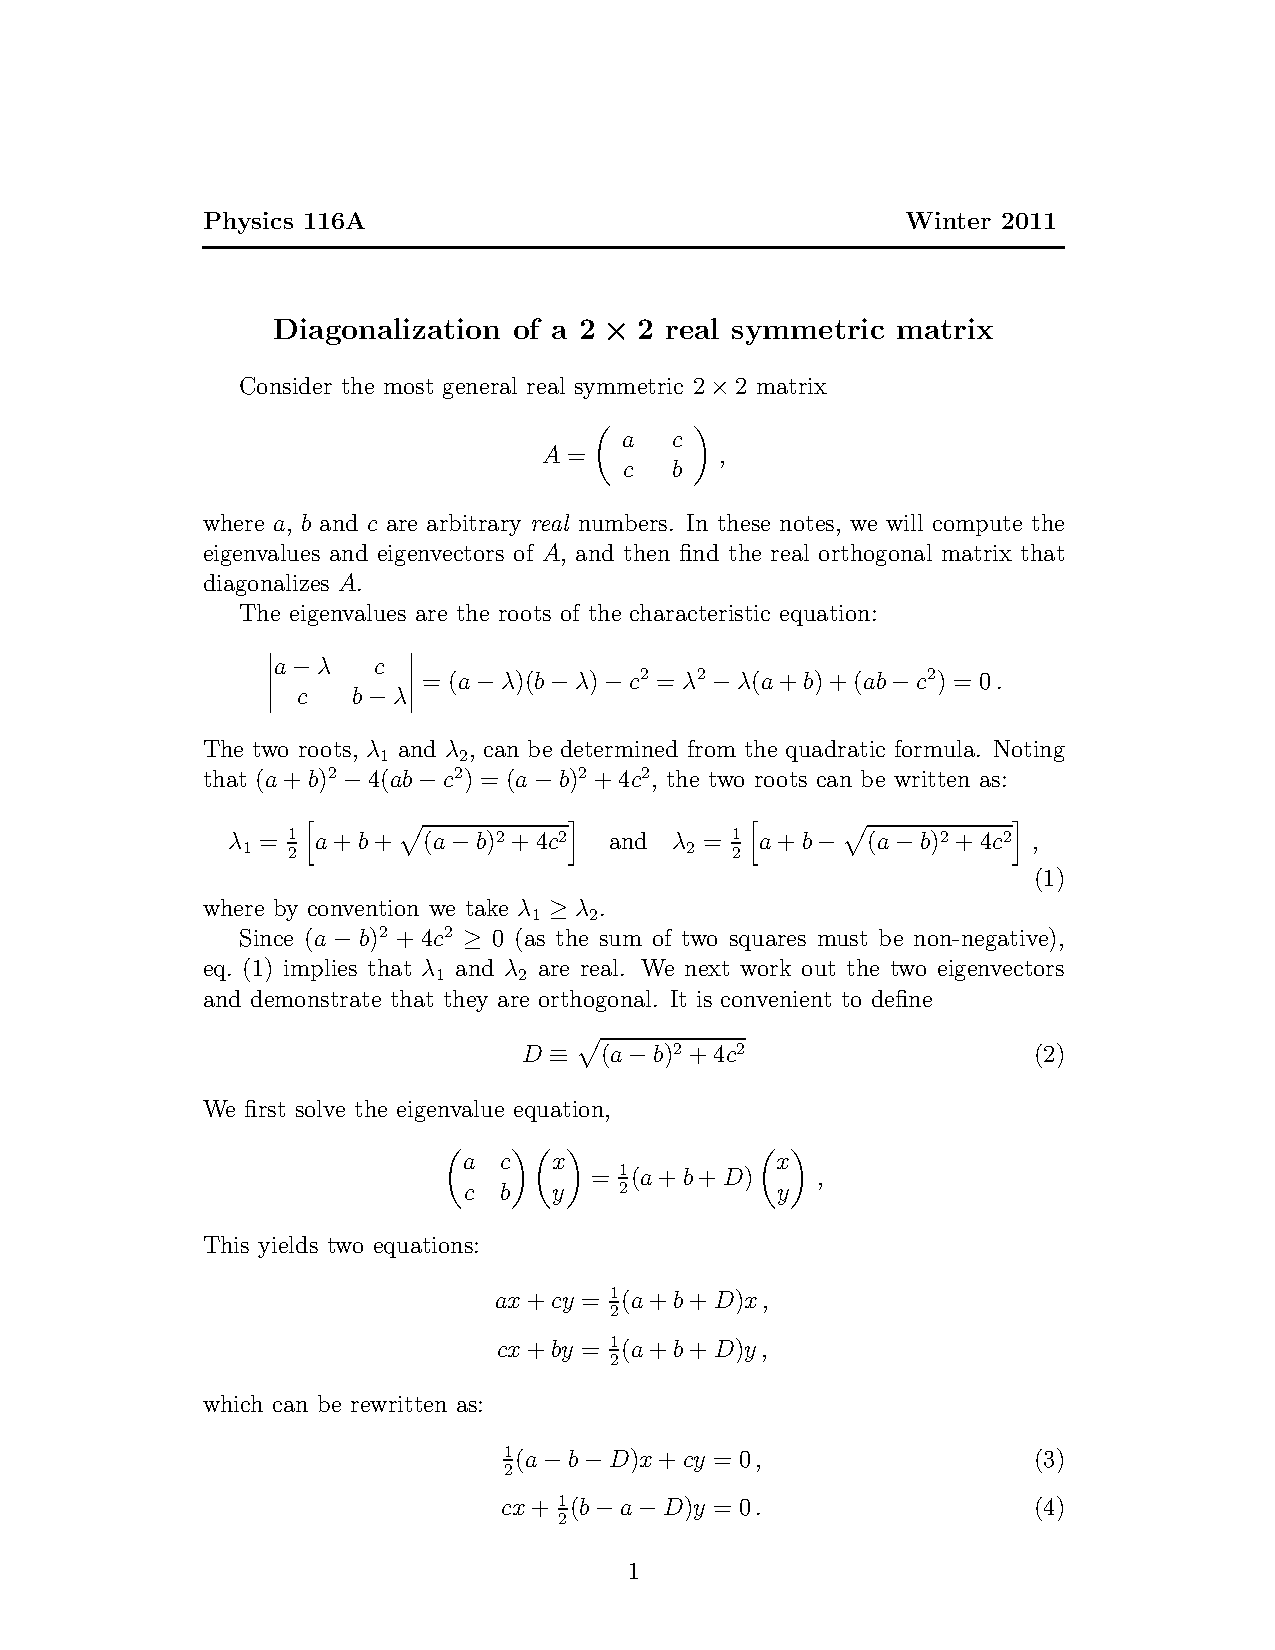
\includepdf[pages=-]{diag2x2.pdf}

From the eigenvalue equations (1) we can easily check that in addition to trace invariance, we have that 
\begin{align}
  \lambda_1-\lambda_2=\sqrt{\left( a-b \right)^2-4c^2}\,.
\end{align}
Replacing back in eq. (9)
\begin{align}
  \sin2\theta=\frac{2c}{\lambda_1-\lambda_2}\,.
\end{align}


%%% Local Variables: 
%%% mode: latex
%%% TeX-master: "beyond"
%%% End:
\begin{thebibliography}{99}
\bibitem{lsm} Diego Restrepo, Hac\'\i a la teor\'\i a cu\'antica de campos, curso web, \url{http://gfif.udea.edu.co}

\bibitem{Maggiore:2005qv}
  M.~Maggiore,
  ``A Modern introduction to quantum field theory,''
%\href{http://www.slac.stanford.edu/spires/find/hep/www?irn=6374123}{SPIRES entry}
{\it  Oxford University Press, 2005. (Oxford Series in Physics, 12. ISBN 0 19 852073 5)}

\bibitem{Mandl:1985bg}
  F.~Mandl and G.~Shaw,
  %``Quantum Field Theory,''
%\href{http://www.slac.stanford.edu/spires/find/hep/www?irn=1457594}{SPIRES entry}
{\it  Chichester, Uk: Wiley ( 1984) 354 P. ( A Wiley-interscience Publication)}

\bibitem{Lahiri:2005sm}
  A.~Lahiri and P.~B.~Pal,
  ``A first book of quantum field theory,''
%\href{http://www.slac.stanford.edu/spires/find/hep/www?irn=6927483}{SPIRES entry}
{\it  Harrow, UK: Alpha Sci. Int. (2005) 380 p}

\bibitem{physics/0703214} Pal, P. ``Representation-independent manipulations with Dirac matrices and spinors'',
	arXiv:physics/0703214v2 [physics.ed-ph]

\bibitem{PD} Wikipedia article: \url{http://en.wikipedia.org/wiki/Particle_decay}

\bibitem{Klasen:2002xi}
  M.~Klasen,
  %``Calculating two- and three-body decays with FeynArts and FormCalc,''
  Int.\ J.\ Mod.\ Phys.\  C {\bf 14} (2003) 1273
  [arXiv:hep-ph/0210426].
  %%CITATION = IMPAE,C14,1273;%%

\bibitem{PeterRenton} \emph{Electroweak Interactions}, Peter Renton


\bibitem{Peskin}
Michael E. Peskin and Daniel V. Schroeder. \emph{An introduction to
Quantum Field Theory}, Addison-Wesley Publishing Company(1995), p.
101

\bibitem{Peskin1}
ibdg 1, p. 105

\bibitem{Halzen}
Francis Halzen and Alan D. Martin. \emph{Quarks} \& \emph{Leptons:
An introductory Course in Modern Particle Physics}, John Wiley \&
Sons(1984), p. 89

\bibitem{Quigg}
Chris Quigg. \emph{Gauge theory of the Strong, Weak and
Electromagnetic Interactions}, Westview Press(1997), p. 110


\bibitem{Quigg1}
ibdg 4, p. 130.

\bibitem{Mandl1}
ibdg 5, p. 325.


\bibitem{Sierra:2008wj}
  D.~Aristizabal Sierra, J.~Kubo, D.~Restrepo, D.~Suematsu and O.~Zapata,
  ``Radiative seesaw: Warm dark matter, collider and lepton flavour violating
  signals,''
  Phys.\ Rev.\  D {\bf 79} (2009) 013011
  [arXiv:0808.3340 [hep-ph]].
  %%CITATION = PHRVA,D79,013011;%%

\bibitem{Gross:1993} 
Relativistic Quantum Mechanics and Field Theory, Franz Gross, John Wiley \& Sons, INC. 1993

\bibitem{McMahon:2009zz}
  D.~McMahon,
  ``Quantum field theory demystified: A self-teaching guide,''
  \href{http://www.slac.stanford.edu/spires/find/hep/www?irn=8432112}{SPIRES entry}
{\it  New York, USA: McGraw-Hill (2009) 299 p}

\bibitem{Feynman:1986er}
  R.~P.~Feynman,
  ``QED. The Strange Theory Of Light And Matter,''
%\href{http://www.slac.stanford.edu/spires/find/hep/www?irn=1631209}{SPIRES entry}
{\it  Princeton, Usa: Univ. Pr. ( 1985) 158 P. ( Alix G. Mautner Memorial Lectures)}


\bibitem{Semenov:2008jy}
  A.~Semenov,
  ``LanHEP - a package for the automatic generation of Feynman rules in field
  theory. Version 3.0,''
  Comput.\ Phys.\ Commun.\  {\bf 180} (2009) 431
  [arXiv:0805.0555 [hep-ph]], \url{http://feynrules.phys.ucl.ac.be/}.
  %%CITATION = CPHCB,180,431;%%

\bibitem{Christensen:2008py}
  N.~D.~Christensen and C.~Duhr,
  ``FeynRules - Feynman rules made easy,''
  Comput.\ Phys.\ Commun.\  {\bf 180}, 1614 (2009)
  [arXiv:0806.4194 [hep-ph]],
   \url{http://feynrules.phys.ucl.ac.be/}.
  %%CITATION = CPHCB,180,1614;%%

\bibitem{massivephoton}
  Christianto V., Smarandache F., and Lichtenberg F., 
  ``\href{http://www.ptep-online.com/index_files/2009/PP-16-08.PDF}{A Note of Extended Proca Equations and Superconductivity,}''
  Progress in Physics, \textbf{1} (2009) 40
  [viXra:1003.0054]

\bibitem{Martin}Martin, Many body quantum field theory

\bibitem{Dreiner:2008tw}
  H.~K.~Dreiner, H.~E.~Haber and S.~P.~Martin,
  ``Two-component spinor techniques and Feynman rules for quantum field theory and supersymmetry,''
  Phys.\ Rept.\  {\bf 494} (2010) 1
  doi:10.1016/j.physrep.2010.05.002
  [arXiv:0812.1594 [hep-ph]].
  %%CITATION = doi:10.1016/j.physrep.2010.05.002;%%
  %185 citations counted in INSPIRE as of 18 May 2016

\bibitem{Roncadelli:1983ty}
  M.~Roncadelli and D.~Wyler,
  ``Naturally Light Dirac Neutrinos in Gauge Theories,''
  Phys.\ Lett.\  {\bf 133B} (1983) 325.
  doi:10.1016/0370-2693(83)90156-9
  %%CITATION = doi:10.1016/0370-2693(83)90156-9;%%
  %84 citations counted in INSPIRE as of 30 Mar 2018
  
\bibitem{Suematsu:2017kcu}
  D.~Suematsu,
  ``Dark matter stability and one-loop neutrino mass generation based on Peccei–Quinn symmetry,''
  Eur.\ Phys.\ J.\ C {\bf 78} (2018) no.1,  33
  doi:10.1140/epjc/s10052-018-5519-4
  [arXiv:1709.02886 [hep-ph]].
  %%CITATION = doi:10.1140/epjc/s10052-018-5519-4;%%
  %5 citations counted in INSPIRE as of 21 Aug 2019

  
\end{thebibliography}
%%% Local Variables: 
%%% mode: latex
%%% TeX-master: "beyond"
%%% End:

\end{document}


%%% Local Variables: 
%%% mode: latex
%%% TeX-master: "beyond"
%%% End: